\documentclass[11pt]{article}
\usepackage{tikz,setspace}
\usetikzlibrary{calc}
\usetikzlibrary{fit}
\usepackage[round]{natbib}
\usepackage[margin=1in]{geometry}
\onehalfspacing
\usepackage{amsmath,setspace,amssymb,amsthm,subfig,url,multicol,microtype}

\frenchspacing

\DeclareMathOperator{\E}{E}
\DeclareMathOperator{\var}{var}
\DeclareMathOperator{\cov}{cov}
\DeclareMathOperator*{\plim}{plim}
\DeclareMathOperator*{\rank}{rank}
\DeclareMathOperator{\tr}{tr}
\DeclareMathOperator{\atan}{atan*}
\newcommand{\newacronym}[3]{%
\expandafter\newcommand\expandafter{\csname #1\endcsname}{#2 \textsc{(\MakeLowercase{#3})}%
\expandafter\renewcommand\expandafter{\csname #1\endcsname}{\textsc{\MakeLowercase{#3}}}}}

\newcommand{\sh}{\hat{\sigma}}
\newcommand{\oosA}{\bar{D}_{R}}
\newcommand{\oosB}{\bar{D}_{T}}

\newcommand{\oost}{\ensuremath{\operatorname{oos-\mathit{t}}}}
\newcommand{\oosSum}[2]{\ensuremath{\sum_{#1=R+#2}^{T-\h}}}

\newcommand{\h}{h}
\newcommand{\InnerBlockL}[1]{\ensuremath{R+(#1-1)b_T + 1}}
\newcommand{\InnerBlockU}[1]{\ensuremath{R+#1 b_T}}
\newcommand{\OuterBlockU}{\lfloor P/b_T \rfloor}
\newcommand{\SumOuterBlock}[1]{\ensuremath{\sum_{#1=1}^{\OuterBlockU}}}
\newcommand{\SumInnerBlock}[2]{\ensuremath{\sum_{#1=\InnerBlockL{#2}}^{\InnerBlockU{#2}}}}

\newcommand{\CEOuterBlock}[2]{\ensuremath{\E_{\InnerBlockU{(#2-1)}} #1}}

\newcommand{\ZSummand}{D_s - \E_R D_s}
\newcommand{\ZDef}{P^{-1/2} \SumInnerBlock{s}{i} [\ZSummand]}
\newcommand{\ZSqCE}{\ensuremath{\CEOuterBlock{Z_i^2}{i}}}
\newcommand{\ZTrunc}{\ensuremath{C\sqrt{b_{T}/P}}}
\newcommand{\PScaleTerm}{\ensuremath{\frac{C \sqrt{b_T}}{P}}}

\newcommand{\vWeight}{W((t-s)/\gamma)}
\newcommand{\vSummand}{\ensuremath{(D_t - \E_R D_t)(D_s - \E_R D_s) \vWeight}}
\newcommand{\kernelBDefn}[1]{\ensuremath{\delta^{-1}(2\pi)^{-1/2}}e^{-#1^2/2\delta^2}}
\newcommand{\kernelB}[1]{\ensuremath{\eta_{\delta}(#1)}}

\newcommand{\vtSum}{\ensuremath{\sum_{t=-P+1}^{2P}}}
\newcommand{\vtSumr}{\ensuremath{\sum_{i=1}^r}}
\newcommand{\vtSuma}{\ensuremath{\sum_{t=(2i-2)b_T-P+1}^{(2i-1)b_T-P}}}
\newcommand{\vtSumb}{\ensuremath{\sum_{t=(2i-1)b_T-P+1}^{2ib_T-P}}}
\newcommand{\vttLower}{\ensuremath{\max(1-t,-b_T)}}
\newcommand{\vttUpper}{\ensuremath{\min(P-t,b_T)}}

\newcommand{\varianceTermIDefn}{\ensuremath{P^{-1}\oosSum{s,t}{1}
    \vSummand}}
\newcommand{\varianceTermI}{\ensuremath{\sigma_{0,\delta}^2}}
\newcommand{\varianceTermII}{\ensuremath{\sigma_{1,\delta}^2}}
\newcommand{\varianceTermIIa}{\ensuremath{(P\gamma)^{-1/2}
    \sum_{l=\max(1-t,-P)}^{\min(P-t,P)} (D_{t+l+R} - \E_R D_{t+l+R})
    W(l/\gamma)}}
\newcommand{\varianceTermIIb}{\ensuremath{(P\gamma)^{-1/2}
    \sum_{j=1-t}^{P-t} (D_{t+j+R} - \E_R D_{t+j+R})
    \kernelB{j/\gamma}}}
\newcommand{\varianceTermIII}{\ensuremath{\sigma_{2,\delta}^{2}}}
\newcommand{\varianceTermIIIa}{\ensuremath{(P\gamma)^{-1/2}
    \sum_{l=\vttLower}^{\vttUpper} (D_{t+l+R} - \E_R D_{t+l+R})
    W(l/\gamma)}}
\newcommand{\varianceTermIV}{\ensuremath{\sigma_{3,\delta}^{2}}}
\newcommand{\varianceTermIVb}{\ensuremath{(P\gamma)^{-1/2}
    \sum_{j=\vttLower}^{\vttUpper} (D_{t+j+R} - \E_R D_{t+j+R})
    \kernelB{j/\gamma}}}
\newcommand{\vtIIIsummand}{\ensuremath{(Z_{1t}Z_{2t} - \E_RZ_{1t}Z_{2t})}}

\newcommand{\varianceDiffA}{\ensuremath{P^{-1} \oosSum{s,t}{1}
    \lvert (D_s - \E_R D_s)(\E_R D_t - \oosA) \rvert
    \vWeight}}
\newcommand{\varianceDiffAi}{\ensuremath{P^{-1} \oosSum{s}{1}(\E_R
    D_s - \oosA )^2}}
\newcommand{\varianceDiffAii}{\ensuremath{P^{-1} \oosSum{s}{1}
    (D_s - \E_R D_s)^2}}

\newcommand{\rhoExp}{\ensuremath{(\rho-2)/2\rho}}
\newcommand{\absReg}{\ensuremath{\rho/(\rho-2)}}

\newcommand{\couplingConstant}{\ensuremath{2^{(1+\rho)/\rho} B_L}}
\newcommand{\couplingBeta}[1]{\ensuremath{\beta^{(\rho-2)/2\rho}_{#1}}}
\newcommand{\couplingBetaSq}[1]{\ensuremath{\beta^{(\rho-2)/\rho}_{#1}}}
\newcommand{\couplingBound}[1]{\couplingConstant \couplingBeta{#1}}

\newcommand{\OCoef}{\ensuremath{O_p(\frac{\sqrt{P}}{T})}}

\newcommand{\bh}[1]{\ensuremath{\hat\theta_{#1}}}
\newcommand{\ep}[1]{\ensuremath{\boldsymbol{\varepsilon}_{#1}}}

\newcommand{\olsMatrix}[2]{\ensuremath{(#1'#1)^{-1}#1'#2}}

\newcommand{\aic}{\textsc{aic}}
\newcommand{\bic}{\textsc{bic}}
\newcommand{\dmw}{\textsc{dmw}}
\newcommand{\ols}{\textsc{ols}}
\newcommand{\mds}{\textsc{mds}}
\newcommand{\clt}{\textsc{clt}}
\newcommand{\lln}{\textsc{lln}}
\newacronym{VAR}{Vector Autoregression}{VAR}
\newacronym{oos}{out-of-sample}{OOS}
\newcommand{\dgp}{\textsc{dgp}}
\newcommand{\hac}{\textsc{hac}}
\newacronym{ned}{Near Epoch Dependent}{NED}
\newacronym{mse}{Mean Squared Error}{MSE}
\newcommand{\sfield}{$\sigma$-field}
\newcommand{\sfields}{\sfield s}
\renewcommand{\Re}{\ensuremath{\mathbb{R}}}

%%% Local Variables: 
%%% mode: latex
%%% TeX-master: paper.tex
%%% End: 

\usepackage[charter]{mathdesign}
\usepackage[osf]{sourcecodepro}
% This will make copy and pasting easier, and will prevent the
% abomination that is monospace font ligatures.  Sorry, everyone who
% really likes ligatures.  Don't worry, the Bitstream Charter font
% has very, very few ligatures anyway.
\DisableLigatures{family = tt*}
\urlstyle{same}

\newcommand{\e}{\varepsilon}
\newcommand{\eb}{\mathbf{\e}}
\DeclareMathOperator{\eigen}{\lambda}

\pagestyle{myheadings}
\newtheorem{thm}{Theorem}
\newtheorem{lem}{Lemma}
\newtheorem{claim}{Claim}
\newtheorem{cor}{Corollary}
\newtheorem{asmp}{Assumption}
\newtheorem{example}{Example}
\newtheorem{defn}{Definition}

\newcommand{\citepos}[1]{\citeauthor{#1}'s \citeyearpar{#1}}
\newcommand{\Citepos}[1]{\Citeauthor{#1}'s \citeyearpar{#1}}
\newcommand{\clws}{\citeauthor{ClW:06}'s \citeyearpar{ClW:06,ClW:07}}

\usepackage[bitstream]{mathdesign}

% VERSION is generated by a post-commit hook and contains the git
% version info
\IfFileExists{VERSION}{
  \input{VERSION}
  \date{\dinfo\ (commit \hinfo)}
  \markright{\dinfo\ (commit \hinfo)}
}{}

\title{Out-of-Sample Comparisons of Overfit Models}
\author{Gray Calhoun\thanks{email: gcalhoun@iastate.edu. I
    would like to thank Julian Betts, Helle Bunzel, Marjorie Flavin,
    Nir Jaimovich, Lutz Kilian, Ivana Komunjer, Michael McCracken,
    Seth Pruitt, Ross Starr, Jim Stock, Yixiao Sun, Allan Timmermann,
    Hal White, several anonymous referees, participants at the 2010
    Midwest Economics Association Annual Meetings, the 2010
    International Symposium on Forecasting, the 2010 Joint Statistical
    Meetings, the 2011 NBER-NSF Time-Series
    Conference, and in many seminars at UCSD, and espeically
    Graham Elliott for their valuable suggestions, feedback and advice
    in writing this paper.  I would also like to thank Amit Goyal for
    providing computer code and data for his 2008 RFS paper
    with Ivo Welch \citep{GoW:08}.} \\ Iowa State University}

\begin{document}
\maketitle

\begin{abstract}\thispagestyle{empty}\noindent
  This paper uses dimension asymptotics to study why overfit linear
  regression models should be compared out-of-sample; we let the
  number of predictors used by the larger model increase with the
  number of observations so that their ratio remains uniformly
  positive.  Our analysis gives a theoretical motivation for using
  out-of-sample (OOS) comparisons: the DMW OOS test allows a forecaster to
  conduct inference about the expected future accuracy of his or her
  models when one or both is overfit.  We show analytically and
  through Monte Carlo that standard full-sample test statistics can
  not test hypotheses about this performance.  Our paper also shows
  that popular test and training sample sizes may give misleading
  results if researchers are concerned about overfit.  We show that
  $P^2/T$ must converge to zero for the DMW test to give valid
  inference about the expected forecast accuracy, otherwise the test
  measures the accuracy of the estimates constructed using only the
  training sample.  In empirical research, $P$ is typically much
  larger than this.  Our simulations indicate that using large values
  of $P$ with the DMW test gives undersized tests with low power, so
  this practice may favor simple benchmark models too much.

\noindent JEL Classification: C12, C22, C52, C53

\noindent Keywords: Generalization Error, Forecasting, Model
Selection, $t$-test, Dimension Asymptotics
\end{abstract}
\newpage

\section{Introduction}\label{sec:introduction}
Consider two sequences of length $P$ of prediction errors, the result
of forecasting the same variable with two different estimated models.
Both models are estimated with $R$ observations, collectively called
the {\em estimation window}, and are used to forecast an additional
$P$ observations, called the {\em test sample}.  There are $T$
observations in all, and $R+P=T$.  This paper introduces a new limit
theory for statistics constructed from these prediction errors
designed to approximate the behavior of the statistics when one of the
models is overfit.  In doing so, we provide a theoretical
justification for forecasters to use OOS instead of in-sample
comparisons: the DMW OOS test%
\footnote{In this paper, we will refer to the basic OOS $t$-test
  studied by \citet{DiM:95} and \citet{Wes:96} as the DMW test.} %
allows a forecaster to conduct
inference about the expected future accuracy of his or her models when
one or both is overfit.  We show analytically and through Monte Carlo
that standard full-sample test statistics can not test hypotheses
about this performance.

Our paper also shows that popular test and training sample sizes may
give misleading results if researchers are concerned about overfit.
We show that $P^2/T$ must converge to zero for the DMW test to give
valid inference about the expected forecast accuracy, otherwise the
test measures the accuracy of the estimates constructed using only the
training sample.  In empirical research, $P$ is typically much larger
than this.  Our simulations indicate that using large values of $P$
with the DMW test gives undersized tests with low power, so this
practice may favor simple benchmark models too much.  Existing
corrections, proposed by \citet{ClM:01,ClM:05}, \citet{Mcc:07} and
\citet{ClW:06,ClW:07}, seem to overcorrect for this problem, though, and reject
too often when the benchmark model is more accurate.


Although OOS comparisons have been popular in Macroeconomics and
Finance since \citepos{MeR:83} seminal study of exchange rate models,
it has been unclear from a theoretical perspective whether or not the
statistics are useful.  Empirical researchers often cite ``overfit''
or ``instability'' as reasons for using OOS comparisons, as in
\citet{StW:03}, but neither term is precisely defined or formalized.
Compounding this problem, the asymptotic distributions of these
statistics are derived under conditions that rule out either
instability or overfit and allow a researcher to use a conventional
in-sample comparison---a variation of the $F$-test, for example.  As
\citet{InK:04} argue, the statistics themselves are designed to test
hypotheses that can be tested by these in-sample statistics.  For
example, \citet{DiM:95} and \citet{Wes:96} derive the limiting
distributions of many popular OOS test statistics under conditions
that would justify these full-sample tests.  Much
of the subsequent research by \citet{Mcc:00, Mcc:07}, \citet{CCS:01},
\citet{ClM:01,ClM:05}, \citet{CoS:02,CoS:04}, \citet{ClW:06,ClW:07},
\citet{Ana:07}, and others relaxes several of Diebold and Mariano's
and West's assumptions, but maintains the stationarity and dependence
conditions that permit in-sample comparisons \citep[see][for a
review of this literature]{Wes:06}.%
\footnote{Like us, \citet{Ana:07} allows the number of regressors to
  increase with $T$.  But in that paper, the number of regressors
  increases slowly enough that the OLS coefficients are consistent and
  asymptotically normal.} %
\citet{GiW:06} and
\citet{GiR:09, GiR:10} are exceptions.  Instead of focusing on
hypotheses that can be tested by in-sample comparisons, \citet{GiW:06}
derive an OOS test for the null hypothesis that the difference
between two models' OOS forecasting performance is unpredictable, a
martingale difference sequence; \citet{GiR:09} test whether the OOS
forecasting performance of a model suffers from a breakdown relative
to its in-sample performance; and \citet{GiR:10} test whether the
forecasting performance is stable. However, those papers focus on a
particular OOS estimation strategy and do not address why OOS
comparisons might be useful as a general strategy.

Since in-sample and OOS statistics require similar assumptions and
test similar hypotheses, one might expect that they would give similar
results.  They do not.  In-sample analyses tend to support more
complicated theoretical models and OOS analyses support simple
benchmarks, as seen in \citet{MeR:83}, \citet{StW:03}, and
\citet{GoW:08}.  Since these different approaches strongly influence
the outcome of research, it is important to know when each is
appropriate.  The explanations in favor of OOS comparisons claim
that they should be more robust to unmodeled instability
\citep{ClM:05,GiW:06,GiR:09,GiR:10} or to overfit
\citep{Mcc:98,Cla:04}.  Both explanations presume that the in-sample
comparison is invalid and the OOS comparisons are more reliable.  Of
course, as \citet{InK:04,InK:06} point out, both in-sample and OOS
methods could be valid, but the OOS methods could have lower power.

In this paper, we study the ``overfit'' possibility and leave
``instability'' to future research. This paper uses dimension
asymptotics to study the behavior of OOS comparisons when at least
one of the models is overfit---the number of its regressors
increases with the number of observations so that their ratio remains
positive.  Although overfit is sometimes used to describe the
situation where a forecaster chooses from many different models,
i.e. \textit{data-mining} or \textit{data-snooping}, we view these as
separate issues.  Procedures that account for the presence of many
models have been, and are continuing to be, developed \citep[see, for
example,][]{Whi:00,Han:05,RoW:05,HHK:10,ClM:12b}, but it is unclear
whether those procedures should themselves use in-sample or OOS
comparisons.  Understanding the difference between in-sample and OOS
comparisons in the context of a simple comparison between two models
is necessary before resolving any new issues that arise with multiple
comparisons. Moreover, the empirical research that motivates
this paper uses \textit{pseudo} OOS comparisons and not
\textit{true} OOS comparisons.  Even if a true OOS comparison
could account for some forms of data-snooping better than
\citepos{Whi:00} BRC or its extensions, in-sample and pseudo
OOS comparisons would both be affected by the data-snooping, a
point also made by \citet{InK:04}.

We focus on linear regression models estimated with a fixed window
for simplicity, but our basic
conclusions should be true for other models as well.  Under this
asymptotic theory, where the number of regressors $k$ increases with $T$
so that $\lim k/T$ is positive and less than one,
the OLS coefficient estimator is no longer
consistent or asymptotically normal \citep{Hub:73} and has positive
variance in the limit.  We show that, even so, the usual OOS average
is asymptotically normal and can consistently estimate the difference
between the models' generalization error, the expected loss in the
future conditional on the on the data available in period
$T$.%
\footnote{See, for example, \citet{HTF:08} for a discussion of
  generalization error.} %
Under these asymptotics, the generalization
error does not converge to the expected performance of the pseudo-true
models, so existing in-sample and OOS comparisons measure different
quantities and should be expected to give different results for
reasons beyond simple size and power comparisons.  Under our limit theory,
the model that is closer to the true DGP in population can forecast
worse.  In such a situation, a standard in-sample comparison would
correctly reject the null hypothesis that the benchmark is true, and
an OOS comparison would correctly fail to reject the null that the
benchmark is more accurate.%
\footnote{In a pair of papers similar to
  ours, \citet{ClM:12,ClM:12b} study in-sample and OOS tests that
  the larger model has nonzero coefficients that are too close to zero
  to expect the model to forecast more accurately.  Like this paper,
  they argue that the larger model can be true but less accurate.
  However, they focus on an aspect of the DGP that makes this
  phenomenon likely, while we focus on the coefficient estimates that
  produce less accurate forecasts.  Moreover, the implications of our
  asymptotic theories are different and their papers do not provide
  reasons to do OOS comparisons.} %
Also note that, in this situation, a model that performs well
in-sample can perform badly out-of-sample even if there are no
structural breaks or other forms of instability.  Researchers
have argued that a breakdown of in-sample forecasting ability
indicates a structural break (see \citealp{BoH:99} and
\citealp{StW:03} among others), but this breakdown can be caused by overfit as
well.

Our results can justify OOS comparisons when researchers want to
choose a model for forecasting.  Although there has been little
emphasis on hypothesis testing in this setting, testing is usually
appropriate: there is usually a familiar benchmark model in place, and
the cost of incorrectly abandoning the benchmark for a less accurate
alternative model is higher than the cost of incorrectly failing to
switch to a more accurate alternative.  We show that the DMW test
lets the forecaster control the probability of the first error, just
as with conventional hypothesis testing.

But we also identify new practical limitations for applying the DMW
test to overfit models.
Since the models' coefficients are imprecisely estimated in the limit,
the test sample must be small enough that the model estimated over the
training sample is similar to the one that will be estimated over the
full sample.  In particular, $P/T \to 0$ is required for consistent
estimation of the difference in the two models' performance,
and $P^2/T \to 0$ is required for valid confidence
intervals and inference.  For larger $P$, the OOS comparisons remain
asymptotically normal, but are centered on the forecasting performance
associated with the period-$R$ estimates.  In practice, researchers
typically use large values of $P$, so these studies may be too
pessimistic about their models' future accuracy if they use the DMW
test.  Section~\ref{sec:oostheory} lays out the asymptotic behavior of
the DMW test under this limit theory.

Popular in-sample tests and model selection criteria, like the Wald
test, AIC, and BIC, do not help forecasters in this setting. We show
that these statistics can no pick out the more accurate model. For
many DGPs they will choose a larger alternative model over a small
benchmark model with probability approaching one, regardless of which
model is more accurate.%
\footnote{Our result holds for a broad class of
  full-sample statistics, but there may be other potential statistics
  that mimic the OOS test and remain valid. Exploring such
  statistics is left for future research.} %
This result holds even though modifications of the $F$-test are valid
under this asymptotic theory, as shown by \citet{BoB:95},
\citet{AkA:00}, \citet{AkP:04}, \citet{Cal:11c}, and \citet{Ana:12},
among others.%
\footnote{Also see \citet{Efr:86,Efr:04} for a discussion
  of naive in-sample loss comparisons.} %
Moreover, under this asymptotic theory, many recent OOS test
statistics, such as those derived by \cite{ClM:01,ClM:05},
\citet{Mcc:07}, and \citet{ClW:06,ClW:07} should have the same
problems as in-sample tests.%
\footnote{Our theoretical results apply
  directly to \citepos{Mcc:07} OOS $t$-test, since it simply
  proposes more liberal critical values for the same test statistic
  that we study.  Since \citet{ClW:06,ClW:07} use a finite length
  estimation window, our asymptotics are incompatible with theirs and
  prevent us from studying their test directly, as well as
  \citepos{GiW:06} and other tests based on \citepos{GiW:06}
  asymptotics.  But \clws\ test can be viewed as a stochastic
  adjustment to the critical values of the usual OOS $t$ test, so
  our conclusions should apply informally as well.  Specifically, we
  show that the DMW test rejects with probability equal to nominal
  size when the estimated benchmark model is expected to be more
  accurate, so more liberal critical values result in overrejection.} %
These tests are also designed to reject the benchmark when the
alternative model is true, and so they may reject too often when the
benchmark is false but more accurate.  Obviously, since the
distribution of these statistics converges to the normal when $P/T \to
0$ (with the number of regressors fixed), these statistics behave like
the DMW test when $P$ is small, but should overreject the benchmark
when $P$ is large. Section~\ref{sec:insample} presents our theoretical
results for full-sample statistics and Section~\ref{sec:mc} presents
Monte Carlo evidence to support these claims.

Finally, this paper also introduces a new method of proof for OOS
statistics.  We use a coupling argument (Berbee's Lemma, 1979) to show
that sequences of OOS loss behave like mixingales when the
underlying series are absolutely regular, even if the forecasts depend
on non-convergent estimators.  Moreover, transformations of these
processes also behave like mixingales when recentered, so 
the arguments used to prove asymptotic
results for Near Epoch Dependent (NED) functions of mixing processes
can be used for these OOS processes with only slight modification.

The rest of the paper proceeds as follows.
Section~\ref{sec:assumptions} introduces our notation and assumptions.
Section~\ref{sec:theory} gives the main theoretical results for the
DMW OOS test, shows that standard in-sample tests reject the
benchmark model too often when it is false but more accurate than the
alternative, and shows that standard model selection methods choose the
larger model too often under similar conditions. Section~\ref{sec:mc}
presents a Monte Carlo study supporting our theoretical results.
Section~\ref{sec:empirics} applies the OOS statistic to
\citepos{GoW:08} dataset for equity premium prediction, and
Section~\ref{sec:conclusion} concludes.  Proofs and supporting results
are listed in the Appendix.

\section{Setup and assumptions}\label{sec:assumptions}

The first part of this section will describe the environment in detail
and set up our models and notation. The second part will list the
assumptions underlying our theoretical results.

\subsection{Notation and forecasting environment}
We assume the following forecasting environment. There are two
competing linear models that give forecasts for the target,
$y_{t+\h}$:
\begin{equation}
y_{t+\h} = x_{1t}'\theta_1 + \e_{1,t+h}, \quad\text{and}\quad
y_{t+\h} = x_{2t}'\theta_2 + \e_{2,t+h};
\end{equation}
$t = 1,\dots,T-h$, $\h$ is the forecast horizon and the
variables $y_t$, $x_{1t}$, and $x_{2t}$ are all known in period $t$.
The coefficients $\theta_1$ and $\theta_2$ minimize the population
Mean Square Error, so
\begin{equation}
  \theta_i = \argmin_\theta \sum_{t=1}^{T-\h} \E (y_{t+\h} - x_{it}'\theta)^2,
\end{equation}
making $\e_{i,t+\h}$ uncorrelated with $x_{i,t}$; $\e_{i,t+\h}$ can exhibit
serial correlation so both of the linear models may be misspecified.
Let $\mathcal{F}_t = \sigma(y_1, x_1, \dots, y_t, x_t)$ be the information
set available in period $t$,
with $x_t$ the vector of all stochastic elements of $x_{1t}$ and $x_{2t}$ after
removing duplicates, and let $\E_t$ and $\var_t$ denote the
conditional mean and variance given $\mathcal{F}_t$.  The first model
uses $K_1$ regressors, and the second uses $K_2$.  Without loss of
generality, assume that $K_1 \leq K_2$. At least one of the models is
overfit, which we represent asymptotically by letting $K_2$ grow with
$T$ quickly enough that $\lim K_2/T$ is positive; $K_1$ may grow with
$T$ as well. Since the models change with $T$, a
stochastic array underlies all of our asymptotic theory, but we
suppress that notation to simplify the presentation.

In the settings we are interested in, a forecaster observes the data
$(y_t,x_t)$ for periods 1 through $T$ and divides the observations
into an estimation sample of the first $R$ observations and a test
sample of the remaining $P$ observations. The forecaster then compares
the models' performance over the test sample, which entails
constructing two sequences of forecasts, (using a fixed-window
estimation strategy)
\begin{equation}
\hat y_{i,t+\h} = x_{it}'\hat{\theta}_{it}, \qquad \text{for } i=1,2;
\ t = R+1,\dots,T-h,
\end{equation}
where
\begin{equation}
  \bh{it} = \Big(\sum_{s=1}^{R-\h} x_{is}x_{is}'\Big)^{-1} \sum_{s=1}^{R-\h}
  x_{is} y_{s+\h}, \qquad \text{for } i=1,2;\ t = R+1,\dots, T - \h.%
\footnote{It may not be clear why we are using a $t$ index in $\bh{it}$,
    since $\bh{it} = \bh{iR}$ almost surely for all $t \leq T-h$.
    But $\bh{it}$ will be defined for $t > T-\h$
    soon and will not equal $\bh{iR}$ for those values of $t$.} %
\end{equation}

The models are then compared by their forecast errors over the test
sample.  There are many statistics that have been considered in the
literature, but we focus on perhaps the most natural, the DMW \oost\
test \citep{DiM:95,Wes:96}.%
\footnote{The core insights of our paper apply to other OOS statistics
  as well.} %
This statistic is based on
the difference in the models' loss over the test sample, $\oosA$,
defined as
\begin{equation}
  \oosA \equiv P^{-1} \oosSum{t}{1} D_t
\end{equation}
where
\begin{equation}\label{eq:16}
  D_t = L(y_{t+\h} - x_{1t}'\bh{1t}) - L(y_{t+\h} - x_{2t}'\bh{2t}),
\end{equation}
and $L$ is a known loss function. The \oost\ test is defined as
$\sqrt{P} \oosA / \sh$, where $\sh^2$ is an estimator of the
asymptotic variance of $\oosA$. (Possibly a Heteroskedasticity- and
Autocorrelation-Consistent, or HAC, estimator.)

Most theoretical research, such as \citet{DiM:95}, \citet{Wes:96},
and \cite{Mcc:07}, has focused on using the \oost\ statistic to test
hypotheses about the pseudo-true values $\theta_1$ and $\theta_2$.  In
particular, that research focuses on testing the null hypothesis that
\begin{equation}\label{eq:21}
  \E L(y_{t+\h} - x_{1t}'\theta_{1}) - \E L(y_{t+\h} - x_{2t}'\theta_{2}) = 0.
\end{equation}
But the population quantities in \eqref{eq:21} do not determine which
model is more accurate in finite samples and, under our asymptotics,
in the limit when models are allowed to be overfit. The models'
accuracy will also depend on the specific estimates of $\theta_1$ and
$\theta_2$ used to produce the forecasts. In this setting, where the
forecaster will use one of the models to make a number of predictions
in the future---call the number of predictions $Q$---the quantity of
interest becomes
\begin{equation}
  \E_T \oosB \equiv Q^{-1} \sum_{t=T+1}^{T+Q} \E_T D_t,
\end{equation}
where $D_t$ is defined in Equation~\eqref{eq:16} but here uses the
full-sample estimates of the models' parameters,
\begin{equation}
  \bh{it} = \Big(\sum_{s=1}^{T-\h} x_{is}x_{is}'\Big)^{-1} \sum_{s=1}^{T-\h}
  x_{is} y_{s+\h}, \qquad \text{for } i=1,2;\ t = T+1,\dots, T + Q.
\end{equation}
If $\E_T \oosB$ is positive, the second model is expected to forecast
better than the first over the next $Q$ periods, and if $\E_T \oosB$
is negative then the first model is better. We use a conditional
expectation because the coefficient estimates in $\oosB$ are
stochastic but known in period $T$, and their values will determine
the performance of the two models.

Under conventional fixed-$K$ asymptotic theory, $\E_T \oosB$ would
converge in probability to the difference in the expected loss
associated with the pseudo-true models,%
\footnote{Under standard stationarity, moment, and weak-dependence
  conditions.} %
i.e. the LHS of~\eqref{eq:21}.
\begin{equation}\label{eq:22}
  \E L(y_{t+\h} - x_{1t}'\theta_{1}) - \E L(y_{t+\h} - x_{2t}'\theta_{2}).
\end{equation}
But if $K_2$ increases with $T$ these quantities can have different
limits. For a simple example, assume squared-error loss, let $x_{1,t}
= 1$ for all $t$, and let $(y_{t+\h},x_{2,t})$ be i.i.d. $N(0,
\Sigma)$.  Then
\begin{align*}
  \E_T \oosB - & \big(\E L(y_{t+\h} - x_{1t}'\theta_{1}) - \E L(y_{t+\h} - x_{2t}'\theta_{2})\big) \\
  &= \big(\E_T (y_{T+\h+1} - \bh{1,T})^2 - \E_T (y_{T+\h+1} - x_{T+1}'\bh{2,T})^2\big) -
  \big(\E y_{T+\h+1}^2 - \E (y_{T+\h+1} - x_{T+1}'\theta_2)^2 \big)\\
  &= (\bh{2,t} - \theta_2)' \Sigma_x (\bh{2,t} - \theta_2) + o_p(1).
\end{align*}
This last term has expectation $\var(y_T) \frac{K_2}{T - K_2 - 1}$ and
would converge to zero if $K_2$ were fixed, but does not when $\lim
K_2 / T > 0$. In Section~\ref{sec:oostheory} we show that the \oost\
statistic can estimate $\E_T \oosB$ under our increasing $K$
asymptotics and does not estimate the expected loss associated with
the pseudo-true coefficients.

The conditional expectation $\E_T \oosB$ has been studied heavily in
cross-sectional settings with independent observations. In such a
setting, $\E_T \oosB$ is equal to the difference in the models'
\emph{generalization error}, which has been used widely as a measure
of model accuracy in the machine
learning literature \citep[see][for further discussion]{HTF:08}.
Moreover, with i.i.d. observations, the expectation of $\E_T \oosB$
equals \citepos{Aka:69} Final Prediction Error (FPE). Both
generalization error and FPE are defined by a model's
performance on a new, independent, data set, but, for lack of a better
term, we will call $\E_T \oosB$ the difference in generalization error
for the rest of the paper with hopefully no risk of confusion.

Finally, define the following notation.  The $l_v$-norm for vectors in
$\Re^p$ (with $p$ arbitrary) is denoted $\lvert \cdot \rvert_v$, and
the $L_v$-norm for $L_v$-integrable random variables is $\lVert \cdot
\rVert_v$.  The functions $\eigen_i(\cdot)$ take a square-matrix
argument and return its $i$th eigenvalue (with $\eigen_{i}(A) \leq
\eigen_{i+1}(A)$ for any matrix $A$).  All limits are taken as $T \to
\infty$ unless stated otherwise.

\subsection{Assumptions}

The next conditions are assumed to hold throughout the paper.  The first
assumption controls the dependence of the underlying random array.
The second lays out the details of our asymptotic approximation.
The third assumption controls the
smoothness of the loss function and bounds the moments of the
difference in the models' performance; the fourth assumption describes
the behavior of the estimation and test windows.  And the last
assumption describes the kernel used to estimate the OOS average's
asymptotic variance.

\begin{asmp}\label{asmp-1}
  The random array $\{y_t,x_t\}$ is stationary and absolutely regular
  with coefficients $\beta_j$ of size $-\rho/(\rho-2)$; $\rho$ is
  greater than two and discussed further in Assumption \ref{asmp-3}.
\end{asmp}

This assumption is a standard condition on the dependence of the
underlying stochastic array. The only novelty is that we use
absolute regularity instead of strong or uniform mixing as our
weak dependence condition; absolute regularity admits a particular
coupling argument, ``Berbee's Lemma'' \citep[reproduced in this
paper as Lemma A.1 for reference]{Ber:79} that is
unavailable for strong mixing sequences; absolute regularity
implies uniform mixing, so this assumption is not unduly strong.
For a detailed discussion of these weak dependence conditions,
please see, for example, \citet{Dav:94}.

Our strict stationarity assumption is also somewhat stronger than is
typically used; \citet{Wes:96} and \citet{Mcc:07}, for example,
present results assuming covariance stationarity of the loss
associated with the pseudo-true models. We need to make a stronger
assumption because we will need to prove asymptotic results where the
$\bh{it}$ remain random---so we would need covariance stationarity to
hold for almost all estimates of $\theta_i$, and not just for the
pseudo-true value.

The next assumption describes our asymptotic experiment.
\begin{asmp}\label{asmp-2}
  The number of regressors for each model, $K_1$ and $K_2$, are less
  than $R$, and $K_2/T$ and $(K_2-K_0)/T$ are uniformly positive;
  $K_0$ is the number of regressors shared by the two models ($K_1/T$
  can be uniformly positive as well, but is not required to be).

  The variance of $y_{t+\h}$ given $\mathcal{F}_t$ is uniformly
  positive and finite, and all of the eigenvalues of the covariance
  matrix of $x_t$ are uniformly positive and finite as well.
  Moreover,
  \begin{align*}
    &\eigen_{\max}(X_{iS}'X_{iS}) = O_{L_3}(S),&
    &\eigen_{\max}(\E(X_{iT}'\ep{iT}\ep{iT}'X_{iT}
    \mid X_{iR}'X_{iR}, X_{iT}'X_{iT})) = O_{L_3}(S),\\
    &\eigen_{\max}((X_{iS}'X_{iS})^{-1}) = O_{L_3}(1/S),&
    &\eigen_{\max}\Big(\E\Big( \sum_{s,t=R+1}^{T-h} \e_{is} \e_{it} x_{is}x_{it}'
    \,\Big|\, X_{iR}'X_{iR} \Big)\Big) = O_{L_3}(P),
  \end{align*}
  for large enough $T$, where $S = R,T$, $i = 1,2$,
  \[ X_{iT} \equiv [x_{i1} \quad \dots \quad x_{i,T-\h}]' \qquad
  \text{and} \qquad \ep{iT} = (\e_{i,1+\h}, \dots, \e_{i,T})'.\]

  Additionally, the Euclidean norms of the pseudo-true coefficients,
  $\theta_1$ and $\theta_2$, satisfy $|\theta_1|_2 = O(1)$ and
  $|\theta_2|_2 = O(1)$.
\end{asmp}

The assumption that $y_{t+\h}$ and $x_t$ have positive and finite
variance is straightforward.  The conditions on the eigenvalues are
technical and control the behavior of the OLS estimator as the
number of regressors gets large.  The restrictions on the pseudo-true
coefficients ensure that the regression model doesn't dominate the
variance of $y_{t+\h}$ in the limit.

We can see that these conditions are trivially satisfied when the
underlying series are i.i.d.\ Normal and the regression includes a
constant.
\begin{example}
  If $(x_{t}, y_t)$ are i.i.d. $N(0, \Sigma)$ where $\Sigma$ is
  uniformly positive definite, then
  \begin{equation*}
    \theta = \cov(y_t, x_t) \var(x_t)^{-1}
  \end{equation*}
  and the regression constant is
  \begin{equation*}
    \theta_0 = \E y_t - \cov(y_t, x_t) \var(x_t)^{-1} \E x_t
  \end{equation*}
  where both of these terms follow directly from the normality
  assumption.  Then $|\theta|_2 = O(1)$ as a consequence of uniform
  positive definiteness of $\Sigma$ and $\varepsilon_t \sim i.i.d.\
  N(0, v^2)$ (independent of $x_t$) with
  \begin{equation*}
    v^2 = \var(y_t) - \cov(y_t, x_t) \var(x_t)^{-1} \cov(y_t, x_t)'.
  \end{equation*}
  Then we have
  \begin{equation*}
    \E(X_{T}'\ep{T}\ep{T}'X_T \mid X_{R}'X_{R}, X_{T}'X_{T})
    = v^2 X_{T}'X_{T}
  \end{equation*}
  and
  \begin{equation*}
    \E\Big( \sum_{s,t=R+1}^{T-h} \e_s \e_t x_s x_t'
    \,\Big|\, X_{R}'X_{R} \Big) = P v^2 \E x_t x_t'.
  \end{equation*}

  So the conditions amount to restrictions on the eigenvalues of
  $X_T'X_T$, which are familiar from general OLS.
\end{example}

The next assumption establishes moment conditions for the OOS loss
process and smoothness conditions for the loss function itself. The
moment conditions are standard and apply to $D_t$, and the smoothness
conditions are relatively weak.

\begin{asmp}\label{asmp-3}
  The loss function $L$ is continuous, has finite left and right
  derivatives, and $L(0) = 0$.  There is a constant $B_L$ and a
  function $L'$ that bounds the left and right derivative of $L$ at
  every point such that $\|D_t\|_\rho \leq B_L$; $\|D_t^*\|_\rho \leq
  B_L$ for all $t$, where
  \begin{equation*}
    D_t^* = L(y^* - x_1^{*\prime}\hat\theta_{1t})
    - L(y^* - x_2^{*\prime}\hat\theta_{2t})
  \end{equation*}
  and $(y^*, x_1^*, x_2^*)$ equals $(y_t, x_{1t}, x_{2t})$ in
  distribution but is independent of $\mathcal{F}_T$ ($\rho$ is defined
  in Assumption~\ref{asmp-1}); and
  \begin{equation*}
    \| L'(y^* - x_{i}^{*\prime}
    (\alpha \hat{\theta}_{iR} + (1-\alpha) \hat{\theta}_{iT})) \|_2
    \leq B_L
  \end{equation*}
  for any $\alpha \in [0,1]$.
\end{asmp}

The differentiability condition in Assumption~\ref{asmp-3} is weak and
allows the loss function itself to be non-differentiable; for example,
absolute error and many asymmetric loss functions satisfy this
assumption.  The next assumption controls the growth of the test and
training samples.
\begin{asmp} \label{asmp-4} $P, R, Q \to\infty$ and $P^2/T \to 0$ as
  $T \to \infty$.
\end{asmp}

The requirements that $P$ and $R$ grow with $T$ are common. Parts of
the assumption are new, in particular the requirement that $P^2/T \to
0$.  See Lemma~\ref{res-convergence} for a discussion of its
implications.  In practical terms, this assumption requires that the
test sample be large and that the training sample be much larger, by
enough that including or excluding the test sample does not affect the
estimates of $\theta_1$ or $\theta_2$ very much.

A final assumption restricts the class of variance estimators we will
consider.  We use the same class of estimators studied by
\citet{JoD:00} (their class $\mathcal{K}$); see
their paper for further discussion.

\begin{asmp}
  \label{asmp-5} $W$ is a kernel from
$\Re$ to $[-1,1]$ such that $W(0) = 1$, $W(x) = W(-x)$ for all $x$,
\begin{equation*}
  \int_{-\infty}^{\infty} \lvert W(x) \rvert dx < \infty, \quad
  \int_{-\infty}^{\infty} \lvert \psi(x) \rvert dx < \infty
\end{equation*}
with
\begin{equation*}
  \psi(x) = \frac1{\sqrt{2\pi}} \int_{-\infty}^{\infty} W(z) e^{ixz}dz,
\end{equation*}
and $W(\cdot)$ is continuous at zero and all but a finite number of
points.
\end{asmp}

Assumptions~\ref{asmp-1}--\ref{asmp-5} are broadly similar to
\citepos{Wes:96} assumptions, except with regard to model complexity
and the size of the test sample.  West assumes that $K_1$ and $K_2$
are both finite, while we let them grow rapidly with $T$
(Assumption~\ref{asmp-1}), and West lets $P/R$ converge to any value
in $[0,\infty]$, while we require $P^2/R \to 0$
(Assumption~\ref{asmp-4}).%
\footnote{\citet{Wes:96} does not have a
  second OOS period, so there is no analogue in his paper to our
  restriction on $Q$.} %
Obviously, these differences are
related---allowing for complex models requires tighter constraints on
the size of the test sample.  West allows more general estimation
methods, while we restrict attention to OLS; the advantage of using
OLS is that we can derive the inequality,
\begin{equation*}
  \| x_{it}'\bh{i,T+1} - x_{it}'\bh{iR} \|_2 \leq O(P/T)^{1/2}.
\end{equation*}
Our main results will hold for other models and estimation windows as
long as a similar inequality exists, but proving such inequalities is
left for future research.

Our other assumptions are similar.  The loss function must be smooth
almost everywhere, which is less restrictive than \citet{Wes:96}
requires but is not new; \citet{Mcc:00} extends West's results to
cover a similar case.\footnote{Our assumptions allow for discontinuous
  loss functions, such as those proposed by \citet{PeT:92}.
  \citet{Mcc:00} does not explicitly allow for such loss functions,
  but it appears that his conclusions hold for them as well under the
  restriction $P/T \to 0$.}  We assume full stationarity and absolute
regularity of the underlying random array, while West assumes
covariance stationarity and strong mixing of the transformed forecast
errors; and the details our moment conditions are different, but seem
that they would hold in similar environment to West's.  Finally, since
West's is a more standard environment, he assumes the existence of a
consistent estimator of the variance, while we construct it
explicitly.  Only West's assumptions governing model complexity and
the size of the test sample are substantially different than ours.

\section{Theoretical Results}\label{sec:theory}
The main result of the paper is Theorem
\ref{res-confidence-intervals}, which shows that the OOS average is
asymptotically normal and centered on $\E_T \oosB$.  This result holds
even for nested models and can be used to construct confidence
intervals or test hypotheses.  After presenting Theorem
\ref{res-confidence-intervals}, we explain and present two key Lemmas
used in its proof that add some insight into the nature of OOS
comparisons, and then show that standard HAC OOS estimators can be
used to consistently estimate the asymptotic variance of the OOS
average.  We next present an example that illustrates some of these
concepts, and then show that typical full-sample tests do not let
researchers test hypotheses about $\E_{T} \oosB$ when the models are
overfit.  In fact, in the limit they can reject a more accurate but
false benchmark model almost surely.

\subsection{Behavior of the DMW Test with Overfit}\label{sec:oostheory}
Our first theorem justifies using the DMW $t$-test with a a short
test sample.

\begin{thm}\label{res-confidence-intervals}
  Suppose that Assumptions \ref{asmp-1}--\ref{asmp-4} hold, that
  $\sh^2$ is an estimator satisfying
  \[
    \sh^2 - \sigma^2 \to^p 0 \quad \text{with}\quad
    \sigma^2 \equiv \var_R(\sqrt{P} \oosA) \equiv P \E_R(\bar{D}_R -
    \E_R \bar{D}_R)^2,
  \]
  and that $\sigma^2$ is uniformly a.s. positive.  Then
  \[
  \frac{\oosA - \E_T\oosB}{\sh / \sqrt{P}}
  \to^d N(0,1).
  \]
  Consequently, each of the usual Gaussian confidence intervals,
  \begin{gather}
  [\oosA - z_{\alpha/2} \, \sh /
      \sqrt{P}, \oosA + z_{\alpha/2} \sh / \sqrt{P}],\label{interval-twosided} \\
  [\oosA - z_{\alpha} \, \sh / \sqrt{P}, +\infty), \label{interval-greater}
  \intertext{and}
(-\infty, \oosA + z_{\alpha}
      \, \sh / \sqrt{P}],
    \end{gather}
    contains $\E_T\oosB$ with probability $\alpha$ in the limit,
  with $z_{\alpha}$ the $1-\alpha$ quantile of the standard normal
  distribution.
\end{thm}
The requirement that $\sigma^2$ be uniformly a.s. positive is not
restrictive under our asymptotic theory.  Since the models'
coefficients are estimated with uncertainty in the limit, the two
models give different forecasts even if they both nest the DGP.  This
is intuitively similar to \citepos{GiW:06} rolling-window result, but
comes from different asymptotic theory; Giacomini and White keep the
variance of the OOS average positive by letting $P \to \infty$ with
$R$ fixed; in this paper, $R \to \infty$ but the variance remains
positive since $K \to \infty$ (quickly) as well.

This result allows forecasters to use the DMW test to conduct
inference about the models' accuracy.  Since the OOS average,
$\oosA$, is asymptotically normal and centered on the expected future
performance, $t$-tests constructed from the OOS errors necessarily
test hypotheses about $\E_T \oosB$ and not the performance of the
pseudo-true models or the unconditional performance of the
models.\footnote{i.e. $\E L(\e_{1,t+\h}) - \E  L(\e_{2,t+\h})$ or $\E \oosB$.
Note that the expectation of $\E_T \oosB$ equals $\E \oosB$ but that
$\sqrt{P} (\E_T \oosB - \E \oosB)$ may not be asymptotically normal,
which would be necessary for testing.}
This application to testing can be expressed as its own theorem:
\begin{thm}\label{res:oostest}
Suppose that the conditions of Theorem \ref{res-confidence-intervals}
hold and that $\lim \Pr[\E_T \oosB \leq 0] > 0$.  Then
\begin{equation}
  \lim \Pr[P^{1/2}\oosA/\sh > z_{\alpha} \mid \E_T
  \oosB \leq 0] \leq \alpha.
\end{equation}
\end{thm}

Two intermediate Lemmas will help us understand Theorem
\ref{res-confidence-intervals} better.  Its proof consists of two
steps: we can write
\begin{equation}
  \sqrt{P} (\oosA - \E_T \oosB) = \sqrt{P} (\oosA - \E_R
  \oosA) + \sqrt{P} (\E_R \oosA - \E_T \oosB),
\end{equation}
so Theorem~\ref{res-confidence-intervals} holds if
\begin{equation}\label{coefpart}
  \E_R \oosA = \E_T \oosB + o_p(P^{-1/2}).
\end{equation}
and
\begin{equation}\label{normalpart}
  \sqrt{P}\frac{\oosA - \E_R \oosA}{\sigma} \to^d N(0,1)
\end{equation}
The first Lemma establishes~\eqref{coefpart} and the second shows that
the process $\{D_t - \E_R \oosA\}$ is an $L_2$-mixingale of size
$-1/2$ that satisfies a CLT, ensuring~\eqref{normalpart}.

\begin{lem} \label{res-convergence}
  Under Assumptions \ref{asmp-1}--\ref{asmp-4},
  \begin{equation}\label{eq:7}
    \E_T \oosB - \E_R \oosA = O_p(\sqrt{P/T}) + o_p(P^{-1/2} + Q^{-1/2}).
  \end{equation}
\end{lem}

Note that $\E_T \oosB - \E_R \oosA$ is noise introduced by
approximating the performance of the full-sample estimates with that
of the partial-sample estimates.  Moreover, the $O_p(\sqrt{P/T})$ term
is binding; it is straightforward to find examples for which
$\sqrt{T/P}(\E_T \oosB - \E_R \oosA)$ does not converge to
zero.\footnote{Notice that, if the observations are i.i.d. and
  $(y_{t+h}, x_{it}) \sim N(0,I)$, $(\hat{\theta}_{iR} -
  \hat{\theta}_{iT}) \sim N(0, (X_{iR}'X_{iR})^{-1} -
  (X_{iT}'X_{iT})^{-1})$ given $X_{iT}$, and so
  $\var(x_{i,T+1}'\hat{\theta}_{iR} - x_{i,T+1}'
  \hat{\theta}_{iT}) \gg P K_i / (R - K_2)(T - K_2)$.}
Consequently, there is little scope to relax our assumption that
$P^2/T \to 0$.  If $\lim P^2/T$ is positive and finite then there is
the possibility of adjusting the asymptotic distribution of the test
statistic to account for this noise term as in \citet{Wes:96}, but we
leave that to future research.  If $P^2/T \to \infty$, which is
closest to common practice in applied research, the noise term
dominates the asymptotic distribution of the OOS $t$-test and the
test has only trivial power in the limit if it has correct size.

\begin{lem}\label{res-mixingale}
  Part 1: If Assumptions~\ref{asmp-1}--\ref{asmp-3} hold then the
  inequality
  \begin{equation}\label{mixingaleR}
    \lVert \E_{R+j-l}(D_{R+j} - \E_R D_{R+j}) \rVert_2 \leq
    \couplingConstant \; \zeta_l
  \end{equation}
  with $\zeta_l = O(l^{-1/2 - \delta})$ holds for some positive
  $\delta$, any positive $j$, and any $l$ between 0 and $j$.  As a
  consequence, $\{D_t - \E_R D_t, \mathcal F_t\}$ is an
  $L_2$-mixingale of size $-1/2$.

  \noindent Part 2: Moreover,~\eqref{normalpart} holds under
  Assumptions~\ref{asmp-1}--\ref{asmp-4} if $\sigma^2$ is
  a.s. uniformly positive.
\end{lem}

Mixingales satisfy a weak-dependence condition similar to MDSes and
were introduced and studied extensively by
\citet{Mcl:74,Mcl:75,Mcl:75b,Mcl:77}.  This lemma shows that the
estimation uncertainty introduces dependence into the OOS forecast
errors, but the additional dependence is contained in the term $\E_R
\oosA$ and can be effectively removed by subtraction.  The second part
of the Lemma shows that the basic mixingale CLT established by
\citet{Jon:97} applies in this setting.\footnote{De Jong proves two
  CLTs: one for mixingales and one for NED functions of mixing
  processes.  His mixingale result makes assumptions about the
  behavior of the sample second moment that arise as consequences of
  NED.  The proof of Lemma~\ref{res-mixingale} shows that the
  arguments used for de Jong's NED CLT continue to hold for our
  OOS process---in effect, that the OOS process has slightly more
  structure than required for it to be a mixingale.}  Note that
Lemma~\ref{res-mixingale} does not require $P^2/T \to 0$.

Finally, for Theorem \ref{res-confidence-intervals} to be useful, we
need a consistent estimator of $\sigma^2$. Lemma
\ref{res-variance-estimator} establishes that the usual OOS HAC
variance estimators are consistent.\footnote{As with
      Lemma~\ref{res-mixingale}, the proof of this lemma takes
      \citepos{JoD:00} existing consistency results
      for NED processes and shows that the same arguments can be
      applied to our OOS mixingale.}

\begin{lem}
  \label{res-variance-estimator} Suppose Assumptions
  \ref{asmp-1}--\ref{asmp-5} hold and that $\gamma \to \infty$ and
  $\gamma/P \to 0$ as $T \to \infty$, and define
  \begin{equation*}
    \sh^2 \equiv P^{-1} \oosSum{s,t}{1} (D_t - \oosA)(D_{Rs} - \oosA)
    \vWeight.
  \end{equation*}
  Then $\sh^2 - \sigma^2 \to^p 0$.
\end{lem}

The next subsection presents an example that clarifies the previous
results.

\subsection{An Example}\label{sec:example}

Let $L(e) = e^2$, let $h
= 1$, let the benchmark model have no regressors (i.e. $y_{t+1} \sim$
white noise), suppose that $(y_{t}, x_{2t}) \sim i.i.d.\ N(0,I)$, and
assume that $R > 2K_2 + 4$.\footnote{The restriction $R > 2 K_2 + 4$
  allows us to use a convenient formula for moments of the
  Inverse-Wishart distribution.}  Under these conditions,
\begin{equation*}
  D_t =
  \begin{cases}
    2 y_{t+1} x_{2t}'\hat{\theta}_{2R} -
    \hat{\theta}_{2R}' x_{2t} x_{2t}' \hat{\theta}_{2R} & t \leq T \\
    2 y_{t+1} x_{2t}'\hat{\theta}_{2T} -
    \hat{\theta}_{2T}' x_{2t} x_{2t}' \hat{\theta}_{2T} & t > T.
  \end{cases}
\end{equation*}

The first two conditional moments of $D_t$ for $t > R$ (given
$\mathcal{F}_R$) are straightforward to derive: $\E_R D_t = -
\hat{\theta}_{2R}' \hat{\theta}_{2R}$ and
\begin{equation*}
  \sigma^2 \equiv \E_R(D_t - \E_R D_t)^2 = 4
  \hat{\theta}_{2R}' \hat{\theta}_{2R} +
  \E_R(\hat{\theta}_{2R}' (I - x_{2t} x_{2t}')
  \hat{\theta}_{2R})^2   \geq 4 \hat{\theta}_{2R}'
  \hat{\theta}_{2R} \quad a.s.
\end{equation*}
Now, $\hat{\theta}_{2R}' \hat{\theta}_{2R}$ is
a.s. positive and uniformly integrable with mean $4 K_2 / (R - K_2 -
1)$ (since $(X_{2R}'X_{2R})^{-1}$ is Inverse-Wishart$(I_{K_2}, R)$),
making $\sigma^2$ uniformly a.s. positive and ensuring that the
distribution of the OOS average is not $P^{1/2}$-degenerate.  The
natural OOS variance estimator is consistent for $\sigma^2$:
\begin{align*}
  \sh^2 &= P^{-1} \sum_{t=R+1}^{T-1} (D_t - \oosA)^2 \\
  &= 4 \hat{\theta}_{2R}' \Big[P^{-1} \sum_{t=R+1}^{T-1}
  \Big(y_{t+1} x_{2t} - P^{-1} \sum_{s=R+1}^{T-1} y_s x_{2s}\Big)
  \Big(y_{t+1} x_{2t} - P^{-1} \sum_{s=R+1}^{T-1} y_s
  x_{2s}\Big)'\Big] \hat{\theta}_{2R}' \\ & \quad - 4
  \Big[P^{-1} \sum_{t=R+1}^{T-1} \Big(y_{t+1} x_{2t} - P^{-1}
  \sum_{s=R+1}^{T-1} y_s x_{2s}\Big)' \hat{\theta}_{2R}
  \hat{\theta}_{2R}' \Big(x_{2t} x_{2t}' - P^{-1}
  \sum_{s=R+1}^{T-1} x_{2s} x_{2s}' \Big) \hat{\theta}_{2R} \Big]
  \\ &\quad + P^{-1} \sum_{t=R+1}^{T-1}
  \Big[\hat{\theta}_{2R}' \Big(x_{2t} x_{2t}' - P^{-1}
  \sum_{s=R+1}^{T-1} x_{2s} x_{2s}' \Big) \hat{\theta}_{2R}  \Big]^{2}.
\end{align*}
As $P \to \infty$, the first term converges in probability to
$\hat{\theta}_{2R}' \hat{\theta}_{2R}$, the second to zero,
and the third to $\E_R(\hat{\theta}_{2R}'(I - x_{2t}x_{2t}')
\hat{\theta}_{2R})^2$.  Since the number of regressors prevents
$\hat{\theta}_{2R}$ from converging i.p. to zero (its expected
value), $\sh^2$ does not converge to the unconditional
variance.

We can see that the OOS average obeys a CLT when centered at $\E_R
\bar{D}_R$.  The centered and scaled OOS differences satisfy
\begin{equation*}
  \frac{D_t - \E_R D_t}{\sigma} =
  \frac{2 y_{t} x_{2t}' \hat{\theta}_{2R} +
    \hat{\theta}_{2R}' (I - x_t x_t') \hat{\theta}_{2R}}{\sqrt{4
    \hat{\theta}_{2R}' \hat{\theta}_{2R} +
    \E_R(\hat{\theta}_{2R}'(I - x_{2t} x_{2t}') \hat{\theta}_{2R})^2}}.
\end{equation*}
This sequence is not i.i.d. and we can not replace $\hat{\theta}_{2R}$
with a sequence of constants $\theta_{2R}$ since $\hat{\theta}_{2R}$
does not converge to a deterministic limit.  But $\sigma^{-1}
\E_t(\oosA - \E_R\oosA) = 0$, making this sequence an
MDS,\footnote{The sequence is actually exchangeable, but MDS is
  enough to establish the CLT.} so it obeys a CLT as long as
$\sigma^2$ is uniformly a.s. positive, which we have already
established.  Lemma~\ref{res-mixingale} ensures that the CLT holds
more generally.

Finally, we can look at the difference $\E_R \bar{D}_R - \E_T
\bar{D}_T$.  We can write this as
\begin{align*}
  \E_R \oosA - \E_T \oosB &= \hat{\theta}_{2R}'
  \hat{\theta}_{2R} - \hat{\theta}_{2T}' \hat{\theta}_{2T} \\ &=
  \eb_T'[\tilde{X}_{2R}(X_{2R}'X_{2R})^{-2}
  \tilde{X}_{2R} - X_{2T}(X_{2T}'X_{2T})^{-2} X_{2T} ] \eb_T
\end{align*}
with $\tilde{X}_{2R}$ the $T \times K_2$ matrix $[X_{2R}'\ 0]'$.
Standard results for the moments of quadratic forms and of the
Inverse-Wishart distribution \citep{Haf:79} imply that
\begin{equation*}
  \E(\E_R \oosA - \E_T \oosB) = \frac{K_2 P}{(T - K_2 - 1)(R - K_2 - 1)}
\end{equation*}
and
\begin{align*}
  \var(\E_R & \oosA - \E_T \oosB) \\ &= \E
  \big[\tr((X_{2R}'X_{2R})^{-1} - (X_{2T}'X_{2T})^{-1})\big]^2 + 2 \tr
  \E\big((X_{2R}'X_{2R})^{-2} - (X_{2T}'X_{2T})^{-2}\big) \\ &\quad - \big[\tr
  \E((X_{2R}'X_{2R})^{-1} - (X_{2T}'X_{2T})^{-1}) \big]^2 \\ &=
  O(P/T)^2.
\end{align*}
So, in this example, $P^{1/2}(\E_R \oosA - \E_T \oosB) \to^p 0$
if $P^3/T^2 \to 0$, which is slightly weaker than the general
requirement that $P^2/T \to 0$.  If $\lim P^3/T^2 > 0$ the OOS average
still obeys the MDS CLT, but it is not centered correctly at $\E_T
\oosB$.

\subsection{Failure of in-sample forecast evaluation}\label{sec:insample}
This subsection establishes that in-sample tests like the $F$-test can
overreject when the benchmark is more accurate than the alternative.
The issue explored here is different than that of \citet{Cal:11c} and
\citet{Ana:12}; in those papers, the authors demonstrate that full
sample Wald and $F$-tests can be invalid under increasing-$k$
asymptotics,%
\footnote{\citet{Ana:12} shows that the Wald test is
  invalid in general and gives an adjustment that corrects the
  critical values; he also shows that the $F$-test is asymptotically
  valid under certain conditions on the distribution of the
  regressors.  \citet{Cal:11c} shows that the $F$-test is
  asymptotically invalid without Anatolyev's constraint, and provides
  a correction that gives valid tests.  Both papers only consider
  independent observations.} %
e.g. they can overreject when testing the
null hypotheses that a set of the coefficients is zero.  This paper,
though, looks at the behavior when the coefficients are non-zero but
the estimated restricted model is more accurate.  In this setting,
these tests reject the benchmark too often---more than their nominal
size---and for most coefficient values will reject almost surely in
the limit.  We also look at some common model selection statistics and
find the same conclusion---they choose the larger model with high
probability regardless of which model will forecast better.  To
simplify the presentation, we'll only present results for nested
models.

Theorem~\ref{res:ftest} presents results for in-sample hypothesis
tests.
\begin{thm}\label{res:ftest}
  Suppose Assumptions 1--3 hold, that the models are nested, and that
  $L(e) = e^2$.  Also, let $\Lambda$ be a test statistic with nominal
  size $\alpha$ that has acceptance region contained in the set
  \[\{\hat{\theta}_T \mid (\hat{\theta}_T -
  \theta_0)'V_T(\hat{\theta}_T - \theta_0) < c \}\] for large enough
  $T$ and some $\theta_0$, $c$, and $V_T$, with $V_T$ a possibly
  random matrix with all eigenvalues uniformly bounded in probability
  and rank satisfying $\lim \rank(V_T)/T > 0$.  Then there exist
  distributions for $(x_t, \e_{t+h})$ such that
  \begin{equation}
    \label{eq:11}
    \Pr[\Lambda \text{ rejects} \mid \E_T \oosB \leq 0] \to^p 1
    \quad \text{as} \quad
    \theta'V_T\theta \to^p \infty \quad \text{($T$ is fixed)}
  \end{equation}
  for almost every sequence $\theta$ (a.e. with respect to Lebesgue
  measure) and
  \begin{equation}
    \label{eq:15}
    \plim_{T \to \infty} \Pr[\Lambda \text{ rejects} \mid
    \E_T \oosB \leq 0] \geq \plim_{T \to \infty} \Pr[c + \delta < (\theta - \theta_0)' V_{T}
    (\theta - \theta_0) \mid \E_T \bar{D}_T \leq 0]
  \end{equation}
  for any $\delta > 0$.
\end{thm}
Note that, if $V_T$ is nonstochastic or converges in probability,
there are distributions on $(x_t, \e_{t+h})$ that are
compatible with~\eqref{eq:15} such that
\[\Pr[c + \delta < (\theta - \theta_0)'V_T (\theta - \theta_0) \mid
E_T \bar{D}_T \leq 0] \to^p 1
\]
for any $\theta \neq \theta_0$.  Otherwise, the rejection probability
will still depend on $\theta$ and $V_T$ and will typically be higher
than the nominal size of the test.

Theorem~\ref{res:ftest} covers a broad class of test statistics and
allows the in-sample test to be valid or invalid in finite samples or
asymptotically.  It implies that a large class of in-sample tests will
reject if $\theta$ is nonzero, whether or not the alternative model is
more accurate.  As an example, consider the $F$-test of the null
hypothesis $A \theta =0$ with deterministic regressors and
i.i.d. Normal errors where $\rank A = J$ and $\lim J/T > 0$.  Simple
algebra reveals that the test rejects if $\hat{\theta}_T' V_T
\hat{\theta}_T \geq 1$ with
\begin{equation*}
  V_T = (T/ J \hat{\xi}^{2}) A' (A (T^{-1}X_T'X_T)^{-1} A')^{-1} A;
\end{equation*}
$\xi^2$ is the variance of the model's innovations and $\hat{\xi}^2$ is
the usual estimator based on the squared residuals.  Note that $\rank
V_T = \rank A$ as long as $X_T'X_T$ is full rank.  Under the null $A
\theta = 0$,
\begin{equation*}
  \hat{\theta}_T' V_T
  \hat{\theta}_T =^d   (\xi^2/ J \hat{\xi}^2) \chi_J^2 =^d 1 + J^{-1/2} Z
  + o_p(T^{-1/2}),
\end{equation*}
where $\chi_J^2$ is an independent $\chi^2$ random variable with $J$
degrees of freedom and $Z \sim N(0,1)$.  Consequently, the $F$-test
accepts whenever $\hat{\theta}_T$ is in a neighborhood of the cylinder
defined by $\hat{\theta}_T' V_T \hat{\theta}_T = 1$ and rejects for
$\hat{\theta}_T$ outside the neighborhood.%
\footnote{If $V_T$ is full
  rank, this equation defines an ellipsoid in $\mathbb{R}^K$;
  otherwise the equation defines an ellipsoid in a subspace of
  $\mathbb{R}^K$.} %
The neighborhood shrinks as $T \to \infty$, so the
$F$-test satisfies the conditions of Theorem~\ref{res:ftest} with
$V_T$ as given above and $c = 1 + \delta$ for any $\delta > 0$.
Notice that $c$ does not depend on the nominal size of the test and
that the exact finite sample distribution of the $F$-test is known in
this example, so the test is valid by conventional measures but the
conclusions of Theorem~\ref{res:ftest} still hold.

The intuition behind Equation~\eqref{eq:11} can be understood by
simplifying further to the case $K_2 = 2$ and $K_1 = 0$, deterministic
orthonormal regressors, and $V_T = I$, so
\begin{equation*}
  E_T \oosB = \theta_{1}^2 + \theta_{2}^2 - (\hat{\theta}_{T,1} -
  \theta_{1})^2 - (\hat\theta_{T,2} - \theta_2)^2.
\end{equation*}
Under these conditions, the test rejects if $\hat{\theta}_{T}$ lies
outside the circle centered at the origin with radius $c^{1/2}$ and
$\E_T \oosB \leq 0$ holds for $\hat\theta_{T}$ on or outside a circle
centered at $\theta$ passing through the origin.
Figure~\ref{fig:rreject} depicts these regions.  Since the OLS
estimator is normal with mean $\theta$, the probability that
$\hat{\theta}_{T}$ falls in the acceptance region given $\E_T \oosB
\leq 0$ vanishes as $\theta'\theta \to \infty$, even though the full
model will give worse forecasts than the restricted model.

\newcommand{\circlefigA}[4]{
  \begin{tikzpicture}
    \fill[lightgray] (-#3,-#3) rectangle (#4,#4);
    % rejection region for F-test
    \filldraw[fill=white,draw=black] (0,0) circle (#1);
    % circle of equal generalization error
    \filldraw[fill=white,draw=black] (1,1) let \p1=(1,1) in circle({veclen(\x1,\y1)});
    \draw (1,1) let \p1=(1,1) in circle({veclen(\x1,\y1)});
    \fill [black] (1,1) circle (2pt) node[right] {$(\theta_1,\theta_2)$};
    \draw (0,0) circle (#1);
    \draw (1,1)--(0,0);
    % axes
    \draw[->] (0,0)--(#2,0) node[right] {$\hat\theta_{T,1}$};
    \draw[->] (0,0)--(0,#2) node[above] {$\hat\theta_{T,2}$};
  \end{tikzpicture}
}
\newcommand{\circlefigB}[4]{
  \begin{tikzpicture}
    \fill[white] (-#3,-#3) rectangle (#4,#4);
    % rejection region for F-test
    \fill[lightgray] (0,0) circle (#1);
    % circle of equal generalization error
    \fill[white] (1,1) let \p1=(1,1) in circle({veclen(\x1,\y1)});
    \draw (0,0) circle (#1);
    \draw (1,1) let \p1=(1,1) in circle({veclen(\x1,\y1)});
    \fill [black] (1,1) circle (2pt) node[right] {$(\theta_1,\theta_2)$};
    \draw (1,1)--(0,0);
    % axes
    \draw[->] (0,0)--(#2,0) node[right] {$\hat\theta_{T,1}$};
    \draw[->] (0,0)--(0,#2) node[above] {$\hat\theta_{T,2}$};
  \end{tikzpicture}
}

\begin{figure}
  \centering
  \begin{tabular}{cc}
  \subfloat[]{\circlefigA{1}{2.5}{1.4}{3.2}\label{fig:circleA}} &
  \subfloat[]{\circlefigB{1}{2.5}{1.4}{3.2}\label{fig:circleB}}  \\
  \subfloat[]{\circlefigA{.3}{2.5}{1.4}{3.2}\label{fig:circleC}}  &
  \subfloat[]{\circlefigB{.3}{2.5}{1.4}{3.2}\label{fig:circleD}}
  \end{tabular}
  \caption{Graphs indicating the rejection region and region of equal
    generalization error for the models discussed in Section
    \ref{sec:insample}.  The smaller model has no estimated parameters
    and the larger has two coefficients.  The shaded regions in
    Figures (a) and (b) show the rejection region and the acceptance
    region respectively of the full-sample test given $\E_T \oosB \leq
    0$ when the true elements of $\theta$ are moderately small.  Figures
    (c) and (d) show the same regions when the true $\theta$ is large.}
\label{fig:rreject}
\end{figure}

Equation~\eqref{eq:15} is more interesting and implies that these
tests will almost surely reject the benchmark whenever we have a true
but overfit and less accurate alternative.  The intuition is similar
to the previous case.  As $K_2$ increases, the volume that
$\hat{\theta}_{T}$ can occupy increases as well.  If $\theta$ is
outside the acceptance region, the probability that $\hat{\theta}_{T}$
is close to the origin and therefore inside the acceptance region of
the test decreases.  In the limit, the probability that
$\hat{\theta}_{T}$ is outside the acceptance region is one.

A similar result for model selection follows as a Corollary to
Theorem~\ref{res:ftest}.  Consistent model selection in this context
is different than in the finite-$K$ case.  Here we want the
probability of selecting a model given that it is more accurate to
converge to one.  Formally, a model selection procedure is useful if
\begin{gather}\label{eq:13}
  \Pr[\text{model $1$ selected} \mid \E_T \oosB \leq 0] \to 1
  \intertext{and} \Pr[\text{model $2$ selected} \mid \E_T \oosB > 0]
  \to 1.\label{eq:14}
\end{gather}
Note that the conditioning event in~\eqref{eq:14} is different than in
the testing results presented earlier, but otherwise they are similar.
Theorem~\ref{res:ftest} implies that~\eqref{eq:13} will typically fail
for overfit models for many common model selection methods, including
adjusted $R^2$, the AIC, and the BIC.  Corollary~\ref{res:ic}
contains the details.

\begin{cor}\label{res:ic}
  Suppose the conditions of Theorem~\ref{res:ftest} hold but that the
  statistic $\Lambda'$ is used for model selection; $\Lambda'$ selects
  the benchmark model for all $\hat{\theta}_T$ contained in a subset
  of the region
  \begin{equation*}
    \{\hat{\theta}_T \mid \hat{\theta}_T'V_T \hat{\theta}_T < c\}
  \end{equation*}
  and selects the alternative for all $\hat{\theta}_T$ outside that
  region.  Then there exist distributions on $x_t,\e_t$ such
  that
  \begin{equation}
    \label{eq:17}
    \plim \Pr[\Lambda' \text{ selects model 1} \mid \E_T \bar{D}_T \leq 0]
    \leq \plim \Pr[\theta_0'V_T \theta_0 < c \mid \E_T \bar{D}_T].
  \end{equation}
\end{cor}
As before, we often have
\begin{equation*}
  \Pr[\theta_0'V_T \theta_0 < c \mid \E_T \bar{D}_T] \to^p 0.
\end{equation*}
Just as we saw with the $F$-test, adjusted $R$-squared, the AIC and
the BIC will only choose the benchmark model if $\hat{\theta}_T$
lies in the neighborhood of the cylinder defined by $\hat{\theta}_T
V_{T} \hat{\theta}_T = c$, regardless of which model is expected to
forecast better.  These statistics differ in how they determine the
size of the neighborhood, with the neighborhood shrinking slower for
the BIC than the AIC.

It is important to remember that the tests considered do not need to
have correct size for the null $\theta = \theta_0$, but are allowed to
in this analysis, so previous research, such as \citet{Cal:11c} and
\citet{Ana:12}, does not predict these results.  However, these tests
are poorly suited for choosing an accurate forecasting model and
perform worse when the larger model is overfit or explains more of the
variation of the dependent variable.  Essentially, for forecasting we
want to know if the coefficient estimates are close to their true
values, but in-sample statistics tell us only whether the estimates
are close to a particular hypothesized value (usually zero).  There
are lots of estimates that are both far from zero and far from their
true values which cause in-sample statistics to incorrectly choose the
alternative model.

\section{Monte Carlo}\label{sec:mc}
\newcommand{\thetanorm}{\ensuremath{\lvert \theta \rvert_2}} This
section presents two simulations that investigate the accuracy of our
theory in small samples.\footnote{Simulations were conducted in R
  \citep{Rde:10} using Sweave \citep{Lei:02} and the Lattice
  \citep{Sar:10}, RSQLite \citep{Jam:10}, tikzDevice
  \citep{ShB:11:0.6.1}, and pgfSweave \citep{BrS:11:1.2.1} packages.}
The first looks at the asymptotic normality of the DMW statistic
centered on either $\E_R \oosA$ or $\E_T \oosB$.  The previous
section's results imply that centering on the first should give an
approximately normal statistic and centering on the second should give
a normal statistic when $P$ is small relative to $T$.  The second
simulation looks at the size and power of several statistics when
conducting inference about the difference in the models'
generalization error.  For all of the simulations, we look at
fixed-window OOS tests to speed up computation time.

\subsection{Setup}\label{sec:simulation-design}
The Monte Carlo experiment is intentionally very simple so that we can
isolate the influence of the models' complexity.  In particular, we do
not include some features that are common in forecasting
environments---serial dependence, heteroskedasticity, and complicated
DGPs.  We simulate data for both studies from the equation
\begin{equation}\label{eq:6}
  y_t = x_t'\theta + \e_t,\quad \e_t \sim N(0,1),
  \quad t=1,\dots,T.
\end{equation}
The first element of $x_t$ is 1 and the remaining $K_2-1$ elements are
independent Standard Normal.  The benchmark model is
\begin{equation}
  \label{eq:1}
  y_{1t} = \sum_{j=1}^{K_1} x_{jt}\theta_j + \e_t
\end{equation}
and the alternative model is the DGP \eqref{eq:6}.  We let
$(K_1,K_2)$ equal either $(2,3)$ or $(T/20,T/10)$ to study our theory
in its intended application as well as for more parsimonious models.
We let $T$ equal 100, 250, 500, or 1000.  We also vary $\theta$, and do
so giving the benchmark and the alternative model comparable weight in
predicting $y_t$.  Specifically, we set
\begin{equation*}
  \theta_j =
\begin{cases} \frac{c}{\sqrt{K_1}} & j = 1,\dots,K_1 \\
\frac{c}{\sqrt{K_2 - K_1}} & j = K_1 + 1,\dots,K_2 \end{cases}
\end{equation*}
with $c$ equal to zero or one.  When $c$ is one, we're more likely to
draw values of $X$ and $Y$ that make the estimated larger model more
accurate than the benchmark, and when $c$ is zero we're unlikely to
draw such values of $X$ and $Y$.  For all of the studies, $L(x) =
x^2$.

The first set of simulations study how well the theory in
Section~\ref{sec:oostheory} works in practice.  For each draw of $X$
and $Y$, we construct a one-sided OOS interval of the
form
\begin{equation*}
  [ \oosA - 1.28 \hat{\sigma}, \infty) \quad\text{with}\quad
  \sh^2 = \frac1P \sum_{t=R+1}^T (D_t - \oosA)^{2}
\end{equation*}
for $P$ set to every 10th value between 1 and $2T/3$.  We calculate
the percentage of these intervals that contain $\E_R \oosA$ and that
contain $\E_T \oosB$.  Since the data are i.i.d., both of these
quantities are easy to calculate:
\begin{equation*}
  E_R \oosA = \Bigg[\sum_{i=1}^{K_1} (\tilde{\theta}_{iR} - \theta_i)^2 +
  \sum_{i=K_1+1}^{K_2}\theta_i^2\Bigg] - \sum_{i=1}^{K_2} (\hat{\theta}_{iR} -
  \theta_i)^2
\end{equation*}
and
\begin{equation*}
  E_T \oosB = \Bigg[\sum_{i=1}^{K_1} (\tilde{\theta}_{iT} - \theta_i)^2 +
  \sum_{i=K_1+1}^{K_2}\theta_i^2\Bigg] - \sum_{i=1}^{K_2} (\hat{\theta}_{iT} -
  \theta_i)^2
\end{equation*}
where $\tilde{\theta}$ indicates that the coefficient is estimated
using only the regressors in the benchmark model and $\hat{\theta}$
the full model.  We draw 2000 samples for each combination of the
design parameters.

The second simulation looks at the size and power of the test
statistics when conducting inference about the models' generalization
error.  The null hypothesis we test is
\begin{equation}\label{eq:9}
  H_0:\quad E_T \oosB \leq 0,
\end{equation}
We look at four different statistics---the full-sample $F$-test, the
DMW $t$-test, the
OOS $t$-test using McCracken's (2007)
critical values,%
\footnote{These critical values are not published for
  $K_2-K_1>10$, so we do not report them for $K_2 = T/10$.} %
and Clark and West's (2006, 2007) Gaussian out-of-sample
statistic.%
\footnote{Clark and West (2006, 2007) derive their statistic
using the rolling window estimation scheme.  Here we use the same
statistic, but with a fixed window scheme.} %
For the $F$-test, we simply test whether the coefficients on the larger
model are nonzero.  For the out-of-sample tests, we conduct a
one-sided test of out-of-sample performance for every 10th value of
$P$ as before.

To estimate each test's size for the hypothesis \eqref{eq:9}, we draw
samples from the DGP and discard those for which \eqref{eq:9} does
not hold, until we have 2000 for each choice of the design parameters.
The estimated size is the fraction of those samples in which the test
statistic rejects.
\subsection{Results}
We discuss results for the confidence intervals first.
Figures~\ref{fig:interval-R} and~\ref{fig:interval-T} show the
coverage probability of these intervals as a function of $P$ for each
combination of $T$, $K_1$ and $K_2$, and $c$.  The gray horizontal
line shows the intervals' nominal coverage probability.  Each panel
displays the coverage for a different choice of interval, centering
term ($\E_R \oosA$ or $\E_T \oosB$) and combination of design
parameters.

Figure~\ref{fig:interval-R} gives the results for $\E_R \oosA$.  The
actual coverage is very close to the nominal coverage except when $P$
is very small.  The poor behavior for small $P$ is unsurprising, as it
simply means that the CLT is a poor approximation when the test
sample is small.  The intervals' good coverage holds even for the
parsimonious models ($K_1=1$ and $K_2= 3$) which our theory does not
necessarily apply to.

Figure~\ref{fig:interval-T} gives the results for $\E_T \oosB$.  In
rows 2, 4, 6, and 8---the overfit models---the coverage is near
nominal coverage for moderately small values of $P$.  As $P$ increases
to $2T/3$, the coverage increases to 1.  With the parsimonious model,
the coverage is near nominal coverage for all $P$ for the one-sided
interval with $c=1$, but only for moderately small $P$ when $c=0$.

The behavior for $K_2 = T/10$ is exactly what our theory predicts.
When $P^2/T$ is small, the coverage is near nominal levels.  The
behavior as $P$ increases, combined with the results for $\E_R
\oosA$, indicate that $\E_T \oosB \geq E_R \oosA$ in general.
Since
\[E_{T} \oosB = E_{R} \oosA + (E_{T} \oosB - E_{R} \oosA), \] and the
interval is approximately centered at $\E_R \oosA$, the difference
$\E_{T} \oosB - E_{R} \oosA$ adds a substantial positive quantity when
$P^2/T$ is not near zero, increasing the coverage of the one-sided
interval.

We next present the size simulations,
Figures~\ref{fig:ftest}--\ref{fig:ttest-power}.  For the OOS tests,
the conditional rejection probability is plotted for each combination
of $T$, $K_1$, $K_2$, and $c$ as a function of $P$.  The $F$-test does
not depend on $P$, so a single value is presented for each
combination.

We'll look at the $F$-test first.  To make comparisons easier, the size
is displayed as a dot plot in Figure~\ref{fig:ftest}.  Different
panels display a different combination of $K_1$, $K_2$, and $T$, and
each individual plot shows the empirical size for each choice of $c$.
We see immediately that the actual and nominal size are essentially
equal for $c = 0$, which is unsurprising.  For $c = 0$, the $F$-test is
exact; moreover, the larger model will almost always be less accurate
than the smaller one, so conditioning on $\E_T \oosB \leq 0$ is
almost unrestrictive.  When $c$ increases, though, the $F$-test
overrejects badly---rejecting at roughly 50\% when $c = 1$ for the
parsimonious model and from 70\% to 100\% for the overfit model.  As
our discussion in Section~\ref{sec:insample} predicts, the rejection
probability increases with $T$ for the overfit model but does not
depend on $T$ for the small model.

Figure~\ref{fig:ttest-size} presents the size estimates for the DMW
$t$-test.  Again, different panels display results for different
combinations of the design parameters.  Each graph plots the rejection
probability against $P/T$.  For $K/T=10$, the rejection probability
falls as $P/T$ increases, from near nominal size when $P/T$ is small
to zero when $P/T$ is near $2/3$.  Moreover, the rejection probability
falls faster when $T$ is large, as our theory predicts.  When $K=3$,
the rejection probability stays closer to nominal size, but falls with
$P/T$ for $c=0$, under-rejecting by about 5pp when $P/T = 2/3$, and
rises with $P/T$ for $c=1$, overrejecting by about 10pp when
$P/T=2/3$.  For small $P$, the rejection probability is near 10\% for
all simulations (the farthest is $K=T/10$, $c=0$, where the rejection
probability is about 5\%; the other simulations are much closer).

We observe the following patterns.  The
DMW test has close to nominal size when $P$ is small for every
combination of design parameters.  In most cases, the rejection
probability decreases as $P/T$ increases---the exception is for $K_2 =
3$ and $c=1$.  For the large-$K$ simulations, the rejection
probability drops to zero for most of the simulations as $P/T$
increases.  The rejection probability increases with $c$, but the
rejection probability still is near nominal probability for small $P$
with $c=1$.

Clark and West's (2006, 2007) statistic, presented in
Figure~\ref{fig:clarkwest}, behaves quite differently.  For $c=0$ the
test is correctly sized for both the overfit and parsimonious studies,
as we saw for the $F$-test.  When $c=1$, the rejection probability
increases rapidly with $P/T$.  For $K_2=3$, the rejection probability
is near 10\% when $P$ is small but about 40\% when $P/T = 2/3$.  For
$K=T/10$, the rejection probability is even higher and increases with
$T$ as well, from a maximum over 50\% when $T=100$ to a maximum of
nearly 100\% when $T=1000$.

Results using \citepos{Mcc:07} critical values are
presented in Figure~\ref{fig:mccracken} and are similar to those using
Clark and West's test.  For $c=0$ the rejection probability is nearly
the test's nominal size.  For $c=1$, the rejection probability
increases with $P/T$, from close to the nominal size when $P/T$ is
small to over 25\% when $P/T = 2/3$.  Note that all of the simulations
use the parsimonious model.  McCracken's statistic overrejects here
by slightly less than Clark and West's, but still by a substantial
amount.

Since the DMW test tends to have low rejection probability, the
test's power is a concern.  We'll present some power results,
simulating from \eqref{eq:1} with $c = 1$ or 2 subject to the
constraint that $\E_T \oosB > 0$.%
\footnote{Draws of $X$ and $Y$ with
  $\E_T \oosB > 0$ are very rare when $c=0$, so we do not present
  results for that value of $c$.} %
Figure~\ref{fig:ttest-power} plots
the power for the DMW test; since the other test statistics greatly
overreject, we do not present their power.  For $c=1$, the power is
never greater than nominal size and decreases to zero as $P/T$
increases for the overfit model.  For $c=2$ the power is better,
increasing with $P/T$ for a stretch and then decreasing as $P/T$ grows
beyond approximately 1/4 for the overfit model.  Larger values of $T$
give a higher peak and greater power overall, but the power still
falls to nearly zero if $P/T$ is too large (approximately 2/3 in our
simulations).  The power with the parsimonious model is typically
quite low but greater than nominal size for $c = 2$.

Both sets of simulations support our theoretical results.  The first
simulation confirms that the DMW OOS $t$-test is centered at $\E_R
\oosA$ for all choices of $P$ and $R$ and is centered on $\E_T \oosB$
only when $P$ is small.  The second simulation confirms that the DMW
test has correct size for the null hypothesis that $\E_T \oosB \leq 0$
when $P$ is small and that tests designed to test whether the
benchmark is true, like the $F$-test and Clark and West's (2006, 2007)
and McCracken's (2007) OOS tests can reject by much more than their
nominal size when testing the null $\E_T \oosB \leq 0$.  Moreover,
these simulations demonstrate that the restriction $P^2/T \to 0$ is
binding in practice, as the DMW test under-rejects and has very low
power when it is not satisfied.
\section{Empirical exercise}\label{sec:empirics}
This section presents an analysis of equity premium predictability
similar to \citet{GoW:08}.%
\footnote{All of the calculations in this
  section are done in R \citep{Rde:10}.  We also use code provided by
  \citet{Zeh:02}, \citet{Zei:04}, \citet{Har:10}, and
  \citet{ShB:11:0.6.1}.} %
We estimate the expected forecasting
performance of the largest model they consider, a model with 13
regressors, using 81 observations (annual data from 1928 to 2009).  We
construct confidence intervals for the difference in performance
between this model and a prevailing mean benchmark, and do so for
different values of $R$ and $P$ to examine the effect of the training
and test sample choice on this OOS statistic.  We find that the
estimate of the larger model's Mean Squared Error (MSE) decreases relative to the
benchmark as $R$ increases, but it is never smaller than the
benchmark's.  This result, combined with the larger model's in-sample
significance, suggests that there may be a real relationship between
the equity premium and some of these predictors, but that the
relationship can not be estimated accurately enough to be useful for
forecasting and supports \citepos{GoW:08} conclusions.  These results
hold even when imposing \citepos{CaT:08} restriction that the equity
premium forecast be non-negative.

We'll start with a very brief review.  \citet{GoW:08}
study the OOS forecasting performance of different variables thought
to predict the equity premium (calculated as the difference between
the return on the S\&P 500 index and the T-bill rate).  Some of these
variables are listed in
Table~\ref{tab:equity}.%
\footnote{Table~\ref{tab:equity} only lists the
  variables used in \citepos{GoW:08} ``kitchen sink''
  model.  Some of the variables that they use in bivariate models are
  excluded from this model either because the series are too short or
  because the variables are linear combinations of other variables.} %
\citet{GoW:08} estimate the OOS forecasting
performance of bivariate models of the form
\[
r_{t+1} = \beta_0 + \beta_1 x_t + \e_{t+1}
\]
using OLS with a recursive window, where $r_{t+1}$ is the equity
premium and $x_t$ is a generic predictor, as well as some larger
models.  They find that these models forecast no better than the
prevailing mean of the equity premium.
\citet{CaT:08} find that nonlinear extensions of
Goyal and Welch's models are more accurate, either imposing sign
restrictions on the estimated coefficients or imposing that the
forecast be non-negative, but do not test for significance.

Obviously, \citepos{GoW:08} bivariate models do not
match the asymptotic theory of this paper, so we restrict our
attention here to their ``kitchen sink'' model, which includes all of
the variables, except for a few dropped because of data availability or
(perfect) multicollinearity.  Formally, the benchmark and alternative models are
\begin{eqnarray}
  \label{eq:3}
  r_{t+1} &=& \mu + \e_{1,t+1} \\
  \label{eq:2}
r_{t+1} &=& \beta_0 + \sum_{i=1}^K \beta_{i} x_{it} + \e_{2,t+1}
\end{eqnarray}
respectively and are estimated by OLS using the fixed-window scheme.
The predictors are listed in Table~\ref{tab:equity}; for a detailed
description of each predictor, please see Goyal and Welch's original
paper.  In this model, there are 13 regressors (including the constant
term) and we estimate the coefficients using annual data from 1928 to
2009.  This makes the ratio $K/T$ equal to about 0.16.  We also
present results for one of \citepos{CaT:08}
restricted forecasting models.  For this model, we estimate
\eqref{eq:3} and \eqref{eq:2}, but impose that $\hat r_{t+1}$ be
non-negative for each forecast.  We then calculate the OOS test just
as for the unconstrained model.

Table~\ref{tab:gwinsample} gives the results of the full sample
regression for Equation~\eqref{eq:2}, using Newey-West standard errors
with two lags \citep{NeW:87}.%
\footnote{We compare the test statistic
  to critical values from the $F$-distribution.} %
The $p$-value is
very small (less than 0.01), indicating that the coefficients are
nonzero in population and at least one of these predictors is
correlated with the equity premium.  As we argue earlier, this result
does not imply that the model will forecast well, which we look at
next.

To study the effect of the training sample size on the DMW statistic, we
calculate the one-sided confidence interval for $\E_T \oosB$ given
by \eqref{interval-greater} corresponding to the null and alternative
hypotheses
\[ H_0: \quad E_T \oosB \leq 0 \qquad
H_A: \quad E_T \oosB > 0
\]
using the fixed-window scheme for each value of $R$ between 20 and
$T-10$.  The standard deviation is estimated using a Newey-West
estimator with $\lfloor P^{1/4}\rfloor$ lags.  For small values of
$R$, the OOS average is expected to underestimate the performance of
the larger model relative to the smaller, but this may not hold in
this particular dataset.

Figures~\ref{fig:empirics1} plots the OLS results and
Figure~\ref{fig:empirics2} imposes \citepos{CaT:08} restriction.  The
solid line in each figure shows the OOS average, $\oosA$, and the
shaded region indicates the 95\% one-sided confidence interval implied
by the DMW test.  Negative numbers indicate that the kitchen sink
model has higher out-of-sample loss.  We can see that the same
patterns hold for both models: the performance difference decreases as
$R$ grows, but the kitchen sink model is never more accurate.  We also
see that the performance difference decreases suddenly over the period
$R=29$ to $R=34$ (corresponding to the years 1956--1961).
Figure~\ref{fig:empirics3} plots the accuracy of the individual
forecasts (only for the linear models) and shows that this change is
the result of a sudden improvement in the kitchen sink model.  This
change may indicate instability in the underlying relationship, as
\citet{GoW:08} propose.

In summary, we fail to reject the null that the benchmark prevailing
mean model is more accurate than \citepos{GoW:08} kitchen sink.  This
result is consistent with Goyal and Welch's original analysis.  Unlike
Goyal and Welch, we attribute this result, at least in part, to
parameter uncertainty---the full sample results indicate that the
larger model could predict better than the benchmark with enough
data.%
\footnote{\citet{BWB:10} make a similar point about exchange rate
models, but see also \citet{Chi:10} and \citet{Gia:10}.} %
Obviously, this is an illustrative exercise only and is not meant to
be comprehensive.  In this dataset, there is likely parameter
instability that we have not addressed, and we have not dealt with
variable persistence at all.  However, as we mention earlier, our
requirement that $P$ be small should let our theoretical results
extend to moderate instability, and the fact that we do not rely on
the asymptotic distribution of the coefficient estimates should
mitigate the effect of persistence as well.
\section{Conclusion}\label{sec:conclusion}
This paper gives a theoretical motivation for using OOS comparisons:
the DMW OOS test allows a forecaster to conduct inference about
the expected future accuracy of his or her models when one or both is
overfit.  We show analytically and through Monte Carlo that standard
full-sample test statistics can not test hypotheses about this
performance.

Our paper also shows that popular test and training sample sizes may
give misleading results if researchers are concerned about overfit.
We show that $P^2/T$ must converge to zero for the DMW test to give
valid inference about the expected forecast accuracy, otherwise the
test measures the accuracy of the estimates constructed using only the
training sample.  In empirical research, $P$ is typically much larger
than this.  Our simulations indicate that using large values of $P$
with the DMW test gives undersized tests with low power, so this
practice may favor simple benchmark models too much.  Existing
corrections, proposed by \citet{ClM:01,ClM:05}, \citet{Mcc:07} and
\citet{ClW:06,ClW:07}, seem to correct too much, though, and reject
too often when the benchmark model is more accurate.

More work remains.  The requirement that $P^2/T$ converge to zero is
limiting, as it implies that in typical macroeconomic datasets, only a
handful of observations should be used for testing.  This requirement
can be relaxed only slightly; $P = O(T^{1/2})$ is required for the
OOS test to have nontrivial power in general, but there are loss
functions and DGPs for which some relaxation is possible.  This
constraint could be mitigated by extending our results to
cross-validation or other resampling strategies, or by constructing
full-sample statistics that allow inference about $\E_T \bar{D}_T$.
It would also be useful to extend our results to other forecasting
models and to explore how stationarity could be relaxed, but such
extensions are less important than improving the available statistics.

\appendix
\section*{Appendix: mathematical details}
\setcounter{section}{1}
% Change lemma style to prepend 'A'
\setcounter{lem}{0}
\renewcommand{\thelem}{A\arabic{lem}}

\subsection*{Supporting results}
The results in this paper rely heavily on a coupling argument for
absolutely regular sequences, Berbee's Lemma \citep{Ber:79}.  Many of
the results of this paper (Lemmas \ref{res-mixingale} and
\ref{res-variance-estimator}) are modifications of existing results
for NED functions of mixing processes by \citet{Jon:97} and
\citet{JoD:00}; this coupling argument is used to explicitly derive
inequalities that arise naturally for NED processes.  Lemma
\ref{lem-basic-coupling} establishes these inequalities, which are
based on a proposition of \citet{MeP:02}.

We present \citeauthor{MeP:02}'s
(\citeyear{MeP:02}) statement of Berbee's Lemma for
the reader's reference.  In the following Lemma, $\beta(X,Y)$ is the
coefficient of absolute regularity:
\[
\beta(X,Y) = \sup_{A \in \sigma(Y)} \E \lvert \Pr(A \mid \sigma(X))
  - \Pr(A) \rvert.
\]
\begin{lem}\label{lem-berbee}\quad

\begin{quotation}\noindent
  Let $X$ and $Y$ be random variables defined on a probability space
  $(\Omega, \mathcal{T}, \Pr)$ with values in a Polish space
  $S$.  Let $\sigma(X)$ be a $\sigma$-algebra generated by $X$ and let
  $U$ be a random variable uniformly distributed on $[0,1]$
  independent of $(X,Y)$.  Then there exists a random variable $Y^{*}$
  measurable with respect to $\sigma(X) \vee \sigma(Y) \vee
  \sigma(U)$, independent of $X$ and distributed as $Y$, and such that
  $\Pr(Y \neq Y^{*}) = \beta(X,Y)$.

  \noindent\citep{MeP:02}
\end{quotation}
\end{lem}

The advantage of this result over coupling arguments that use other
forms of weak dependence is that the difference between the original
variable, $Y$, and the new variable, $Y^{*}$, does not depend on their
dimension.  Similar results for strong mixing sequences depend on the
dimension of $Y$, which makes them unsuitable for our applications.

\begin{lem}\label{lem-extend-mp}
  Suppose that $X$ and $X^*$ are $L_p$-bounded random variables, with
  $p > 2$, that satisfy ${\Pr[X \neq X^*] = c}$.  Then
  \[
    \lVert X - X^* \rVert_2 \leq 2^{1/p} (\lVert X \rVert_p + \lVert
    X^* \rVert_p) c^{(p-2)/2p}
  \]
\end{lem}

The proof is virtually identical to the proof of Proposition 2.3 in
\citet{MeP:02} and is omitted.

\begin{lem}\label{lem-basic-coupling}
  Suppose Assumptions \ref{asmp-1}--\ref{asmp-3} hold.  Then, for any
  T, $s$, $t$, and $u$ with $s < t \leq u$, there exist random
  variables $D_t^*,\dots,D_u^*$ such that
  \begin{equation}\label{eq:coupling1}
    P[(D_{t}^*,\dots,D_u^*) \neq (D_{t},\dots,D_u)] \leq \beta_{t-s}
  \end{equation}
  and
  \begin{equation}\label{eq:coupling2}
    \E(\phi(D_{t}^*,\dots, D_u^*) \mid \mathcal{F}_s ) =
    \int
    \phi(D_{t},\dots,D_u) f(\mathbf{x}, \mathbf{y})\ d\mathbf{x}\ d\mathbf{y}
  \end{equation}
  almost surely for all measurable functions $\phi$ such that the
  expectations are finite, where
  \[ \mathbf{x} = (x_{t}', \dots, x_{u}')', \qquad
  \mathbf{y} = (y_{t+\h},\dots,y_{u+\h})',\] and $f$ is the
  joint density of $(\mathbf{x}, \mathbf{y})$.  Moreover,
 \begin{equation}\label{eq:coupling3}
   \| D_v^* - D_v \|_2 \leq 2^{1+1/\rho} B_L
   \beta_{t-s}^{\rhoExp}, \qquad v = t,\dots,u.
 \end{equation}
\end{lem}

\begin{proof}
  The proof follows as a consequence of Lemmas \ref{lem-berbee} and
  \ref{lem-extend-mp}.  Let $l = u-t$.  For any fixed values of $l$
  and $T$, the sequence of vectors
  \[ V_{t} = (y_{t+\h}, x_{t}', \dots, y_{t+l+\h}, x_{t+l}') \] is
  absolutely regular of size $\rho/(\rho-2)$.  Berbee's Lemma implies
  that there is a random vector $V^*$ that is independent of
  $\mathcal{F}_s$, equal to $V_{t}$ in distribution, and satisfies
  \[\Pr[V^* \neq V_{t}] = \beta_{t-s}.\]

  Now define
  \begin{equation*}
    D_v^* =
    \begin{cases}
      L(y_{v+\h}^* - x_{1v}^{*\prime} \hat{\theta}_{1R}) - L(y_{v+\h}^* -
      x_{2v}^{*\prime} \hat{\theta}_{2R}) & v \leq T \\
      L(y_{v+\h}^* - x_{1v}^{*\prime} \hat{\theta}_{1T}) - L(y_{v+\h}^* -
      x_{2v}^{*\prime} \hat{\theta}_{2T}) & v > T
    \end{cases}
  \end{equation*}
  with $y_{v+\h}^*$ and $x_{iv}^*$ denoting the elements of $V^*$
  corresponding to $y_{v+\h}$ and $x_{iv}$ in $V_{t}$.  Equations
  (\ref{eq:coupling1}) and (\ref{eq:coupling2}) are satisfied by
  construction, and (\ref{eq:coupling3}) follows from Lemma
  \ref{lem-extend-mp}.
\end{proof}

\begin{lem}\label{lem:a2}
  Suppose Assumptions~\ref{asmp-1}--\ref{asmp-3} hold.  Let $b_T$ be a
  sequence of integers such that $b_T \to \infty$ and $b_T = o(P)$ and define
  \begin{equation*}
    Z_i = \ZDef.
  \end{equation*}
  Then
  \begin{equation}
    \label{eq:10}
    \sum_{i=1}^{\lfloor P/b_T \rfloor} (\E_R Z_i^2 - \E_{R+(i-1) b_T}
    Z_i^2) \to^p 0.
  \end{equation}
  If Assumptions~\ref{asmp-4} and \ref{asmp-5} also hold and we define
  \begin{gather*}
    Z_{1t} = \varianceTermIIIa, \intertext{and} Z_{2t} =
    \varianceTermIVb,
  \end{gather*}
  with $\delta > 0$, $\eta_\delta$ defined in the proof of
  Lemma~\ref{res-variance-estimator}, and $\gamma_T = b_T/\delta$, then
  \begin{equation}
    \label{eq:12}
    \vtSum (Z_{1t} Z_{2t} - \E_R Z_{1t} Z_{2t}) \to^p 0.
  \end{equation}
\end{lem}
\begin{proof}
\newcommand{\UFiltration}[1]{\ensuremath{\mathcal{F}_{(#1)b_{T}+R-P}}}%
The first result,~\eqref{eq:10}, follows a similar argument to Lemma~5
of \citet{Jon:97} and~\eqref{eq:12} to Lemma~A.4 of \citet{JoD:00}.
Since these arguments are similar and our modification is the same for
both, we'll just present the more complicated version,~\eqref{eq:12}.

Note that $\{Z_{1t}^2 P\gamma_T/b_T\}$ and $\{Z_{2t}^2 P\gamma_T/b_T\}$
are uniformly integrable.  As in~\citet[Lemma A.4]{JoD:00}, we can
assume that there is a constant $C$ such that $Z_{1t}$ and $Z_{2t}$
are bounded in absolute value by $C\sqrt{b_T/P\gamma_T}$; uniform
integrability ensures that the difference between the unbounded random
variables and these truncated versions is negligible for large enough
values of $C$.

Let $r = \lfloor 3P/2b_T \rfloor$ and rewrite the summation as
\begin{align*}
  \vtSum \vtIIIsummand &= \vtSumr \vtSuma \vtIIIsummand \\
  &\quad+ \vtSumr \vtSumb \vtIIIsummand \\
  &\quad+ \sum_{t=r b_T - P + R + 1}^{2P+R} \vtIIIsummand \\
  &\equiv \vtSumr (U_i - \E_R U_i) + \vtSumr (U_i' - \E_R U_i') + o_{L_1}(1).
\end{align*}
The proof then holds if we can show that both $U_i$ and $U_i'$ obey
LLNs.  We'll do so by proving that $\{U_i -\E_R U_i,
\UFiltration{2i-1}\}$ and $\{U_i' - \E_R U_i', \UFiltration{2i}\}$ are
$L_2$-mixingales of size $-1/2$ and using the bound $\E(\vtSumr (U_i -
\E_R U_i))^2 = O(\vtSumr c_i^2)$ where the $c_i$ are the mixingale
magnitude indices \citep{Mcl:75}.

For non-negative $m$, we have
\begin{equation*}
U_i - \E_R U_i \in \UFiltration{2i+2m-1},
\end{equation*}
establishing half of the mixingale result trivially.  Now fix $i$ and $m >
0$ and use Lemma \ref{lem-basic-coupling} to define $D_{ts}^*$
for each $t =(2i-2)b_T-P+R+1,\dots,(2i-1)b_T-P+R$ and $s =
\max(t-b_T,R+1),\dots,\min(t+b_T,T-\h)$ such that
\begin{equation*}
 \E_R D_{ts}^* = \E_{(2i-2m-1)b_T+R-P} D_{ts}^* \quad a.s.
\end{equation*}
and
\begin{equation*}
  \lVert D_{ts}^* - D_s \rVert_2 \leq \couplingBound{s - (2i-2m-1)b_T+P}.
\end{equation*}
Also define
\begin{equation*}
  Z_{1t}^* = (P\gamma_T)^{-1/2} \sum_{l=\vttLower}^{\vttUpper}
  (D_{t,t+l}^* - \E_R D_{t,t+l}^*)\ W(l/\gamma_T), \\
\end{equation*}
and
\begin{equation*}
Z_{2t}^* = (P\gamma_T)^{-1/2} \sum_{j=\vttLower}^{\vttUpper}
    (D_{t,t+l}^* - \E_R D_{t,t+l}^*)\ \kernelB{j/\gamma_T}.
\end{equation*}

Now, we have the inequalities
\begin{align*}
  \lVert \E( U_i - \E_R U_i & \mid \UFiltration{2i-2m-1}) \rVert_2
  \\ &\leq
  \vtSuma \lVert \E(Z_{1t}Z_{2t} \mid \UFiltration{2i-2m-1}) - \E_R
  Z_{1t}Z_{2t} \rVert_2 \\
  &= \vtSuma \lVert \E(Z_{1t}Z_{2t} \mid \UFiltration{2i-2m-1}) \\
  &\quad - \E(Z_{1t}^* Z_{2t}^* \mid \UFiltration{2i-2m-1}) \\
  &\quad + \E(Z_{1t}^* Z_{2t}^* \mid \UFiltration{2i-2m-1})
  - \E_R Z_{1t}Z_{2t} \rVert_2 \\
%  \leq \vtSuma (\wall \lVert \wall \E(Z_{1t}Z_{2t} \mid \UFiltration{2i-2m-1}) \\
%  - \E(Z_{1t}^*Z_{2t}^* \mid \UFiltration{2i-2m-1}) \rVert_2\return
%  \\ + \lVert \E_R Z_{1t}Z_{2t} - \E_R Z_{1t}^*Z_{2t}^*
%  \rVert_2)\return \\
  &\leq 2 \vtSuma \lVert Z_{1t} Z_{2t} - Z_{1t}^* Z_{2t}^*
  \rVert_2 \\
  &\leq 2 \vtSuma (\lVert Z_{1t} - Z_{1t}^* \rVert_2 \lVert
  Z_{2t} \rVert_{\infty}
  + \lVert Z_{2t} - Z_{2t}^* \rVert_2 \lVert Z_{1t}^* \rVert_{\infty}) \\
  &\leq \frac{2 C b_T^{1/2}}{(P\gamma_T)^{1/2}} \vtSuma (\lVert Z_{1t} - Z_{1t}^* \rVert_2
  + \lVert Z_{2t} - Z_{2t}^* \rVert_2).
\end{align*}

And we can finish the proof with the following inequalities:
\begin{align*}
  \frac{2 C b_T^{1/2}}{(P \gamma_T)^{1/2}} &\vtSuma \lVert Z_{1t} - Z_{1t}^* \rVert_2 \\& \leq
  \frac{4C b_T^{1/2}}{P\gamma_T} \vtSuma \sum_{l=\vttLower}^{\vttUpper} \lVert
  D_{t+l} - D_{t,t+l}^* \rVert_2 W(l/\gamma_T) \\&
  \leq O\Bigg(\frac{b_T^{1/2}}{P\gamma_T}\Bigg) \vtSuma
  \sum_{l=\vttLower}^{\vttUpper} \couplingBeta{t+l-(2i-2m-1)b_T+P}\\&
  = O\Bigg(\frac{b_T^{1/2}}{P\gamma_T}\Bigg) O(b_T^{3/2-u}\, m^{-1/2-u})
\end{align*}
for some positive $u$.  The same argument holds for $Z_{2t}$.
As a result,
\[
E\Big(\vtSumr (U_i - \E_R U_i)\Big)^2 = o\Big(\vtSumr b_T^2/P\gamma_T\Big) =
 o(b_T/\gamma_T) \to 0,
\]
as required.
\end{proof}

%\newcommand{\DD}[2][{}]{(D_{#2}^{#1} - \E_R D_{#2}^{#1})}
%\newcommand{\ovg}[1]{\tfrac{1}{P} \sum_{#1=R+1}^{T-h}}

\begin{lem}\label{lem:a6}
  Suppose the conditions of Lemma~\ref{res-variance-estimator} hold.
  Then
  \begin{equation*}
    \sh^2 - P^{-1} \sum_{s,t=R+1}^{T-h} (D_s - \E_R
    D_s) (D_t - \E_R D_t) W((t-s)/\gamma) \to^{L_1} 0.
  \end{equation*}
\end{lem}

\begin{proof}
   It follows from simple algebra that
\begin{multline*}
  \Big| \sh^2 -  P^{-1} \sum_{s,t=R+1}^{T-h} (D_s - \E_R
    D_s) (D_t - \E_R D_t) W((t-s)/\gamma) \Big| \leq\\
  \varianceDiffA \\ + P^{-1} \oosSum{s,t}{1} \lvert (D_s -
  \oosA)(\E_R D_t - \oosA) \rvert \vWeight + o_p(1).
\end{multline*}
We'll prove that these two sums are $o_p(1)$; uniform integrability
then implies convergence in $L_1$.  The arguments are $o_p(1)$ are
almost identical, so we'll only present the first.

Applying the Cauchy-Scwarz inequality twice and simplifying gives the
upper bound
\begin{multline*}
\varianceDiffA \\ \leq O(1) \Big[\varianceDiffAii\Big]^{1/2} \Big[\varianceDiffAi\Big]^{1/2}.
\end{multline*}
Now,
$P^{-1} \oosSum{s}{1}(D_s - \E_R D_s)^2 = O_p(1)$, and it suffices to prove
that \[\varianceDiffAi = o_p(1).\]  Observe that
\begin{align*}
  \varianceDiffAi & = O_p\Big(P^{-1} \oosSum{s}{1}(\E_{R}D_s -
  \E_R\oosA)^2\Big) + O_p(\oosA - \E_R\oosA)^{2} \\
  &= O_p\Big(P^{-1} \oosSum{s}{1} (\E_RD_s)^2 - (\E_R\oosA)^2\Big) +
  o_p(1),
\end{align*}
with the second term vanishing by Lemma \ref{res-mixingale} and
\citepos{Dav:93} mixingale LLN.

Now define $D_s^*$, $s = R+1,\dots,T-\h$, as in Lemma
\ref{lem-basic-coupling} so that $\E_{s-1} D_s^* = \E_R D_s^*$ almost
surely.  Note that we also have the equality $\E_R D_s^* = \E_R
D_{R+1}^*$ almost surely for all $s\geq R+1$, and so
\[
P^{-1} \oosSum{s}{1} (\E_R D_s^*)^2 = \Big(P^{-1} \oosSum{s}{1} \E_R
D_s^*\Big)^2 \quad \text{a.s.}
\]
Consequently,
\begin{align*}
P^{-1} \oosSum{s}{1}& (\E_R D_s)^2 - (\E_R\oosA)^2 \\
&= P^{-1} \oosSum{s}{1} [(\E_R D_s)^2 - (\E_R D_s^*)^2]
 + \Big(P^{-1} \oosSum{s}{1} \E_R D_s^*\Big)^2 - (\E_R\oosA)^2 \quad \text{a.s}.\\
&= O_p\Big(P^{-1} \oosSum{s}{1} [(\E_R D_s)^2 - (\E_R D_s^*)^2]\Big)
 + O_p\Big(P^{-1} \oosSum{s}{1} \E_R (D_s - D_s^*)\Big).
\end{align*}
Finally,
\begin{align*}
\Big\lVert P^{-1} \oosSum{s}{1} [(\E_RD_s)^2 - (\E_R D_s^*)^2] \Big\rVert_1
&\leq P^{-1} \oosSum{s}{1} \lVert \E_R (D_s - D_s^*) \rVert_2 \lVert
\E_R (D_s + D_s^*) \rVert_2
\\ &\leq (4 B_L/P) \oosSum{s}{1} \lVert \E_R (D_s - D_s^*) \rVert_2,
\end{align*}
and this last term vanishes as in the proof of Lemma~\ref{lem:a2},
completing the proof.
\end{proof}

\subsection*{Proof of Theorem \ref{res-confidence-intervals}}

It suffices to prove asymptotic normality.  We can rewrite the
centered OOS average as
\[
\frac{\bar{D}_{R} - \E_T \bar{D}_T}{\sh / \sqrt{P}} =
\frac{1}{\sh \sqrt{P}}\oosSum{t}{1} (D_t - \E_R D_t) +
\frac{\sqrt{P}}{\sh} (\E_R\oosA - \E_T\oosB).
\]
Lemmas \ref{res-mixingale} and
\ref{res-convergence} ensure that the first term is asymptotically
normal and the second term vanishes.\qed

\subsection*{Proof of Theorem \ref{res:oostest}}
By Lemma~\ref{res-convergence}, we know that
\begin{equation*}
  \Pr[\E_R \oosA \leq 0] - \Pr[\E_T \oosB \leq 0] \to 0
\end{equation*}
and
\begin{equation*}
  \Pr[P^{1/2} \oosA / \sh > z_\alpha \text{ and } \E_R \oosA \leq 0]
  - \Pr[P^{1/2} \oosA / \sh > z_\alpha \text{ and }
  \E_T \oosB \leq 0] \to 0.
\end{equation*}
For large enough $T$, both $\Pr[\E_R \oosA \leq 0]$ and $\Pr[\E_T
\oosB \leq 0]$ are positive, so
\begin{equation*}
  \Pr[P^{1/2} \oosA / \sh > z_\alpha
  \mid \E_R \oosA \leq 0] =
  \frac{\Pr[P^{1/2} \oosA / \sh > z_\alpha \text{ and }
    \E_R \oosA \leq 0]}{\Pr[\E_R \oosA \leq 0]}
\end{equation*}
and
\begin{equation*}
  \Pr[P^{1/2} \oosA / \sh > z_\alpha
  \mid \E_T \oosB \leq 0] =
  \frac{\Pr[P^{1/2} \oosA / \sh > z_\alpha \text{ and }
    \E_T \oosB \leq 0]}{\Pr[\E_T \oosB \leq 0]}
\end{equation*}
almost surely and consequently
\begin{equation*}
  \Pr[P^{1/2} \oosA / \sh > z_\alpha
  \mid \E_T \oosB \leq 0]
  - \Pr[P^{1/2} \oosA / \sh > z_\alpha
  \mid \E_R \oosA \leq 0] \to^p 0.
\end{equation*}
Finally,
\begin{align*}
  \Pr[P^{1/2} \oosA / \sh > z_\alpha \mid \E_R \oosA \leq 0]
  &\leq \Pr[P^{1/2} (\oosA - \E_R \oosA) / \sh > z_\alpha
  \mid \E_R \oosA \leq 0] \\
  &= \E( \Pr[P^{1/2} (\oosA - \E_R \oosA) / \sh > z_\alpha
  \mid \mathcal{F}_R] \mid \E_R \oosA \leq 0) \\
  &= \E(\alpha \mid \E_R \oosA \leq 0) \\
  &= \alpha
\end{align*}
where the second equality holds by Lemma~\ref{res-mixingale} and
Theorem~\ref{res-variance-estimator}, completing the proof.
\qed

\subsection*{Proof of Lemma \ref{res-convergence}}
\newcommand{\resConvgRHS}[1]{\ensuremath{\E(L(y^* - x_1^{*\prime}\bh{1#1}) - L(y^{*} -
x_2^{*\prime}\bh{2#1}) \mid \bh{#1})}}
\newcommand{\resConvgEstDiff}[1]{\ensuremath{\E(L(y^{*} -
    x_{#1}^{*\prime}\bh{#1R}) \mid \bh{R}) -
\E(L(y^{*} - x_{#1}^{*\prime}\bh{#1T}) \mid \bh{T})}}
\newcommand{\resConvgEstDiffRV}[1]{\ensuremath{L(y^{*} -
    x_{#1}^{*\prime}\bh{#1R}) - L(y^{*} - x_{#1}^{*\prime}\bh{#1T})}}

Equation~\eqref{eq:7} holds if we show
\begin{gather}
\E_R \oosA = \resConvgRHS{R} + o_p(P^{-1/2}),\label{eq:18}\\
\E_T \oosB = \resConvgRHS{T} + o_p(Q^{-1/2}),\label{eq:19}
\intertext{and}
\resConvgEstDiff{i} = O_p(\sqrt{P/T}),\label{eq:20}
\end{gather}
where $\hat\theta_R = (\hat\theta_{1R}, \hat\theta_{2R})$,
$\hat\theta_T = (\hat\theta_{1T}, \hat\theta_{2T})$, and $y^{*}$,
$x_1^{*}$ and $x_2^{*}$ are random variables drawn from the joint
distribution of $(y_{t+\h},x_{1t},x_{2t})$ independently of
$\mathcal{F}_T$.

\begin{proof}[Proof of~\eqref{eq:18} and~\eqref{eq:19}]
For~\eqref{eq:18}, define $D_t^*$ for each $t=R+1,R+2,\dots,T-h$ so
that
\begin{equation*}
  \| D_t^* - D_t \|_2 \leq 2^{(1+\rho)/\rho} B_L \beta_{t-R}^{(\rho-2)/2\rho}
\end{equation*}
and
\begin{equation*}
  \E_R D_t^* = \E(L(y^* - x_1^{*\prime}\hat\theta_{1R}) -
  L(y^* - x_2^{*\prime}\hat\theta_{2R}) \mid \hat\theta_R) \qquad a.s.
\end{equation*}
Lemma~\ref{lem-basic-coupling} ensures that these $D_t^*$ exist.
Now,
\begin{align*}
  \Big\lVert \E_R \oosA - \E\Big(P^{-1} \sum_{t=R+1}^{T-h} D_t^* \mid
  \hat\theta_R\Big) \Big\rVert_2
  &= \Big\lVert \E_R\Big( \oosA - P^{-1} \sum_{t=R+1}^{T-h} D_t^*
  \Big) \Big\rVert_2 \\
  &\leq P^{-1} \sum_{t=R+1}^{T-h} \lVert D_t - D_t^* \rVert_2\\
  &= O(P^{-1}) \sum_{t=R+1}^{T-h} \beta_{t-R}^{(\rho-2)/2\rho}
\end{align*}
and this last term is $o(P^{-1/2})$ by assumption.

Essentially the same argument proves~\eqref{eq:19} as well.
\end{proof}

\begin{proof}[Proof of~\eqref{eq:20}]
Observe that
\begin{align*}
  \|L(y^{*} -  x_i^{*\prime} \hat{\theta}_{iR}) -
  L(y^{*} - x_i^{*\prime} \hat{\theta}_{iT}) \|_1
  &\leq B_{L} \| x_i^{*\prime} (\hat{\theta}_{iR} - \hat{\theta}_{iT}) \|_2 \\
  &\leq B_{L} \, \| x_i^{*\prime} [(X_{iT}'X_{iT})^{-1} -
  (X_{iR}'X_{iR})^{-1}] X_{iT}' \eb_{iT} \|_2 \\
  &\quad+ B_L \, \| x_i^{*\prime}
  (X_{iR}'X_{iR})^{-1}[X_{iT}'\eb_{iT} - X_{iR}
  \eb_{iR} ] \|_2 .
\end{align*}
The first term in the upper bound\,---\,$\| x_i^{*\prime}
[(X_{iT}'X_{iT})^{-1} - (X_{iR}'X_{iR})^{-1}] X_{iT}' \eb_{iT} \|_2$\,---\,satisfies
\begin{align*}
  \| x_i^{*\prime} &[(X_{iT}'X_{iT})^{-1} -
  (X_{iR}'X_{iR})^{-1}] X_{iT}' \eb_{iT} \|_2^2 =\\
  &= \E \tr\big( x_i^* x_i^{*\prime}
   [(X_{iT}'X_{iT})^{-1} - (X_{iR}'X_{iR})^{-1}] X_{iT}'\eb_{iT} \eb_{iT}X_{iT}
   [(X_{iT}'X_{iT})^{-1} - (X_{iR}'X_{iR})^{-1}] \big) \\ \label{eq:8}
  \begin{split}&\leq
    \eigen_{K_i}(\E x_i x_i')
    \, \| \eigen_{K_i}(\E(X_{iT}' \eb_{iT} \eb_{iT}' X_{iT} \mid
    X_{iR}'X_{iR}, X_{iT}'X_{iT})) \|_3 \\
    & \quad \times \Big\|\sum_{j=1}^{K_i}
    \eigen_j^2((X_{iT}'X_{iT})^{-1} - (X_{iR}'X_{iR})^{-1}) \Big\|_{3/2}
  \end{split} \\
  &= O(T) \Big\|\sum_{j=1}^{K_i}
    \eigen_j^2((X_{iT}'X_{iT})^{-1} - (X_{iR}'X_{iR})^{-1}) \Big\|_{3/2}
\end{align*}
with the second to last inequality a consequence of Holder's
inequality and the last bound holding by Assumption~\ref{asmp-2}.

Now, $(X_{iT}'X_{iT})^{-1} - (X_{iR}'X_{iR})^{-1}$ has rank $P$ and
each of its nonzero eigenvalues are bounded in absolute value by the
eigenvalues of $(X_{iR}'X_{iR})^{-1}$. The eivenvalues of
$(X_{iR}'X_{iR})^{-1}$ are $O_{L_3}(1/R)$ by Assumption~\ref{asmp-2}, so
\begin{align*}
  \Big\|\sum_{j=1}^{K_i}
  \eigen_j^2\big((X_{iR}'X_{iR})^{-1} - (X_{iT}'X_{iT})^{-1}\big)\Big\|_{3/2}
  &\leq \Big\|\sum_{j=K_i - P+1}^{K_i}
  \eigen_j^2\big((X_{iR}'X_{iR})^{-1} - (X_{iT}'X_{iT})^{-1}\big) \Big\|_{3/2} \\
  &= O(P/R^2),
\end{align*}
proving that
\begin{equation*}
  \| x_i^{*\prime} [(X_{iT}'X_{iT})^{-1} -
  (X_{iR}'X_{iR})^{-1}] X_{iT}' \eb_{iT} \|_2 = O(\sqrt{P/R}).
\end{equation*}

A similar argument proves that
\begin{equation*}
  \big\| x_i^{*\prime} (X_{iR}'X_{iR})^{-1}
  [X_{iT}'\eb_{iT} - X_{iR} \eb_{iR} ] \big\|_2 =  O(\sqrt{P/R}),
\end{equation*}
completing the proof.
\end{proof}

\subsection*{Proof of Lemma \ref{res-mixingale}}
\noindent \textit{Part 1.} Fix $R$, $j$ and $l$ and use Lemma
\ref{lem-basic-coupling} to define $D_{R+j}^*$ so that
\[\E_RD_{R+j}^* = \E_{R+j-l} D_{R+j}^* \quad a.s. \]
and
\[\lVert D_{R+j} - D_{R+j}^* \rVert_2 \leq \couplingBound{l}.\]
Then
\begin{align*}
\lVert \E_{R+j-l} D_{R+j} - \E_R D_{R+j} \rVert_2 & \leq
\lVert \E_{R+j-l} D_{R+j} - \E_{R+j-l} D_{R+j}^* \rVert_2 \\
&\quad + \lVert
\E_{R+j-l} D_{R+j}^* - \E_R D_{R+j} \rVert_2 \\
&\leq 2 \lVert D_{R+j} - D_{R+j}^* \rVert_2 \\
&\leq 2^{2 + 1/\rho}\ B_L\ \couplingBeta{l}.
\end{align*}
Now $\couplingBeta{l} = O(l^{-1/2 - \delta})$ for some
positive $\delta$, completing the proof.\qed

\vspace{\baselineskip}
\noindent\textit{Part 2.}  A modification of \citepos{Jon:97} CLTs for
mixingale and NED arrays will complete the proof.  Define
\[\label{eq:z1}
  Z_i = \ZDef
\]
where $b_T$ is a sequence that satisfies $b_T\leq P$,
$b_T\to\infty$, and $b_T/P\to 0$.  The same arguments used in
\citepos{Jon:97} Theorem 1 show that
\begin{equation*}
   \SumOuterBlock{i} Z_i = P^{-1/2} \oosSum{s}{1} (D_t - \E_R D_t) + o_p(1).
\end{equation*}
and
\begin{equation*}
  \SumOuterBlock{i} Z_i = \SumOuterBlock{i} (Z_i - E_{R + (i-1)b_T}
  Z_i) + o_p(1).
\end{equation*}
Note that $\{Z_i - E_{R + (i-1)b_T} Z_i,\mathcal{F}_{R + i b_T}\}_i$ is an
MDS by construction, so \citepos{HaH:80} Theorem 3.2 and Corollary
3.1 ensure that $\sigma^{-1} \SumOuterBlock{i} Z_i \to^d N(0,1) $ as
long as
\begin{equation}\label{eq:cltvar2}
  \sigma^2 - \SumOuterBlock{i} \E_R Z_i^2 \to^p 0,
\end{equation}
and
\begin{equation}\label{eq:cltvar1}
  \SumOuterBlock{i} \E_R Z_i^2 - \SumOuterBlock{i} \ZSqCE \to^p 0.%
\footnote{Note that $\sigma^2 \in \mathcal{F}_t$ for
    all $t \geq R$, so Hall and Heyde's condition (3.21) is
    unnecessary---see the remarks after their result.} %
\end{equation}
Equation (\ref{eq:cltvar2}) holds as in \citet{Jon:97} (see the proof
of his Theorem 2); (\ref{eq:cltvar1}) is ensured by
Lemma~\ref{lem:a2}. \qed

\subsection*{Proof of Lemma \ref{res-variance-estimator}}
The proof follows \citepos{JoD:00} Theorem 2.1 closely.  We
start by defining similar quantities to theirs, borrowing their
notation when possible to make the similarities apparent.  For
positive $\delta$, define $b_T \equiv \lfloor \gamma/\delta \rfloor$,
$\kernelB{x} \equiv \kernelBDefn{x}$, and
\begin{align*}
  \varianceTermI &\equiv
  \varianceTermIDefn,\\ \varianceTermII &\equiv \vtSum
  \varianceTermIIa\\& \quad \times \varianceTermIIb,\\
  \varianceTermIII &\equiv \vtSum \varianceTermIIIa\\
  &\quad \times \varianceTermIIb,\\
  \varianceTermIV &\equiv \vtSum \varianceTermIIIa \\
  &\quad\times \varianceTermIVb,
\end{align*}
giving us the inequalities
\begin{align*}
  \lVert \sh^2 - \sigma^2 \rVert_1 &
  \leq \lVert \sh^2 - \varianceTermI \rVert_1
  + \lVert \varianceTermI - \varianceTermII \rVert_1
  + \lVert \varianceTermII - \varianceTermIII \rVert_1
  + \lVert \varianceTermIII - \varianceTermIV \rVert_1\\ & \quad
  + \lVert \varianceTermIV - \E_R \varianceTermIV \rVert_1
  + \lVert \E_R\varianceTermIII - \E_R\varianceTermIV \rVert_1
  + \lVert \E_R\varianceTermII - \E_R\varianceTermIII \rVert_1\\ & \quad
  + \lVert \E_R\varianceTermI - \E_R\varianceTermII \rVert_1
  + \lVert \E_R \varianceTermI - \sigma^2 \rVert_1
  \\ &
  \leq  \lVert \sh^2 - \varianceTermI \rVert_1
  + 2(\lVert \varianceTermI - \varianceTermII \rVert_1
      + \lVert \varianceTermII - \varianceTermIII \rVert_1
      + \lVert \varianceTermIII - \varianceTermIV \rVert_1) \\
  & \quad + \lVert \varianceTermIV - \E_R \varianceTermIV \rVert_1
  + \lVert \E_R \varianceTermI - \sigma^2 \rVert_1.
\end{align*}
De Jong and Davidson (2000) prove that
\begin{equation} \label{dd1}
\lim_{\delta\to0} \limsup_{T\to\infty} \lVert \varianceTermI -
\varianceTermII\rVert_1 = 0,
\end{equation}
\begin{equation} \label{dd2}
\lim_{\delta\to0} \limsup_{T\to\infty} \lVert \varianceTermII - \varianceTermIII
\rVert_1 = 0,
\end{equation}
\begin{equation} \label{dd3}
\lim_{\delta\to0} \limsup_{T\to\infty} \lVert \varianceTermIII - \varianceTermIV
\rVert_1 = 0,
\end{equation}
and
\begin{equation} \label{dd4}
\lim \lVert \E_R \varianceTermI - \sigma^2 \rVert_1 = 0.
\end{equation}
Their proofs of \eqref{dd1}--\eqref{dd4} use the fact that NED
functions of mixing processes are also mixingale processes and do not
use any other properties specific to NED processes, so they hold
here as well.  We do need to modify their proofs that
\begin{equation}
  \label{eq:4} \lVert \sh^2 - \varianceTermI \rVert_1 \to 0
\end{equation}
and
\begin{equation}
  \label{eq:5} \lVert \varianceTermIV - \E_R \varianceTermIV \rVert_1
  \to 0 \quad \text{for all positive $\delta$},
\end{equation}
though, since their proofs exploit NED properties.  The proofs
follow from Lemmas~\ref{lem:a2} and~\ref{lem:a6}, since
\begin{equation*}
  \varianceTermIV - \E_R \varianceTermIV = \vtSum (Z_{1t}Z_{2t} - \E_R Z_{1t}Z_{2t});
\end{equation*}
$Z_{1t}$ and $Z_{2t}$ are defined in Lemma~\ref{lem:a2}.
\qed

\subsection*{Proof of Theorem~\ref{res:ftest}}

\textit{Equation~\eqref{eq:11}}: Note that a necessary condition for
$(\hat{\theta}_T - \theta_0)'V_T (\hat{\theta}_T - \theta_0) < c$
as $\theta'V_T\theta \to \infty$ is for all of the mass of
$\hat{\theta}_T$ to concentrate on the line joining $\theta$ and
$\theta_0$.  For any distribution of $(\e_{t+h}, x_t')$ such
that $\hat{\theta}_T$ depends on $\theta$ only through its mean, the
Lebesgue measure of parameter sequences satisfying this condition is
zero. \qed

\vspace{\baselineskip}
\noindent\textit{Equation~\eqref{eq:15}}:  Suppose that
$(\e_{t+h}, x_t) \sim i.i.d. N(0,I)$ and condition on $X_T$.
Then the distribution of $\hat{\theta}_{T}$ concentrates uniformly on
the ellipsoid
\begin{equation*}
  (\hat{\theta}_T - \theta)'(\hat{\theta}_T - \theta) = \theta'\theta.
\end{equation*}
Now, for $\theta$ and $V_T$ such that
\begin{equation*}
  (\theta-\theta_0)' V_T (\theta-\theta_0) > c + \delta,
\end{equation*}
the probability that $\hat{\theta}_T$ is inside the acceptance region
of the test is less than $(1/2)^{K_2}$, which converges to zero as $T
\to \infty$. \qed

\bibliographystyle{abbrvnat}
\bibliography{references}

\begin{table}[h]
 \begin{multicols}{2}
  \begin{itemize}
  \item log Dividend Price Ratio
  \item log Earnings Price Ratio
  \item Stock Market Variance
  \item Book to Market Ratio
  \item Net Equity Expansion
  \item Percent Equity Issuing
  \item Treasury Bill
  \item Long Term Yield
  \item Long Term Rate
  \item Default Return Spread
  \item Default Yield Spread
  \item Inflation
  \end{itemize}
 \end{multicols}
 \caption{Variables used in Section \ref{sec:empirics} and by Goyal
   and Welch (2008) to predict the equity premium.  Please see Goyal
   and Welch's original paper
   for a detailed description of each variable.}
 \label{tab:equity}
\end{table}

\begin{table}[b]
 \begin{center}
 \begin{tabular}{lrrrr}\hline\hline
   \multicolumn{1}{l}{waldtest}&\multicolumn{1}{c}{Res.Df}&\multicolumn{1}{c}{Df}&\multicolumn{1}{c}{F}&\multicolumn{1}{c}{Pr(\textgreater
     F)}\tabularnewline
   \hline
   1&69&&&\\
   2&81&$-$12&3.4&0.00066 \\
   \hline
\end{tabular}
\caption{Wald test for the null hypothesis that all of the
  coefficients in Goyal and Welch's (2008) ``kitchen sink'' model are
  zero, except for the intercept, using the Newey-West
  variance-covariance matrix.  The p-value is calculated from the $F$
  distribution.\label{tab:gwinsample}}
\end{center}
\end{table}

\clearpage
\begin{figure}
  \centering {\large Simulated Coverage of One-Sided DMW Interval for
    $\E_R\oosA$} % Created by tikzDevice version 0.6.2-92-0ad2792 on 2014-03-27 11:10:40
% !TEX encoding = UTF-8 Unicode
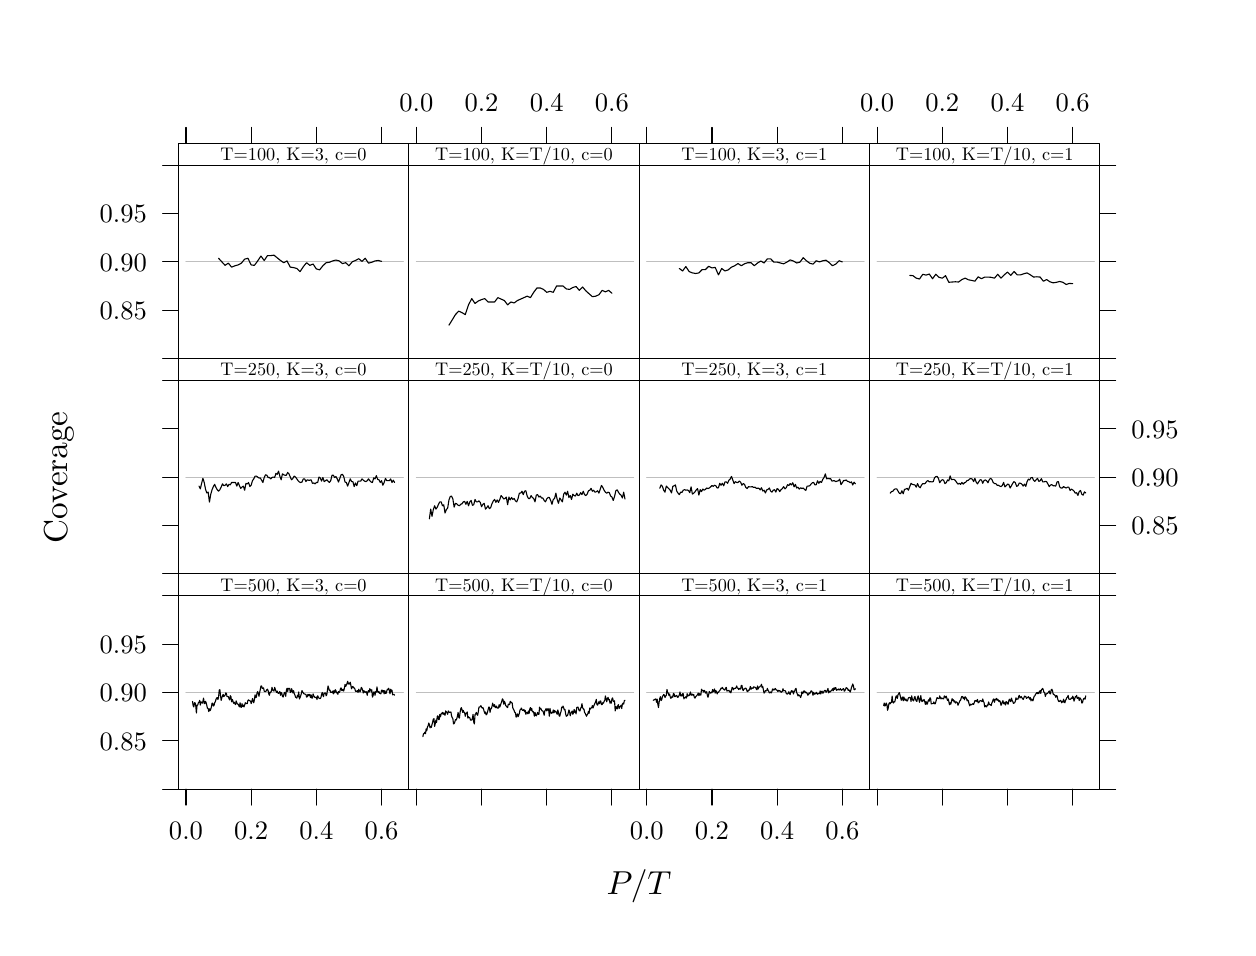
\begin{tikzpicture}[x=1pt,y=1pt]
\definecolor[named]{fillColor}{rgb}{1.00,1.00,1.00}
\path[use as bounding box,fill=fillColor,fill opacity=0.00] (0,0) rectangle (433.62,325.21);
\begin{scope}
\path[clip] (  0.00,  0.00) rectangle (433.62,325.21);

\path[] (  0.00,  0.00) rectangle (433.62,325.21);
\definecolor[named]{drawColor}{rgb}{0.00,0.00,0.00}

\node[text=drawColor,anchor=base,inner sep=0pt, outer sep=0pt, scale=  1.20] at (220.94, 12.05) {$P/T$};
\end{scope}
\begin{scope}
\path[clip] (  0.00,  0.00) rectangle (433.62,325.21);
\definecolor[named]{drawColor}{rgb}{0.00,0.00,0.00}

\node[text=drawColor,rotate= 90.00,anchor=base,inner sep=0pt, outer sep=0pt, scale=  1.20] at ( 14.29,162.76) {Coverage};
\end{scope}
\begin{scope}
\path[clip] (  0.00,  0.00) rectangle (433.62,325.21);
\definecolor[named]{drawColor}{rgb}{0.00,0.00,0.00}

\path[draw=drawColor,line width= 0.4pt,line join=round,line cap=round] ( 54.44, 50.02) -- ( 48.75, 50.02);

\path[draw=drawColor,line width= 0.4pt,line join=round,line cap=round] ( 54.44, 67.48) -- ( 48.75, 67.48);

\path[draw=drawColor,line width= 0.4pt,line join=round,line cap=round] ( 54.44, 84.95) -- ( 48.75, 84.95);

\path[draw=drawColor,line width= 0.4pt,line join=round,line cap=round] ( 54.44,102.42) -- ( 48.75,102.42);

\path[draw=drawColor,line width= 0.4pt,line join=round,line cap=round] ( 54.44,119.88) -- ( 48.75,119.88);

\node[text=drawColor,anchor=base east,inner sep=0pt, outer sep=0pt, scale=  0.96] at ( 43.06, 64.18) {0.85};

\node[text=drawColor,anchor=base east,inner sep=0pt, outer sep=0pt, scale=  0.96] at ( 43.06, 81.64) {0.90};

\node[text=drawColor,anchor=base east,inner sep=0pt, outer sep=0pt, scale=  0.96] at ( 43.06, 99.11) {0.95};
\end{scope}
\begin{scope}
\path[clip] (  0.00,  0.00) rectangle (433.62,325.21);
\definecolor[named]{drawColor}{rgb}{0.00,0.00,0.00}

\path[draw=drawColor,line width= 0.4pt,line join=round,line cap=round] ( 57.20, 50.02) -- ( 57.20, 44.32);

\path[draw=drawColor,line width= 0.4pt,line join=round,line cap=round] ( 80.76, 50.02) -- ( 80.76, 44.32);

\path[draw=drawColor,line width= 0.4pt,line join=round,line cap=round] (104.31, 50.02) -- (104.31, 44.32);

\path[draw=drawColor,line width= 0.4pt,line join=round,line cap=round] (127.87, 50.02) -- (127.87, 44.32);

\node[text=drawColor,anchor=base,inner sep=0pt, outer sep=0pt, scale=  0.96] at ( 57.20, 32.02) {0.0};

\node[text=drawColor,anchor=base,inner sep=0pt, outer sep=0pt, scale=  0.96] at ( 80.76, 32.02) {0.2};

\node[text=drawColor,anchor=base,inner sep=0pt, outer sep=0pt, scale=  0.96] at (104.31, 32.02) {0.4};

\node[text=drawColor,anchor=base,inner sep=0pt, outer sep=0pt, scale=  0.96] at (127.87, 32.02) {0.6};
\end{scope}
\begin{scope}
\path[clip] ( 54.44, 50.02) rectangle (137.69,119.88);
\definecolor[named]{drawColor}{rgb}{0.75,0.75,0.75}

\path[draw=drawColor,line width= 0.4pt,line join=round,line cap=round] ( 57.20, 84.95) --
	(135.72, 84.95);
\definecolor[named]{drawColor}{rgb}{0.00,0.00,0.00}

\path[draw=drawColor,line width= 0.4pt,line join=round,line cap=round] ( 59.56, 81.78) --
	( 59.79, 80.26) --
	( 60.03, 79.76) --
	( 60.26, 81.27) --
	( 60.50, 81.27) --
	( 60.73, 80.26) --
	( 60.97, 77.56) --
	( 61.20, 80.43) --
	( 61.44, 80.43) --
	( 61.68, 81.27) --
	( 61.91, 81.44) --
	( 62.15, 82.12) --
	( 62.38, 80.43) --
	( 62.62, 81.61) --
	( 62.85, 81.44) --
	( 63.09, 81.10) --
	( 63.32, 81.78) --
	( 63.56, 82.96) --
	( 63.80, 80.94) --
	( 64.03, 80.94) --
	( 64.27, 81.78) --
	( 64.50, 81.27) --
	( 64.74, 80.26) --
	( 64.97, 79.25) --
	( 65.21, 79.25) --
	( 65.44, 78.07) --
	( 65.68, 79.08) --
	( 65.92, 78.41) --
	( 66.15, 78.91) --
	( 66.39, 79.76) --
	( 66.62, 81.10) --
	( 66.86, 81.10) --
	( 67.09, 80.09) --
	( 67.33, 80.26) --
	( 67.56, 81.27) --
	( 67.80, 81.61) --
	( 68.04, 82.45) --
	( 68.27, 82.96) --
	( 68.51, 83.13) --
	( 68.74, 82.45) --
	( 68.98, 83.30) --
	( 69.21, 85.83) --
	( 69.45, 85.99) --
	( 69.69, 83.80) --
	( 69.92, 82.12) --
	( 70.16, 83.13) --
	( 70.39, 83.63) --
	( 70.63, 84.31) --
	( 70.86, 83.47) --
	( 71.10, 83.80) --
	( 71.33, 83.97) --
	( 71.57, 84.81) --
	( 71.81, 84.65) --
	( 72.04, 83.47) --
	( 72.28, 83.47) --
	( 72.51, 83.47) --
	( 72.75, 82.79) --
	( 72.98, 82.28) --
	( 73.22, 83.80) --
	( 73.45, 83.47) --
	( 73.69, 81.61) --
	( 73.93, 82.45) --
	( 74.16, 81.95) --
	( 74.40, 81.10) --
	( 74.63, 81.44) --
	( 74.87, 80.94) --
	( 75.10, 80.60) --
	( 75.34, 81.95) --
	( 75.57, 81.27) --
	( 75.81, 80.77) --
	( 76.05, 80.77) --
	( 76.28, 80.26) --
	( 76.52, 79.76) --
	( 76.75, 81.27) --
	( 76.99, 79.76) --
	( 77.22, 79.59) --
	( 77.46, 80.94) --
	( 77.69, 79.92) --
	( 77.93, 80.43) --
	( 78.17, 79.76) --
	( 78.40, 80.43) --
	( 78.64, 81.27) --
	( 78.87, 80.94) --
	( 79.11, 81.10) --
	( 79.34, 80.94) --
	( 79.58, 82.12) --
	( 79.81, 82.28) --
	( 80.05, 82.12) --
	( 80.29, 81.95) --
	( 80.52, 81.95) --
	( 80.76, 80.94) --
	( 80.99, 81.61) --
	( 81.23, 82.79) --
	( 81.46, 81.95) --
	( 81.70, 81.27) --
	( 81.93, 82.45) --
	( 82.17, 84.14) --
	( 82.41, 83.13) --
	( 82.64, 83.30) --
	( 82.88, 84.81) --
	( 83.11, 85.32) --
	( 83.35, 84.65) --
	( 83.58, 83.63) --
	( 83.82, 84.98) --
	( 84.05, 85.99) --
	( 84.29, 87.34) --
	( 84.53, 87.34) --
	( 84.76, 86.50) --
	( 85.00, 86.50) --
	( 85.23, 86.67) --
	( 85.47, 85.49) --
	( 85.70, 85.32) --
	( 85.94, 85.32) --
	( 86.17, 85.49) --
	( 86.41, 85.99) --
	( 86.65, 86.16) --
	( 86.88, 85.66) --
	( 87.12, 84.48) --
	( 87.35, 83.97) --
	( 87.59, 85.15) --
	( 87.82, 84.98) --
	( 88.06, 85.49) --
	( 88.29, 86.84) --
	( 88.53, 85.83) --
	( 88.77, 85.66) --
	( 89.00, 85.49) --
	( 89.24, 86.84) --
	( 89.47, 86.16) --
	( 89.71, 85.49) --
	( 89.94, 84.98) --
	( 90.18, 85.49) --
	( 90.41, 84.81) --
	( 90.65, 84.65) --
	( 90.89, 84.98) --
	( 91.12, 85.32) --
	( 91.36, 83.97) --
	( 91.59, 84.98) --
	( 91.83, 84.65) --
	( 92.06, 83.63) --
	( 92.30, 83.30) --
	( 92.53, 84.14) --
	( 92.77, 84.98) --
	( 93.01, 84.81) --
	( 93.24, 83.63) --
	( 93.48, 85.83) --
	( 93.71, 86.50) --
	( 93.95, 85.32) --
	( 94.18, 86.50) --
	( 94.42, 86.33) --
	( 94.66, 86.50) --
	( 94.89, 84.98) --
	( 95.13, 85.15) --
	( 95.36, 86.33) --
	( 95.60, 85.66) --
	( 95.83, 84.81) --
	( 96.07, 85.66) --
	( 96.30, 84.65) --
	( 96.54, 84.14) --
	( 96.78, 83.30) --
	( 97.01, 83.13) --
	( 97.25, 82.96) --
	( 97.48, 83.97) --
	( 97.72, 83.47) --
	( 97.95, 85.15) --
	( 98.19, 82.62) --
	( 98.42, 83.13) --
	( 98.66, 83.80) --
	( 98.90, 84.65) --
	( 99.13, 85.66) --
	( 99.37, 85.15) --
	( 99.60, 84.81) --
	( 99.84, 84.48) --
	(100.07, 84.48) --
	(100.31, 84.31) --
	(100.54, 84.31) --
	(100.78, 83.30) --
	(101.02, 83.47) --
	(101.25, 84.31) --
	(101.49, 83.80) --
	(101.72, 84.31) --
	(101.96, 84.14) --
	(102.19, 83.13) --
	(102.43, 84.14) --
	(102.66, 82.96) --
	(102.90, 82.96) --
	(103.14, 84.48) --
	(103.37, 83.80) --
	(103.61, 83.47) --
	(103.84, 83.13) --
	(104.08, 83.13) --
	(104.31, 83.30) --
	(104.55, 82.45) --
	(104.78, 83.80) --
	(105.02, 83.30) --
	(105.26, 82.96) --
	(105.49, 82.79) --
	(105.73, 82.79) --
	(105.96, 83.13) --
	(106.20, 84.31) --
	(106.43, 84.98) --
	(106.67, 83.97) --
	(106.90, 83.47) --
	(107.14, 84.81) --
	(107.38, 84.65) --
	(107.61, 84.81) --
	(107.85, 83.80) --
	(108.08, 84.14) --
	(108.32, 85.83) --
	(108.55, 87.34) --
	(108.79, 86.50) --
	(109.02, 85.66) --
	(109.26, 85.83) --
	(109.50, 84.98) --
	(109.73, 85.15) --
	(109.97, 84.98) --
	(110.20, 85.49) --
	(110.44, 84.48) --
	(110.67, 85.66) --
	(110.91, 84.81) --
	(111.14, 85.99) --
	(111.38, 85.66) --
	(111.62, 84.81) --
	(111.85, 84.98) --
	(112.09, 84.31) --
	(112.32, 85.32) --
	(112.56, 84.98) --
	(112.79, 85.32) --
	(113.03, 86.33) --
	(113.26, 86.67) --
	(113.50, 85.66) --
	(113.74, 85.66) --
	(113.97, 86.16) --
	(114.21, 85.49) --
	(114.44, 86.50) --
	(114.68, 87.85) --
	(114.91, 87.17) --
	(115.15, 87.68) --
	(115.38, 88.19) --
	(115.62, 89.03) --
	(115.86, 88.02) --
	(116.09, 88.35) --
	(116.33, 88.02) --
	(116.56, 88.69) --
	(116.80, 87.51) --
	(117.03, 86.33) --
	(117.27, 87.01) --
	(117.51, 87.17) --
	(117.74, 86.67) --
	(117.98, 86.67) --
	(118.21, 86.33) --
	(118.45, 85.49) --
	(118.68, 85.32) --
	(118.92, 85.49) --
	(119.15, 85.66) --
	(119.39, 84.98) --
	(119.63, 86.16) --
	(119.86, 85.66) --
	(120.10, 85.15) --
	(120.33, 85.83) --
	(120.57, 86.84) --
	(120.80, 86.50) --
	(121.04, 85.83) --
	(121.27, 84.81) --
	(121.51, 85.66) --
	(121.75, 85.15) --
	(121.98, 84.98) --
	(122.22, 85.32) --
	(122.45, 85.15) --
	(122.69, 83.97) --
	(122.92, 85.15) --
	(123.16, 85.66) --
	(123.39, 85.15) --
	(123.63, 86.33) --
	(123.87, 85.99) --
	(124.10, 85.32) --
	(124.34, 85.99) --
	(124.57, 83.30) --
	(124.81, 83.80) --
	(125.04, 85.15) --
	(125.28, 85.15) --
	(125.51, 83.97) --
	(125.75, 85.32) --
	(125.99, 85.15) --
	(126.22, 87.01) --
	(126.46, 85.32) --
	(126.69, 84.98) --
	(126.93, 85.32) --
	(127.16, 84.65) --
	(127.40, 84.65) --
	(127.63, 84.48) --
	(127.87, 85.83) --
	(128.11, 85.83) --
	(128.34, 85.15) --
	(128.58, 85.66) --
	(128.81, 84.48) --
	(129.05, 85.66) --
	(129.28, 84.65) --
	(129.52, 84.65) --
	(129.75, 85.49) --
	(129.99, 86.16) --
	(130.23, 85.99) --
	(130.46, 86.50) --
	(130.70, 85.66) --
	(130.93, 84.48) --
	(131.17, 86.16) --
	(131.40, 85.32) --
	(131.64, 85.83) --
	(131.87, 84.14) --
	(132.11, 84.31) --
	(132.35, 84.31) --
	(132.58, 83.97);
\end{scope}
\begin{scope}
\path[clip] (  0.00,  0.00) rectangle (433.62,325.21);
\definecolor[named]{drawColor}{rgb}{0.00,0.00,0.00}

\path[draw=drawColor,line width= 0.4pt,line join=round,line cap=round] ( 54.44, 50.02) rectangle (137.69,119.88);
\end{scope}
\begin{scope}
\path[clip] ( 54.44,119.88) rectangle (137.69,127.83);

\path[] ( 54.44,119.88) rectangle (137.69,127.83);
\definecolor[named]{drawColor}{rgb}{0.00,0.00,0.00}

\node[text=drawColor,anchor=base west,inner sep=0pt, outer sep=0pt, scale=  0.66] at ( 69.67,121.58) {T=500, K=3, c=0};
\end{scope}
\begin{scope}
\path[clip] (  0.00,  0.00) rectangle (433.62,325.21);
\definecolor[named]{drawColor}{rgb}{0.00,0.00,0.00}

\path[draw=drawColor,line width= 0.4pt,line join=round,line cap=round] ( 54.44,119.88) rectangle (137.69,127.83);
\end{scope}
\begin{scope}
\path[clip] (  0.00,  0.00) rectangle (433.62,325.21);
\definecolor[named]{drawColor}{rgb}{0.00,0.00,0.00}

\path[draw=drawColor,line width= 0.4pt,line join=round,line cap=round] (140.45, 50.02) -- (140.45, 44.32);

\path[draw=drawColor,line width= 0.4pt,line join=round,line cap=round] (164.01, 50.02) -- (164.01, 44.32);

\path[draw=drawColor,line width= 0.4pt,line join=round,line cap=round] (187.56, 50.02) -- (187.56, 44.32);

\path[draw=drawColor,line width= 0.4pt,line join=round,line cap=round] (211.12, 50.02) -- (211.12, 44.32);
\end{scope}
\begin{scope}
\path[clip] (137.69, 50.02) rectangle (220.94,119.88);
\definecolor[named]{drawColor}{rgb}{0.75,0.75,0.75}

\path[draw=drawColor,line width= 0.4pt,line join=round,line cap=round] (140.45, 84.95) --
	(218.97, 84.95);
\definecolor[named]{drawColor}{rgb}{0.00,0.00,0.00}

\path[draw=drawColor,line width= 0.4pt,line join=round,line cap=round] (142.80, 69.05) --
	(143.04, 70.10) --
	(143.28, 70.10) --
	(143.51, 70.63) --
	(143.75, 70.10) --
	(143.98, 71.85) --
	(144.22, 71.15) --
	(144.45, 72.55) --
	(144.69, 72.90) --
	(144.92, 73.94) --
	(145.16, 73.42) --
	(145.40, 72.20) --
	(145.63, 72.72) --
	(145.87, 72.37) --
	(146.10, 73.42) --
	(146.34, 74.29) --
	(146.57, 75.34) --
	(146.81, 75.52) --
	(147.05, 72.72) --
	(147.28, 73.77) --
	(147.52, 74.99) --
	(147.75, 74.12) --
	(147.99, 76.22) --
	(148.22, 76.56) --
	(148.46, 75.17) --
	(148.69, 75.17) --
	(148.93, 77.09) --
	(149.17, 76.22) --
	(149.40, 77.26) --
	(149.64, 77.44) --
	(149.87, 77.79) --
	(150.11, 77.09) --
	(150.34, 77.61) --
	(150.58, 77.09) --
	(150.81, 76.74) --
	(151.05, 78.31) --
	(151.29, 77.96) --
	(151.52, 77.61) --
	(151.76, 77.09) --
	(151.99, 78.31) --
	(152.23, 77.96) --
	(152.46, 77.79) --
	(152.70, 77.79) --
	(152.93, 77.96) --
	(153.17, 76.56) --
	(153.41, 75.87) --
	(153.64, 75.52) --
	(153.88, 73.60) --
	(154.11, 73.77) --
	(154.35, 74.29) --
	(154.58, 75.17) --
	(154.82, 74.99) --
	(155.05, 75.52) --
	(155.29, 76.39) --
	(155.53, 77.79) --
	(155.76, 76.04) --
	(156.00, 75.69) --
	(156.23, 77.61) --
	(156.47, 79.01) --
	(156.70, 79.53) --
	(156.94, 78.84) --
	(157.17, 77.79) --
	(157.41, 78.49) --
	(157.65, 77.79) --
	(157.88, 77.79) --
	(158.12, 76.39) --
	(158.35, 77.44) --
	(158.59, 77.44) --
	(158.82, 77.96) --
	(159.06, 75.69) --
	(159.29, 76.22) --
	(159.53, 75.87) --
	(159.77, 75.87) --
	(160.00, 74.99) --
	(160.24, 74.99) --
	(160.47, 74.99) --
	(160.71, 75.69) --
	(160.94, 77.09) --
	(161.18, 74.29) --
	(161.41, 73.60) --
	(161.65, 76.91) --
	(161.89, 77.26) --
	(162.12, 77.79) --
	(162.36, 77.09) --
	(162.59, 76.74) --
	(162.83, 77.96) --
	(163.06, 79.71) --
	(163.30, 79.71) --
	(163.53, 79.88) --
	(163.77, 80.23) --
	(164.01, 79.71) --
	(164.24, 79.36) --
	(164.48, 79.53) --
	(164.71, 79.01) --
	(164.95, 78.14) --
	(165.18, 77.44) --
	(165.42, 77.96) --
	(165.65, 76.91) --
	(165.89, 77.09) --
	(166.13, 77.79) --
	(166.36, 78.66) --
	(166.60, 79.71) --
	(166.83, 79.71) --
	(167.07, 77.79) --
	(167.30, 79.01) --
	(167.54, 79.18) --
	(167.77, 79.88) --
	(168.01, 81.11) --
	(168.25, 80.41) --
	(168.48, 79.88) --
	(168.72, 80.58) --
	(168.95, 79.53) --
	(169.19, 79.53) --
	(169.42, 80.06) --
	(169.66, 79.36) --
	(169.90, 79.36) --
	(170.13, 79.36) --
	(170.37, 80.58) --
	(170.60, 79.71) --
	(170.84, 80.41) --
	(171.07, 81.11) --
	(171.31, 81.80) --
	(171.54, 82.68) --
	(171.78, 82.33) --
	(172.02, 80.76) --
	(172.25, 81.80) --
	(172.49, 81.28) --
	(172.72, 80.23) --
	(172.96, 80.06) --
	(173.19, 79.71) --
	(173.43, 79.53) --
	(173.66, 80.76) --
	(173.90, 80.76) --
	(174.14, 80.58) --
	(174.37, 81.80) --
	(174.61, 81.28) --
	(174.84, 81.46) --
	(175.08, 81.11) --
	(175.31, 79.36) --
	(175.55, 78.84) --
	(175.78, 78.49) --
	(176.02, 77.79) --
	(176.26, 77.61) --
	(176.49, 76.04) --
	(176.73, 76.74) --
	(176.96, 77.26) --
	(177.20, 76.22) --
	(177.43, 76.74) --
	(177.67, 77.44) --
	(177.90, 78.66) --
	(178.14, 78.84) --
	(178.38, 79.36) --
	(178.61, 78.84) --
	(178.85, 78.49) --
	(179.08, 78.49) --
	(179.32, 78.84) --
	(179.55, 77.96) --
	(179.79, 78.49) --
	(180.02, 77.09) --
	(180.26, 77.79) --
	(180.50, 77.79) --
	(180.73, 77.26) --
	(180.97, 78.31) --
	(181.20, 77.44) --
	(181.44, 79.01) --
	(181.67, 79.53) --
	(181.91, 78.49) --
	(182.14, 79.18) --
	(182.38, 77.96) --
	(182.62, 78.14) --
	(182.85, 77.79) --
	(183.09, 76.39) --
	(183.32, 77.79) --
	(183.56, 76.74) --
	(183.79, 76.56) --
	(184.03, 77.09) --
	(184.26, 77.79) --
	(184.50, 77.09) --
	(184.74, 77.09) --
	(184.97, 79.71) --
	(185.21, 79.01) --
	(185.44, 79.18) --
	(185.68, 78.66) --
	(185.91, 78.31) --
	(186.15, 78.31) --
	(186.38, 77.79) --
	(186.62, 76.74) --
	(186.86, 78.31) --
	(187.09, 78.66) --
	(187.33, 79.18) --
	(187.56, 78.31) --
	(187.80, 78.66) --
	(188.03, 79.18) --
	(188.27, 78.66) --
	(188.50, 76.39) --
	(188.74, 79.18) --
	(188.98, 77.79) --
	(189.21, 77.44) --
	(189.45, 77.79) --
	(189.68, 77.61) --
	(189.92, 78.66) --
	(190.15, 77.61) --
	(190.39, 78.49) --
	(190.62, 77.96) --
	(190.86, 78.14) --
	(191.10, 77.61) --
	(191.33, 77.09) --
	(191.57, 78.66) --
	(191.80, 77.79) --
	(192.04, 76.56) --
	(192.27, 76.39) --
	(192.51, 77.44) --
	(192.74, 78.14) --
	(192.98, 79.71) --
	(193.22, 79.53) --
	(193.45, 80.06) --
	(193.69, 79.36) --
	(193.92, 78.66) --
	(194.16, 78.84) --
	(194.39, 77.26) --
	(194.63, 76.39) --
	(194.87, 76.56) --
	(195.10, 76.74) --
	(195.34, 77.61) --
	(195.57, 78.66) --
	(195.81, 78.14) --
	(196.04, 76.56) --
	(196.28, 77.44) --
	(196.51, 77.79) --
	(196.75, 78.31) --
	(196.99, 77.09) --
	(197.22, 77.61) --
	(197.46, 78.84) --
	(197.69, 77.79) --
	(197.93, 78.31) --
	(198.16, 77.26) --
	(198.40, 79.53) --
	(198.63, 79.71) --
	(198.87, 79.71) --
	(199.11, 78.84) --
	(199.34, 78.31) --
	(199.58, 78.31) --
	(199.81, 79.36) --
	(200.05, 79.53) --
	(200.28, 80.93) --
	(200.52, 79.53) --
	(200.75, 79.01) --
	(200.99, 79.01) --
	(201.23, 77.79) --
	(201.46, 77.44) --
	(201.70, 76.91) --
	(201.93, 76.39) --
	(202.17, 76.91) --
	(202.40, 77.26) --
	(202.64, 78.14) --
	(202.87, 77.44) --
	(203.11, 79.36) --
	(203.35, 79.01) --
	(203.58, 79.36) --
	(203.82, 79.53) --
	(204.05, 80.23) --
	(204.29, 79.36) --
	(204.52, 80.06) --
	(204.76, 80.58) --
	(204.99, 81.11) --
	(205.23, 81.63) --
	(205.47, 82.50) --
	(205.70, 80.58) --
	(205.94, 80.41) --
	(206.17, 80.93) --
	(206.41, 81.63) --
	(206.64, 80.93) --
	(206.88, 81.98) --
	(207.11, 81.80) --
	(207.35, 80.58) --
	(207.59, 80.58) --
	(207.82, 81.28) --
	(208.06, 81.11) --
	(208.29, 81.80) --
	(208.53, 82.15) --
	(208.76, 83.73) --
	(209.00, 82.68) --
	(209.23, 81.63) --
	(209.47, 82.68) --
	(209.71, 83.20) --
	(209.94, 82.33) --
	(210.18, 82.50) --
	(210.41, 81.11) --
	(210.65, 81.80) --
	(210.88, 81.11) --
	(211.12, 82.68) --
	(211.35, 83.03) --
	(211.59, 81.98) --
	(211.83, 81.63) --
	(212.06, 81.98) --
	(212.30, 78.31) --
	(212.53, 79.88) --
	(212.77, 79.71) --
	(213.00, 79.01) --
	(213.24, 80.23) --
	(213.47, 80.58) --
	(213.71, 79.18) --
	(213.95, 79.88) --
	(214.18, 79.88) --
	(214.42, 80.41) --
	(214.65, 79.18) --
	(214.89, 80.76) --
	(215.12, 81.11) --
	(215.36, 80.76) --
	(215.59, 81.98) --
	(215.83, 82.15);
\end{scope}
\begin{scope}
\path[clip] (  0.00,  0.00) rectangle (433.62,325.21);
\definecolor[named]{drawColor}{rgb}{0.00,0.00,0.00}

\path[draw=drawColor,line width= 0.4pt,line join=round,line cap=round] (137.69, 50.02) rectangle (220.94,119.88);
\end{scope}
\begin{scope}
\path[clip] (137.69,119.88) rectangle (220.94,127.83);

\path[] (137.69,119.88) rectangle (220.94,127.83);
\definecolor[named]{drawColor}{rgb}{0.00,0.00,0.00}

\node[text=drawColor,anchor=base west,inner sep=0pt, outer sep=0pt, scale=  0.66] at (147.24,121.58) {T=500, K=T/10, c=0};
\end{scope}
\begin{scope}
\path[clip] (  0.00,  0.00) rectangle (433.62,325.21);
\definecolor[named]{drawColor}{rgb}{0.00,0.00,0.00}

\path[draw=drawColor,line width= 0.4pt,line join=round,line cap=round] (137.69,119.88) rectangle (220.94,127.83);
\end{scope}
\begin{scope}
\path[clip] (  0.00,  0.00) rectangle (433.62,325.21);
\definecolor[named]{drawColor}{rgb}{0.00,0.00,0.00}

\path[draw=drawColor,line width= 0.4pt,line join=round,line cap=round] (223.70, 50.02) -- (223.70, 44.32);

\path[draw=drawColor,line width= 0.4pt,line join=round,line cap=round] (247.26, 50.02) -- (247.26, 44.32);

\path[draw=drawColor,line width= 0.4pt,line join=round,line cap=round] (270.81, 50.02) -- (270.81, 44.32);

\path[draw=drawColor,line width= 0.4pt,line join=round,line cap=round] (294.37, 50.02) -- (294.37, 44.32);

\node[text=drawColor,anchor=base,inner sep=0pt, outer sep=0pt, scale=  0.96] at (223.70, 32.02) {0.0};

\node[text=drawColor,anchor=base,inner sep=0pt, outer sep=0pt, scale=  0.96] at (247.26, 32.02) {0.2};

\node[text=drawColor,anchor=base,inner sep=0pt, outer sep=0pt, scale=  0.96] at (270.81, 32.02) {0.4};

\node[text=drawColor,anchor=base,inner sep=0pt, outer sep=0pt, scale=  0.96] at (294.37, 32.02) {0.6};
\end{scope}
\begin{scope}
\path[clip] (220.94, 50.02) rectangle (304.19,119.88);
\definecolor[named]{drawColor}{rgb}{0.75,0.75,0.75}

\path[draw=drawColor,line width= 0.4pt,line join=round,line cap=round] (223.70, 84.95) --
	(302.22, 84.95);
\definecolor[named]{drawColor}{rgb}{0.00,0.00,0.00}

\path[draw=drawColor,line width= 0.4pt,line join=round,line cap=round] (226.05, 82.15) --
	(226.29, 82.25) --
	(226.53, 82.45) --
	(226.76, 82.55) --
	(227.00, 82.65) --
	(227.23, 81.46) --
	(227.47, 82.55) --
	(227.70, 80.76) --
	(227.94, 79.56) --
	(228.17, 81.46) --
	(228.41, 82.85) --
	(228.65, 83.45) --
	(228.88, 82.05) --
	(229.12, 82.35) --
	(229.35, 83.45) --
	(229.59, 83.85) --
	(229.82, 84.25) --
	(230.06, 84.05) --
	(230.29, 83.15) --
	(230.53, 83.65) --
	(230.77, 83.95) --
	(231.00, 86.05) --
	(231.24, 85.05) --
	(231.47, 84.75) --
	(231.71, 83.95) --
	(231.94, 84.45) --
	(232.18, 83.45) --
	(232.41, 82.85) --
	(232.65, 83.15) --
	(232.89, 83.65) --
	(233.12, 83.25) --
	(233.36, 84.65) --
	(233.59, 84.45) --
	(233.83, 83.45) --
	(234.06, 83.55) --
	(234.30, 83.75) --
	(234.53, 83.95) --
	(234.77, 83.25) --
	(235.01, 83.25) --
	(235.24, 83.65) --
	(235.48, 84.05) --
	(235.71, 85.15) --
	(235.95, 83.75) --
	(236.18, 84.15) --
	(236.42, 83.65) --
	(236.65, 84.55) --
	(236.89, 84.55) --
	(237.13, 82.65) --
	(237.36, 83.15) --
	(237.60, 83.05) --
	(237.83, 83.45) --
	(238.07, 82.95) --
	(238.30, 84.55) --
	(238.54, 83.65) --
	(238.77, 84.05) --
	(239.01, 83.85) --
	(239.25, 84.45) --
	(239.48, 85.15) --
	(239.72, 83.95) --
	(239.95, 84.35) --
	(240.19, 84.35) --
	(240.42, 83.95) --
	(240.66, 84.25) --
	(240.89, 83.25) --
	(241.13, 82.95) --
	(241.37, 83.45) --
	(241.60, 83.65) --
	(241.84, 83.95) --
	(242.07, 84.25) --
	(242.31, 84.75) --
	(242.54, 83.85) --
	(242.78, 84.55) --
	(243.01, 84.15) --
	(243.25, 84.05) --
	(243.49, 86.15) --
	(243.72, 85.75) --
	(243.96, 85.75) --
	(244.19, 85.15) --
	(244.43, 85.75) --
	(244.66, 85.55) --
	(244.90, 84.75) --
	(245.13, 85.05) --
	(245.37, 85.25) --
	(245.61, 83.85) --
	(245.84, 83.25) --
	(246.08, 84.25) --
	(246.31, 85.35) --
	(246.55, 84.85) --
	(246.78, 84.75) --
	(247.02, 85.05) --
	(247.26, 84.85) --
	(247.49, 86.05) --
	(247.73, 85.25) --
	(247.96, 85.65) --
	(248.20, 86.25) --
	(248.43, 84.75) --
	(248.67, 85.65) --
	(248.90, 85.35) --
	(249.14, 84.45) --
	(249.38, 85.05) --
	(249.61, 85.05) --
	(249.85, 85.45) --
	(250.08, 85.65) --
	(250.32, 86.05) --
	(250.55, 86.55) --
	(250.79, 86.35) --
	(251.02, 86.85) --
	(251.26, 86.35) --
	(251.50, 86.15) --
	(251.73, 85.85) --
	(251.97, 85.95) --
	(252.20, 86.55) --
	(252.44, 86.85) --
	(252.67, 85.45) --
	(252.91, 85.65) --
	(253.14, 85.65) --
	(253.38, 85.75) --
	(253.62, 85.15) --
	(253.85, 85.45) --
	(254.09, 84.85) --
	(254.32, 85.75) --
	(254.56, 86.85) --
	(254.79, 86.65) --
	(255.03, 85.95) --
	(255.26, 86.45) --
	(255.50, 86.45) --
	(255.74, 86.45) --
	(255.97, 86.75) --
	(256.21, 87.34) --
	(256.44, 86.55) --
	(256.68, 86.55) --
	(256.91, 86.05) --
	(257.15, 86.45) --
	(257.38, 86.25) --
	(257.62, 86.25) --
	(257.86, 87.54) --
	(258.09, 87.54) --
	(258.33, 86.15) --
	(258.56, 85.65) --
	(258.80, 86.25) --
	(259.03, 86.25) --
	(259.27, 86.55) --
	(259.50, 86.55) --
	(259.74, 86.15) --
	(259.98, 85.35) --
	(260.21, 85.25) --
	(260.45, 85.85) --
	(260.68, 85.75) --
	(260.92, 86.35) --
	(261.15, 87.14) --
	(261.39, 86.15) --
	(261.62, 86.65) --
	(261.86, 86.55) --
	(262.10, 86.45) --
	(262.33, 87.04) --
	(262.57, 86.94) --
	(262.80, 86.85) --
	(263.04, 86.75) --
	(263.27, 86.25) --
	(263.51, 85.95) --
	(263.74, 87.34) --
	(263.98, 86.25) --
	(264.22, 86.94) --
	(264.45, 86.94) --
	(264.69, 87.24) --
	(264.92, 87.34) --
	(265.16, 87.94) --
	(265.39, 86.75) --
	(265.63, 87.14) --
	(265.86, 85.85) --
	(266.10, 84.75) --
	(266.34, 85.05) --
	(266.57, 85.65) --
	(266.81, 85.55) --
	(267.04, 85.55) --
	(267.28, 86.45) --
	(267.51, 85.85) --
	(267.75, 85.45) --
	(267.98, 84.85) --
	(268.22, 84.95) --
	(268.46, 85.15) --
	(268.69, 84.85) --
	(268.93, 85.35) --
	(269.16, 86.25) --
	(269.40, 85.85) --
	(269.63, 86.15) --
	(269.87, 85.95) --
	(270.11, 86.45) --
	(270.34, 86.15) --
	(270.58, 85.85) --
	(270.81, 85.85) --
	(271.05, 85.35) --
	(271.28, 85.75) --
	(271.52, 85.45) --
	(271.75, 85.65) --
	(271.99, 85.45) --
	(272.23, 85.05) --
	(272.46, 85.15) --
	(272.70, 85.45) --
	(272.93, 86.35) --
	(273.17, 85.55) --
	(273.40, 85.65) --
	(273.64, 85.65) --
	(273.87, 85.45) --
	(274.11, 84.65) --
	(274.35, 84.45) --
	(274.58, 84.45) --
	(274.82, 84.75) --
	(275.05, 85.25) --
	(275.29, 84.55) --
	(275.52, 84.25) --
	(275.76, 85.15) --
	(275.99, 85.65) --
	(276.23, 85.15) --
	(276.47, 85.55) --
	(276.70, 84.45) --
	(276.94, 85.25) --
	(277.17, 85.55) --
	(277.41, 86.25) --
	(277.64, 86.45) --
	(277.88, 84.95) --
	(278.11, 84.45) --
	(278.35, 83.75) --
	(278.59, 84.15) --
	(278.82, 83.85) --
	(279.06, 83.75) --
	(279.29, 83.15) --
	(279.53, 83.85) --
	(279.76, 85.25) --
	(280.00, 84.55) --
	(280.23, 84.85) --
	(280.47, 85.55) --
	(280.71, 85.55) --
	(280.94, 84.85) --
	(281.18, 85.15) --
	(281.41, 84.95) --
	(281.65, 84.65) --
	(281.88, 84.05) --
	(282.12, 84.15) --
	(282.35, 84.85) --
	(282.59, 84.55) --
	(282.83, 85.05) --
	(283.06, 85.55) --
	(283.30, 85.55) --
	(283.53, 85.05) --
	(283.77, 83.95) --
	(284.00, 85.05) --
	(284.24, 84.35) --
	(284.47, 84.55) --
	(284.71, 84.45) --
	(284.95, 85.05) --
	(285.18, 84.75) --
	(285.42, 84.35) --
	(285.65, 84.55) --
	(285.89, 84.65) --
	(286.12, 84.55) --
	(286.36, 85.55) --
	(286.59, 84.45) --
	(286.83, 85.25) --
	(287.07, 85.45) --
	(287.30, 84.75) --
	(287.54, 84.85) --
	(287.77, 85.45) --
	(288.01, 85.75) --
	(288.24, 85.75) --
	(288.48, 85.05) --
	(288.71, 85.35) --
	(288.95, 85.75) --
	(289.19, 86.45) --
	(289.42, 84.85) --
	(289.66, 85.45) --
	(289.89, 85.15) --
	(290.13, 85.35) --
	(290.36, 85.65) --
	(290.60, 85.85) --
	(290.83, 86.35) --
	(291.07, 85.55) --
	(291.31, 86.65) --
	(291.54, 86.05) --
	(291.78, 86.75) --
	(292.01, 86.75) --
	(292.25, 85.75) --
	(292.48, 86.05) --
	(292.72, 85.95) --
	(292.96, 86.25) --
	(293.19, 85.85) --
	(293.43, 86.05) --
	(293.66, 86.35) --
	(293.90, 85.95) --
	(294.13, 85.75) --
	(294.37, 86.05) --
	(294.60, 86.25) --
	(294.84, 86.35) --
	(295.08, 85.45) --
	(295.31, 85.65) --
	(295.55, 86.15) --
	(295.78, 86.75) --
	(296.02, 86.55) --
	(296.25, 86.45) --
	(296.49, 85.75) --
	(296.72, 85.95) --
	(296.96, 85.65) --
	(297.20, 85.15) --
	(297.43, 85.75) --
	(297.67, 86.75) --
	(297.90, 87.34) --
	(298.14, 88.04) --
	(298.37, 87.44) --
	(298.61, 86.05) --
	(298.84, 85.95) --
	(299.08, 86.35);
\end{scope}
\begin{scope}
\path[clip] (  0.00,  0.00) rectangle (433.62,325.21);
\definecolor[named]{drawColor}{rgb}{0.00,0.00,0.00}

\path[draw=drawColor,line width= 0.4pt,line join=round,line cap=round] (220.94, 50.02) rectangle (304.19,119.88);
\end{scope}
\begin{scope}
\path[clip] (220.94,119.88) rectangle (304.19,127.83);

\path[] (220.94,119.88) rectangle (304.19,127.83);
\definecolor[named]{drawColor}{rgb}{0.00,0.00,0.00}

\node[text=drawColor,anchor=base west,inner sep=0pt, outer sep=0pt, scale=  0.66] at (236.17,121.58) {T=500, K=3, c=1};
\end{scope}
\begin{scope}
\path[clip] (  0.00,  0.00) rectangle (433.62,325.21);
\definecolor[named]{drawColor}{rgb}{0.00,0.00,0.00}

\path[draw=drawColor,line width= 0.4pt,line join=round,line cap=round] (220.94,119.88) rectangle (304.19,127.83);
\end{scope}
\begin{scope}
\path[clip] (  0.00,  0.00) rectangle (433.62,325.21);
\definecolor[named]{drawColor}{rgb}{0.00,0.00,0.00}

\path[draw=drawColor,line width= 0.4pt,line join=round,line cap=round] (306.95, 50.02) -- (306.95, 44.32);

\path[draw=drawColor,line width= 0.4pt,line join=round,line cap=round] (330.50, 50.02) -- (330.50, 44.32);

\path[draw=drawColor,line width= 0.4pt,line join=round,line cap=round] (354.06, 50.02) -- (354.06, 44.32);

\path[draw=drawColor,line width= 0.4pt,line join=round,line cap=round] (377.62, 50.02) -- (377.62, 44.32);

\path[draw=drawColor,line width= 0.4pt,line join=round,line cap=round] (387.44, 50.02) -- (393.13, 50.02);

\path[draw=drawColor,line width= 0.4pt,line join=round,line cap=round] (387.44, 67.48) -- (393.13, 67.48);

\path[draw=drawColor,line width= 0.4pt,line join=round,line cap=round] (387.44, 84.95) -- (393.13, 84.95);

\path[draw=drawColor,line width= 0.4pt,line join=round,line cap=round] (387.44,102.42) -- (393.13,102.42);

\path[draw=drawColor,line width= 0.4pt,line join=round,line cap=round] (387.44,119.88) -- (393.13,119.88);
\end{scope}
\begin{scope}
\path[clip] (304.19, 50.02) rectangle (387.44,119.88);
\definecolor[named]{drawColor}{rgb}{0.75,0.75,0.75}

\path[draw=drawColor,line width= 0.4pt,line join=round,line cap=round] (306.95, 84.95) --
	(385.47, 84.95);
\definecolor[named]{drawColor}{rgb}{0.00,0.00,0.00}

\path[draw=drawColor,line width= 0.4pt,line join=round,line cap=round] (309.30, 80.26) --
	(309.54, 81.16) --
	(309.77, 80.06) --
	(310.01, 80.46) --
	(310.25, 81.16) --
	(310.48, 80.56) --
	(310.72, 78.56) --
	(310.95, 79.36) --
	(311.19, 80.86) --
	(311.42, 81.26) --
	(311.66, 80.86) --
	(311.89, 81.36) --
	(312.13, 81.36) --
	(312.37, 83.65) --
	(312.60, 81.66) --
	(312.84, 81.16) --
	(313.07, 81.66) --
	(313.31, 81.56) --
	(313.54, 82.55) --
	(313.78, 83.65) --
	(314.01, 83.75) --
	(314.25, 82.85) --
	(314.49, 84.15) --
	(314.72, 84.45) --
	(314.96, 84.95) --
	(315.19, 84.15) --
	(315.43, 83.25) --
	(315.66, 82.15) --
	(315.90, 82.95) --
	(316.13, 83.35) --
	(316.37, 81.95) --
	(316.61, 83.35) --
	(316.84, 82.55) --
	(317.08, 82.15) --
	(317.31, 82.65) --
	(317.55, 82.15) --
	(317.78, 81.85) --
	(318.02, 82.25) --
	(318.25, 83.05) --
	(318.49, 83.15) --
	(318.73, 83.15) --
	(318.96, 83.05) --
	(319.20, 81.75) --
	(319.43, 83.75) --
	(319.67, 82.55) --
	(319.90, 82.15) --
	(320.14, 81.95) --
	(320.37, 83.05) --
	(320.61, 83.55) --
	(320.85, 82.45) --
	(321.08, 81.95) --
	(321.32, 81.75) --
	(321.55, 83.15) --
	(321.79, 83.75) --
	(322.02, 82.55) --
	(322.26, 81.46) --
	(322.50, 82.65) --
	(322.73, 83.85) --
	(322.97, 82.05) --
	(323.20, 81.66) --
	(323.44, 82.25) --
	(323.67, 81.95) --
	(323.91, 82.45) --
	(324.14, 81.75) --
	(324.38, 80.66) --
	(324.62, 81.75) --
	(324.85, 80.76) --
	(325.09, 80.76) --
	(325.32, 81.75) --
	(325.56, 82.35) --
	(325.79, 81.85) --
	(326.03, 83.05) --
	(326.26, 82.95) --
	(326.50, 80.86) --
	(326.74, 80.96) --
	(326.97, 80.96) --
	(327.21, 80.96) --
	(327.44, 81.56) --
	(327.68, 80.96) --
	(327.91, 80.86) --
	(328.15, 81.56) --
	(328.38, 82.45) --
	(328.62, 83.15) --
	(328.86, 82.85) --
	(329.09, 82.85) --
	(329.33, 82.75) --
	(329.56, 83.75) --
	(329.80, 83.05) --
	(330.03, 82.65) --
	(330.27, 83.05) --
	(330.50, 82.75) --
	(330.74, 82.75) --
	(330.98, 82.65) --
	(331.21, 83.75) --
	(331.45, 83.45) --
	(331.68, 83.05) --
	(331.92, 83.65) --
	(332.15, 82.85) --
	(332.39, 82.05) --
	(332.62, 82.65) --
	(332.86, 81.75) --
	(333.10, 80.56) --
	(333.33, 81.26) --
	(333.57, 80.76) --
	(333.80, 81.75) --
	(334.04, 82.75) --
	(334.27, 82.05) --
	(334.51, 82.35) --
	(334.74, 81.56) --
	(334.98, 81.95) --
	(335.22, 81.16) --
	(335.45, 81.56) --
	(335.69, 81.56) --
	(335.92, 81.26) --
	(336.16, 80.36) --
	(336.39, 80.96) --
	(336.63, 81.46) --
	(336.86, 82.05) --
	(337.10, 82.15) --
	(337.34, 83.05) --
	(337.57, 83.55) --
	(337.81, 83.45) --
	(338.04, 82.85) --
	(338.28, 83.25) --
	(338.51, 82.35) --
	(338.75, 83.45) --
	(338.98, 83.05) --
	(339.22, 82.95) --
	(339.46, 81.95) --
	(339.69, 82.25) --
	(339.93, 81.95) --
	(340.16, 80.86) --
	(340.40, 80.16) --
	(340.63, 80.76) --
	(340.87, 80.56) --
	(341.10, 80.56) --
	(341.34, 80.76) --
	(341.58, 80.96) --
	(341.81, 80.66) --
	(342.05, 81.36) --
	(342.28, 82.05) --
	(342.52, 81.85) --
	(342.75, 82.15) --
	(342.99, 81.66) --
	(343.22, 82.45) --
	(343.46, 81.26) --
	(343.70, 81.36) --
	(343.93, 81.75) --
	(344.17, 82.05) --
	(344.40, 82.05) --
	(344.64, 81.85) --
	(344.87, 81.66) --
	(345.11, 82.65) --
	(345.35, 81.75) --
	(345.58, 81.36) --
	(345.82, 79.76) --
	(346.05, 80.26) --
	(346.29, 79.96) --
	(346.52, 79.76) --
	(346.76, 80.46) --
	(346.99, 80.36) --
	(347.23, 81.56) --
	(347.47, 80.76) --
	(347.70, 80.56) --
	(347.94, 80.56) --
	(348.17, 80.26) --
	(348.41, 81.26) --
	(348.64, 81.66) --
	(348.88, 82.45) --
	(349.11, 82.65) --
	(349.35, 81.46) --
	(349.59, 82.45) --
	(349.82, 82.45) --
	(350.06, 82.85) --
	(350.29, 82.15) --
	(350.53, 82.55) --
	(350.76, 82.15) --
	(351.00, 81.66) --
	(351.23, 82.05) --
	(351.47, 81.46) --
	(351.71, 80.36) --
	(351.94, 80.76) --
	(352.18, 81.56) --
	(352.41, 82.05) --
	(352.65, 80.96) --
	(352.88, 80.86) --
	(353.12, 81.46) --
	(353.35, 80.46) --
	(353.59, 81.66) --
	(353.83, 81.56) --
	(354.06, 80.96) --
	(354.30, 80.76) --
	(354.53, 82.05) --
	(354.77, 82.55) --
	(355.00, 81.95) --
	(355.24, 81.66) --
	(355.47, 82.95) --
	(355.71, 82.15) --
	(355.95, 81.75) --
	(356.18, 81.06) --
	(356.42, 81.16) --
	(356.65, 81.26) --
	(356.89, 81.85) --
	(357.12, 83.05) --
	(357.36, 82.45) --
	(357.59, 82.65) --
	(357.83, 82.55) --
	(358.07, 83.45) --
	(358.30, 83.95) --
	(358.54, 83.05) --
	(358.77, 83.15) --
	(359.01, 83.55) --
	(359.24, 83.05) --
	(359.48, 82.85) --
	(359.71, 82.45) --
	(359.95, 82.95) --
	(360.19, 83.65) --
	(360.42, 83.45) --
	(360.66, 83.55) --
	(360.89, 82.85) --
	(361.13, 83.05) --
	(361.36, 83.15) --
	(361.60, 83.45) --
	(361.83, 83.15) --
	(362.07, 82.55) --
	(362.31, 83.15) --
	(362.54, 81.95) --
	(362.78, 82.55) --
	(363.01, 82.35) --
	(363.25, 81.95) --
	(363.48, 82.95) --
	(363.72, 83.65) --
	(363.95, 83.75) --
	(364.19, 84.45) --
	(364.43, 84.55) --
	(364.66, 84.95) --
	(364.90, 84.55) --
	(365.13, 85.05) --
	(365.37, 84.55) --
	(365.60, 85.25) --
	(365.84, 85.65) --
	(366.07, 84.65) --
	(366.31, 86.05) --
	(366.55, 86.15) --
	(366.78, 86.45) --
	(367.02, 85.85) --
	(367.25, 84.95) --
	(367.49, 84.95) --
	(367.72, 83.55) --
	(367.96, 84.35) --
	(368.19, 84.55) --
	(368.43, 84.55) --
	(368.67, 84.85) --
	(368.90, 85.15) --
	(369.14, 85.55) --
	(369.37, 84.55) --
	(369.61, 84.45) --
	(369.84, 85.95) --
	(370.08, 86.15) --
	(370.32, 85.65) --
	(370.55, 84.35) --
	(370.79, 84.35) --
	(371.02, 84.05) --
	(371.26, 83.95) --
	(371.49, 83.25) --
	(371.73, 83.85) --
	(371.96, 83.75) --
	(372.20, 82.65) --
	(372.44, 81.95) --
	(372.67, 81.66) --
	(372.91, 81.85) --
	(373.14, 82.15) --
	(373.38, 81.95) --
	(373.61, 81.26) --
	(373.85, 81.75) --
	(374.08, 81.46) --
	(374.32, 82.55) --
	(374.56, 81.56) --
	(374.79, 81.26) --
	(375.03, 82.15) --
	(375.26, 82.55) --
	(375.50, 83.15) --
	(375.73, 83.25) --
	(375.97, 83.95) --
	(376.20, 82.65) --
	(376.44, 82.55) --
	(376.68, 82.45) --
	(376.91, 82.65) --
	(377.15, 83.05) --
	(377.38, 82.75) --
	(377.62, 83.65) --
	(377.85, 83.15) --
	(378.09, 81.85) --
	(378.32, 82.55) --
	(378.56, 83.45) --
	(378.80, 83.35) --
	(379.03, 83.95) --
	(379.27, 82.85) --
	(379.50, 82.95) --
	(379.74, 83.25) --
	(379.97, 82.05) --
	(380.21, 83.05) --
	(380.44, 82.75) --
	(380.68, 82.35) --
	(380.92, 81.16) --
	(381.15, 81.26) --
	(381.39, 82.35) --
	(381.62, 82.75) --
	(381.86, 82.95) --
	(382.09, 82.55) --
	(382.33, 83.75);
\end{scope}
\begin{scope}
\path[clip] (  0.00,  0.00) rectangle (433.62,325.21);
\definecolor[named]{drawColor}{rgb}{0.00,0.00,0.00}

\path[draw=drawColor,line width= 0.4pt,line join=round,line cap=round] (304.19, 50.02) rectangle (387.44,119.88);
\end{scope}
\begin{scope}
\path[clip] (304.19,119.88) rectangle (387.44,127.83);

\path[] (304.19,119.88) rectangle (387.44,127.83);
\definecolor[named]{drawColor}{rgb}{0.00,0.00,0.00}

\node[text=drawColor,anchor=base west,inner sep=0pt, outer sep=0pt, scale=  0.66] at (313.74,121.58) {T=500, K=T/10, c=1};
\end{scope}
\begin{scope}
\path[clip] (  0.00,  0.00) rectangle (433.62,325.21);
\definecolor[named]{drawColor}{rgb}{0.00,0.00,0.00}

\path[draw=drawColor,line width= 0.4pt,line join=round,line cap=round] (304.19,119.88) rectangle (387.44,127.83);
\end{scope}
\begin{scope}
\path[clip] (  0.00,  0.00) rectangle (433.62,325.21);
\definecolor[named]{drawColor}{rgb}{0.00,0.00,0.00}

\path[draw=drawColor,line width= 0.4pt,line join=round,line cap=round] ( 54.44,127.83) -- ( 48.75,127.83);

\path[draw=drawColor,line width= 0.4pt,line join=round,line cap=round] ( 54.44,145.30) -- ( 48.75,145.30);

\path[draw=drawColor,line width= 0.4pt,line join=round,line cap=round] ( 54.44,162.76) -- ( 48.75,162.76);

\path[draw=drawColor,line width= 0.4pt,line join=round,line cap=round] ( 54.44,180.23) -- ( 48.75,180.23);

\path[draw=drawColor,line width= 0.4pt,line join=round,line cap=round] ( 54.44,197.70) -- ( 48.75,197.70);
\end{scope}
\begin{scope}
\path[clip] ( 54.44,127.83) rectangle (137.69,197.70);
\definecolor[named]{drawColor}{rgb}{0.75,0.75,0.75}

\path[draw=drawColor,line width= 0.4pt,line join=round,line cap=round] ( 57.20,162.76) --
	(135.72,162.76);
\definecolor[named]{drawColor}{rgb}{0.00,0.00,0.00}

\path[draw=drawColor,line width= 0.4pt,line join=round,line cap=round] ( 61.91,159.54) --
	( 62.38,158.55) --
	( 62.85,160.53) --
	( 63.32,162.34) --
	( 63.80,160.86) --
	( 64.27,158.39) --
	( 64.74,157.07) --
	( 65.21,157.40) --
	( 65.68,153.78) --
	( 66.15,156.58) --
	( 66.62,158.23) --
	( 67.09,159.38) --
	( 67.56,160.20) --
	( 68.04,159.05) --
	( 68.51,158.23) --
	( 68.98,157.73) --
	( 69.45,158.23) --
	( 69.92,159.21) --
	( 70.39,160.36) --
	( 70.86,159.71) --
	( 71.33,159.87) --
	( 71.81,160.36) --
	( 72.28,159.38) --
	( 72.75,160.20) --
	( 73.22,160.03) --
	( 73.69,160.86) --
	( 74.16,160.86) --
	( 74.63,160.86) --
	( 75.10,160.86) --
	( 75.57,159.54) --
	( 76.05,160.86) --
	( 76.52,159.71) --
	( 76.99,158.72) --
	( 77.46,159.21) --
	( 77.93,159.54) --
	( 78.40,158.06) --
	( 78.87,160.53) --
	( 79.34,160.36) --
	( 79.81,160.86) --
	( 80.29,159.38) --
	( 80.76,159.87) --
	( 81.23,161.51) --
	( 81.70,162.17) --
	( 82.17,163.16) --
	( 82.64,163.16) --
	( 83.11,162.83) --
	( 83.58,162.50) --
	( 84.05,162.50) --
	( 84.53,161.68) --
	( 85.00,160.86) --
	( 85.47,162.67) --
	( 85.94,163.65) --
	( 86.41,163.49) --
	( 86.88,162.67) --
	( 87.35,162.67) --
	( 87.82,162.17) --
	( 88.29,162.67) --
	( 88.77,162.83) --
	( 89.24,162.67) --
	( 89.71,164.15) --
	( 90.18,163.82) --
	( 90.65,164.97) --
	( 91.12,163.16) --
	( 91.59,161.84) --
	( 92.06,163.98) --
	( 92.53,163.65) --
	( 93.01,163.49) --
	( 93.48,163.49) --
	( 93.95,164.48) --
	( 94.42,163.98) --
	( 94.89,162.83) --
	( 95.36,161.84) --
	( 95.83,162.34) --
	( 96.30,163.16) --
	( 96.78,162.83) --
	( 97.25,162.17) --
	( 97.72,161.51) --
	( 98.19,161.02) --
	( 98.66,160.86) --
	( 99.13,161.02) --
	( 99.60,162.17) --
	(100.07,162.17) --
	(100.54,161.19) --
	(101.02,161.84) --
	(101.49,161.68) --
	(101.96,161.68) --
	(102.43,161.84) --
	(102.90,160.53) --
	(103.37,160.69) --
	(103.84,160.36) --
	(104.31,160.86) --
	(104.78,160.86) --
	(105.26,162.83) --
	(105.73,162.50) --
	(106.20,161.35) --
	(106.67,162.67) --
	(107.14,161.19) --
	(107.61,161.51) --
	(108.08,161.84) --
	(108.55,161.35) --
	(109.02,160.86) --
	(109.50,161.51) --
	(109.97,163.49) --
	(110.44,163.49) --
	(110.91,162.67) --
	(111.38,163.00) --
	(111.85,162.17) --
	(112.32,161.02) --
	(112.79,162.34) --
	(113.26,163.65) --
	(113.74,163.82) --
	(114.21,163.00) --
	(114.68,161.02) --
	(115.15,160.86) --
	(115.62,159.54) --
	(116.09,160.86) --
	(116.56,162.17) --
	(117.03,161.19) --
	(117.51,161.19) --
	(117.98,159.38) --
	(118.45,160.69) --
	(118.92,159.71) --
	(119.39,161.35) --
	(119.86,161.35) --
	(120.33,161.35) --
	(120.80,162.17) --
	(121.27,161.68) --
	(121.75,161.35) --
	(122.22,161.19) --
	(122.69,161.51) --
	(123.16,162.17) --
	(123.63,161.51) --
	(124.10,161.02) --
	(124.57,160.86) --
	(125.04,162.50) --
	(125.51,162.17) --
	(125.99,163.32) --
	(126.46,162.01) --
	(126.93,161.84) --
	(127.40,160.86) --
	(127.87,161.51) --
	(128.34,159.87) --
	(128.81,160.86) --
	(129.28,162.34) --
	(129.75,161.51) --
	(130.23,161.51) --
	(130.70,161.51) --
	(131.17,162.17) --
	(131.64,160.86) --
	(132.11,161.68) --
	(132.58,160.86);
\end{scope}
\begin{scope}
\path[clip] (  0.00,  0.00) rectangle (433.62,325.21);
\definecolor[named]{drawColor}{rgb}{0.00,0.00,0.00}

\path[draw=drawColor,line width= 0.4pt,line join=round,line cap=round] ( 54.44,127.83) rectangle (137.69,197.70);
\end{scope}
\begin{scope}
\path[clip] ( 54.44,197.70) rectangle (137.69,205.65);

\path[] ( 54.44,197.70) rectangle (137.69,205.65);
\definecolor[named]{drawColor}{rgb}{0.00,0.00,0.00}

\node[text=drawColor,anchor=base west,inner sep=0pt, outer sep=0pt, scale=  0.66] at ( 69.67,199.40) {T=250, K=3, c=0};
\end{scope}
\begin{scope}
\path[clip] (  0.00,  0.00) rectangle (433.62,325.21);
\definecolor[named]{drawColor}{rgb}{0.00,0.00,0.00}

\path[draw=drawColor,line width= 0.4pt,line join=round,line cap=round] ( 54.44,197.70) rectangle (137.69,205.65);
\end{scope}
\begin{scope}
\path[clip] (137.69,127.83) rectangle (220.94,197.70);
\definecolor[named]{drawColor}{rgb}{0.75,0.75,0.75}

\path[draw=drawColor,line width= 0.4pt,line join=round,line cap=round] (140.45,162.76) --
	(218.97,162.76);
\definecolor[named]{drawColor}{rgb}{0.00,0.00,0.00}

\path[draw=drawColor,line width= 0.4pt,line join=round,line cap=round] (145.16,147.74) --
	(145.63,151.24) --
	(146.10,148.62) --
	(146.57,151.06) --
	(147.05,152.46) --
	(147.52,151.24) --
	(147.99,151.94) --
	(148.46,152.98) --
	(148.93,153.86) --
	(149.40,153.86) --
	(149.87,152.46) --
	(150.34,152.81) --
	(150.81,149.84) --
	(151.29,151.06) --
	(151.76,151.59) --
	(152.23,154.56) --
	(152.70,155.78) --
	(153.17,155.95) --
	(153.64,154.90) --
	(154.11,151.94) --
	(154.58,153.33) --
	(155.05,153.16) --
	(155.53,152.63) --
	(156.00,152.46) --
	(156.47,152.98) --
	(156.94,153.16) --
	(157.41,153.86) --
	(157.88,154.03) --
	(158.35,152.98) --
	(158.82,154.03) --
	(159.29,152.46) --
	(159.77,153.86) --
	(160.24,154.38) --
	(160.71,152.63) --
	(161.18,152.81) --
	(161.65,154.73) --
	(162.12,153.86) --
	(162.59,153.86) --
	(163.06,154.21) --
	(163.53,153.68) --
	(164.01,152.11) --
	(164.48,152.98) --
	(164.95,153.33) --
	(165.42,151.24) --
	(165.89,151.76) --
	(166.36,152.46) --
	(166.83,151.41) --
	(167.30,151.76) --
	(167.77,153.16) --
	(168.25,154.21) --
	(168.72,154.73) --
	(169.19,153.68) --
	(169.66,154.56) --
	(170.13,153.68) --
	(170.60,154.73) --
	(171.07,156.13) --
	(171.54,155.60) --
	(172.02,154.90) --
	(172.49,155.08) --
	(172.96,155.60) --
	(173.43,152.81) --
	(173.90,155.60) --
	(174.37,154.56) --
	(174.84,155.43) --
	(175.31,154.73) --
	(175.78,155.08) --
	(176.26,154.21) --
	(176.73,153.86) --
	(177.20,155.08) --
	(177.67,157.00) --
	(178.14,157.00) --
	(178.61,157.70) --
	(179.08,156.48) --
	(179.55,157.70) --
	(180.02,157.87) --
	(180.50,155.95) --
	(180.97,155.08) --
	(181.44,155.08) --
	(181.91,156.13) --
	(182.38,155.43) --
	(182.85,155.08) --
	(183.32,153.86) --
	(183.79,156.30) --
	(184.26,156.48) --
	(184.74,155.60) --
	(185.21,155.95) --
	(185.68,155.25) --
	(186.15,155.25) --
	(186.62,154.38) --
	(187.09,153.86) --
	(187.56,154.90) --
	(188.03,155.43) --
	(188.50,155.43) --
	(188.98,154.38) --
	(189.45,152.98) --
	(189.92,154.73) --
	(190.39,155.08) --
	(190.86,157.00) --
	(191.33,154.73) --
	(191.80,153.33) --
	(192.27,155.25) --
	(192.74,154.56) --
	(193.22,153.86) --
	(193.69,156.65) --
	(194.16,157.35) --
	(194.63,156.30) --
	(195.10,157.70) --
	(195.57,155.43) --
	(196.04,156.13) --
	(196.51,154.73) --
	(196.99,156.65) --
	(197.46,156.13) --
	(197.93,155.95) --
	(198.40,157.00) --
	(198.87,156.13) --
	(199.34,156.30) --
	(199.81,157.18) --
	(200.28,156.48) --
	(200.75,157.70) --
	(201.23,156.48) --
	(201.70,156.13) --
	(202.17,156.65) --
	(202.64,157.87) --
	(203.11,158.05) --
	(203.58,158.75) --
	(204.05,157.70) --
	(204.52,158.05) --
	(204.99,157.35) --
	(205.47,157.52) --
	(205.94,157.87) --
	(206.41,157.00) --
	(206.88,158.40) --
	(207.35,159.80) --
	(207.82,159.10) --
	(208.29,158.05) --
	(208.76,157.35) --
	(209.23,157.00) --
	(209.71,157.35) --
	(210.18,157.18) --
	(210.65,155.95) --
	(211.12,155.60) --
	(211.59,154.38) --
	(212.06,155.78) --
	(212.53,157.87) --
	(213.00,158.22) --
	(213.47,157.35) --
	(213.95,156.65) --
	(214.42,156.30) --
	(214.89,155.25) --
	(215.36,157.35) --
	(215.83,154.90);
\end{scope}
\begin{scope}
\path[clip] (  0.00,  0.00) rectangle (433.62,325.21);
\definecolor[named]{drawColor}{rgb}{0.00,0.00,0.00}

\path[draw=drawColor,line width= 0.4pt,line join=round,line cap=round] (137.69,127.83) rectangle (220.94,197.70);
\end{scope}
\begin{scope}
\path[clip] (137.69,197.70) rectangle (220.94,205.65);

\path[] (137.69,197.70) rectangle (220.94,205.65);
\definecolor[named]{drawColor}{rgb}{0.00,0.00,0.00}

\node[text=drawColor,anchor=base west,inner sep=0pt, outer sep=0pt, scale=  0.66] at (147.24,199.40) {T=250, K=T/10, c=0};
\end{scope}
\begin{scope}
\path[clip] (  0.00,  0.00) rectangle (433.62,325.21);
\definecolor[named]{drawColor}{rgb}{0.00,0.00,0.00}

\path[draw=drawColor,line width= 0.4pt,line join=round,line cap=round] (137.69,197.70) rectangle (220.94,205.65);
\end{scope}
\begin{scope}
\path[clip] (220.94,127.83) rectangle (304.19,197.70);
\definecolor[named]{drawColor}{rgb}{0.75,0.75,0.75}

\path[draw=drawColor,line width= 0.4pt,line join=round,line cap=round] (223.70,162.76) --
	(302.22,162.76);
\definecolor[named]{drawColor}{rgb}{0.00,0.00,0.00}

\path[draw=drawColor,line width= 0.4pt,line join=round,line cap=round] (228.41,158.77) --
	(228.88,159.97) --
	(229.35,159.47) --
	(229.82,158.07) --
	(230.29,157.38) --
	(230.77,159.57) --
	(231.24,159.07) --
	(231.71,158.57) --
	(232.18,158.07) --
	(232.65,157.08) --
	(233.12,159.47) --
	(233.59,159.67) --
	(234.06,159.97) --
	(234.53,157.77) --
	(235.01,156.98) --
	(235.48,156.48) --
	(235.95,157.38) --
	(236.42,157.28) --
	(236.89,158.07) --
	(237.36,158.27) --
	(237.83,158.07) --
	(238.30,158.17) --
	(238.77,157.97) --
	(239.25,157.18) --
	(239.72,159.27) --
	(240.19,156.68) --
	(240.66,156.98) --
	(241.13,157.48) --
	(241.60,158.17) --
	(242.07,158.67) --
	(242.54,156.28) --
	(243.01,158.27) --
	(243.49,157.57) --
	(243.96,158.47) --
	(244.43,158.07) --
	(244.90,158.37) --
	(245.37,158.87) --
	(245.84,158.67) --
	(246.31,158.87) --
	(246.78,159.27) --
	(247.26,159.77) --
	(247.73,159.47) --
	(248.20,159.87) --
	(248.67,159.67) --
	(249.14,158.87) --
	(249.61,158.97) --
	(250.08,160.57) --
	(250.55,159.87) --
	(251.02,160.57) --
	(251.50,159.67) --
	(251.97,161.07) --
	(252.44,161.07) --
	(252.91,160.57) --
	(253.38,161.67) --
	(253.85,162.07) --
	(254.32,163.06) --
	(254.79,161.77) --
	(255.26,160.47) --
	(255.74,161.17) --
	(256.21,160.87) --
	(256.68,160.87) --
	(257.15,161.37) --
	(257.62,160.97) --
	(258.09,159.87) --
	(258.56,160.47) --
	(259.03,160.17) --
	(259.50,159.07) --
	(259.98,158.67) --
	(260.45,159.37) --
	(260.92,159.27) --
	(261.39,159.27) --
	(261.86,159.37) --
	(262.33,159.07) --
	(262.80,159.17) --
	(263.27,158.77) --
	(263.74,158.77) --
	(264.22,158.77) --
	(264.69,158.17) --
	(265.16,158.97) --
	(265.63,157.77) --
	(266.10,158.07) --
	(266.57,157.08) --
	(267.04,158.17) --
	(267.51,158.37) --
	(267.98,158.87) --
	(268.46,157.77) --
	(268.93,157.38) --
	(269.40,158.07) --
	(269.87,158.27) --
	(270.34,157.38) --
	(270.81,158.67) --
	(271.28,158.37) --
	(271.75,157.57) --
	(272.23,158.27) --
	(272.70,158.67) --
	(273.17,159.37) --
	(273.64,158.57) --
	(274.11,158.97) --
	(274.58,160.07) --
	(275.05,159.77) --
	(275.52,160.47) --
	(275.99,159.97) --
	(276.47,160.77) --
	(276.94,159.27) --
	(277.41,160.17) --
	(277.88,158.87) --
	(278.35,159.17) --
	(278.82,158.47) --
	(279.29,158.97) --
	(279.76,158.67) --
	(280.23,158.87) --
	(280.71,158.37) --
	(281.18,157.97) --
	(281.65,159.57) --
	(282.12,159.57) --
	(282.59,159.67) --
	(283.06,160.27) --
	(283.53,160.77) --
	(284.00,160.87) --
	(284.47,159.97) --
	(284.95,160.07) --
	(285.42,161.47) --
	(285.89,160.57) --
	(286.36,161.27) --
	(286.83,160.87) --
	(287.30,161.97) --
	(287.77,162.67) --
	(288.24,163.96) --
	(288.71,162.17) --
	(289.19,162.37) --
	(289.66,162.17) --
	(290.13,162.27) --
	(290.60,161.37) --
	(291.07,161.47) --
	(291.54,161.47) --
	(292.01,161.17) --
	(292.48,161.37) --
	(292.96,161.47) --
	(293.43,162.07) --
	(293.90,160.07) --
	(294.37,160.77) --
	(294.84,161.57) --
	(295.31,161.57) --
	(295.78,161.77) --
	(296.25,161.27) --
	(296.72,161.17) --
	(297.20,160.77) --
	(297.67,161.07) --
	(298.14,159.97) --
	(298.61,160.97) --
	(299.08,160.37);
\end{scope}
\begin{scope}
\path[clip] (  0.00,  0.00) rectangle (433.62,325.21);
\definecolor[named]{drawColor}{rgb}{0.00,0.00,0.00}

\path[draw=drawColor,line width= 0.4pt,line join=round,line cap=round] (220.94,127.83) rectangle (304.19,197.70);
\end{scope}
\begin{scope}
\path[clip] (220.94,197.70) rectangle (304.19,205.65);

\path[] (220.94,197.70) rectangle (304.19,205.65);
\definecolor[named]{drawColor}{rgb}{0.00,0.00,0.00}

\node[text=drawColor,anchor=base west,inner sep=0pt, outer sep=0pt, scale=  0.66] at (236.17,199.40) {T=250, K=3, c=1};
\end{scope}
\begin{scope}
\path[clip] (  0.00,  0.00) rectangle (433.62,325.21);
\definecolor[named]{drawColor}{rgb}{0.00,0.00,0.00}

\path[draw=drawColor,line width= 0.4pt,line join=round,line cap=round] (220.94,197.70) rectangle (304.19,205.65);
\end{scope}
\begin{scope}
\path[clip] (  0.00,  0.00) rectangle (433.62,325.21);
\definecolor[named]{drawColor}{rgb}{0.00,0.00,0.00}

\path[draw=drawColor,line width= 0.4pt,line join=round,line cap=round] (387.44,127.83) -- (393.13,127.83);

\path[draw=drawColor,line width= 0.4pt,line join=round,line cap=round] (387.44,145.30) -- (393.13,145.30);

\path[draw=drawColor,line width= 0.4pt,line join=round,line cap=round] (387.44,162.76) -- (393.13,162.76);

\path[draw=drawColor,line width= 0.4pt,line join=round,line cap=round] (387.44,180.23) -- (393.13,180.23);

\path[draw=drawColor,line width= 0.4pt,line join=round,line cap=round] (387.44,197.70) -- (393.13,197.70);

\node[text=drawColor,anchor=base west,inner sep=0pt, outer sep=0pt, scale=  0.96] at (398.82,141.99) {0.85};

\node[text=drawColor,anchor=base west,inner sep=0pt, outer sep=0pt, scale=  0.96] at (398.82,159.46) {0.90};

\node[text=drawColor,anchor=base west,inner sep=0pt, outer sep=0pt, scale=  0.96] at (398.82,176.93) {0.95};
\end{scope}
\begin{scope}
\path[clip] (304.19,127.83) rectangle (387.44,197.70);
\definecolor[named]{drawColor}{rgb}{0.75,0.75,0.75}

\path[draw=drawColor,line width= 0.4pt,line join=round,line cap=round] (306.95,162.76) --
	(385.47,162.76);
\definecolor[named]{drawColor}{rgb}{0.00,0.00,0.00}

\path[draw=drawColor,line width= 0.4pt,line join=round,line cap=round] (311.66,156.98) --
	(312.13,157.57) --
	(312.60,157.67) --
	(313.07,158.27) --
	(313.54,158.57) --
	(314.01,158.57) --
	(314.49,157.77) --
	(314.96,156.98) --
	(315.43,156.78) --
	(315.90,157.87) --
	(316.37,156.78) --
	(316.84,158.37) --
	(317.31,158.47) --
	(317.78,158.77) --
	(318.25,158.07) --
	(318.73,159.37) --
	(319.20,160.57) --
	(319.67,160.17) --
	(320.14,160.07) --
	(320.61,159.97) --
	(321.08,159.17) --
	(321.55,160.47) --
	(322.02,159.37) --
	(322.50,158.97) --
	(322.97,159.87) --
	(323.44,160.47) --
	(323.91,160.37) --
	(324.38,160.57) --
	(324.85,161.27) --
	(325.32,161.57) --
	(325.79,161.07) --
	(326.26,161.17) --
	(326.74,161.07) --
	(327.21,161.17) --
	(327.68,162.57) --
	(328.15,162.96) --
	(328.62,163.06) --
	(329.09,162.37) --
	(329.56,160.77) --
	(330.03,161.47) --
	(330.50,161.87) --
	(330.98,161.67) --
	(331.45,160.47) --
	(331.92,160.77) --
	(332.39,161.77) --
	(332.86,161.47) --
	(333.33,163.26) --
	(333.80,161.87) --
	(334.27,161.97) --
	(334.74,161.97) --
	(335.22,161.57) --
	(335.69,160.87) --
	(336.16,160.27) --
	(336.63,160.57) --
	(337.10,160.17) --
	(337.57,160.87) --
	(338.04,160.27) --
	(338.51,160.77) --
	(338.98,160.97) --
	(339.46,161.57) --
	(339.93,161.67) --
	(340.40,162.17) --
	(340.87,162.27) --
	(341.34,162.07) --
	(341.81,161.17) --
	(342.28,162.37) --
	(342.75,160.97) --
	(343.22,160.37) --
	(343.70,161.17) --
	(344.17,161.87) --
	(344.64,161.77) --
	(345.11,160.57) --
	(345.58,161.57) --
	(346.05,161.77) --
	(346.52,161.47) --
	(346.99,160.77) --
	(347.47,161.87) --
	(347.94,162.37) --
	(348.41,161.97) --
	(348.88,160.87) --
	(349.35,160.47) --
	(349.82,160.47) --
	(350.29,159.87) --
	(350.76,159.87) --
	(351.23,159.57) --
	(351.71,159.37) --
	(352.18,159.77) --
	(352.65,160.87) --
	(353.12,159.27) --
	(353.59,159.67) --
	(354.06,160.27) --
	(354.53,160.17) --
	(355.00,158.87) --
	(355.47,159.67) --
	(355.95,160.57) --
	(356.42,161.17) --
	(356.89,160.77) --
	(357.36,159.47) --
	(357.83,159.67) --
	(358.30,160.67) --
	(358.77,160.57) --
	(359.24,160.27) --
	(359.71,159.57) --
	(360.19,160.27) --
	(360.66,159.47) --
	(361.13,161.17) --
	(361.60,162.07) --
	(362.07,161.77) --
	(362.54,162.57) --
	(363.01,162.67) --
	(363.48,161.67) --
	(363.95,161.27) --
	(364.43,161.87) --
	(364.90,162.37) --
	(365.37,161.27) --
	(365.84,161.47) --
	(366.31,162.27) --
	(366.78,161.07) --
	(367.25,161.07) --
	(367.72,161.27) --
	(368.19,161.17) --
	(368.67,160.27) --
	(369.14,159.37) --
	(369.61,159.97) --
	(370.08,160.07) --
	(370.55,159.67) --
	(371.02,159.67) --
	(371.49,159.57) --
	(371.96,161.07) --
	(372.44,161.17) --
	(372.91,159.27) --
	(373.38,158.87) --
	(373.85,158.87) --
	(374.32,159.37) --
	(374.79,159.07) --
	(375.26,158.87) --
	(375.73,159.17) --
	(376.20,159.17) --
	(376.68,157.97) --
	(377.15,158.47) --
	(377.62,158.17) --
	(378.09,157.77) --
	(378.56,156.98) --
	(379.03,157.18) --
	(379.50,156.18) --
	(379.97,157.57) --
	(380.44,157.97) --
	(380.92,156.58) --
	(381.39,156.28) --
	(381.86,157.48) --
	(382.33,157.08);
\end{scope}
\begin{scope}
\path[clip] (  0.00,  0.00) rectangle (433.62,325.21);
\definecolor[named]{drawColor}{rgb}{0.00,0.00,0.00}

\path[draw=drawColor,line width= 0.4pt,line join=round,line cap=round] (304.19,127.83) rectangle (387.44,197.70);
\end{scope}
\begin{scope}
\path[clip] (304.19,197.70) rectangle (387.44,205.65);

\path[] (304.19,197.70) rectangle (387.44,205.65);
\definecolor[named]{drawColor}{rgb}{0.00,0.00,0.00}

\node[text=drawColor,anchor=base west,inner sep=0pt, outer sep=0pt, scale=  0.66] at (313.74,199.40) {T=250, K=T/10, c=1};
\end{scope}
\begin{scope}
\path[clip] (  0.00,  0.00) rectangle (433.62,325.21);
\definecolor[named]{drawColor}{rgb}{0.00,0.00,0.00}

\path[draw=drawColor,line width= 0.4pt,line join=round,line cap=round] (304.19,197.70) rectangle (387.44,205.65);
\end{scope}
\begin{scope}
\path[clip] (  0.00,  0.00) rectangle (433.62,325.21);
\definecolor[named]{drawColor}{rgb}{0.00,0.00,0.00}

\path[draw=drawColor,line width= 0.4pt,line join=round,line cap=round] ( 57.20,283.46) -- ( 57.20,289.15);

\path[draw=drawColor,line width= 0.4pt,line join=round,line cap=round] ( 80.76,283.46) -- ( 80.76,289.15);

\path[draw=drawColor,line width= 0.4pt,line join=round,line cap=round] (104.31,283.46) -- (104.31,289.15);

\path[draw=drawColor,line width= 0.4pt,line join=round,line cap=round] (127.87,283.46) -- (127.87,289.15);
\end{scope}
\begin{scope}
\path[clip] (  0.00,  0.00) rectangle (433.62,325.21);
\definecolor[named]{drawColor}{rgb}{0.00,0.00,0.00}

\path[draw=drawColor,line width= 0.4pt,line join=round,line cap=round] ( 54.44,205.65) -- ( 48.75,205.65);

\path[draw=drawColor,line width= 0.4pt,line join=round,line cap=round] ( 54.44,223.11) -- ( 48.75,223.11);

\path[draw=drawColor,line width= 0.4pt,line join=round,line cap=round] ( 54.44,240.58) -- ( 48.75,240.58);

\path[draw=drawColor,line width= 0.4pt,line join=round,line cap=round] ( 54.44,258.05) -- ( 48.75,258.05);

\path[draw=drawColor,line width= 0.4pt,line join=round,line cap=round] ( 54.44,275.51) -- ( 48.75,275.51);

\node[text=drawColor,anchor=base east,inner sep=0pt, outer sep=0pt, scale=  0.96] at ( 43.06,219.81) {0.85};

\node[text=drawColor,anchor=base east,inner sep=0pt, outer sep=0pt, scale=  0.96] at ( 43.06,237.28) {0.90};

\node[text=drawColor,anchor=base east,inner sep=0pt, outer sep=0pt, scale=  0.96] at ( 43.06,254.74) {0.95};
\end{scope}
\begin{scope}
\path[clip] ( 54.44,205.65) rectangle (137.69,275.51);
\definecolor[named]{drawColor}{rgb}{0.75,0.75,0.75}

\path[draw=drawColor,line width= 0.4pt,line join=round,line cap=round] ( 57.20,240.58) --
	(135.72,240.58);
\definecolor[named]{drawColor}{rgb}{0.00,0.00,0.00}

\path[draw=drawColor,line width= 0.4pt,line join=round,line cap=round] ( 68.98,241.88) --
	( 70.16,240.60) --
	( 71.33,239.32) --
	( 72.51,240.12) --
	( 73.69,238.68) --
	( 74.87,239.16) --
	( 76.05,239.48) --
	( 77.22,240.12) --
	( 78.40,241.56) --
	( 79.58,241.88) --
	( 80.76,239.48) --
	( 81.93,239.32) --
	( 83.11,240.92) --
	( 84.29,242.68) --
	( 85.47,241.08) --
	( 86.65,242.84) --
	( 87.82,242.84) --
	( 89.00,243.00) --
	( 90.18,242.04) --
	( 91.36,241.08) --
	( 92.53,240.28) --
	( 93.71,240.92) --
	( 94.89,238.68) --
	( 96.07,238.51) --
	( 97.25,238.19) --
	( 98.42,237.07) --
	( 99.60,238.84) --
	(100.78,240.28) --
	(101.96,239.32) --
	(103.14,239.80) --
	(104.31,238.03) --
	(105.49,237.71) --
	(106.67,239.16) --
	(107.85,240.28) --
	(109.02,240.44) --
	(110.20,240.92) --
	(111.38,241.24) --
	(112.56,240.92) --
	(113.74,239.96) --
	(114.91,240.28) --
	(116.09,239.16) --
	(117.27,240.60) --
	(118.45,241.08) --
	(119.63,241.72) --
	(120.80,240.76) --
	(121.98,241.88) --
	(123.16,240.12) --
	(124.34,240.44) --
	(125.51,240.92) --
	(126.69,241.08) --
	(127.87,240.76);
\end{scope}
\begin{scope}
\path[clip] (  0.00,  0.00) rectangle (433.62,325.21);
\definecolor[named]{drawColor}{rgb}{0.00,0.00,0.00}

\path[draw=drawColor,line width= 0.4pt,line join=round,line cap=round] ( 54.44,205.65) rectangle (137.69,275.51);
\end{scope}
\begin{scope}
\path[clip] ( 54.44,275.51) rectangle (137.69,283.46);

\path[] ( 54.44,275.51) rectangle (137.69,283.46);
\definecolor[named]{drawColor}{rgb}{0.00,0.00,0.00}

\node[text=drawColor,anchor=base west,inner sep=0pt, outer sep=0pt, scale=  0.66] at ( 69.67,277.22) {T=100, K=3, c=0};
\end{scope}
\begin{scope}
\path[clip] (  0.00,  0.00) rectangle (433.62,325.21);
\definecolor[named]{drawColor}{rgb}{0.00,0.00,0.00}

\path[draw=drawColor,line width= 0.4pt,line join=round,line cap=round] ( 54.44,275.51) rectangle (137.69,283.46);
\end{scope}
\begin{scope}
\path[clip] (  0.00,  0.00) rectangle (433.62,325.21);
\definecolor[named]{drawColor}{rgb}{0.00,0.00,0.00}

\path[draw=drawColor,line width= 0.4pt,line join=round,line cap=round] (140.45,283.46) -- (140.45,289.15);

\path[draw=drawColor,line width= 0.4pt,line join=round,line cap=round] (164.01,283.46) -- (164.01,289.15);

\path[draw=drawColor,line width= 0.4pt,line join=round,line cap=round] (187.56,283.46) -- (187.56,289.15);

\path[draw=drawColor,line width= 0.4pt,line join=round,line cap=round] (211.12,283.46) -- (211.12,289.15);

\node[text=drawColor,anchor=base,inner sep=0pt, outer sep=0pt, scale=  0.96] at (140.45,294.85) {0.0};

\node[text=drawColor,anchor=base,inner sep=0pt, outer sep=0pt, scale=  0.96] at (164.01,294.85) {0.2};

\node[text=drawColor,anchor=base,inner sep=0pt, outer sep=0pt, scale=  0.96] at (187.56,294.85) {0.4};

\node[text=drawColor,anchor=base,inner sep=0pt, outer sep=0pt, scale=  0.96] at (211.12,294.85) {0.6};
\end{scope}
\begin{scope}
\path[clip] (137.69,205.65) rectangle (220.94,275.51);
\definecolor[named]{drawColor}{rgb}{0.75,0.75,0.75}

\path[draw=drawColor,line width= 0.4pt,line join=round,line cap=round] (140.45,240.58) --
	(218.97,240.58);
\definecolor[named]{drawColor}{rgb}{0.00,0.00,0.00}

\path[draw=drawColor,line width= 0.4pt,line join=round,line cap=round] (152.23,217.70) --
	(153.41,219.62) --
	(154.58,221.54) --
	(155.76,222.77) --
	(156.94,222.24) --
	(158.12,221.54) --
	(159.29,225.04) --
	(160.47,227.31) --
	(161.65,225.56) --
	(162.83,226.43) --
	(164.01,226.96) --
	(165.18,227.31) --
	(166.36,226.08) --
	(167.54,226.08) --
	(168.72,226.08) --
	(169.90,227.66) --
	(171.07,227.13) --
	(172.25,226.61) --
	(173.43,225.04) --
	(174.61,226.08) --
	(175.78,225.73) --
	(176.96,226.61) --
	(178.14,227.13) --
	(179.32,227.66) --
	(180.50,228.18) --
	(181.67,227.66) --
	(182.85,229.58) --
	(184.03,231.15) --
	(185.21,231.15) --
	(186.38,230.63) --
	(187.56,229.58) --
	(188.74,229.93) --
	(189.92,229.58) --
	(191.10,231.85) --
	(192.27,231.85) --
	(193.45,231.85) --
	(194.63,230.80) --
	(195.81,230.63) --
	(196.99,231.32) --
	(198.16,231.67) --
	(199.34,230.28) --
	(200.52,231.50) --
	(201.70,230.10) --
	(202.87,229.05) --
	(204.05,228.01) --
	(205.23,228.18) --
	(206.41,228.70) --
	(207.59,230.28) --
	(208.76,229.75) --
	(209.94,230.28) --
	(211.12,229.23);
\end{scope}
\begin{scope}
\path[clip] (  0.00,  0.00) rectangle (433.62,325.21);
\definecolor[named]{drawColor}{rgb}{0.00,0.00,0.00}

\path[draw=drawColor,line width= 0.4pt,line join=round,line cap=round] (137.69,205.65) rectangle (220.94,275.51);
\end{scope}
\begin{scope}
\path[clip] (137.69,275.51) rectangle (220.94,283.46);

\path[] (137.69,275.51) rectangle (220.94,283.46);
\definecolor[named]{drawColor}{rgb}{0.00,0.00,0.00}

\node[text=drawColor,anchor=base west,inner sep=0pt, outer sep=0pt, scale=  0.66] at (147.24,277.22) {T=100, K=T/10, c=0};
\end{scope}
\begin{scope}
\path[clip] (  0.00,  0.00) rectangle (433.62,325.21);
\definecolor[named]{drawColor}{rgb}{0.00,0.00,0.00}

\path[draw=drawColor,line width= 0.4pt,line join=round,line cap=round] (137.69,275.51) rectangle (220.94,283.46);
\end{scope}
\begin{scope}
\path[clip] (  0.00,  0.00) rectangle (433.62,325.21);
\definecolor[named]{drawColor}{rgb}{0.00,0.00,0.00}

\path[draw=drawColor,line width= 0.4pt,line join=round,line cap=round] (223.70,283.46) -- (223.70,289.15);

\path[draw=drawColor,line width= 0.4pt,line join=round,line cap=round] (247.26,283.46) -- (247.26,289.15);

\path[draw=drawColor,line width= 0.4pt,line join=round,line cap=round] (270.81,283.46) -- (270.81,289.15);

\path[draw=drawColor,line width= 0.4pt,line join=round,line cap=round] (294.37,283.46) -- (294.37,289.15);
\end{scope}
\begin{scope}
\path[clip] (220.94,205.65) rectangle (304.19,275.51);
\definecolor[named]{drawColor}{rgb}{0.75,0.75,0.75}

\path[draw=drawColor,line width= 0.4pt,line join=round,line cap=round] (223.70,240.58) --
	(302.22,240.58);
\definecolor[named]{drawColor}{rgb}{0.00,0.00,0.00}

\path[draw=drawColor,line width= 0.4pt,line join=round,line cap=round] (235.48,238.19) --
	(236.65,237.29) --
	(237.83,238.88) --
	(239.01,237.09) --
	(240.19,236.59) --
	(241.37,236.39) --
	(242.54,236.59) --
	(243.72,237.79) --
	(244.90,237.79) --
	(246.08,238.98) --
	(247.26,238.39) --
	(248.43,238.58) --
	(249.61,235.89) --
	(250.79,238.19) --
	(251.97,237.29) --
	(253.14,237.69) --
	(254.32,238.68) --
	(255.50,239.18) --
	(256.68,239.98) --
	(257.86,239.18) --
	(259.03,239.88) --
	(260.21,240.28) --
	(261.39,240.28) --
	(262.57,239.18) --
	(263.74,240.18) --
	(264.92,240.88) --
	(266.10,240.18) --
	(267.28,241.68) --
	(268.46,241.68) --
	(269.63,240.48) --
	(270.81,240.48) --
	(271.99,240.18) --
	(273.17,239.88) --
	(274.35,240.48) --
	(275.52,241.28) --
	(276.70,240.88) --
	(277.88,240.18) --
	(279.06,240.48) --
	(280.23,242.08) --
	(281.41,240.98) --
	(282.59,240.08) --
	(283.77,239.78) --
	(284.95,240.98) --
	(286.12,240.58) --
	(287.30,240.98) --
	(288.48,241.18) --
	(289.66,240.28) --
	(290.83,239.18) --
	(292.01,239.78) --
	(293.19,240.98) --
	(294.37,240.58);
\end{scope}
\begin{scope}
\path[clip] (  0.00,  0.00) rectangle (433.62,325.21);
\definecolor[named]{drawColor}{rgb}{0.00,0.00,0.00}

\path[draw=drawColor,line width= 0.4pt,line join=round,line cap=round] (220.94,205.65) rectangle (304.19,275.51);
\end{scope}
\begin{scope}
\path[clip] (220.94,275.51) rectangle (304.19,283.46);

\path[] (220.94,275.51) rectangle (304.19,283.46);
\definecolor[named]{drawColor}{rgb}{0.00,0.00,0.00}

\node[text=drawColor,anchor=base west,inner sep=0pt, outer sep=0pt, scale=  0.66] at (236.17,277.22) {T=100, K=3, c=1};
\end{scope}
\begin{scope}
\path[clip] (  0.00,  0.00) rectangle (433.62,325.21);
\definecolor[named]{drawColor}{rgb}{0.00,0.00,0.00}

\path[draw=drawColor,line width= 0.4pt,line join=round,line cap=round] (220.94,275.51) rectangle (304.19,283.46);
\end{scope}
\begin{scope}
\path[clip] (  0.00,  0.00) rectangle (433.62,325.21);
\definecolor[named]{drawColor}{rgb}{0.00,0.00,0.00}

\path[draw=drawColor,line width= 0.4pt,line join=round,line cap=round] (306.95,283.46) -- (306.95,289.15);

\path[draw=drawColor,line width= 0.4pt,line join=round,line cap=round] (330.50,283.46) -- (330.50,289.15);

\path[draw=drawColor,line width= 0.4pt,line join=round,line cap=round] (354.06,283.46) -- (354.06,289.15);

\path[draw=drawColor,line width= 0.4pt,line join=round,line cap=round] (377.62,283.46) -- (377.62,289.15);

\node[text=drawColor,anchor=base,inner sep=0pt, outer sep=0pt, scale=  0.96] at (306.95,294.85) {0.0};

\node[text=drawColor,anchor=base,inner sep=0pt, outer sep=0pt, scale=  0.96] at (330.50,294.85) {0.2};

\node[text=drawColor,anchor=base,inner sep=0pt, outer sep=0pt, scale=  0.96] at (354.06,294.85) {0.4};

\node[text=drawColor,anchor=base,inner sep=0pt, outer sep=0pt, scale=  0.96] at (377.62,294.85) {0.6};
\end{scope}
\begin{scope}
\path[clip] (  0.00,  0.00) rectangle (433.62,325.21);
\definecolor[named]{drawColor}{rgb}{0.00,0.00,0.00}

\path[draw=drawColor,line width= 0.4pt,line join=round,line cap=round] (387.44,205.65) -- (393.13,205.65);

\path[draw=drawColor,line width= 0.4pt,line join=round,line cap=round] (387.44,223.11) -- (393.13,223.11);

\path[draw=drawColor,line width= 0.4pt,line join=round,line cap=round] (387.44,240.58) -- (393.13,240.58);

\path[draw=drawColor,line width= 0.4pt,line join=round,line cap=round] (387.44,258.05) -- (393.13,258.05);

\path[draw=drawColor,line width= 0.4pt,line join=round,line cap=round] (387.44,275.51) -- (393.13,275.51);
\end{scope}
\begin{scope}
\path[clip] (304.19,205.65) rectangle (387.44,275.51);
\definecolor[named]{drawColor}{rgb}{0.75,0.75,0.75}

\path[draw=drawColor,line width= 0.4pt,line join=round,line cap=round] (306.95,240.58) --
	(385.47,240.58);
\definecolor[named]{drawColor}{rgb}{0.00,0.00,0.00}

\path[draw=drawColor,line width= 0.4pt,line join=round,line cap=round] (318.73,235.69) --
	(319.90,235.59) --
	(321.08,234.69) --
	(322.26,234.39) --
	(323.44,236.09) --
	(324.62,235.79) --
	(325.79,236.19) --
	(326.97,234.49) --
	(328.15,236.09) --
	(329.33,234.99) --
	(330.50,234.69) --
	(331.68,235.59) --
	(332.86,233.20) --
	(334.04,233.30) --
	(335.22,233.39) --
	(336.39,233.30) --
	(337.57,234.19) --
	(338.75,234.69) --
	(339.93,234.09) --
	(341.10,233.89) --
	(342.28,233.59) --
	(343.46,235.19) --
	(344.64,234.49) --
	(345.82,235.09) --
	(346.99,235.09) --
	(348.17,234.99) --
	(349.35,234.69) --
	(350.53,236.09) --
	(351.71,234.69) --
	(352.88,235.89) --
	(354.06,236.89) --
	(355.24,235.69) --
	(356.42,237.09) --
	(357.59,235.89) --
	(358.77,235.89) --
	(359.95,236.29) --
	(361.13,236.59) --
	(362.31,235.89) --
	(363.48,235.09) --
	(364.66,235.19) --
	(365.84,235.09) --
	(367.02,233.59) --
	(368.19,234.19) --
	(369.37,233.39) --
	(370.55,233.00) --
	(371.73,233.20) --
	(372.91,233.49) --
	(374.08,233.20) --
	(375.26,232.40) --
	(376.44,232.80) --
	(377.62,232.70);
\end{scope}
\begin{scope}
\path[clip] (  0.00,  0.00) rectangle (433.62,325.21);
\definecolor[named]{drawColor}{rgb}{0.00,0.00,0.00}

\path[draw=drawColor,line width= 0.4pt,line join=round,line cap=round] (304.19,205.65) rectangle (387.44,275.51);
\end{scope}
\begin{scope}
\path[clip] (304.19,275.51) rectangle (387.44,283.46);

\path[] (304.19,275.51) rectangle (387.44,283.46);
\definecolor[named]{drawColor}{rgb}{0.00,0.00,0.00}

\node[text=drawColor,anchor=base west,inner sep=0pt, outer sep=0pt, scale=  0.66] at (313.74,277.22) {T=100, K=T/10, c=1};
\end{scope}
\begin{scope}
\path[clip] (  0.00,  0.00) rectangle (433.62,325.21);
\definecolor[named]{drawColor}{rgb}{0.00,0.00,0.00}

\path[draw=drawColor,line width= 0.4pt,line join=round,line cap=round] (304.19,275.51) rectangle (387.44,283.46);
\end{scope}
\end{tikzpicture}

\caption{Simulated coverage of $\E_R \oosA$ at 90\% confidence using a
  one-sided interval based on the DMW
  OOS test, plotted as a function of the fraction of
  observations used in the test sample, $P/T$.  The solid horizontal
  line denotes the intervals' nominal coverage.}
 \label{fig:interval-R}
\end{figure}
\clearpage
\begin{figure}
  \centering {\large Simulated Coverage of One-Sided DMW Interval for
    $\E_T\oosB$} % Created by tikzDevice version 0.6.2-92-0ad2792 on 2014-03-27 11:02:49
% !TEX encoding = UTF-8 Unicode
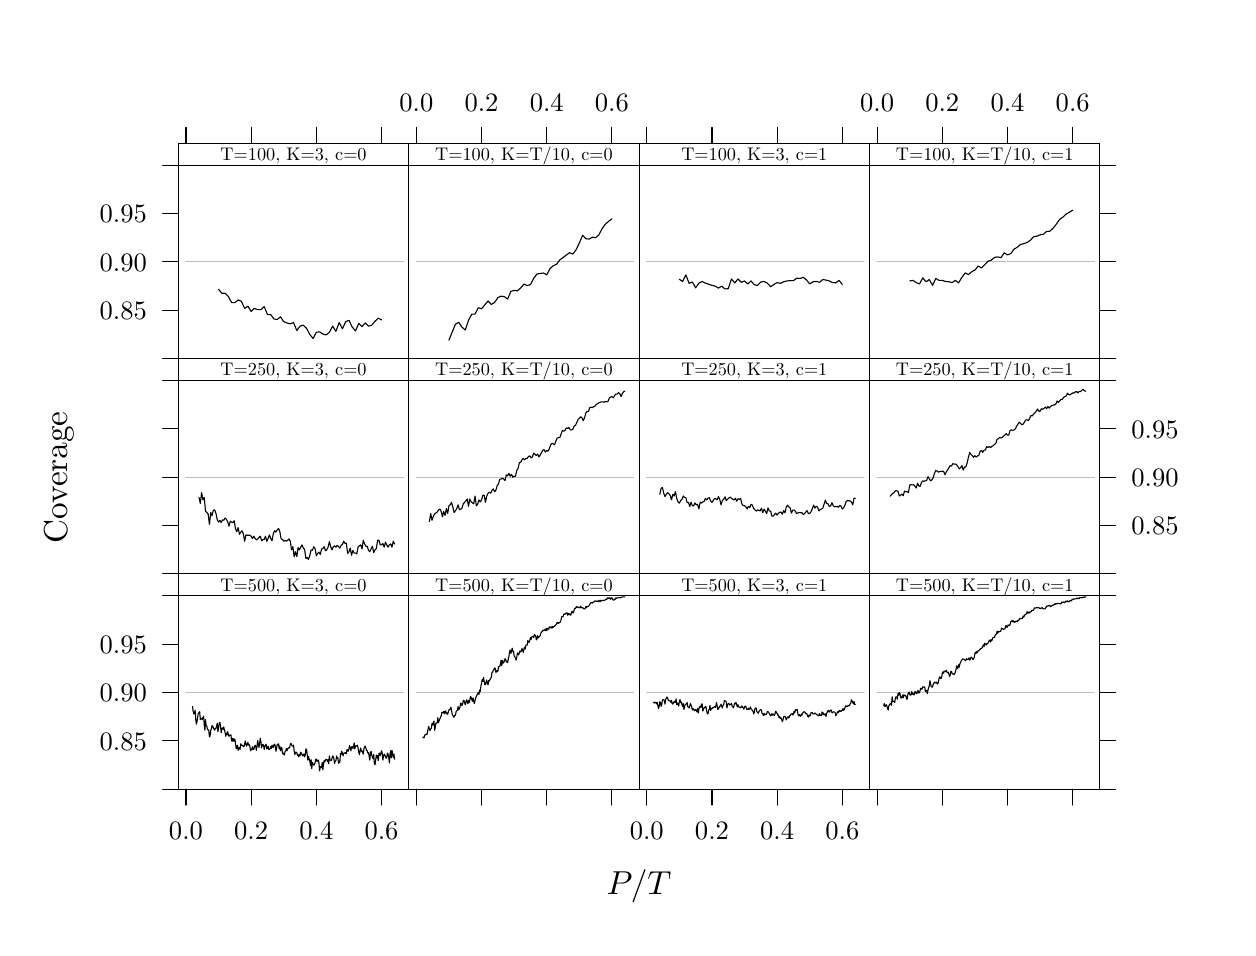
\begin{tikzpicture}[x=1pt,y=1pt]
\definecolor[named]{fillColor}{rgb}{1.00,1.00,1.00}
\path[use as bounding box,fill=fillColor,fill opacity=0.00] (0,0) rectangle (433.62,325.21);
\begin{scope}
\path[clip] (  0.00,  0.00) rectangle (433.62,325.21);

\path[] (  0.00,  0.00) rectangle (433.62,325.21);
\definecolor[named]{drawColor}{rgb}{0.00,0.00,0.00}

\node[text=drawColor,anchor=base,inner sep=0pt, outer sep=0pt, scale=  1.20] at (220.94, 12.05) {$P/T$};
\end{scope}
\begin{scope}
\path[clip] (  0.00,  0.00) rectangle (433.62,325.21);
\definecolor[named]{drawColor}{rgb}{0.00,0.00,0.00}

\node[text=drawColor,rotate= 90.00,anchor=base,inner sep=0pt, outer sep=0pt, scale=  1.20] at ( 14.29,162.76) {Coverage};
\end{scope}
\begin{scope}
\path[clip] (  0.00,  0.00) rectangle (433.62,325.21);
\definecolor[named]{drawColor}{rgb}{0.00,0.00,0.00}

\path[draw=drawColor,line width= 0.4pt,line join=round,line cap=round] ( 54.44, 50.02) -- ( 48.75, 50.02);

\path[draw=drawColor,line width= 0.4pt,line join=round,line cap=round] ( 54.44, 67.48) -- ( 48.75, 67.48);

\path[draw=drawColor,line width= 0.4pt,line join=round,line cap=round] ( 54.44, 84.95) -- ( 48.75, 84.95);

\path[draw=drawColor,line width= 0.4pt,line join=round,line cap=round] ( 54.44,102.42) -- ( 48.75,102.42);

\path[draw=drawColor,line width= 0.4pt,line join=round,line cap=round] ( 54.44,119.88) -- ( 48.75,119.88);

\node[text=drawColor,anchor=base east,inner sep=0pt, outer sep=0pt, scale=  0.96] at ( 43.06, 64.18) {0.85};

\node[text=drawColor,anchor=base east,inner sep=0pt, outer sep=0pt, scale=  0.96] at ( 43.06, 81.64) {0.90};

\node[text=drawColor,anchor=base east,inner sep=0pt, outer sep=0pt, scale=  0.96] at ( 43.06, 99.11) {0.95};
\end{scope}
\begin{scope}
\path[clip] (  0.00,  0.00) rectangle (433.62,325.21);
\definecolor[named]{drawColor}{rgb}{0.00,0.00,0.00}

\path[draw=drawColor,line width= 0.4pt,line join=round,line cap=round] ( 57.20, 50.02) -- ( 57.20, 44.32);

\path[draw=drawColor,line width= 0.4pt,line join=round,line cap=round] ( 80.76, 50.02) -- ( 80.76, 44.32);

\path[draw=drawColor,line width= 0.4pt,line join=round,line cap=round] (104.31, 50.02) -- (104.31, 44.32);

\path[draw=drawColor,line width= 0.4pt,line join=round,line cap=round] (127.87, 50.02) -- (127.87, 44.32);

\node[text=drawColor,anchor=base,inner sep=0pt, outer sep=0pt, scale=  0.96] at ( 57.20, 32.02) {0.0};

\node[text=drawColor,anchor=base,inner sep=0pt, outer sep=0pt, scale=  0.96] at ( 80.76, 32.02) {0.2};

\node[text=drawColor,anchor=base,inner sep=0pt, outer sep=0pt, scale=  0.96] at (104.31, 32.02) {0.4};

\node[text=drawColor,anchor=base,inner sep=0pt, outer sep=0pt, scale=  0.96] at (127.87, 32.02) {0.6};
\end{scope}
\begin{scope}
\path[clip] ( 54.44, 50.02) rectangle (137.69,119.88);
\definecolor[named]{drawColor}{rgb}{0.75,0.75,0.75}

\path[draw=drawColor,line width= 0.4pt,line join=round,line cap=round] ( 57.20, 84.95) --
	(135.72, 84.95);
\definecolor[named]{drawColor}{rgb}{0.00,0.00,0.00}

\path[draw=drawColor,line width= 0.4pt,line join=round,line cap=round] ( 59.56, 79.92) --
	( 59.79, 78.24) --
	( 60.03, 77.23) --
	( 60.26, 77.40) --
	( 60.50, 78.58) --
	( 60.73, 75.20) --
	( 60.97, 73.52) --
	( 61.20, 74.53) --
	( 61.44, 76.22) --
	( 61.68, 77.56) --
	( 61.91, 77.56) --
	( 62.15, 78.07) --
	( 62.38, 75.20) --
	( 62.62, 75.71) --
	( 62.85, 75.54) --
	( 63.09, 75.20) --
	( 63.32, 75.88) --
	( 63.56, 76.38) --
	( 63.80, 73.35) --
	( 64.03, 71.33) --
	( 64.27, 75.20) --
	( 64.50, 72.84) --
	( 64.74, 72.84) --
	( 64.97, 71.66) --
	( 65.21, 71.49) --
	( 65.44, 71.16) --
	( 65.68, 68.97) --
	( 65.92, 69.30) --
	( 66.15, 71.33) --
	( 66.39, 71.83) --
	( 66.62, 73.01) --
	( 66.86, 72.84) --
	( 67.09, 72.17) --
	( 67.33, 71.83) --
	( 67.56, 71.33) --
	( 67.80, 72.00) --
	( 68.04, 72.00) --
	( 68.27, 72.84) --
	( 68.51, 73.86) --
	( 68.74, 70.82) --
	( 68.98, 72.17) --
	( 69.21, 73.86) --
	( 69.45, 74.19) --
	( 69.69, 72.84) --
	( 69.92, 70.48) --
	( 70.16, 72.00) --
	( 70.39, 72.17) --
	( 70.63, 71.66) --
	( 70.86, 72.51) --
	( 71.10, 71.33) --
	( 71.33, 70.65) --
	( 71.57, 69.13) --
	( 71.81, 70.31) --
	( 72.04, 69.64) --
	( 72.28, 70.82) --
	( 72.51, 69.81) --
	( 72.75, 69.13) --
	( 72.98, 69.47) --
	( 73.22, 69.64) --
	( 73.45, 69.64) --
	( 73.69, 67.45) --
	( 73.93, 68.46) --
	( 74.16, 67.28) --
	( 74.40, 68.29) --
	( 74.63, 67.45) --
	( 74.87, 68.12) --
	( 75.10, 66.61) --
	( 75.34, 64.75) --
	( 75.57, 64.75) --
	( 75.81, 65.93) --
	( 76.05, 64.08) --
	( 76.28, 64.75) --
	( 76.52, 65.09) --
	( 76.75, 64.41) --
	( 76.99, 66.44) --
	( 77.22, 65.93) --
	( 77.46, 65.93) --
	( 77.69, 65.76) --
	( 77.93, 65.43) --
	( 78.17, 65.43) --
	( 78.40, 66.44) --
	( 78.64, 67.45) --
	( 78.87, 66.10) --
	( 79.11, 65.59) --
	( 79.34, 66.44) --
	( 79.58, 66.94) --
	( 79.81, 65.93) --
	( 80.05, 66.10) --
	( 80.29, 65.59) --
	( 80.52, 63.91) --
	( 80.76, 64.58) --
	( 80.99, 64.25) --
	( 81.23, 65.43) --
	( 81.46, 64.41) --
	( 81.70, 64.41) --
	( 81.93, 65.26) --
	( 82.17, 65.93) --
	( 82.41, 65.59) --
	( 82.64, 64.08) --
	( 82.88, 65.59) --
	( 83.11, 67.62) --
	( 83.35, 66.27) --
	( 83.58, 65.09) --
	( 83.82, 66.61) --
	( 84.05, 68.46) --
	( 84.29, 67.11) --
	( 84.53, 64.92) --
	( 84.76, 65.76) --
	( 85.00, 66.27) --
	( 85.23, 65.93) --
	( 85.47, 64.41) --
	( 85.70, 65.59) --
	( 85.94, 65.93) --
	( 86.17, 66.27) --
	( 86.41, 64.58) --
	( 86.65, 64.92) --
	( 86.88, 65.59) --
	( 87.12, 64.41) --
	( 87.35, 64.41) --
	( 87.59, 64.58) --
	( 87.82, 65.43) --
	( 88.06, 64.75) --
	( 88.29, 65.93) --
	( 88.53, 65.43) --
	( 88.77, 65.09) --
	( 89.00, 66.10) --
	( 89.24, 66.27) --
	( 89.47, 65.59) --
	( 89.71, 63.74) --
	( 89.94, 64.75) --
	( 90.18, 66.27) --
	( 90.41, 66.10) --
	( 90.65, 66.44) --
	( 90.89, 64.58) --
	( 91.12, 65.59) --
	( 91.36, 63.91) --
	( 91.59, 64.75) --
	( 91.83, 65.09) --
	( 92.06, 63.23) --
	( 92.30, 62.73) --
	( 92.53, 63.06) --
	( 92.77, 62.39) --
	( 93.01, 63.74) --
	( 93.24, 63.91) --
	( 93.48, 64.75) --
	( 93.71, 63.91) --
	( 93.95, 64.58) --
	( 94.18, 64.92) --
	( 94.42, 65.09) --
	( 94.66, 64.92) --
	( 94.89, 66.27) --
	( 95.13, 66.61) --
	( 95.36, 66.10) --
	( 95.60, 65.59) --
	( 95.83, 65.59) --
	( 96.07, 65.93) --
	( 96.30, 63.74) --
	( 96.54, 62.56) --
	( 96.78, 63.40) --
	( 97.01, 63.40) --
	( 97.25, 63.23) --
	( 97.48, 62.22) --
	( 97.72, 62.39) --
	( 97.95, 61.72) --
	( 98.19, 62.73) --
	( 98.42, 62.05) --
	( 98.66, 63.40) --
	( 98.90, 63.06) --
	( 99.13, 62.56) --
	( 99.37, 62.05) --
	( 99.60, 62.56) --
	( 99.84, 62.73) --
	(100.07, 61.72) --
	(100.31, 62.56) --
	(100.54, 64.58) --
	(100.78, 64.41) --
	(101.02, 62.39) --
	(101.25, 60.54) --
	(101.49, 61.88) --
	(101.72, 60.87) --
	(101.96, 60.20) --
	(102.19, 58.51) --
	(102.43, 60.70) --
	(102.66, 57.50) --
	(102.90, 59.69) --
	(103.14, 59.19) --
	(103.37, 58.68) --
	(103.61, 59.02) --
	(103.84, 59.52) --
	(104.08, 60.87) --
	(104.31, 60.87) --
	(104.55, 60.03) --
	(104.78, 60.54) --
	(105.02, 60.54) --
	(105.26, 59.52) --
	(105.49, 56.66) --
	(105.73, 58.18) --
	(105.96, 58.01) --
	(106.20, 57.84) --
	(106.43, 59.69) --
	(106.67, 57.00) --
	(106.90, 59.19) --
	(107.14, 60.37) --
	(107.38, 59.86) --
	(107.61, 60.70) --
	(107.85, 60.87) --
	(108.08, 60.70) --
	(108.32, 60.03) --
	(108.55, 60.70) --
	(108.79, 59.19) --
	(109.02, 62.05) --
	(109.26, 60.54) --
	(109.50, 60.54) --
	(109.73, 60.37) --
	(109.97, 61.21) --
	(110.20, 62.05) --
	(110.44, 61.72) --
	(110.67, 60.87) --
	(110.91, 59.36) --
	(111.14, 60.20) --
	(111.38, 60.37) --
	(111.62, 62.05) --
	(111.85, 61.21) --
	(112.09, 61.38) --
	(112.32, 59.36) --
	(112.56, 60.20) --
	(112.79, 59.69) --
	(113.03, 62.90) --
	(113.26, 62.56) --
	(113.50, 63.74) --
	(113.74, 63.06) --
	(113.97, 62.05) --
	(114.21, 63.06) --
	(114.44, 63.06) --
	(114.68, 63.23) --
	(114.91, 62.90) --
	(115.15, 62.90) --
	(115.38, 64.41) --
	(115.62, 63.91) --
	(115.86, 63.74) --
	(116.09, 64.75) --
	(116.33, 65.76) --
	(116.56, 64.75) --
	(116.80, 63.91) --
	(117.03, 65.26) --
	(117.27, 65.43) --
	(117.51, 64.75) --
	(117.74, 65.26) --
	(117.98, 66.77) --
	(118.21, 64.58) --
	(118.45, 65.59) --
	(118.68, 65.76) --
	(118.92, 65.59) --
	(119.15, 65.93) --
	(119.39, 64.92) --
	(119.63, 63.40) --
	(119.86, 62.56) --
	(120.10, 63.91) --
	(120.33, 64.92) --
	(120.57, 63.74) --
	(120.80, 63.91) --
	(121.04, 63.23) --
	(121.27, 62.73) --
	(121.51, 64.75) --
	(121.75, 65.26) --
	(121.98, 65.59) --
	(122.22, 64.92) --
	(122.45, 64.08) --
	(122.69, 63.91) --
	(122.92, 63.06) --
	(123.16, 63.23) --
	(123.39, 61.88) --
	(123.63, 60.54) --
	(123.87, 63.23) --
	(124.10, 63.74) --
	(124.34, 62.22) --
	(124.57, 61.72) --
	(124.81, 61.04) --
	(125.04, 62.56) --
	(125.28, 59.19) --
	(125.51, 58.85) --
	(125.75, 60.54) --
	(125.99, 62.39) --
	(126.22, 61.38) --
	(126.46, 62.22) --
	(126.69, 60.37) --
	(126.93, 62.90) --
	(127.16, 63.06) --
	(127.40, 62.22) --
	(127.63, 62.90) --
	(127.87, 63.91) --
	(128.11, 63.06) --
	(128.34, 60.54) --
	(128.58, 61.88) --
	(128.81, 62.73) --
	(129.05, 62.39) --
	(129.28, 61.88) --
	(129.52, 61.21) --
	(129.75, 61.38) --
	(129.99, 63.06) --
	(130.23, 62.73) --
	(130.46, 61.55) --
	(130.70, 59.52) --
	(130.93, 62.73) --
	(131.17, 63.91) --
	(131.40, 61.38) --
	(131.64, 64.08) --
	(131.87, 62.90) --
	(132.11, 61.55) --
	(132.35, 62.73) --
	(132.58, 60.87);
\end{scope}
\begin{scope}
\path[clip] (  0.00,  0.00) rectangle (433.62,325.21);
\definecolor[named]{drawColor}{rgb}{0.00,0.00,0.00}

\path[draw=drawColor,line width= 0.4pt,line join=round,line cap=round] ( 54.44, 50.02) rectangle (137.69,119.88);
\end{scope}
\begin{scope}
\path[clip] ( 54.44,119.88) rectangle (137.69,127.83);

\path[] ( 54.44,119.88) rectangle (137.69,127.83);
\definecolor[named]{drawColor}{rgb}{0.00,0.00,0.00}

\node[text=drawColor,anchor=base west,inner sep=0pt, outer sep=0pt, scale=  0.66] at ( 69.67,121.58) {T=500, K=3, c=0};
\end{scope}
\begin{scope}
\path[clip] (  0.00,  0.00) rectangle (433.62,325.21);
\definecolor[named]{drawColor}{rgb}{0.00,0.00,0.00}

\path[draw=drawColor,line width= 0.4pt,line join=round,line cap=round] ( 54.44,119.88) rectangle (137.69,127.83);
\end{scope}
\begin{scope}
\path[clip] (  0.00,  0.00) rectangle (433.62,325.21);
\definecolor[named]{drawColor}{rgb}{0.00,0.00,0.00}

\path[draw=drawColor,line width= 0.4pt,line join=round,line cap=round] (140.45, 50.02) -- (140.45, 44.32);

\path[draw=drawColor,line width= 0.4pt,line join=round,line cap=round] (164.01, 50.02) -- (164.01, 44.32);

\path[draw=drawColor,line width= 0.4pt,line join=round,line cap=round] (187.56, 50.02) -- (187.56, 44.32);

\path[draw=drawColor,line width= 0.4pt,line join=round,line cap=round] (211.12, 50.02) -- (211.12, 44.32);
\end{scope}
\begin{scope}
\path[clip] (137.69, 50.02) rectangle (220.94,119.88);
\definecolor[named]{drawColor}{rgb}{0.75,0.75,0.75}

\path[draw=drawColor,line width= 0.4pt,line join=round,line cap=round] (140.45, 84.95) --
	(218.97, 84.95);
\definecolor[named]{drawColor}{rgb}{0.00,0.00,0.00}

\path[draw=drawColor,line width= 0.4pt,line join=round,line cap=round] (142.80, 68.53) --
	(143.04, 68.88) --
	(143.28, 68.70) --
	(143.51, 69.58) --
	(143.75, 69.75) --
	(143.98, 69.93) --
	(144.22, 69.75) --
	(144.45, 70.45) --
	(144.69, 71.85) --
	(144.92, 72.72) --
	(145.16, 71.85) --
	(145.40, 71.15) --
	(145.63, 71.85) --
	(145.87, 72.02) --
	(146.10, 73.77) --
	(146.34, 73.25) --
	(146.57, 74.12) --
	(146.81, 74.64) --
	(147.05, 71.32) --
	(147.28, 72.37) --
	(147.52, 73.94) --
	(147.75, 73.94) --
	(147.99, 73.94) --
	(148.22, 75.87) --
	(148.46, 74.12) --
	(148.69, 74.82) --
	(148.93, 75.34) --
	(149.17, 76.04) --
	(149.40, 76.39) --
	(149.64, 77.79) --
	(149.87, 77.79) --
	(150.11, 77.61) --
	(150.34, 78.14) --
	(150.58, 77.26) --
	(150.81, 78.14) --
	(151.05, 78.31) --
	(151.29, 77.26) --
	(151.52, 77.61) --
	(151.76, 77.09) --
	(151.99, 77.96) --
	(152.23, 78.66) --
	(152.46, 78.84) --
	(152.70, 79.01) --
	(152.93, 79.71) --
	(153.17, 78.49) --
	(153.41, 77.09) --
	(153.64, 76.74) --
	(153.88, 76.04) --
	(154.11, 76.22) --
	(154.35, 76.74) --
	(154.58, 76.74) --
	(154.82, 78.14) --
	(155.05, 78.31) --
	(155.29, 78.66) --
	(155.53, 79.88) --
	(155.76, 78.66) --
	(156.00, 79.18) --
	(156.23, 79.71) --
	(156.47, 81.11) --
	(156.70, 80.93) --
	(156.94, 80.23) --
	(157.17, 80.76) --
	(157.41, 82.15) --
	(157.65, 82.15) --
	(157.88, 81.28) --
	(158.12, 80.58) --
	(158.35, 81.46) --
	(158.59, 82.33) --
	(158.82, 81.63) --
	(159.06, 80.93) --
	(159.29, 82.15) --
	(159.53, 81.28) --
	(159.77, 82.15) --
	(160.00, 83.55) --
	(160.24, 83.20) --
	(160.47, 82.50) --
	(160.71, 81.80) --
	(160.94, 83.03) --
	(161.18, 81.80) --
	(161.41, 80.93) --
	(161.65, 81.98) --
	(161.89, 83.03) --
	(162.12, 83.55) --
	(162.36, 84.08) --
	(162.59, 84.42) --
	(162.83, 84.95) --
	(163.06, 84.25) --
	(163.30, 85.82) --
	(163.53, 85.30) --
	(163.77, 87.22) --
	(164.01, 88.44) --
	(164.24, 89.66) --
	(164.48, 88.97) --
	(164.71, 90.36) --
	(164.95, 89.14) --
	(165.18, 87.74) --
	(165.42, 87.92) --
	(165.65, 88.79) --
	(165.89, 89.49) --
	(166.13, 88.09) --
	(166.36, 87.74) --
	(166.60, 89.32) --
	(166.83, 89.14) --
	(167.07, 89.66) --
	(167.30, 90.19) --
	(167.54, 90.36) --
	(167.77, 92.28) --
	(168.01, 92.28) --
	(168.25, 92.98) --
	(168.48, 93.33) --
	(168.72, 93.86) --
	(168.95, 93.68) --
	(169.19, 92.28) --
	(169.42, 92.46) --
	(169.66, 92.98) --
	(169.90, 92.63) --
	(170.13, 94.21) --
	(170.37, 94.38) --
	(170.60, 94.38) --
	(170.84, 95.43) --
	(171.07, 96.65) --
	(171.31, 94.73) --
	(171.54, 96.48) --
	(171.78, 95.60) --
	(172.02, 95.78) --
	(172.25, 96.48) --
	(172.49, 97.18) --
	(172.72, 97.00) --
	(172.96, 95.95) --
	(173.19, 96.30) --
	(173.43, 95.78) --
	(173.66, 97.00) --
	(173.90, 98.05) --
	(174.14, 99.80) --
	(174.37,100.32) --
	(174.61, 99.10) --
	(174.84, 99.97) --
	(175.08,101.02) --
	(175.31, 99.80) --
	(175.55, 99.97) --
	(175.78, 98.22) --
	(176.02, 97.87) --
	(176.26, 97.35) --
	(176.49, 96.65) --
	(176.73, 97.70) --
	(176.96, 99.27) --
	(177.20, 98.92) --
	(177.43, 98.57) --
	(177.67, 99.45) --
	(177.90, 99.97) --
	(178.14, 99.62) --
	(178.38, 99.97) --
	(178.61,100.84) --
	(178.85,100.32) --
	(179.08, 99.45) --
	(179.32,100.67) --
	(179.55,101.37) --
	(179.79,100.67) --
	(180.02,102.07) --
	(180.26,102.07) --
	(180.50,102.07) --
	(180.73,103.81) --
	(180.97,103.11) --
	(181.20,103.11) --
	(181.44,103.81) --
	(181.67,104.86) --
	(181.91,104.16) --
	(182.14,105.04) --
	(182.38,105.21) --
	(182.62,105.21) --
	(182.85,104.86) --
	(183.09,105.91) --
	(183.32,105.73) --
	(183.56,105.38) --
	(183.79,103.99) --
	(184.03,104.34) --
	(184.26,105.56) --
	(184.50,104.69) --
	(184.74,105.04) --
	(184.97,105.21) --
	(185.21,105.56) --
	(185.44,106.43) --
	(185.68,106.78) --
	(185.91,106.96) --
	(186.15,107.48) --
	(186.38,107.31) --
	(186.62,107.48) --
	(186.86,107.66) --
	(187.09,107.31) --
	(187.33,108.18) --
	(187.56,107.31) --
	(187.80,108.00) --
	(188.03,108.18) --
	(188.27,107.83) --
	(188.50,108.70) --
	(188.74,108.35) --
	(188.98,108.70) --
	(189.21,108.70) --
	(189.45,108.18) --
	(189.68,108.88) --
	(189.92,108.53) --
	(190.15,108.88) --
	(190.39,108.88) --
	(190.62,109.23) --
	(190.86,109.40) --
	(191.10,109.75) --
	(191.33,110.28) --
	(191.57,110.10) --
	(191.80,109.93) --
	(192.04,110.28) --
	(192.27,110.28) --
	(192.51,110.45) --
	(192.74,111.32) --
	(192.98,112.37) --
	(193.22,112.37) --
	(193.45,112.37) --
	(193.69,113.24) --
	(193.92,113.42) --
	(194.16,113.24) --
	(194.39,113.59) --
	(194.63,113.59) --
	(194.87,113.77) --
	(195.10,112.90) --
	(195.34,113.59) --
	(195.57,113.07) --
	(195.81,113.42) --
	(196.04,113.07) --
	(196.28,112.90) --
	(196.51,114.12) --
	(196.75,114.29) --
	(196.99,113.77) --
	(197.22,113.77) --
	(197.46,114.82) --
	(197.69,115.34) --
	(197.93,115.34) --
	(198.16,115.86) --
	(198.40,116.04) --
	(198.63,115.69) --
	(198.87,115.86) --
	(199.11,115.69) --
	(199.34,115.69) --
	(199.58,115.52) --
	(199.81,116.21) --
	(200.05,115.69) --
	(200.28,115.69) --
	(200.52,115.52) --
	(200.75,115.52) --
	(200.99,115.17) --
	(201.23,115.17) --
	(201.46,115.34) --
	(201.70,116.04) --
	(201.93,115.69) --
	(202.17,116.04) --
	(202.40,116.04) --
	(202.64,116.21) --
	(202.87,116.39) --
	(203.11,116.91) --
	(203.35,117.26) --
	(203.58,117.44) --
	(203.82,117.44) --
	(204.05,117.26) --
	(204.29,117.61) --
	(204.52,117.61) --
	(204.76,117.96) --
	(204.99,117.96) --
	(205.23,118.14) --
	(205.47,117.96) --
	(205.70,117.96) --
	(205.94,117.96) --
	(206.17,117.79) --
	(206.41,118.31) --
	(206.64,117.96) --
	(206.88,117.79) --
	(207.11,118.31) --
	(207.35,118.14) --
	(207.59,118.14) --
	(207.82,118.31) --
	(208.06,118.14) --
	(208.29,118.31) --
	(208.53,118.31) --
	(208.76,118.48) --
	(209.00,118.66) --
	(209.23,118.66) --
	(209.47,119.18) --
	(209.71,118.83) --
	(209.94,119.18) --
	(210.18,119.01) --
	(210.41,119.18) --
	(210.65,118.66) --
	(210.88,119.18) --
	(211.12,119.18) --
	(211.35,118.66) --
	(211.59,118.48) --
	(211.83,118.31) --
	(212.06,118.66) --
	(212.30,118.66) --
	(212.53,119.18) --
	(212.77,119.01) --
	(213.00,119.18) --
	(213.24,119.18) --
	(213.47,119.18) --
	(213.71,119.36) --
	(213.95,119.36) --
	(214.18,119.18) --
	(214.42,119.36) --
	(214.65,119.36) --
	(214.89,119.53) --
	(215.12,119.53) --
	(215.36,119.53) --
	(215.59,119.53) --
	(215.83,119.53);
\end{scope}
\begin{scope}
\path[clip] (  0.00,  0.00) rectangle (433.62,325.21);
\definecolor[named]{drawColor}{rgb}{0.00,0.00,0.00}

\path[draw=drawColor,line width= 0.4pt,line join=round,line cap=round] (137.69, 50.02) rectangle (220.94,119.88);
\end{scope}
\begin{scope}
\path[clip] (137.69,119.88) rectangle (220.94,127.83);

\path[] (137.69,119.88) rectangle (220.94,127.83);
\definecolor[named]{drawColor}{rgb}{0.00,0.00,0.00}

\node[text=drawColor,anchor=base west,inner sep=0pt, outer sep=0pt, scale=  0.66] at (147.24,121.58) {T=500, K=T/10, c=0};
\end{scope}
\begin{scope}
\path[clip] (  0.00,  0.00) rectangle (433.62,325.21);
\definecolor[named]{drawColor}{rgb}{0.00,0.00,0.00}

\path[draw=drawColor,line width= 0.4pt,line join=round,line cap=round] (137.69,119.88) rectangle (220.94,127.83);
\end{scope}
\begin{scope}
\path[clip] (  0.00,  0.00) rectangle (433.62,325.21);
\definecolor[named]{drawColor}{rgb}{0.00,0.00,0.00}

\path[draw=drawColor,line width= 0.4pt,line join=round,line cap=round] (223.70, 50.02) -- (223.70, 44.32);

\path[draw=drawColor,line width= 0.4pt,line join=round,line cap=round] (247.26, 50.02) -- (247.26, 44.32);

\path[draw=drawColor,line width= 0.4pt,line join=round,line cap=round] (270.81, 50.02) -- (270.81, 44.32);

\path[draw=drawColor,line width= 0.4pt,line join=round,line cap=round] (294.37, 50.02) -- (294.37, 44.32);

\node[text=drawColor,anchor=base,inner sep=0pt, outer sep=0pt, scale=  0.96] at (223.70, 32.02) {0.0};

\node[text=drawColor,anchor=base,inner sep=0pt, outer sep=0pt, scale=  0.96] at (247.26, 32.02) {0.2};

\node[text=drawColor,anchor=base,inner sep=0pt, outer sep=0pt, scale=  0.96] at (270.81, 32.02) {0.4};

\node[text=drawColor,anchor=base,inner sep=0pt, outer sep=0pt, scale=  0.96] at (294.37, 32.02) {0.6};
\end{scope}
\begin{scope}
\path[clip] (220.94, 50.02) rectangle (304.19,119.88);
\definecolor[named]{drawColor}{rgb}{0.75,0.75,0.75}

\path[draw=drawColor,line width= 0.4pt,line join=round,line cap=round] (223.70, 84.95) --
	(302.22, 84.95);
\definecolor[named]{drawColor}{rgb}{0.00,0.00,0.00}

\path[draw=drawColor,line width= 0.4pt,line join=round,line cap=round] (226.05, 81.26) --
	(226.29, 81.46) --
	(226.53, 81.16) --
	(226.76, 81.36) --
	(227.00, 81.46) --
	(227.23, 80.86) --
	(227.47, 81.36) --
	(227.70, 80.36) --
	(227.94, 79.16) --
	(228.17, 79.96) --
	(228.41, 81.66) --
	(228.65, 81.26) --
	(228.88, 79.96) --
	(229.12, 80.56) --
	(229.35, 82.25) --
	(229.59, 82.35) --
	(229.82, 82.35) --
	(230.06, 82.05) --
	(230.29, 80.76) --
	(230.53, 82.45) --
	(230.77, 82.95) --
	(231.00, 83.35) --
	(231.24, 82.85) --
	(231.47, 82.25) --
	(231.71, 82.05) --
	(231.94, 81.95) --
	(232.18, 81.85) --
	(232.41, 81.46) --
	(232.65, 82.15) --
	(232.89, 80.96) --
	(233.12, 80.76) --
	(233.36, 81.16) --
	(233.59, 81.75) --
	(233.83, 81.46) --
	(234.06, 81.36) --
	(234.30, 82.65) --
	(234.53, 80.56) --
	(234.77, 81.16) --
	(235.01, 80.86) --
	(235.24, 80.06) --
	(235.48, 81.66) --
	(235.71, 82.45) --
	(235.95, 81.36) --
	(236.18, 81.56) --
	(236.42, 80.56) --
	(236.65, 79.96) --
	(236.89, 80.96) --
	(237.13, 78.86) --
	(237.36, 79.76) --
	(237.60, 80.76) --
	(237.83, 80.76) --
	(238.07, 80.76) --
	(238.30, 81.36) --
	(238.54, 79.76) --
	(238.77, 79.76) --
	(239.01, 79.36) --
	(239.25, 80.16) --
	(239.48, 80.96) --
	(239.72, 80.36) --
	(239.95, 79.76) --
	(240.19, 78.66) --
	(240.42, 79.16) --
	(240.66, 78.96) --
	(240.89, 78.36) --
	(241.13, 78.46) --
	(241.37, 78.86) --
	(241.60, 78.46) --
	(241.84, 77.96) --
	(242.07, 79.26) --
	(242.31, 77.56) --
	(242.54, 78.96) --
	(242.78, 79.76) --
	(243.01, 79.96) --
	(243.25, 79.56) --
	(243.49, 80.76) --
	(243.72, 80.86) --
	(243.96, 78.26) --
	(244.19, 78.96) --
	(244.43, 79.46) --
	(244.66, 79.46) --
	(244.90, 79.96) --
	(245.13, 79.76) --
	(245.37, 78.16) --
	(245.61, 77.26) --
	(245.84, 77.26) --
	(246.08, 78.56) --
	(246.31, 78.96) --
	(246.55, 80.26) --
	(246.78, 78.46) --
	(247.02, 79.16) --
	(247.26, 79.06) --
	(247.49, 79.46) --
	(247.73, 79.46) --
	(247.96, 79.76) --
	(248.20, 79.86) --
	(248.43, 79.56) --
	(248.67, 80.06) --
	(248.90, 81.36) --
	(249.14, 80.16) --
	(249.38, 78.86) --
	(249.61, 79.06) --
	(249.85, 79.46) --
	(250.08, 80.06) --
	(250.32, 80.06) --
	(250.55, 80.76) --
	(250.79, 79.96) --
	(251.02, 79.36) --
	(251.26, 80.36) --
	(251.50, 80.56) --
	(251.73, 82.05) --
	(251.97, 81.95) --
	(252.20, 81.95) --
	(252.44, 81.46) --
	(252.67, 79.36) --
	(252.91, 80.56) --
	(253.14, 80.96) --
	(253.38, 81.06) --
	(253.62, 80.46) --
	(253.85, 80.66) --
	(254.09, 80.56) --
	(254.32, 81.06) --
	(254.56, 80.06) --
	(254.79, 79.76) --
	(255.03, 79.46) --
	(255.26, 80.36) --
	(255.50, 81.16) --
	(255.74, 80.86) --
	(255.97, 81.36) --
	(256.21, 80.46) --
	(256.44, 79.76) --
	(256.68, 80.56) --
	(256.91, 79.76) --
	(257.15, 79.66) --
	(257.38, 79.66) --
	(257.62, 79.46) --
	(257.86, 79.76) --
	(258.09, 80.16) --
	(258.33, 79.56) --
	(258.56, 79.46) --
	(258.80, 78.96) --
	(259.03, 79.86) --
	(259.27, 79.96) --
	(259.50, 80.06) --
	(259.74, 79.06) --
	(259.98, 78.86) --
	(260.21, 78.96) --
	(260.45, 79.26) --
	(260.68, 78.86) --
	(260.92, 79.16) --
	(261.15, 79.76) --
	(261.39, 78.96) --
	(261.62, 78.96) --
	(261.86, 78.46) --
	(262.10, 78.26) --
	(262.33, 77.26) --
	(262.57, 77.76) --
	(262.80, 79.26) --
	(263.04, 79.46) --
	(263.27, 79.26) --
	(263.51, 77.96) --
	(263.74, 77.76) --
	(263.98, 77.46) --
	(264.22, 78.06) --
	(264.45, 78.36) --
	(264.69, 78.66) --
	(264.92, 78.76) --
	(265.16, 78.56) --
	(265.39, 77.26) --
	(265.63, 77.26) --
	(265.86, 76.66) --
	(266.10, 77.46) --
	(266.34, 76.86) --
	(266.57, 77.16) --
	(266.81, 77.06) --
	(267.04, 77.26) --
	(267.28, 78.06) --
	(267.51, 77.96) --
	(267.75, 77.96) --
	(267.98, 77.26) --
	(268.22, 76.96) --
	(268.46, 76.56) --
	(268.69, 76.86) --
	(268.93, 77.36) --
	(269.16, 76.76) --
	(269.40, 77.06) --
	(269.63, 77.16) --
	(269.87, 76.66) --
	(270.11, 77.56) --
	(270.34, 78.26) --
	(270.58, 77.66) --
	(270.81, 77.46) --
	(271.05, 76.76) --
	(271.28, 76.86) --
	(271.52, 75.77) --
	(271.75, 76.27) --
	(271.99, 75.67) --
	(272.23, 75.77) --
	(272.46, 75.17) --
	(272.70, 74.47) --
	(272.93, 75.07) --
	(273.17, 76.27) --
	(273.40, 76.17) --
	(273.64, 76.46) --
	(273.87, 75.97) --
	(274.11, 75.07) --
	(274.35, 75.67) --
	(274.58, 76.17) --
	(274.82, 76.17) --
	(275.05, 75.77) --
	(275.29, 76.56) --
	(275.52, 76.56) --
	(275.76, 77.06) --
	(275.99, 77.16) --
	(276.23, 77.36) --
	(276.47, 76.86) --
	(276.70, 77.16) --
	(276.94, 78.26) --
	(277.17, 77.66) --
	(277.41, 78.46) --
	(277.64, 78.86) --
	(277.88, 78.56) --
	(278.11, 78.76) --
	(278.35, 77.06) --
	(278.59, 76.56) --
	(278.82, 76.96) --
	(279.06, 76.56) --
	(279.29, 76.37) --
	(279.53, 77.16) --
	(279.76, 76.76) --
	(280.00, 77.46) --
	(280.23, 77.76) --
	(280.47, 77.96) --
	(280.71, 78.06) --
	(280.94, 77.66) --
	(281.18, 77.26) --
	(281.41, 77.46) --
	(281.65, 76.96) --
	(281.88, 76.37) --
	(282.12, 76.07) --
	(282.35, 76.86) --
	(282.59, 76.46) --
	(282.83, 76.76) --
	(283.06, 77.66) --
	(283.30, 77.76) --
	(283.53, 77.66) --
	(283.77, 77.16) --
	(284.00, 77.26) --
	(284.24, 77.26) --
	(284.47, 77.56) --
	(284.71, 77.36) --
	(284.95, 77.16) --
	(285.18, 76.96) --
	(285.42, 76.76) --
	(285.65, 76.66) --
	(285.89, 76.56) --
	(286.12, 77.36) --
	(286.36, 76.66) --
	(286.59, 76.86) --
	(286.83, 76.66) --
	(287.07, 77.96) --
	(287.30, 77.16) --
	(287.54, 77.56) --
	(287.77, 76.86) --
	(288.01, 77.06) --
	(288.24, 77.26) --
	(288.48, 76.27) --
	(288.71, 77.46) --
	(288.95, 77.96) --
	(289.19, 78.46) --
	(289.42, 78.46) --
	(289.66, 77.86) --
	(289.89, 78.26) --
	(290.13, 78.56) --
	(290.36, 78.66) --
	(290.60, 77.66) --
	(290.83, 77.66) --
	(291.07, 77.96) --
	(291.31, 77.96) --
	(291.54, 77.96) --
	(291.78, 77.66) --
	(292.01, 76.56) --
	(292.25, 77.06) --
	(292.48, 77.56) --
	(292.72, 78.06) --
	(292.96, 77.76) --
	(293.19, 78.46) --
	(293.43, 78.06) --
	(293.66, 78.36) --
	(293.90, 78.16) --
	(294.13, 78.46) --
	(294.37, 78.56) --
	(294.60, 79.16) --
	(294.84, 78.56) --
	(295.08, 78.76) --
	(295.31, 79.46) --
	(295.55, 80.16) --
	(295.78, 80.06) --
	(296.02, 79.86) --
	(296.25, 79.96) --
	(296.49, 80.36) --
	(296.72, 80.16) --
	(296.96, 80.26) --
	(297.20, 80.96) --
	(297.43, 81.16) --
	(297.67, 82.35) --
	(297.90, 81.95) --
	(298.14, 81.36) --
	(298.37, 80.86) --
	(298.61, 81.75) --
	(298.84, 80.56) --
	(299.08, 80.76);
\end{scope}
\begin{scope}
\path[clip] (  0.00,  0.00) rectangle (433.62,325.21);
\definecolor[named]{drawColor}{rgb}{0.00,0.00,0.00}

\path[draw=drawColor,line width= 0.4pt,line join=round,line cap=round] (220.94, 50.02) rectangle (304.19,119.88);
\end{scope}
\begin{scope}
\path[clip] (220.94,119.88) rectangle (304.19,127.83);

\path[] (220.94,119.88) rectangle (304.19,127.83);
\definecolor[named]{drawColor}{rgb}{0.00,0.00,0.00}

\node[text=drawColor,anchor=base west,inner sep=0pt, outer sep=0pt, scale=  0.66] at (236.17,121.58) {T=500, K=3, c=1};
\end{scope}
\begin{scope}
\path[clip] (  0.00,  0.00) rectangle (433.62,325.21);
\definecolor[named]{drawColor}{rgb}{0.00,0.00,0.00}

\path[draw=drawColor,line width= 0.4pt,line join=round,line cap=round] (220.94,119.88) rectangle (304.19,127.83);
\end{scope}
\begin{scope}
\path[clip] (  0.00,  0.00) rectangle (433.62,325.21);
\definecolor[named]{drawColor}{rgb}{0.00,0.00,0.00}

\path[draw=drawColor,line width= 0.4pt,line join=round,line cap=round] (306.95, 50.02) -- (306.95, 44.32);

\path[draw=drawColor,line width= 0.4pt,line join=round,line cap=round] (330.50, 50.02) -- (330.50, 44.32);

\path[draw=drawColor,line width= 0.4pt,line join=round,line cap=round] (354.06, 50.02) -- (354.06, 44.32);

\path[draw=drawColor,line width= 0.4pt,line join=round,line cap=round] (377.62, 50.02) -- (377.62, 44.32);

\path[draw=drawColor,line width= 0.4pt,line join=round,line cap=round] (387.44, 50.02) -- (393.13, 50.02);

\path[draw=drawColor,line width= 0.4pt,line join=round,line cap=round] (387.44, 67.48) -- (393.13, 67.48);

\path[draw=drawColor,line width= 0.4pt,line join=round,line cap=round] (387.44, 84.95) -- (393.13, 84.95);

\path[draw=drawColor,line width= 0.4pt,line join=round,line cap=round] (387.44,102.42) -- (393.13,102.42);

\path[draw=drawColor,line width= 0.4pt,line join=round,line cap=round] (387.44,119.88) -- (393.13,119.88);
\end{scope}
\begin{scope}
\path[clip] (304.19, 50.02) rectangle (387.44,119.88);
\definecolor[named]{drawColor}{rgb}{0.75,0.75,0.75}

\path[draw=drawColor,line width= 0.4pt,line join=round,line cap=round] (306.95, 84.95) --
	(385.47, 84.95);
\definecolor[named]{drawColor}{rgb}{0.00,0.00,0.00}

\path[draw=drawColor,line width= 0.4pt,line join=round,line cap=round] (309.30, 80.26) --
	(309.54, 80.96) --
	(309.77, 79.86) --
	(310.01, 80.16) --
	(310.25, 80.56) --
	(310.48, 80.16) --
	(310.72, 79.16) --
	(310.95, 78.66) --
	(311.19, 80.16) --
	(311.42, 80.66) --
	(311.66, 80.76) --
	(311.89, 81.06) --
	(312.13, 80.36) --
	(312.37, 83.45) --
	(312.60, 81.75) --
	(312.84, 81.66) --
	(313.07, 81.75) --
	(313.31, 81.36) --
	(313.54, 82.95) --
	(313.78, 83.45) --
	(314.01, 83.25) --
	(314.25, 82.55) --
	(314.49, 84.65) --
	(314.72, 84.05) --
	(314.96, 84.95) --
	(315.19, 84.65) --
	(315.43, 83.25) --
	(315.66, 82.95) --
	(315.90, 83.25) --
	(316.13, 84.05) --
	(316.37, 83.05) --
	(316.61, 84.15) --
	(316.84, 83.85) --
	(317.08, 83.95) --
	(317.31, 83.75) --
	(317.55, 82.95) --
	(317.78, 82.45) --
	(318.02, 84.05) --
	(318.25, 84.85) --
	(318.49, 85.15) --
	(318.73, 84.25) --
	(318.96, 84.05) --
	(319.20, 84.05) --
	(319.43, 85.35) --
	(319.67, 84.35) --
	(319.90, 84.75) --
	(320.14, 84.15) --
	(320.37, 84.15) --
	(320.61, 85.35) --
	(320.85, 85.15) --
	(321.08, 84.65) --
	(321.32, 84.55) --
	(321.55, 85.55) --
	(321.79, 85.65) --
	(322.02, 84.75) --
	(322.26, 85.05) --
	(322.50, 85.75) --
	(322.73, 86.55) --
	(322.97, 86.15) --
	(323.20, 86.35) --
	(323.44, 87.04) --
	(323.67, 86.85) --
	(323.91, 87.04) --
	(324.14, 86.85) --
	(324.38, 85.35) --
	(324.62, 85.85) --
	(324.85, 85.55) --
	(325.09, 84.55) --
	(325.32, 85.85) --
	(325.56, 86.75) --
	(325.79, 87.44) --
	(326.03, 89.24) --
	(326.26, 88.14) --
	(326.50, 87.04) --
	(326.74, 86.94) --
	(326.97, 87.04) --
	(327.21, 87.84) --
	(327.44, 88.34) --
	(327.68, 88.74) --
	(327.91, 88.44) --
	(328.15, 88.54) --
	(328.38, 88.74) --
	(328.62, 88.14) --
	(328.86, 88.04) --
	(329.09, 88.74) --
	(329.33, 90.04) --
	(329.56, 90.64) --
	(329.80, 90.34) --
	(330.03, 89.94) --
	(330.27, 90.64) --
	(330.50, 91.94) --
	(330.74, 92.43) --
	(330.98, 91.94) --
	(331.21, 92.73) --
	(331.45, 92.53) --
	(331.68, 92.63) --
	(331.92, 93.03) --
	(332.15, 92.33) --
	(332.39, 92.14) --
	(332.62, 92.33) --
	(332.86, 91.74) --
	(333.10, 90.74) --
	(333.33, 91.14) --
	(333.57, 92.63) --
	(333.80, 92.63) --
	(334.04, 91.84) --
	(334.27, 91.64) --
	(334.51, 91.74) --
	(334.74, 91.44) --
	(334.98, 91.74) --
	(335.22, 92.53) --
	(335.45, 93.23) --
	(335.69, 94.63) --
	(335.92, 93.73) --
	(336.16, 93.73) --
	(336.39, 95.03) --
	(336.63, 94.13) --
	(336.86, 95.43) --
	(337.10, 95.73) --
	(337.34, 96.43) --
	(337.57, 96.73) --
	(337.81, 97.13) --
	(338.04, 97.03) --
	(338.28, 97.03) --
	(338.51, 96.83) --
	(338.75, 96.63) --
	(338.98, 96.43) --
	(339.22, 97.23) --
	(339.46, 96.93) --
	(339.69, 96.93) --
	(339.93, 96.93) --
	(340.16, 97.52) --
	(340.40, 96.63) --
	(340.63, 97.13) --
	(340.87, 97.72) --
	(341.10, 97.72) --
	(341.34, 97.23) --
	(341.58, 96.83) --
	(341.81, 97.33) --
	(342.05, 97.62) --
	(342.28, 99.12) --
	(342.52, 99.52) --
	(342.75, 99.12) --
	(342.99, 99.82) --
	(343.22, 99.52) --
	(343.46,100.12) --
	(343.70,100.12) --
	(343.93,100.32) --
	(344.17,100.62) --
	(344.40,100.92) --
	(344.64,100.92) --
	(344.87,101.12) --
	(345.11,101.72) --
	(345.35,102.22) --
	(345.58,101.52) --
	(345.82,102.81) --
	(346.05,102.42) --
	(346.29,102.12) --
	(346.52,102.62) --
	(346.76,102.52) --
	(346.99,102.81) --
	(347.23,103.31) --
	(347.47,103.91) --
	(347.70,103.81) --
	(347.94,103.21) --
	(348.17,104.11) --
	(348.41,103.71) --
	(348.64,104.41) --
	(348.88,104.91) --
	(349.11,104.91) --
	(349.35,104.91) --
	(349.59,105.61) --
	(349.82,105.91) --
	(350.06,106.11) --
	(350.29,107.11) --
	(350.53,106.41) --
	(350.76,107.01) --
	(351.00,106.91) --
	(351.23,107.01) --
	(351.47,107.01) --
	(351.71,107.41) --
	(351.94,108.20) --
	(352.18,108.00) --
	(352.41,107.90) --
	(352.65,107.81) --
	(352.88,108.00) --
	(353.12,107.90) --
	(353.35,108.90) --
	(353.59,109.20) --
	(353.83,108.50) --
	(354.06,108.70) --
	(354.30,109.40) --
	(354.53,109.30) --
	(354.77,109.20) --
	(355.00,109.50) --
	(355.24,110.60) --
	(355.47,110.60) --
	(355.71,111.00) --
	(355.95,110.50) --
	(356.18,110.90) --
	(356.42,110.50) --
	(356.65,110.30) --
	(356.89,110.70) --
	(357.12,110.60) --
	(357.36,110.80) --
	(357.59,110.60) --
	(357.83,111.10) --
	(358.07,111.00) --
	(358.30,111.40) --
	(358.54,111.80) --
	(358.77,111.70) --
	(359.01,111.60) --
	(359.24,111.80) --
	(359.48,111.80) --
	(359.71,112.60) --
	(359.95,112.20) --
	(360.19,112.90) --
	(360.42,113.09) --
	(360.66,113.29) --
	(360.89,113.29) --
	(361.13,114.19) --
	(361.36,113.69) --
	(361.60,113.69) --
	(361.83,114.09) --
	(362.07,113.69) --
	(362.31,114.19) --
	(362.54,114.09) --
	(362.78,114.59) --
	(363.01,114.59) --
	(363.25,114.69) --
	(363.48,114.69) --
	(363.72,115.49) --
	(363.95,115.49) --
	(364.19,115.49) --
	(364.43,115.59) --
	(364.66,115.69) --
	(364.90,115.49) --
	(365.13,115.69) --
	(365.37,115.59) --
	(365.60,115.39) --
	(365.84,115.49) --
	(366.07,115.29) --
	(366.31,115.39) --
	(366.55,115.69) --
	(366.78,115.39) --
	(367.02,115.19) --
	(367.25,115.19) --
	(367.49,115.19) --
	(367.72,115.29) --
	(367.96,115.79) --
	(368.19,115.99) --
	(368.43,116.29) --
	(368.67,116.19) --
	(368.90,116.39) --
	(369.14,116.39) --
	(369.37,116.49) --
	(369.61,115.99) --
	(369.84,116.19) --
	(370.08,116.29) --
	(370.32,116.49) --
	(370.55,116.49) --
	(370.79,116.59) --
	(371.02,116.99) --
	(371.26,116.79) --
	(371.49,117.09) --
	(371.73,116.99) --
	(371.96,116.99) --
	(372.20,117.19) --
	(372.44,117.19) --
	(372.67,117.09) --
	(372.91,117.09) --
	(373.14,117.09) --
	(373.38,116.99) --
	(373.61,117.59) --
	(373.85,117.49) --
	(374.08,117.59) --
	(374.32,117.69) --
	(374.56,117.49) --
	(374.79,117.49) --
	(375.03,117.89) --
	(375.26,117.99) --
	(375.50,117.79) --
	(375.73,118.09) --
	(375.97,117.69) --
	(376.20,117.79) --
	(376.44,117.99) --
	(376.68,118.19) --
	(376.91,118.09) --
	(377.15,118.09) --
	(377.38,118.58) --
	(377.62,118.58) --
	(377.85,118.78) --
	(378.09,118.68) --
	(378.32,118.78) --
	(378.56,118.78) --
	(378.80,118.88) --
	(379.03,119.08) --
	(379.27,118.88) --
	(379.50,118.88) --
	(379.74,119.08) --
	(379.97,118.88) --
	(380.21,119.28) --
	(380.44,119.28) --
	(380.68,119.28) --
	(380.92,119.18) --
	(381.15,119.28) --
	(381.39,119.48) --
	(381.62,119.38) --
	(381.86,119.48) --
	(382.09,119.48) --
	(382.33,119.48);
\end{scope}
\begin{scope}
\path[clip] (  0.00,  0.00) rectangle (433.62,325.21);
\definecolor[named]{drawColor}{rgb}{0.00,0.00,0.00}

\path[draw=drawColor,line width= 0.4pt,line join=round,line cap=round] (304.19, 50.02) rectangle (387.44,119.88);
\end{scope}
\begin{scope}
\path[clip] (304.19,119.88) rectangle (387.44,127.83);

\path[] (304.19,119.88) rectangle (387.44,127.83);
\definecolor[named]{drawColor}{rgb}{0.00,0.00,0.00}

\node[text=drawColor,anchor=base west,inner sep=0pt, outer sep=0pt, scale=  0.66] at (313.74,121.58) {T=500, K=T/10, c=1};
\end{scope}
\begin{scope}
\path[clip] (  0.00,  0.00) rectangle (433.62,325.21);
\definecolor[named]{drawColor}{rgb}{0.00,0.00,0.00}

\path[draw=drawColor,line width= 0.4pt,line join=round,line cap=round] (304.19,119.88) rectangle (387.44,127.83);
\end{scope}
\begin{scope}
\path[clip] (  0.00,  0.00) rectangle (433.62,325.21);
\definecolor[named]{drawColor}{rgb}{0.00,0.00,0.00}

\path[draw=drawColor,line width= 0.4pt,line join=round,line cap=round] ( 54.44,127.83) -- ( 48.75,127.83);

\path[draw=drawColor,line width= 0.4pt,line join=round,line cap=round] ( 54.44,145.30) -- ( 48.75,145.30);

\path[draw=drawColor,line width= 0.4pt,line join=round,line cap=round] ( 54.44,162.76) -- ( 48.75,162.76);

\path[draw=drawColor,line width= 0.4pt,line join=round,line cap=round] ( 54.44,180.23) -- ( 48.75,180.23);

\path[draw=drawColor,line width= 0.4pt,line join=round,line cap=round] ( 54.44,197.70) -- ( 48.75,197.70);
\end{scope}
\begin{scope}
\path[clip] ( 54.44,127.83) rectangle (137.69,197.70);
\definecolor[named]{drawColor}{rgb}{0.75,0.75,0.75}

\path[draw=drawColor,line width= 0.4pt,line join=round,line cap=round] ( 57.20,162.76) --
	(135.72,162.76);
\definecolor[named]{drawColor}{rgb}{0.00,0.00,0.00}

\path[draw=drawColor,line width= 0.4pt,line join=round,line cap=round] ( 61.91,155.43) --
	( 62.38,153.29) --
	( 62.85,157.24) --
	( 63.32,154.61) --
	( 63.80,155.43) --
	( 64.27,150.50) --
	( 64.74,150.00) --
	( 65.21,149.51) --
	( 65.68,145.73) --
	( 66.15,150.00) --
	( 66.62,148.85) --
	( 67.09,150.82) --
	( 67.56,150.99) --
	( 68.04,149.67) --
	( 68.51,147.37) --
	( 68.98,146.55) --
	( 69.45,147.21) --
	( 69.92,146.38) --
	( 70.39,147.37) --
	( 70.86,147.21) --
	( 71.33,148.03) --
	( 71.81,147.54) --
	( 72.28,146.71) --
	( 72.75,145.07) --
	( 73.22,146.88) --
	( 73.69,146.55) --
	( 74.16,146.38) --
	( 74.63,147.04) --
	( 75.10,144.08) --
	( 75.57,143.09) --
	( 76.05,144.57) --
	( 76.52,142.11) --
	( 76.99,142.93) --
	( 77.46,143.42) --
	( 77.93,142.27) --
	( 78.40,139.64) --
	( 78.87,141.94) --
	( 79.34,141.78) --
	( 79.81,141.78) --
	( 80.29,141.78) --
	( 80.76,141.45) --
	( 81.23,140.63) --
	( 81.70,141.45) --
	( 82.17,140.63) --
	( 82.64,140.13) --
	( 83.11,140.46) --
	( 83.58,140.96) --
	( 84.05,141.45) --
	( 84.53,139.81) --
	( 85.00,140.13) --
	( 85.47,140.30) --
	( 85.94,141.45) --
	( 86.41,139.64) --
	( 86.88,140.63) --
	( 87.35,141.94) --
	( 87.82,140.63) --
	( 88.29,139.81) --
	( 88.77,142.44) --
	( 89.24,143.42) --
	( 89.71,142.93) --
	( 90.18,143.75) --
	( 90.65,144.25) --
	( 91.12,143.09) --
	( 91.59,140.46) --
	( 92.06,140.30) --
	( 92.53,139.64) --
	( 93.01,139.97) --
	( 93.48,139.64) --
	( 93.95,139.97) --
	( 94.42,140.46) --
	( 94.89,139.64) --
	( 95.36,136.52) --
	( 95.83,137.67) --
	( 96.30,134.05) --
	( 96.78,135.86) --
	( 97.25,134.05) --
	( 97.72,137.34) --
	( 98.19,136.52) --
	( 98.66,137.50) --
	( 99.13,138.32) --
	( 99.60,137.17) --
	(100.07,136.68) --
	(100.54,133.39) --
	(101.02,133.72) --
	(101.49,133.06) --
	(101.96,134.54) --
	(102.43,136.52) --
	(102.90,136.35) --
	(103.37,137.67) --
	(103.84,137.01) --
	(104.31,134.38) --
	(104.78,135.20) --
	(105.26,135.69) --
	(105.73,134.87) --
	(106.20,136.84) --
	(106.67,137.01) --
	(107.14,137.67) --
	(107.61,136.19) --
	(108.08,136.52) --
	(108.55,137.50) --
	(109.02,139.48) --
	(109.50,137.67) --
	(109.97,136.52) --
	(110.44,137.67) --
	(110.91,138.00) --
	(111.38,137.50) --
	(111.85,138.16) --
	(112.32,137.67) --
	(112.79,137.17) --
	(113.26,138.16) --
	(113.74,138.49) --
	(114.21,139.64) --
	(114.68,138.82) --
	(115.15,138.98) --
	(115.62,135.20) --
	(116.09,135.86) --
	(116.56,137.17) --
	(117.03,134.54) --
	(117.51,136.35) --
	(117.98,135.36) --
	(118.45,135.36) --
	(118.92,135.04) --
	(119.39,137.50) --
	(119.86,138.00) --
	(120.33,138.32) --
	(120.80,136.84) --
	(121.27,139.97) --
	(121.75,138.65) --
	(122.22,137.83) --
	(122.69,137.83) --
	(123.16,136.35) --
	(123.63,135.86) --
	(124.10,136.84) --
	(124.57,137.83) --
	(125.04,135.53) --
	(125.51,136.52) --
	(125.99,137.01) --
	(126.46,139.97) --
	(126.93,139.97) --
	(127.40,138.32) --
	(127.87,138.32) --
	(128.34,138.82) --
	(128.81,137.50) --
	(129.28,139.31) --
	(129.75,138.32) --
	(130.23,137.50) --
	(130.70,138.32) --
	(131.17,138.65) --
	(131.64,137.50) --
	(132.11,139.64) --
	(132.58,138.65);
\end{scope}
\begin{scope}
\path[clip] (  0.00,  0.00) rectangle (433.62,325.21);
\definecolor[named]{drawColor}{rgb}{0.00,0.00,0.00}

\path[draw=drawColor,line width= 0.4pt,line join=round,line cap=round] ( 54.44,127.83) rectangle (137.69,197.70);
\end{scope}
\begin{scope}
\path[clip] ( 54.44,197.70) rectangle (137.69,205.65);

\path[] ( 54.44,197.70) rectangle (137.69,205.65);
\definecolor[named]{drawColor}{rgb}{0.00,0.00,0.00}

\node[text=drawColor,anchor=base west,inner sep=0pt, outer sep=0pt, scale=  0.66] at ( 69.67,199.40) {T=250, K=3, c=0};
\end{scope}
\begin{scope}
\path[clip] (  0.00,  0.00) rectangle (433.62,325.21);
\definecolor[named]{drawColor}{rgb}{0.00,0.00,0.00}

\path[draw=drawColor,line width= 0.4pt,line join=round,line cap=round] ( 54.44,197.70) rectangle (137.69,205.65);
\end{scope}
\begin{scope}
\path[clip] (137.69,127.83) rectangle (220.94,197.70);
\definecolor[named]{drawColor}{rgb}{0.75,0.75,0.75}

\path[draw=drawColor,line width= 0.4pt,line join=round,line cap=round] (140.45,162.76) --
	(218.97,162.76);
\definecolor[named]{drawColor}{rgb}{0.00,0.00,0.00}

\path[draw=drawColor,line width= 0.4pt,line join=round,line cap=round] (145.16,146.70) --
	(145.63,149.66) --
	(146.10,147.22) --
	(146.57,148.62) --
	(147.05,149.49) --
	(147.52,149.84) --
	(147.99,150.19) --
	(148.46,150.89) --
	(148.93,151.24) --
	(149.40,150.54) --
	(149.87,148.44) --
	(150.34,150.36) --
	(150.81,148.97) --
	(151.29,151.41) --
	(151.76,149.66) --
	(152.23,152.46) --
	(152.70,152.81) --
	(153.17,153.68) --
	(153.64,151.94) --
	(154.11,150.01) --
	(154.58,150.71) --
	(155.05,151.41) --
	(155.53,152.81) --
	(156.00,151.06) --
	(156.47,151.24) --
	(156.94,151.59) --
	(157.41,153.16) --
	(157.88,153.68) --
	(158.35,154.21) --
	(158.82,154.90) --
	(159.29,152.28) --
	(159.77,154.90) --
	(160.24,153.86) --
	(160.71,153.51) --
	(161.18,153.16) --
	(161.65,155.95) --
	(162.12,152.46) --
	(162.59,152.98) --
	(163.06,154.56) --
	(163.53,153.86) --
	(164.01,154.56) --
	(164.48,156.30) --
	(164.95,156.30) --
	(165.42,153.68) --
	(165.89,155.95) --
	(166.36,157.00) --
	(166.83,157.35) --
	(167.30,157.00) --
	(167.77,158.05) --
	(168.25,158.57) --
	(168.72,157.52) --
	(169.19,158.05) --
	(169.66,159.80) --
	(170.13,160.32) --
	(170.60,162.07) --
	(171.07,162.07) --
	(171.54,162.42) --
	(172.02,162.07) --
	(172.49,161.54) --
	(172.96,163.64) --
	(173.43,163.29) --
	(173.90,164.16) --
	(174.37,163.11) --
	(174.84,163.81) --
	(175.31,162.76) --
	(175.78,163.11) --
	(176.26,163.11) --
	(176.73,165.21) --
	(177.20,165.91) --
	(177.67,168.00) --
	(178.14,168.18) --
	(178.61,169.05) --
	(179.08,169.58) --
	(179.55,169.05) --
	(180.02,169.58) --
	(180.50,169.58) --
	(180.97,170.28) --
	(181.44,170.45) --
	(181.91,169.75) --
	(182.38,170.10) --
	(182.85,171.50) --
	(183.32,170.97) --
	(183.79,170.62) --
	(184.26,171.15) --
	(184.74,170.10) --
	(185.21,170.80) --
	(185.68,171.67) --
	(186.15,172.55) --
	(186.62,172.72) --
	(187.09,171.85) --
	(187.56,172.37) --
	(188.03,172.20) --
	(188.50,173.07) --
	(188.98,174.47) --
	(189.45,174.99) --
	(189.92,174.82) --
	(190.39,174.47) --
	(190.86,175.86) --
	(191.33,176.91) --
	(191.80,177.09) --
	(192.27,177.09) --
	(192.74,178.31) --
	(193.22,179.71) --
	(193.69,179.36) --
	(194.16,179.71) --
	(194.63,180.58) --
	(195.10,180.41) --
	(195.57,180.76) --
	(196.04,179.88) --
	(196.51,179.88) --
	(196.99,180.06) --
	(197.46,181.28) --
	(197.93,181.45) --
	(198.40,182.50) --
	(198.87,183.55) --
	(199.34,184.07) --
	(199.81,184.60) --
	(200.28,184.25) --
	(200.75,183.20) --
	(201.23,184.25) --
	(201.70,186.00) --
	(202.17,186.52) --
	(202.64,186.52) --
	(203.11,187.92) --
	(203.58,188.09) --
	(204.05,187.92) --
	(204.52,188.27) --
	(204.99,188.44) --
	(205.47,189.14) --
	(205.94,189.31) --
	(206.41,189.66) --
	(206.88,189.84) --
	(207.35,190.01) --
	(207.82,190.01) --
	(208.29,189.84) --
	(208.76,190.19) --
	(209.23,190.01) --
	(209.71,190.19) --
	(210.18,191.41) --
	(210.65,191.76) --
	(211.12,191.93) --
	(211.59,191.41) --
	(212.06,192.28) --
	(212.53,192.81) --
	(213.00,192.81) --
	(213.47,193.33) --
	(213.95,192.98) --
	(214.42,191.93) --
	(214.89,192.98) --
	(215.36,193.68) --
	(215.83,193.86);
\end{scope}
\begin{scope}
\path[clip] (  0.00,  0.00) rectangle (433.62,325.21);
\definecolor[named]{drawColor}{rgb}{0.00,0.00,0.00}

\path[draw=drawColor,line width= 0.4pt,line join=round,line cap=round] (137.69,127.83) rectangle (220.94,197.70);
\end{scope}
\begin{scope}
\path[clip] (137.69,197.70) rectangle (220.94,205.65);

\path[] (137.69,197.70) rectangle (220.94,205.65);
\definecolor[named]{drawColor}{rgb}{0.00,0.00,0.00}

\node[text=drawColor,anchor=base west,inner sep=0pt, outer sep=0pt, scale=  0.66] at (147.24,199.40) {T=250, K=T/10, c=0};
\end{scope}
\begin{scope}
\path[clip] (  0.00,  0.00) rectangle (433.62,325.21);
\definecolor[named]{drawColor}{rgb}{0.00,0.00,0.00}

\path[draw=drawColor,line width= 0.4pt,line join=round,line cap=round] (137.69,197.70) rectangle (220.94,205.65);
\end{scope}
\begin{scope}
\path[clip] (220.94,127.83) rectangle (304.19,197.70);
\definecolor[named]{drawColor}{rgb}{0.75,0.75,0.75}

\path[draw=drawColor,line width= 0.4pt,line join=round,line cap=round] (223.70,162.76) --
	(302.22,162.76);
\definecolor[named]{drawColor}{rgb}{0.00,0.00,0.00}

\path[draw=drawColor,line width= 0.4pt,line join=round,line cap=round] (228.41,156.58) --
	(228.88,158.67) --
	(229.35,159.07) --
	(229.82,157.08) --
	(230.29,155.78) --
	(230.77,156.58) --
	(231.24,157.18) --
	(231.71,156.78) --
	(232.18,156.18) --
	(232.65,154.58) --
	(233.12,156.58) --
	(233.59,155.98) --
	(234.06,157.57) --
	(234.53,155.08) --
	(235.01,153.88) --
	(235.48,153.38) --
	(235.95,154.38) --
	(236.42,154.78) --
	(236.89,155.98) --
	(237.36,155.48) --
	(237.83,155.38) --
	(238.30,153.58) --
	(238.77,153.68) --
	(239.25,152.19) --
	(239.72,153.78) --
	(240.19,152.48) --
	(240.66,152.38) --
	(241.13,153.48) --
	(241.60,152.78) --
	(242.07,152.98) --
	(242.54,151.29) --
	(243.01,153.78) --
	(243.49,153.38) --
	(243.96,153.88) --
	(244.43,153.98) --
	(244.90,155.08) --
	(245.37,154.58) --
	(245.84,155.18) --
	(246.31,155.38) --
	(246.78,154.18) --
	(247.26,153.68) --
	(247.73,154.38) --
	(248.20,155.08) --
	(248.67,154.98) --
	(249.14,154.58) --
	(249.61,155.78) --
	(250.08,154.78) --
	(250.55,152.78) --
	(251.02,154.38) --
	(251.50,154.78) --
	(251.97,155.68) --
	(252.44,154.38) --
	(252.91,154.78) --
	(253.38,155.28) --
	(253.85,155.58) --
	(254.32,155.18) --
	(254.79,154.78) --
	(255.26,154.58) --
	(255.74,155.18) --
	(256.21,154.08) --
	(256.68,154.98) --
	(257.15,154.78) --
	(257.62,155.08) --
	(258.09,153.08) --
	(258.56,152.48) --
	(259.03,152.48) --
	(259.50,152.09) --
	(259.98,151.29) --
	(260.45,152.28) --
	(260.92,151.79) --
	(261.39,152.98) --
	(261.86,152.68) --
	(262.33,151.49) --
	(262.80,150.99) --
	(263.27,150.49) --
	(263.74,150.99) --
	(264.22,150.79) --
	(264.69,150.59) --
	(265.16,151.59) --
	(265.63,149.99) --
	(266.10,151.19) --
	(266.57,150.49) --
	(267.04,149.59) --
	(267.51,151.69) --
	(267.98,150.59) --
	(268.46,150.49) --
	(268.93,148.69) --
	(269.40,148.69) --
	(269.87,149.29) --
	(270.34,149.79) --
	(270.81,149.09) --
	(271.28,149.79) --
	(271.75,150.09) --
	(272.23,150.19) --
	(272.70,149.39) --
	(273.17,150.69) --
	(273.64,149.89) --
	(274.11,151.99) --
	(274.58,152.68) --
	(275.05,151.99) --
	(275.52,151.69) --
	(275.99,149.79) --
	(276.47,150.89) --
	(276.94,150.89) --
	(277.41,150.49) --
	(277.88,149.59) --
	(278.35,149.89) --
	(278.82,149.99) --
	(279.29,149.89) --
	(279.76,149.99) --
	(280.23,149.29) --
	(280.71,149.59) --
	(281.18,150.19) --
	(281.65,150.69) --
	(282.12,149.59) --
	(282.59,149.69) --
	(283.06,150.29) --
	(283.53,151.39) --
	(284.00,152.68) --
	(284.47,151.59) --
	(284.95,152.28) --
	(285.42,151.99) --
	(285.89,150.59) --
	(286.36,151.09) --
	(286.83,151.29) --
	(287.30,151.49) --
	(287.77,152.98) --
	(288.24,154.48) --
	(288.71,153.28) --
	(289.19,153.18) --
	(289.66,152.19) --
	(290.13,152.38) --
	(290.60,153.58) --
	(291.07,152.48) --
	(291.54,152.09) --
	(292.01,152.19) --
	(292.48,152.19) --
	(292.96,151.89) --
	(293.43,152.58) --
	(293.90,152.28) --
	(294.37,151.29) --
	(294.84,151.69) --
	(295.31,152.58) --
	(295.78,154.08) --
	(296.25,154.28) --
	(296.72,154.28) --
	(297.20,154.18) --
	(297.67,153.78) --
	(298.14,152.78) --
	(298.61,155.18) --
	(299.08,155.18);
\end{scope}
\begin{scope}
\path[clip] (  0.00,  0.00) rectangle (433.62,325.21);
\definecolor[named]{drawColor}{rgb}{0.00,0.00,0.00}

\path[draw=drawColor,line width= 0.4pt,line join=round,line cap=round] (220.94,127.83) rectangle (304.19,197.70);
\end{scope}
\begin{scope}
\path[clip] (220.94,197.70) rectangle (304.19,205.65);

\path[] (220.94,197.70) rectangle (304.19,205.65);
\definecolor[named]{drawColor}{rgb}{0.00,0.00,0.00}

\node[text=drawColor,anchor=base west,inner sep=0pt, outer sep=0pt, scale=  0.66] at (236.17,199.40) {T=250, K=3, c=1};
\end{scope}
\begin{scope}
\path[clip] (  0.00,  0.00) rectangle (433.62,325.21);
\definecolor[named]{drawColor}{rgb}{0.00,0.00,0.00}

\path[draw=drawColor,line width= 0.4pt,line join=round,line cap=round] (220.94,197.70) rectangle (304.19,205.65);
\end{scope}
\begin{scope}
\path[clip] (  0.00,  0.00) rectangle (433.62,325.21);
\definecolor[named]{drawColor}{rgb}{0.00,0.00,0.00}

\path[draw=drawColor,line width= 0.4pt,line join=round,line cap=round] (387.44,127.83) -- (393.13,127.83);

\path[draw=drawColor,line width= 0.4pt,line join=round,line cap=round] (387.44,145.30) -- (393.13,145.30);

\path[draw=drawColor,line width= 0.4pt,line join=round,line cap=round] (387.44,162.76) -- (393.13,162.76);

\path[draw=drawColor,line width= 0.4pt,line join=round,line cap=round] (387.44,180.23) -- (393.13,180.23);

\path[draw=drawColor,line width= 0.4pt,line join=round,line cap=round] (387.44,197.70) -- (393.13,197.70);

\node[text=drawColor,anchor=base west,inner sep=0pt, outer sep=0pt, scale=  0.96] at (398.82,141.99) {0.85};

\node[text=drawColor,anchor=base west,inner sep=0pt, outer sep=0pt, scale=  0.96] at (398.82,159.46) {0.90};

\node[text=drawColor,anchor=base west,inner sep=0pt, outer sep=0pt, scale=  0.96] at (398.82,176.93) {0.95};
\end{scope}
\begin{scope}
\path[clip] (304.19,127.83) rectangle (387.44,197.70);
\definecolor[named]{drawColor}{rgb}{0.75,0.75,0.75}

\path[draw=drawColor,line width= 0.4pt,line join=round,line cap=round] (306.95,162.76) --
	(385.47,162.76);
\definecolor[named]{drawColor}{rgb}{0.00,0.00,0.00}

\path[draw=drawColor,line width= 0.4pt,line join=round,line cap=round] (311.66,155.88) --
	(312.13,156.48) --
	(312.60,156.98) --
	(313.07,157.18) --
	(313.54,157.87) --
	(314.01,157.87) --
	(314.49,157.67) --
	(314.96,155.98) --
	(315.43,156.28) --
	(315.90,156.68) --
	(316.37,156.08) --
	(316.84,157.77) --
	(317.31,157.48) --
	(317.78,157.57) --
	(318.25,157.18) --
	(318.73,159.97) --
	(319.20,160.07) --
	(319.67,159.97) --
	(320.14,160.07) --
	(320.61,159.47) --
	(321.08,158.87) --
	(321.55,160.57) --
	(322.02,159.57) --
	(322.50,159.47) --
	(322.97,160.87) --
	(323.44,161.47) --
	(323.91,161.27) --
	(324.38,161.47) --
	(324.85,161.67) --
	(325.32,162.96) --
	(325.79,162.17) --
	(326.26,161.47) --
	(326.74,161.87) --
	(327.21,162.67) --
	(327.68,164.16) --
	(328.15,165.26) --
	(328.62,164.96) --
	(329.09,164.56) --
	(329.56,164.86) --
	(330.03,164.76) --
	(330.50,164.96) --
	(330.98,164.86) --
	(331.45,163.66) --
	(331.92,164.66) --
	(332.39,165.36) --
	(332.86,166.16) --
	(333.33,166.96) --
	(333.80,166.76) --
	(334.27,167.66) --
	(334.74,167.46) --
	(335.22,167.56) --
	(335.69,167.26) --
	(336.16,166.56) --
	(336.63,165.76) --
	(337.10,166.26) --
	(337.57,166.96) --
	(338.04,165.36) --
	(338.51,166.46) --
	(338.98,166.46) --
	(339.46,167.86) --
	(339.93,169.95) --
	(340.40,171.65) --
	(340.87,171.05) --
	(341.34,170.55) --
	(341.81,169.95) --
	(342.28,170.55) --
	(342.75,170.05) --
	(343.22,170.45) --
	(343.70,170.65) --
	(344.17,172.15) --
	(344.64,172.45) --
	(345.11,171.75) --
	(345.58,172.55) --
	(346.05,172.55) --
	(346.52,173.84) --
	(346.99,173.54) --
	(347.47,173.84) --
	(347.94,173.44) --
	(348.41,173.94) --
	(348.88,174.14) --
	(349.35,174.64) --
	(349.82,174.94) --
	(350.29,176.44) --
	(350.76,176.64) --
	(351.23,177.14) --
	(351.71,176.94) --
	(352.18,177.14) --
	(352.65,177.64) --
	(353.12,178.04) --
	(353.59,178.53) --
	(354.06,177.94) --
	(354.53,178.04) --
	(355.00,179.73) --
	(355.47,179.83) --
	(355.95,179.73) --
	(356.42,179.83) --
	(356.89,180.23) --
	(357.36,181.23) --
	(357.83,181.93) --
	(358.30,182.63) --
	(358.77,182.23) --
	(359.24,181.73) --
	(359.71,181.93) --
	(360.19,182.73) --
	(360.66,183.43) --
	(361.13,183.53) --
	(361.60,183.23) --
	(362.07,184.02) --
	(362.54,185.12) --
	(363.01,184.92) --
	(363.48,185.62) --
	(363.95,186.02) --
	(364.43,186.62) --
	(364.90,187.42) --
	(365.37,186.62) --
	(365.84,186.62) --
	(366.31,187.52) --
	(366.78,187.32) --
	(367.25,187.62) --
	(367.72,188.12) --
	(368.19,187.52) --
	(368.67,188.32) --
	(369.14,187.72) --
	(369.61,188.32) --
	(370.08,188.62) --
	(370.55,188.82) --
	(371.02,188.91) --
	(371.49,189.11) --
	(371.96,190.31) --
	(372.44,189.81) --
	(372.91,190.31) --
	(373.38,190.91) --
	(373.85,190.91) --
	(374.32,191.61) --
	(374.79,191.91) --
	(375.26,192.11) --
	(375.73,193.11) --
	(376.20,192.61) --
	(376.68,192.51) --
	(377.15,192.91) --
	(377.62,193.21) --
	(378.09,193.21) --
	(378.56,193.61) --
	(379.03,193.71) --
	(379.50,193.21) --
	(379.97,193.81) --
	(380.44,193.71) --
	(380.92,194.20) --
	(381.39,194.50) --
	(381.86,194.01) --
	(382.33,193.81);
\end{scope}
\begin{scope}
\path[clip] (  0.00,  0.00) rectangle (433.62,325.21);
\definecolor[named]{drawColor}{rgb}{0.00,0.00,0.00}

\path[draw=drawColor,line width= 0.4pt,line join=round,line cap=round] (304.19,127.83) rectangle (387.44,197.70);
\end{scope}
\begin{scope}
\path[clip] (304.19,197.70) rectangle (387.44,205.65);

\path[] (304.19,197.70) rectangle (387.44,205.65);
\definecolor[named]{drawColor}{rgb}{0.00,0.00,0.00}

\node[text=drawColor,anchor=base west,inner sep=0pt, outer sep=0pt, scale=  0.66] at (313.74,199.40) {T=250, K=T/10, c=1};
\end{scope}
\begin{scope}
\path[clip] (  0.00,  0.00) rectangle (433.62,325.21);
\definecolor[named]{drawColor}{rgb}{0.00,0.00,0.00}

\path[draw=drawColor,line width= 0.4pt,line join=round,line cap=round] (304.19,197.70) rectangle (387.44,205.65);
\end{scope}
\begin{scope}
\path[clip] (  0.00,  0.00) rectangle (433.62,325.21);
\definecolor[named]{drawColor}{rgb}{0.00,0.00,0.00}

\path[draw=drawColor,line width= 0.4pt,line join=round,line cap=round] ( 57.20,283.46) -- ( 57.20,289.15);

\path[draw=drawColor,line width= 0.4pt,line join=round,line cap=round] ( 80.76,283.46) -- ( 80.76,289.15);

\path[draw=drawColor,line width= 0.4pt,line join=round,line cap=round] (104.31,283.46) -- (104.31,289.15);

\path[draw=drawColor,line width= 0.4pt,line join=round,line cap=round] (127.87,283.46) -- (127.87,289.15);
\end{scope}
\begin{scope}
\path[clip] (  0.00,  0.00) rectangle (433.62,325.21);
\definecolor[named]{drawColor}{rgb}{0.00,0.00,0.00}

\path[draw=drawColor,line width= 0.4pt,line join=round,line cap=round] ( 54.44,205.65) -- ( 48.75,205.65);

\path[draw=drawColor,line width= 0.4pt,line join=round,line cap=round] ( 54.44,223.11) -- ( 48.75,223.11);

\path[draw=drawColor,line width= 0.4pt,line join=round,line cap=round] ( 54.44,240.58) -- ( 48.75,240.58);

\path[draw=drawColor,line width= 0.4pt,line join=round,line cap=round] ( 54.44,258.05) -- ( 48.75,258.05);

\path[draw=drawColor,line width= 0.4pt,line join=round,line cap=round] ( 54.44,275.51) -- ( 48.75,275.51);

\node[text=drawColor,anchor=base east,inner sep=0pt, outer sep=0pt, scale=  0.96] at ( 43.06,219.81) {0.85};

\node[text=drawColor,anchor=base east,inner sep=0pt, outer sep=0pt, scale=  0.96] at ( 43.06,237.28) {0.90};

\node[text=drawColor,anchor=base east,inner sep=0pt, outer sep=0pt, scale=  0.96] at ( 43.06,254.74) {0.95};
\end{scope}
\begin{scope}
\path[clip] ( 54.44,205.65) rectangle (137.69,275.51);
\definecolor[named]{drawColor}{rgb}{0.75,0.75,0.75}

\path[draw=drawColor,line width= 0.4pt,line join=round,line cap=round] ( 57.20,240.58) --
	(135.72,240.58);
\definecolor[named]{drawColor}{rgb}{0.00,0.00,0.00}

\path[draw=drawColor,line width= 0.4pt,line join=round,line cap=round] ( 68.98,230.67) --
	( 70.16,229.23) --
	( 71.33,229.23) --
	( 72.51,228.10) --
	( 73.69,225.86) --
	( 74.87,225.86) --
	( 76.05,226.82) --
	( 77.22,226.34) --
	( 78.40,223.78) --
	( 79.58,224.58) --
	( 80.76,222.66) --
	( 81.93,223.78) --
	( 83.11,223.30) --
	( 84.29,223.30) --
	( 85.47,224.42) --
	( 86.65,221.54) --
	( 87.82,221.54) --
	( 89.00,219.94) --
	( 90.18,219.77) --
	( 91.36,220.74) --
	( 92.53,218.97) --
	( 93.71,218.49) --
	( 94.89,218.17) --
	( 96.07,218.65) --
	( 97.25,215.77) --
	( 98.42,217.37) --
	( 99.60,217.69) --
	(100.78,216.57) --
	(101.96,214.33) --
	(103.14,212.89) --
	(104.31,215.13) --
	(105.49,215.29) --
	(106.67,214.49) --
	(107.85,214.17) --
	(109.02,215.13) --
	(110.20,217.37) --
	(111.38,215.45) --
	(112.56,218.65) --
	(113.74,216.41) --
	(114.91,218.97) --
	(116.09,219.45) --
	(117.27,217.05) --
	(118.45,215.61) --
	(119.63,218.33) --
	(120.80,217.21) --
	(121.98,218.49) --
	(123.16,217.37) --
	(124.34,217.69) --
	(125.51,219.13) --
	(126.69,220.26) --
	(127.87,219.61);
\end{scope}
\begin{scope}
\path[clip] (  0.00,  0.00) rectangle (433.62,325.21);
\definecolor[named]{drawColor}{rgb}{0.00,0.00,0.00}

\path[draw=drawColor,line width= 0.4pt,line join=round,line cap=round] ( 54.44,205.65) rectangle (137.69,275.51);
\end{scope}
\begin{scope}
\path[clip] ( 54.44,275.51) rectangle (137.69,283.46);

\path[] ( 54.44,275.51) rectangle (137.69,283.46);
\definecolor[named]{drawColor}{rgb}{0.00,0.00,0.00}

\node[text=drawColor,anchor=base west,inner sep=0pt, outer sep=0pt, scale=  0.66] at ( 69.67,277.22) {T=100, K=3, c=0};
\end{scope}
\begin{scope}
\path[clip] (  0.00,  0.00) rectangle (433.62,325.21);
\definecolor[named]{drawColor}{rgb}{0.00,0.00,0.00}

\path[draw=drawColor,line width= 0.4pt,line join=round,line cap=round] ( 54.44,275.51) rectangle (137.69,283.46);
\end{scope}
\begin{scope}
\path[clip] (  0.00,  0.00) rectangle (433.62,325.21);
\definecolor[named]{drawColor}{rgb}{0.00,0.00,0.00}

\path[draw=drawColor,line width= 0.4pt,line join=round,line cap=round] (140.45,283.46) -- (140.45,289.15);

\path[draw=drawColor,line width= 0.4pt,line join=round,line cap=round] (164.01,283.46) -- (164.01,289.15);

\path[draw=drawColor,line width= 0.4pt,line join=round,line cap=round] (187.56,283.46) -- (187.56,289.15);

\path[draw=drawColor,line width= 0.4pt,line join=round,line cap=round] (211.12,283.46) -- (211.12,289.15);

\node[text=drawColor,anchor=base,inner sep=0pt, outer sep=0pt, scale=  0.96] at (140.45,294.85) {0.0};

\node[text=drawColor,anchor=base,inner sep=0pt, outer sep=0pt, scale=  0.96] at (164.01,294.85) {0.2};

\node[text=drawColor,anchor=base,inner sep=0pt, outer sep=0pt, scale=  0.96] at (187.56,294.85) {0.4};

\node[text=drawColor,anchor=base,inner sep=0pt, outer sep=0pt, scale=  0.96] at (211.12,294.85) {0.6};
\end{scope}
\begin{scope}
\path[clip] (137.69,205.65) rectangle (220.94,275.51);
\definecolor[named]{drawColor}{rgb}{0.75,0.75,0.75}

\path[draw=drawColor,line width= 0.4pt,line join=round,line cap=round] (140.45,240.58) --
	(218.97,240.58);
\definecolor[named]{drawColor}{rgb}{0.00,0.00,0.00}

\path[draw=drawColor,line width= 0.4pt,line join=round,line cap=round] (152.23,212.29) --
	(153.41,215.25) --
	(154.58,218.05) --
	(155.76,218.75) --
	(156.94,217.00) --
	(158.12,215.95) --
	(159.29,219.45) --
	(160.47,221.72) --
	(161.65,221.72) --
	(162.83,223.99) --
	(164.01,223.64) --
	(165.18,225.04) --
	(166.36,226.43) --
	(167.54,225.21) --
	(168.72,225.91) --
	(169.90,227.66) --
	(171.07,228.18) --
	(172.25,228.01) --
	(173.43,227.13) --
	(174.61,229.93) --
	(175.78,230.28) --
	(176.96,230.10) --
	(178.14,231.15) --
	(179.32,232.55) --
	(180.50,232.02) --
	(181.67,232.37) --
	(182.85,234.64) --
	(184.03,236.21) --
	(185.21,236.39) --
	(186.38,236.56) --
	(187.56,235.87) --
	(188.74,238.14) --
	(189.92,239.18) --
	(191.10,239.71) --
	(192.27,241.28) --
	(193.45,242.15) --
	(194.63,243.03) --
	(195.81,243.90) --
	(196.99,243.38) --
	(198.16,244.95) --
	(199.34,247.39) --
	(200.52,250.19) --
	(201.70,248.97) --
	(202.87,248.79) --
	(204.05,249.49) --
	(205.23,249.31) --
	(206.41,250.36) --
	(207.59,252.63) --
	(208.76,254.21) --
	(209.94,255.25) --
	(211.12,256.13);
\end{scope}
\begin{scope}
\path[clip] (  0.00,  0.00) rectangle (433.62,325.21);
\definecolor[named]{drawColor}{rgb}{0.00,0.00,0.00}

\path[draw=drawColor,line width= 0.4pt,line join=round,line cap=round] (137.69,205.65) rectangle (220.94,275.51);
\end{scope}
\begin{scope}
\path[clip] (137.69,275.51) rectangle (220.94,283.46);

\path[] (137.69,275.51) rectangle (220.94,283.46);
\definecolor[named]{drawColor}{rgb}{0.00,0.00,0.00}

\node[text=drawColor,anchor=base west,inner sep=0pt, outer sep=0pt, scale=  0.66] at (147.24,277.22) {T=100, K=T/10, c=0};
\end{scope}
\begin{scope}
\path[clip] (  0.00,  0.00) rectangle (433.62,325.21);
\definecolor[named]{drawColor}{rgb}{0.00,0.00,0.00}

\path[draw=drawColor,line width= 0.4pt,line join=round,line cap=round] (137.69,275.51) rectangle (220.94,283.46);
\end{scope}
\begin{scope}
\path[clip] (  0.00,  0.00) rectangle (433.62,325.21);
\definecolor[named]{drawColor}{rgb}{0.00,0.00,0.00}

\path[draw=drawColor,line width= 0.4pt,line join=round,line cap=round] (223.70,283.46) -- (223.70,289.15);

\path[draw=drawColor,line width= 0.4pt,line join=round,line cap=round] (247.26,283.46) -- (247.26,289.15);

\path[draw=drawColor,line width= 0.4pt,line join=round,line cap=round] (270.81,283.46) -- (270.81,289.15);

\path[draw=drawColor,line width= 0.4pt,line join=round,line cap=round] (294.37,283.46) -- (294.37,289.15);
\end{scope}
\begin{scope}
\path[clip] (220.94,205.65) rectangle (304.19,275.51);
\definecolor[named]{drawColor}{rgb}{0.75,0.75,0.75}

\path[draw=drawColor,line width= 0.4pt,line join=round,line cap=round] (223.70,240.58) --
	(302.22,240.58);
\definecolor[named]{drawColor}{rgb}{0.00,0.00,0.00}

\path[draw=drawColor,line width= 0.4pt,line join=round,line cap=round] (235.48,234.29) --
	(236.65,233.49) --
	(237.83,235.89) --
	(239.01,232.80) --
	(240.19,233.30) --
	(241.37,231.20) --
	(242.54,232.90) --
	(243.72,233.49) --
	(244.90,232.90) --
	(246.08,232.50) --
	(247.26,232.10) --
	(248.43,231.80) --
	(249.61,231.10) --
	(250.79,231.80) --
	(251.97,230.80) --
	(253.14,230.90) --
	(254.32,234.39) --
	(255.50,233.00) --
	(256.68,234.39) --
	(257.86,233.20) --
	(259.03,233.69) --
	(260.21,232.60) --
	(261.39,233.69) --
	(262.57,232.30) --
	(263.74,232.10) --
	(264.92,233.30) --
	(266.10,233.49) --
	(267.28,232.90) --
	(268.46,231.60) --
	(269.63,232.40) --
	(270.81,233.10) --
	(271.99,232.80) --
	(273.17,233.39) --
	(274.35,233.69) --
	(275.52,233.79) --
	(276.70,233.79) --
	(277.88,234.69) --
	(279.06,234.59) --
	(280.23,234.99) --
	(281.41,234.09) --
	(282.59,232.60) --
	(283.77,233.39) --
	(284.95,233.49) --
	(286.12,233.20) --
	(287.30,234.19) --
	(288.48,233.99) --
	(289.66,233.69) --
	(290.83,233.10) --
	(292.01,233.00) --
	(293.19,233.89) --
	(294.37,232.40);
\end{scope}
\begin{scope}
\path[clip] (  0.00,  0.00) rectangle (433.62,325.21);
\definecolor[named]{drawColor}{rgb}{0.00,0.00,0.00}

\path[draw=drawColor,line width= 0.4pt,line join=round,line cap=round] (220.94,205.65) rectangle (304.19,275.51);
\end{scope}
\begin{scope}
\path[clip] (220.94,275.51) rectangle (304.19,283.46);

\path[] (220.94,275.51) rectangle (304.19,283.46);
\definecolor[named]{drawColor}{rgb}{0.00,0.00,0.00}

\node[text=drawColor,anchor=base west,inner sep=0pt, outer sep=0pt, scale=  0.66] at (236.17,277.22) {T=100, K=3, c=1};
\end{scope}
\begin{scope}
\path[clip] (  0.00,  0.00) rectangle (433.62,325.21);
\definecolor[named]{drawColor}{rgb}{0.00,0.00,0.00}

\path[draw=drawColor,line width= 0.4pt,line join=round,line cap=round] (220.94,275.51) rectangle (304.19,283.46);
\end{scope}
\begin{scope}
\path[clip] (  0.00,  0.00) rectangle (433.62,325.21);
\definecolor[named]{drawColor}{rgb}{0.00,0.00,0.00}

\path[draw=drawColor,line width= 0.4pt,line join=round,line cap=round] (306.95,283.46) -- (306.95,289.15);

\path[draw=drawColor,line width= 0.4pt,line join=round,line cap=round] (330.50,283.46) -- (330.50,289.15);

\path[draw=drawColor,line width= 0.4pt,line join=round,line cap=round] (354.06,283.46) -- (354.06,289.15);

\path[draw=drawColor,line width= 0.4pt,line join=round,line cap=round] (377.62,283.46) -- (377.62,289.15);

\node[text=drawColor,anchor=base,inner sep=0pt, outer sep=0pt, scale=  0.96] at (306.95,294.85) {0.0};

\node[text=drawColor,anchor=base,inner sep=0pt, outer sep=0pt, scale=  0.96] at (330.50,294.85) {0.2};

\node[text=drawColor,anchor=base,inner sep=0pt, outer sep=0pt, scale=  0.96] at (354.06,294.85) {0.4};

\node[text=drawColor,anchor=base,inner sep=0pt, outer sep=0pt, scale=  0.96] at (377.62,294.85) {0.6};
\end{scope}
\begin{scope}
\path[clip] (  0.00,  0.00) rectangle (433.62,325.21);
\definecolor[named]{drawColor}{rgb}{0.00,0.00,0.00}

\path[draw=drawColor,line width= 0.4pt,line join=round,line cap=round] (387.44,205.65) -- (393.13,205.65);

\path[draw=drawColor,line width= 0.4pt,line join=round,line cap=round] (387.44,223.11) -- (393.13,223.11);

\path[draw=drawColor,line width= 0.4pt,line join=round,line cap=round] (387.44,240.58) -- (393.13,240.58);

\path[draw=drawColor,line width= 0.4pt,line join=round,line cap=round] (387.44,258.05) -- (393.13,258.05);

\path[draw=drawColor,line width= 0.4pt,line join=round,line cap=round] (387.44,275.51) -- (393.13,275.51);
\end{scope}
\begin{scope}
\path[clip] (304.19,205.65) rectangle (387.44,275.51);
\definecolor[named]{drawColor}{rgb}{0.75,0.75,0.75}

\path[draw=drawColor,line width= 0.4pt,line join=round,line cap=round] (306.95,240.58) --
	(385.47,240.58);
\definecolor[named]{drawColor}{rgb}{0.00,0.00,0.00}

\path[draw=drawColor,line width= 0.4pt,line join=round,line cap=round] (318.73,233.69) --
	(319.90,233.89) --
	(321.08,233.10) --
	(322.26,232.60) --
	(323.44,234.79) --
	(324.62,233.39) --
	(325.79,234.19) --
	(326.97,232.10) --
	(328.15,234.59) --
	(329.33,233.89) --
	(330.50,233.89) --
	(331.68,233.49) --
	(332.86,233.39) --
	(334.04,233.10) --
	(335.22,233.89) --
	(336.39,233.00) --
	(337.57,234.99) --
	(338.75,236.59) --
	(339.93,235.99) --
	(341.10,236.99) --
	(342.28,237.59) --
	(343.46,239.08) --
	(344.64,238.39) --
	(345.82,239.58) --
	(346.99,240.78) --
	(348.17,241.18) --
	(349.35,242.18) --
	(350.53,242.38) --
	(351.71,242.08) --
	(352.88,243.87) --
	(354.06,243.08) --
	(355.24,243.58) --
	(356.42,245.17) --
	(357.59,245.87) --
	(358.77,246.87) --
	(359.95,247.17) --
	(361.13,247.57) --
	(362.31,248.37) --
	(363.48,249.66) --
	(364.66,249.86) --
	(365.84,250.36) --
	(367.02,250.56) --
	(368.19,251.56) --
	(369.37,251.66) --
	(370.55,252.76) --
	(371.73,254.26) --
	(372.91,255.95) --
	(374.08,256.75) --
	(375.26,257.85) --
	(376.44,258.55) --
	(377.62,259.25);
\end{scope}
\begin{scope}
\path[clip] (  0.00,  0.00) rectangle (433.62,325.21);
\definecolor[named]{drawColor}{rgb}{0.00,0.00,0.00}

\path[draw=drawColor,line width= 0.4pt,line join=round,line cap=round] (304.19,205.65) rectangle (387.44,275.51);
\end{scope}
\begin{scope}
\path[clip] (304.19,275.51) rectangle (387.44,283.46);

\path[] (304.19,275.51) rectangle (387.44,283.46);
\definecolor[named]{drawColor}{rgb}{0.00,0.00,0.00}

\node[text=drawColor,anchor=base west,inner sep=0pt, outer sep=0pt, scale=  0.66] at (313.74,277.22) {T=100, K=T/10, c=1};
\end{scope}
\begin{scope}
\path[clip] (  0.00,  0.00) rectangle (433.62,325.21);
\definecolor[named]{drawColor}{rgb}{0.00,0.00,0.00}

\path[draw=drawColor,line width= 0.4pt,line join=round,line cap=round] (304.19,275.51) rectangle (387.44,283.46);
\end{scope}
\end{tikzpicture}

\caption{Simulated coverage of $\E_T \oosB$ at 90\% confidence using a
  one-sided interval based on the DMW
  OOS, plotted as a function of the fraction of
  observations used in the test sample, $P/T$.  The solid horizontal
  line denotes the intervals' nominal coverage.}
\label{fig:interval-T}
\end{figure}
\clearpage

\begin{figure}
  \centering {\large Simulated Rejection Probability of $F$-test Under
    $\E_T \oosB \leq 0$}
  \begin{table}[tb]
 % latex table generated in R 3.0.2 by xtable 1.7-0 package
% Thu Mar 27 13:12:32 2014
\begin{tabularx}{\textwidth}{llCCC}
  \toprule &&&
 \multicolumn{2}{c}{Conditional rejection probability (size)} \\
 \cmidrule(l){4-5} $K_1$ & $K_2$ & $T$ & $| \theta_2 |_2 = 0$ & $| \theta_2 |_2 = 1$ \\ 
  \midrule $2$ & $3$ & $100$ & $0.104$ & $0.485$ \\ 
   &  & $250$ & $0.102$ & $0.528$ \\ 
   &  & $500$ & $0.096$ & $0.503$ \\ 
  $T/50$ & $T/10$ & $100$ & $0.106$ & $0.701$ \\ 
   &  & $250$ & $0.108$ & $0.904$ \\ 
   &  & $500$ & $0.104$ & $0.989$ \\ 
   \bottomrule \end{tabularx}
 \caption{Simulated rejection probabilities for the $F$-test under
the null hypothesis that the benchmark model will forecast better,
$\E_T \oosB \leq 0$. Nominal size is 10\% and values greater than
10\% indicate that the test rejects the benchmark model too often.
See Section~\ref{sec:simulation-design} for a discussion of the
simulation design.}
\label{fig:ftest}
\end{table}
  \caption{Simulated rejection probabilities for the $F$-test given
    $\E_T \oosB \leq 0$ with nominal size 10\%.  Values greater than
    10\% indicate that the test rejects the benchmark model too often.
    See Section~\ref{sec:simulation-design} for a discussion of the
    simulation design.}
  \label{fig:ftest}
\end{figure}
\clearpage
\begin{figure}
  \centering {\large Simulated Rejection Probability of DMW Test Under
    $\E_T \oosB \leq 0$} % Created by tikzDevice version 0.6.2-92-0ad2792 on 2014-03-27 12:23:08
% !TEX encoding = UTF-8 Unicode
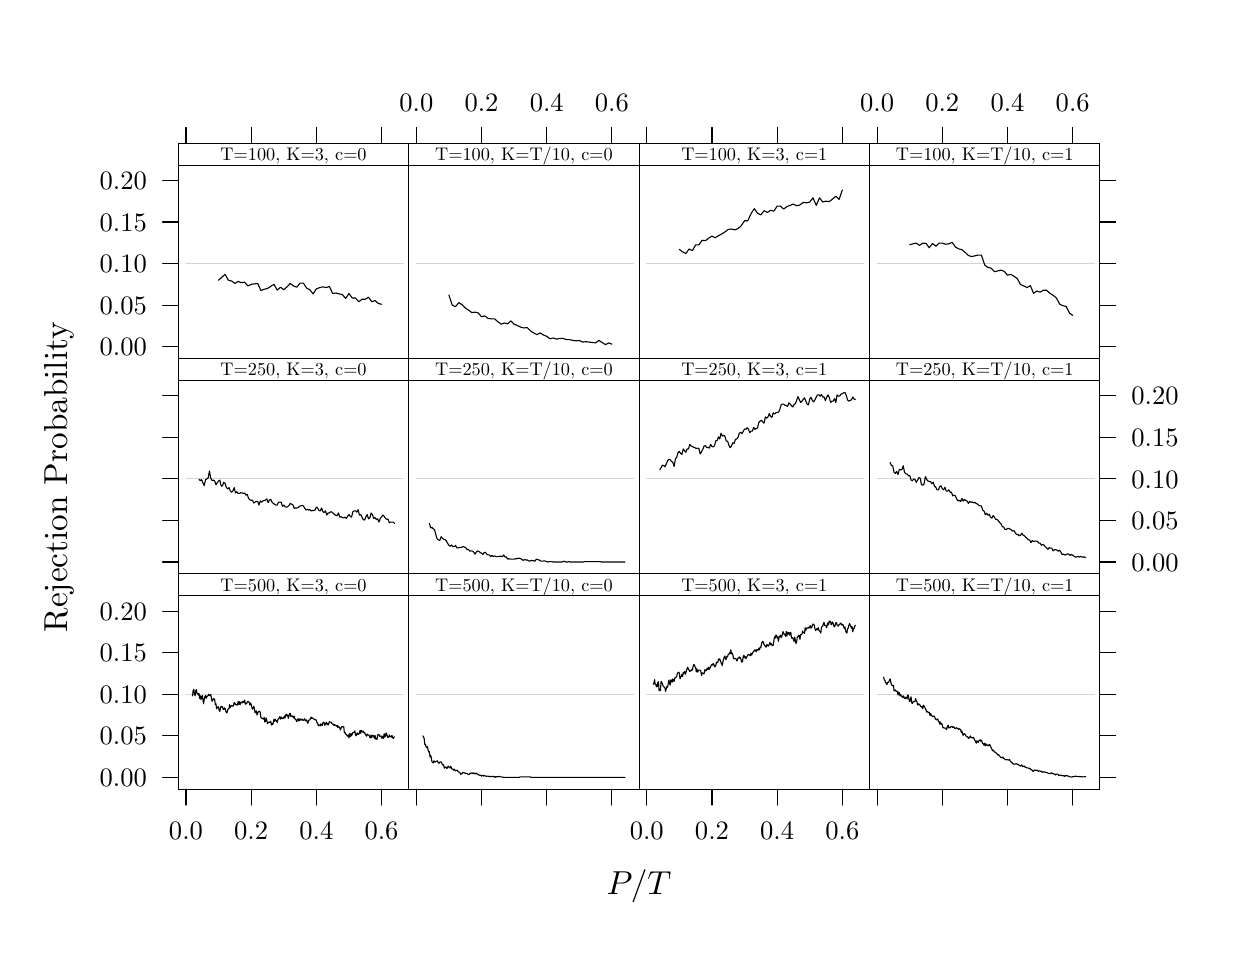
\begin{tikzpicture}[x=1pt,y=1pt]
\definecolor[named]{fillColor}{rgb}{1.00,1.00,1.00}
\path[use as bounding box,fill=fillColor,fill opacity=0.00] (0,0) rectangle (433.62,325.21);
\begin{scope}
\path[clip] (  0.00,  0.00) rectangle (433.62,325.21);

\path[] (  0.00,  0.00) rectangle (433.62,325.21);
\definecolor[named]{drawColor}{rgb}{0.00,0.00,0.00}

\node[text=drawColor,anchor=base,inner sep=0pt, outer sep=0pt, scale=  1.20] at (220.94, 12.05) {$P/T$};
\end{scope}
\begin{scope}
\path[clip] (  0.00,  0.00) rectangle (433.62,325.21);
\definecolor[named]{drawColor}{rgb}{0.00,0.00,0.00}

\node[text=drawColor,rotate= 90.00,anchor=base,inner sep=0pt, outer sep=0pt, scale=  1.20] at ( 14.29,162.76) {Rejection Probability};
\end{scope}
\begin{scope}
\path[clip] (  0.00,  0.00) rectangle (433.62,325.21);
\definecolor[named]{drawColor}{rgb}{0.00,0.00,0.00}

\path[draw=drawColor,line width= 0.4pt,line join=round,line cap=round] ( 54.44, 54.31) -- ( 48.75, 54.31);

\path[draw=drawColor,line width= 0.4pt,line join=round,line cap=round] ( 54.44, 69.33) -- ( 48.75, 69.33);

\path[draw=drawColor,line width= 0.4pt,line join=round,line cap=round] ( 54.44, 84.35) -- ( 48.75, 84.35);

\path[draw=drawColor,line width= 0.4pt,line join=round,line cap=round] ( 54.44, 99.37) -- ( 48.75, 99.37);

\path[draw=drawColor,line width= 0.4pt,line join=round,line cap=round] ( 54.44,114.39) -- ( 48.75,114.39);

\node[text=drawColor,anchor=base east,inner sep=0pt, outer sep=0pt, scale=  0.96] at ( 43.06, 51.00) {0.00};

\node[text=drawColor,anchor=base east,inner sep=0pt, outer sep=0pt, scale=  0.96] at ( 43.06, 66.02) {0.05};

\node[text=drawColor,anchor=base east,inner sep=0pt, outer sep=0pt, scale=  0.96] at ( 43.06, 81.04) {0.10};

\node[text=drawColor,anchor=base east,inner sep=0pt, outer sep=0pt, scale=  0.96] at ( 43.06, 96.06) {0.15};

\node[text=drawColor,anchor=base east,inner sep=0pt, outer sep=0pt, scale=  0.96] at ( 43.06,111.08) {0.20};
\end{scope}
\begin{scope}
\path[clip] (  0.00,  0.00) rectangle (433.62,325.21);
\definecolor[named]{drawColor}{rgb}{0.00,0.00,0.00}

\path[draw=drawColor,line width= 0.4pt,line join=round,line cap=round] ( 57.20, 50.02) -- ( 57.20, 44.32);

\path[draw=drawColor,line width= 0.4pt,line join=round,line cap=round] ( 80.76, 50.02) -- ( 80.76, 44.32);

\path[draw=drawColor,line width= 0.4pt,line join=round,line cap=round] (104.31, 50.02) -- (104.31, 44.32);

\path[draw=drawColor,line width= 0.4pt,line join=round,line cap=round] (127.87, 50.02) -- (127.87, 44.32);

\node[text=drawColor,anchor=base,inner sep=0pt, outer sep=0pt, scale=  0.96] at ( 57.20, 32.02) {0.0};

\node[text=drawColor,anchor=base,inner sep=0pt, outer sep=0pt, scale=  0.96] at ( 80.76, 32.02) {0.2};

\node[text=drawColor,anchor=base,inner sep=0pt, outer sep=0pt, scale=  0.96] at (104.31, 32.02) {0.4};

\node[text=drawColor,anchor=base,inner sep=0pt, outer sep=0pt, scale=  0.96] at (127.87, 32.02) {0.6};
\end{scope}
\begin{scope}
\path[clip] ( 54.44, 50.02) rectangle (137.69,119.88);
\definecolor[named]{drawColor}{rgb}{0.83,0.83,0.83}

\path[draw=drawColor,line width= 0.4pt,line join=round,line cap=round] ( 57.20, 84.35) --
	(135.72, 84.35);
\definecolor[named]{drawColor}{rgb}{0.00,0.00,0.00}

\path[draw=drawColor,line width= 0.4pt,line join=round,line cap=round] ( 59.56, 83.75) --
	( 59.79, 85.70) --
	( 60.03, 86.15) --
	( 60.26, 84.35) --
	( 60.50, 83.75) --
	( 60.73, 85.70) --
	( 60.97, 86.00) --
	( 61.20, 84.65) --
	( 61.44, 84.50) --
	( 61.68, 84.05) --
	( 61.91, 84.65) --
	( 62.15, 82.85) --
	( 62.38, 83.75) --
	( 62.62, 82.40) --
	( 62.85, 83.45) --
	( 63.09, 83.90) --
	( 63.32, 82.40) --
	( 63.56, 80.89) --
	( 63.80, 82.55) --
	( 64.03, 83.45) --
	( 64.27, 83.90) --
	( 64.50, 82.85) --
	( 64.74, 83.60) --
	( 64.97, 83.60) --
	( 65.21, 83.90) --
	( 65.44, 84.35) --
	( 65.68, 83.90) --
	( 65.92, 83.90) --
	( 66.15, 84.20) --
	( 66.39, 83.00) --
	( 66.62, 81.79) --
	( 66.86, 82.09) --
	( 67.09, 82.70) --
	( 67.33, 82.70) --
	( 67.56, 82.55) --
	( 67.80, 80.59) --
	( 68.04, 80.89) --
	( 68.27, 79.09) --
	( 68.51, 79.54) --
	( 68.74, 79.84) --
	( 68.98, 79.69) --
	( 69.21, 78.34) --
	( 69.45, 78.19) --
	( 69.69, 79.54) --
	( 69.92, 79.99) --
	( 70.16, 79.69) --
	( 70.39, 79.84) --
	( 70.63, 78.94) --
	( 70.86, 78.79) --
	( 71.10, 79.39) --
	( 71.33, 79.24) --
	( 71.57, 78.34) --
	( 71.81, 77.59) --
	( 72.04, 77.74) --
	( 72.28, 78.64) --
	( 72.51, 79.09) --
	( 72.75, 79.09) --
	( 72.98, 80.59) --
	( 73.22, 79.54) --
	( 73.45, 79.99) --
	( 73.69, 80.29) --
	( 73.93, 80.14) --
	( 74.16, 79.99) --
	( 74.40, 80.29) --
	( 74.63, 81.34) --
	( 74.87, 81.19) --
	( 75.10, 80.59) --
	( 75.34, 80.74) --
	( 75.57, 80.44) --
	( 75.81, 80.44) --
	( 76.05, 81.79) --
	( 76.28, 80.74) --
	( 76.52, 81.64) --
	( 76.75, 80.59) --
	( 76.99, 81.34) --
	( 77.22, 81.49) --
	( 77.46, 81.19) --
	( 77.69, 81.79) --
	( 77.93, 81.79) --
	( 78.17, 81.34) --
	( 78.40, 82.24) --
	( 78.64, 80.74) --
	( 78.87, 81.04) --
	( 79.11, 80.89) --
	( 79.34, 81.49) --
	( 79.58, 81.79) --
	( 79.81, 81.64) --
	( 80.05, 81.34) --
	( 80.29, 80.44) --
	( 80.52, 81.19) --
	( 80.76, 80.74) --
	( 80.99, 79.69) --
	( 81.23, 78.94) --
	( 81.46, 79.24) --
	( 81.70, 79.99) --
	( 81.93, 79.09) --
	( 82.17, 77.59) --
	( 82.41, 78.19) --
	( 82.64, 78.34) --
	( 82.88, 76.84) --
	( 83.11, 77.44) --
	( 83.35, 78.04) --
	( 83.58, 78.19) --
	( 83.82, 78.19) --
	( 84.05, 77.74) --
	( 84.29, 75.79) --
	( 84.53, 75.79) --
	( 84.76, 75.49) --
	( 85.00, 75.64) --
	( 85.23, 75.34) --
	( 85.47, 75.94) --
	( 85.70, 74.28) --
	( 85.94, 74.58) --
	( 86.17, 75.79) --
	( 86.41, 74.88) --
	( 86.65, 73.83) --
	( 86.88, 73.98) --
	( 87.12, 74.28) --
	( 87.35, 74.13) --
	( 87.59, 74.28) --
	( 87.82, 74.58) --
	( 88.06, 73.23) --
	( 88.29, 73.83) --
	( 88.53, 73.38) --
	( 88.77, 74.13) --
	( 89.00, 75.34) --
	( 89.24, 74.58) --
	( 89.47, 75.34) --
	( 89.71, 74.88) --
	( 89.94, 74.73) --
	( 90.18, 74.13) --
	( 90.41, 75.19) --
	( 90.65, 75.49) --
	( 90.89, 75.79) --
	( 91.12, 76.24) --
	( 91.36, 75.34) --
	( 91.59, 76.09) --
	( 91.83, 75.94) --
	( 92.06, 75.49) --
	( 92.30, 75.79) --
	( 92.53, 75.64) --
	( 92.77, 76.54) --
	( 93.01, 75.79) --
	( 93.24, 76.84) --
	( 93.48, 77.14) --
	( 93.71, 76.54) --
	( 93.95, 76.84) --
	( 94.18, 75.64) --
	( 94.42, 76.54) --
	( 94.66, 77.44) --
	( 94.89, 77.44) --
	( 95.13, 76.24) --
	( 95.36, 76.39) --
	( 95.60, 76.54) --
	( 95.83, 76.39) --
	( 96.07, 75.79) --
	( 96.30, 76.39) --
	( 96.54, 75.49) --
	( 96.78, 75.19) --
	( 97.01, 75.03) --
	( 97.25, 74.43) --
	( 97.48, 75.19) --
	( 97.72, 75.49) --
	( 97.95, 74.73) --
	( 98.19, 74.88) --
	( 98.42, 75.49) --
	( 98.66, 75.03) --
	( 98.90, 75.03) --
	( 99.13, 75.34) --
	( 99.37, 75.03) --
	( 99.60, 74.88) --
	( 99.84, 75.19) --
	(100.07, 75.49) --
	(100.31, 74.73) --
	(100.54, 75.03) --
	(100.78, 75.03) --
	(101.02, 74.28) --
	(101.25, 73.83) --
	(101.49, 74.88) --
	(101.72, 75.03) --
	(101.96, 75.03) --
	(102.19, 75.64) --
	(102.43, 76.09) --
	(102.66, 75.64) --
	(102.90, 75.79) --
	(103.14, 75.64) --
	(103.37, 75.34) --
	(103.61, 75.34) --
	(103.84, 75.03) --
	(104.08, 75.19) --
	(104.31, 74.88) --
	(104.55, 73.98) --
	(104.78, 73.98) --
	(105.02, 72.93) --
	(105.26, 73.23) --
	(105.49, 73.23) --
	(105.73, 72.93) --
	(105.96, 73.68) --
	(106.20, 73.23) --
	(106.43, 73.08) --
	(106.67, 73.98) --
	(106.90, 74.28) --
	(107.14, 73.98) --
	(107.38, 73.08) --
	(107.61, 73.53) --
	(107.85, 74.28) --
	(108.08, 73.53) --
	(108.32, 73.83) --
	(108.55, 73.23) --
	(108.79, 73.68) --
	(109.02, 74.43) --
	(109.26, 74.28) --
	(109.50, 74.28) --
	(109.73, 74.13) --
	(109.97, 73.68) --
	(110.20, 73.53) --
	(110.44, 73.53) --
	(110.67, 73.08) --
	(110.91, 73.38) --
	(111.14, 73.08) --
	(111.38, 73.08) --
	(111.62, 72.78) --
	(111.85, 73.08) --
	(112.09, 72.33) --
	(112.32, 72.78) --
	(112.56, 72.48) --
	(112.79, 72.18) --
	(113.03, 71.43) --
	(113.26, 72.18) --
	(113.50, 72.63) --
	(113.74, 72.63) --
	(113.97, 72.48) --
	(114.21, 72.63) --
	(114.44, 70.38) --
	(114.68, 70.53) --
	(114.91, 69.93) --
	(115.15, 69.78) --
	(115.38, 69.48) --
	(115.62, 69.18) --
	(115.86, 69.63) --
	(116.09, 68.58) --
	(116.33, 70.08) --
	(116.56, 69.03) --
	(116.80, 70.08) --
	(117.03, 69.33) --
	(117.27, 69.93) --
	(117.51, 70.53) --
	(117.74, 70.53) --
	(117.98, 70.53) --
	(118.21, 71.13) --
	(118.45, 69.78) --
	(118.68, 69.33) --
	(118.92, 70.08) --
	(119.15, 70.38) --
	(119.39, 69.78) --
	(119.63, 69.93) --
	(119.86, 70.23) --
	(120.10, 71.28) --
	(120.33, 70.23) --
	(120.57, 71.28) --
	(120.80, 70.98) --
	(121.04, 70.68) --
	(121.27, 70.98) --
	(121.51, 70.38) --
	(121.75, 70.53) --
	(121.98, 69.93) --
	(122.22, 69.63) --
	(122.45, 69.18) --
	(122.69, 69.93) --
	(122.92, 69.63) --
	(123.16, 69.63) --
	(123.39, 69.48) --
	(123.63, 68.73) --
	(123.87, 68.58) --
	(124.10, 69.63) --
	(124.34, 68.73) --
	(124.57, 69.33) --
	(124.81, 69.48) --
	(125.04, 69.18) --
	(125.28, 68.43) --
	(125.51, 69.48) --
	(125.75, 68.13) --
	(125.99, 68.43) --
	(126.22, 67.97) --
	(126.46, 69.63) --
	(126.69, 69.78) --
	(126.93, 69.78) --
	(127.16, 69.18) --
	(127.40, 69.18) --
	(127.63, 69.33) --
	(127.87, 68.58) --
	(128.11, 68.43) --
	(128.34, 69.18) --
	(128.58, 68.43) --
	(128.81, 70.08) --
	(129.05, 68.88) --
	(129.28, 69.33) --
	(129.52, 70.38) --
	(129.75, 69.93) --
	(129.99, 69.03) --
	(130.23, 68.73) --
	(130.46, 68.88) --
	(130.70, 69.63) --
	(130.93, 69.03) --
	(131.17, 69.18) --
	(131.40, 68.88) --
	(131.64, 69.48) --
	(131.87, 68.58) --
	(132.11, 68.43) --
	(132.35, 68.88) --
	(132.58, 68.88);
\end{scope}
\begin{scope}
\path[clip] (  0.00,  0.00) rectangle (433.62,325.21);
\definecolor[named]{drawColor}{rgb}{0.00,0.00,0.00}

\path[draw=drawColor,line width= 0.4pt,line join=round,line cap=round] ( 54.44, 50.02) rectangle (137.69,119.88);
\end{scope}
\begin{scope}
\path[clip] ( 54.44,119.88) rectangle (137.69,127.83);

\path[] ( 54.44,119.88) rectangle (137.69,127.83);
\definecolor[named]{drawColor}{rgb}{0.00,0.00,0.00}

\node[text=drawColor,anchor=base west,inner sep=0pt, outer sep=0pt, scale=  0.66] at ( 69.67,121.58) {T=500, K=3, c=0};
\end{scope}
\begin{scope}
\path[clip] (  0.00,  0.00) rectangle (433.62,325.21);
\definecolor[named]{drawColor}{rgb}{0.00,0.00,0.00}

\path[draw=drawColor,line width= 0.4pt,line join=round,line cap=round] ( 54.44,119.88) rectangle (137.69,127.83);
\end{scope}
\begin{scope}
\path[clip] (  0.00,  0.00) rectangle (433.62,325.21);
\definecolor[named]{drawColor}{rgb}{0.00,0.00,0.00}

\path[draw=drawColor,line width= 0.4pt,line join=round,line cap=round] (140.45, 50.02) -- (140.45, 44.32);

\path[draw=drawColor,line width= 0.4pt,line join=round,line cap=round] (164.01, 50.02) -- (164.01, 44.32);

\path[draw=drawColor,line width= 0.4pt,line join=round,line cap=round] (187.56, 50.02) -- (187.56, 44.32);

\path[draw=drawColor,line width= 0.4pt,line join=round,line cap=round] (211.12, 50.02) -- (211.12, 44.32);
\end{scope}
\begin{scope}
\path[clip] (137.69, 50.02) rectangle (220.94,119.88);
\definecolor[named]{drawColor}{rgb}{0.83,0.83,0.83}

\path[draw=drawColor,line width= 0.4pt,line join=round,line cap=round] (140.45, 84.35) --
	(218.97, 84.35);
\definecolor[named]{drawColor}{rgb}{0.00,0.00,0.00}

\path[draw=drawColor,line width= 0.4pt,line join=round,line cap=round] (142.80, 69.33) --
	(143.04, 68.88) --
	(143.28, 68.28) --
	(143.51, 66.17) --
	(143.75, 66.17) --
	(143.98, 65.27) --
	(144.22, 65.12) --
	(144.45, 65.42) --
	(144.69, 64.22) --
	(144.92, 63.47) --
	(145.16, 63.62) --
	(145.40, 61.67) --
	(145.63, 62.27) --
	(145.87, 61.22) --
	(146.10, 59.86) --
	(146.34, 59.71) --
	(146.57, 59.56) --
	(146.81, 60.31) --
	(147.05, 59.86) --
	(147.28, 59.86) --
	(147.52, 60.01) --
	(147.75, 60.16) --
	(147.99, 60.31) --
	(148.22, 59.86) --
	(148.46, 59.56) --
	(148.69, 59.41) --
	(148.93, 59.86) --
	(149.17, 59.86) --
	(149.40, 59.86) --
	(149.64, 59.56) --
	(149.87, 58.81) --
	(150.11, 58.96) --
	(150.34, 58.66) --
	(150.58, 57.61) --
	(150.81, 58.06) --
	(151.05, 57.91) --
	(151.29, 57.91) --
	(151.52, 57.46) --
	(151.76, 58.06) --
	(151.99, 58.36) --
	(152.23, 58.06) --
	(152.46, 57.76) --
	(152.70, 57.76) --
	(152.93, 58.36) --
	(153.17, 57.46) --
	(153.41, 57.31) --
	(153.64, 57.31) --
	(153.88, 56.86) --
	(154.11, 57.31) --
	(154.35, 57.01) --
	(154.58, 56.71) --
	(154.82, 56.71) --
	(155.05, 56.86) --
	(155.29, 56.86) --
	(155.53, 56.41) --
	(155.76, 56.26) --
	(156.00, 56.11) --
	(156.23, 55.96) --
	(156.47, 55.36) --
	(156.70, 55.66) --
	(156.94, 55.66) --
	(157.17, 55.96) --
	(157.41, 56.11) --
	(157.65, 55.96) --
	(157.88, 55.81) --
	(158.12, 55.96) --
	(158.35, 55.66) --
	(158.59, 55.66) --
	(158.82, 55.66) --
	(159.06, 55.51) --
	(159.29, 55.36) --
	(159.53, 55.36) --
	(159.77, 55.66) --
	(160.00, 55.81) --
	(160.24, 55.96) --
	(160.47, 55.81) --
	(160.71, 55.66) --
	(160.94, 55.96) --
	(161.18, 55.81) --
	(161.41, 55.81) --
	(161.65, 55.51) --
	(161.89, 55.81) --
	(162.12, 55.81) --
	(162.36, 55.51) --
	(162.59, 55.51) --
	(162.83, 55.21) --
	(163.06, 55.21) --
	(163.30, 55.06) --
	(163.53, 55.06) --
	(163.77, 55.06) --
	(164.01, 54.76) --
	(164.24, 55.06) --
	(164.48, 54.91) --
	(164.71, 54.76) --
	(164.95, 55.06) --
	(165.18, 54.91) --
	(165.42, 54.76) --
	(165.65, 54.76) --
	(165.89, 54.61) --
	(166.13, 54.76) --
	(166.36, 54.76) --
	(166.60, 54.61) --
	(166.83, 54.61) --
	(167.07, 54.61) --
	(167.30, 54.61) --
	(167.54, 54.61) --
	(167.77, 54.61) --
	(168.01, 54.61) --
	(168.25, 54.61) --
	(168.48, 54.61) --
	(168.72, 54.46) --
	(168.95, 54.31) --
	(169.19, 54.61) --
	(169.42, 54.46) --
	(169.66, 54.61) --
	(169.90, 54.46) --
	(170.13, 54.61) --
	(170.37, 54.61) --
	(170.60, 54.61) --
	(170.84, 54.46) --
	(171.07, 54.46) --
	(171.31, 54.46) --
	(171.54, 54.46) --
	(171.78, 54.31) --
	(172.02, 54.31) --
	(172.25, 54.31) --
	(172.49, 54.31) --
	(172.72, 54.31) --
	(172.96, 54.31) --
	(173.19, 54.31) --
	(173.43, 54.31) --
	(173.66, 54.31) --
	(173.90, 54.31) --
	(174.14, 54.31) --
	(174.37, 54.31) --
	(174.61, 54.31) --
	(174.84, 54.31) --
	(175.08, 54.31) --
	(175.31, 54.31) --
	(175.55, 54.31) --
	(175.78, 54.31) --
	(176.02, 54.31) --
	(176.26, 54.31) --
	(176.49, 54.31) --
	(176.73, 54.31) --
	(176.96, 54.31) --
	(177.20, 54.31) --
	(177.43, 54.31) --
	(177.67, 54.31) --
	(177.90, 54.46) --
	(178.14, 54.46) --
	(178.38, 54.46) --
	(178.61, 54.46) --
	(178.85, 54.46) --
	(179.08, 54.46) --
	(179.32, 54.46) --
	(179.55, 54.46) --
	(179.79, 54.46) --
	(180.02, 54.46) --
	(180.26, 54.46) --
	(180.50, 54.46) --
	(180.73, 54.46) --
	(180.97, 54.46) --
	(181.20, 54.46) --
	(181.44, 54.46) --
	(181.67, 54.46) --
	(181.91, 54.31) --
	(182.14, 54.31) --
	(182.38, 54.31) --
	(182.62, 54.31) --
	(182.85, 54.31) --
	(183.09, 54.31) --
	(183.32, 54.31) --
	(183.56, 54.31) --
	(183.79, 54.31) --
	(184.03, 54.31) --
	(184.26, 54.31) --
	(184.50, 54.31) --
	(184.74, 54.31) --
	(184.97, 54.31) --
	(185.21, 54.31) --
	(185.44, 54.31) --
	(185.68, 54.31) --
	(185.91, 54.31) --
	(186.15, 54.31) --
	(186.38, 54.31) --
	(186.62, 54.31) --
	(186.86, 54.31) --
	(187.09, 54.31) --
	(187.33, 54.31) --
	(187.56, 54.31) --
	(187.80, 54.31) --
	(188.03, 54.31) --
	(188.27, 54.31) --
	(188.50, 54.31) --
	(188.74, 54.31) --
	(188.98, 54.31) --
	(189.21, 54.31) --
	(189.45, 54.31) --
	(189.68, 54.31) --
	(189.92, 54.31) --
	(190.15, 54.31) --
	(190.39, 54.31) --
	(190.62, 54.31) --
	(190.86, 54.31) --
	(191.10, 54.31) --
	(191.33, 54.31) --
	(191.57, 54.31) --
	(191.80, 54.31) --
	(192.04, 54.31) --
	(192.27, 54.31) --
	(192.51, 54.31) --
	(192.74, 54.31) --
	(192.98, 54.31) --
	(193.22, 54.31) --
	(193.45, 54.31) --
	(193.69, 54.31) --
	(193.92, 54.31) --
	(194.16, 54.31) --
	(194.39, 54.31) --
	(194.63, 54.31) --
	(194.87, 54.31) --
	(195.10, 54.31) --
	(195.34, 54.31) --
	(195.57, 54.31) --
	(195.81, 54.31) --
	(196.04, 54.31) --
	(196.28, 54.31) --
	(196.51, 54.31) --
	(196.75, 54.31) --
	(196.99, 54.31) --
	(197.22, 54.31) --
	(197.46, 54.31) --
	(197.69, 54.31) --
	(197.93, 54.31) --
	(198.16, 54.31) --
	(198.40, 54.31) --
	(198.63, 54.31) --
	(198.87, 54.31) --
	(199.11, 54.31) --
	(199.34, 54.31) --
	(199.58, 54.31) --
	(199.81, 54.31) --
	(200.05, 54.31) --
	(200.28, 54.31) --
	(200.52, 54.31) --
	(200.75, 54.31) --
	(200.99, 54.31) --
	(201.23, 54.31) --
	(201.46, 54.31) --
	(201.70, 54.31) --
	(201.93, 54.31) --
	(202.17, 54.31) --
	(202.40, 54.31) --
	(202.64, 54.31) --
	(202.87, 54.31) --
	(203.11, 54.31) --
	(203.35, 54.31) --
	(203.58, 54.31) --
	(203.82, 54.31) --
	(204.05, 54.31) --
	(204.29, 54.31) --
	(204.52, 54.31) --
	(204.76, 54.31) --
	(204.99, 54.31) --
	(205.23, 54.31) --
	(205.47, 54.31) --
	(205.70, 54.31) --
	(205.94, 54.31) --
	(206.17, 54.31) --
	(206.41, 54.31) --
	(206.64, 54.31) --
	(206.88, 54.31) --
	(207.11, 54.31) --
	(207.35, 54.31) --
	(207.59, 54.31) --
	(207.82, 54.31) --
	(208.06, 54.31) --
	(208.29, 54.31) --
	(208.53, 54.31) --
	(208.76, 54.31) --
	(209.00, 54.31) --
	(209.23, 54.31) --
	(209.47, 54.31) --
	(209.71, 54.31) --
	(209.94, 54.31) --
	(210.18, 54.31) --
	(210.41, 54.31) --
	(210.65, 54.31) --
	(210.88, 54.31) --
	(211.12, 54.31) --
	(211.35, 54.31) --
	(211.59, 54.31) --
	(211.83, 54.31) --
	(212.06, 54.31) --
	(212.30, 54.31) --
	(212.53, 54.31) --
	(212.77, 54.31) --
	(213.00, 54.31) --
	(213.24, 54.31) --
	(213.47, 54.31) --
	(213.71, 54.31) --
	(213.95, 54.31) --
	(214.18, 54.31) --
	(214.42, 54.31) --
	(214.65, 54.31) --
	(214.89, 54.31) --
	(215.12, 54.31) --
	(215.36, 54.31) --
	(215.59, 54.31) --
	(215.83, 54.31);
\end{scope}
\begin{scope}
\path[clip] (  0.00,  0.00) rectangle (433.62,325.21);
\definecolor[named]{drawColor}{rgb}{0.00,0.00,0.00}

\path[draw=drawColor,line width= 0.4pt,line join=round,line cap=round] (137.69, 50.02) rectangle (220.94,119.88);
\end{scope}
\begin{scope}
\path[clip] (137.69,119.88) rectangle (220.94,127.83);

\path[] (137.69,119.88) rectangle (220.94,127.83);
\definecolor[named]{drawColor}{rgb}{0.00,0.00,0.00}

\node[text=drawColor,anchor=base west,inner sep=0pt, outer sep=0pt, scale=  0.66] at (147.24,121.58) {T=500, K=T/10, c=0};
\end{scope}
\begin{scope}
\path[clip] (  0.00,  0.00) rectangle (433.62,325.21);
\definecolor[named]{drawColor}{rgb}{0.00,0.00,0.00}

\path[draw=drawColor,line width= 0.4pt,line join=round,line cap=round] (137.69,119.88) rectangle (220.94,127.83);
\end{scope}
\begin{scope}
\path[clip] (  0.00,  0.00) rectangle (433.62,325.21);
\definecolor[named]{drawColor}{rgb}{0.00,0.00,0.00}

\path[draw=drawColor,line width= 0.4pt,line join=round,line cap=round] (223.70, 50.02) -- (223.70, 44.32);

\path[draw=drawColor,line width= 0.4pt,line join=round,line cap=round] (247.26, 50.02) -- (247.26, 44.32);

\path[draw=drawColor,line width= 0.4pt,line join=round,line cap=round] (270.81, 50.02) -- (270.81, 44.32);

\path[draw=drawColor,line width= 0.4pt,line join=round,line cap=round] (294.37, 50.02) -- (294.37, 44.32);

\node[text=drawColor,anchor=base,inner sep=0pt, outer sep=0pt, scale=  0.96] at (223.70, 32.02) {0.0};

\node[text=drawColor,anchor=base,inner sep=0pt, outer sep=0pt, scale=  0.96] at (247.26, 32.02) {0.2};

\node[text=drawColor,anchor=base,inner sep=0pt, outer sep=0pt, scale=  0.96] at (270.81, 32.02) {0.4};

\node[text=drawColor,anchor=base,inner sep=0pt, outer sep=0pt, scale=  0.96] at (294.37, 32.02) {0.6};
\end{scope}
\begin{scope}
\path[clip] (220.94, 50.02) rectangle (304.19,119.88);
\definecolor[named]{drawColor}{rgb}{0.83,0.83,0.83}

\path[draw=drawColor,line width= 0.4pt,line join=round,line cap=round] (223.70, 84.35) --
	(302.22, 84.35);
\definecolor[named]{drawColor}{rgb}{0.00,0.00,0.00}

\path[draw=drawColor,line width= 0.4pt,line join=round,line cap=round] (226.05, 87.95) --
	(226.29, 88.40) --
	(226.53, 89.61) --
	(226.76, 87.80) --
	(227.00, 87.95) --
	(227.23, 87.05) --
	(227.47, 87.05) --
	(227.70, 88.70) --
	(227.94, 88.85) --
	(228.17, 85.55) --
	(228.41, 86.15) --
	(228.65, 85.70) --
	(228.88, 89.00) --
	(229.12, 88.70) --
	(229.35, 88.10) --
	(229.59, 87.35) --
	(229.82, 87.20) --
	(230.06, 86.75) --
	(230.29, 86.60) --
	(230.53, 85.40) --
	(230.77, 86.45) --
	(231.00, 87.20) --
	(231.24, 86.90) --
	(231.47, 88.25) --
	(231.71, 89.46) --
	(231.94, 88.25) --
	(232.18, 87.65) --
	(232.41, 89.61) --
	(232.65, 89.15) --
	(232.89, 88.70) --
	(233.12, 89.91) --
	(233.36, 89.15) --
	(233.59, 89.00) --
	(233.83, 90.21) --
	(234.06, 90.36) --
	(234.30, 90.51) --
	(234.53, 90.81) --
	(234.77, 92.01) --
	(235.01, 92.01) --
	(235.24, 92.31) --
	(235.48, 92.01) --
	(235.71, 89.91) --
	(235.95, 90.51) --
	(236.18, 90.81) --
	(236.42, 91.56) --
	(236.65, 90.81) --
	(236.89, 92.16) --
	(237.13, 92.01) --
	(237.36, 92.61) --
	(237.60, 91.56) --
	(237.83, 92.01) --
	(238.07, 93.06) --
	(238.30, 93.66) --
	(238.54, 94.11) --
	(238.77, 93.36) --
	(239.01, 93.06) --
	(239.25, 92.61) --
	(239.48, 92.91) --
	(239.72, 92.76) --
	(239.95, 93.21) --
	(240.19, 93.06) --
	(240.42, 94.26) --
	(240.66, 95.01) --
	(240.89, 95.01) --
	(241.13, 94.26) --
	(241.37, 93.96) --
	(241.60, 92.46) --
	(241.84, 93.51) --
	(242.07, 92.31) --
	(242.31, 92.76) --
	(242.54, 93.06) --
	(242.78, 93.06) --
	(243.01, 93.06) --
	(243.25, 92.61) --
	(243.49, 91.11) --
	(243.72, 92.01) --
	(243.96, 92.01) --
	(244.19, 91.71) --
	(244.43, 91.71) --
	(244.66, 93.21) --
	(244.90, 92.91) --
	(245.13, 92.76) --
	(245.37, 93.51) --
	(245.61, 93.81) --
	(245.84, 93.21) --
	(246.08, 94.11) --
	(246.31, 93.36) --
	(246.55, 93.81) --
	(246.78, 94.26) --
	(247.02, 94.86) --
	(247.26, 95.16) --
	(247.49, 94.86) --
	(247.73, 95.46) --
	(247.96, 95.16) --
	(248.20, 94.26) --
	(248.43, 94.41) --
	(248.67, 94.71) --
	(248.90, 95.91) --
	(249.14, 95.76) --
	(249.38, 95.91) --
	(249.61, 97.12) --
	(249.85, 96.67) --
	(250.08, 97.12) --
	(250.32, 96.52) --
	(250.55, 95.76) --
	(250.79, 95.16) --
	(251.02, 94.71) --
	(251.26, 96.36) --
	(251.50, 97.12) --
	(251.73, 97.87) --
	(251.97, 98.17) --
	(252.20, 96.97) --
	(252.44, 96.97) --
	(252.67, 98.02) --
	(252.91, 97.87) --
	(253.14, 98.77) --
	(253.38, 98.77) --
	(253.62, 99.37) --
	(253.85, 99.07) --
	(254.09,100.42) --
	(254.32, 98.92) --
	(254.56, 99.22) --
	(254.79, 98.62) --
	(255.03, 97.42) --
	(255.26, 97.12) --
	(255.50, 97.27) --
	(255.74, 97.27) --
	(255.97, 97.12) --
	(256.21, 96.36) --
	(256.44, 96.67) --
	(256.68, 97.42) --
	(256.91, 97.42) --
	(257.15, 97.87) --
	(257.38, 97.27) --
	(257.62, 97.57) --
	(257.86, 96.36) --
	(258.09, 95.91) --
	(258.33, 96.36) --
	(258.56, 97.87) --
	(258.80, 98.47) --
	(259.03, 97.57) --
	(259.27, 98.02) --
	(259.50, 97.27) --
	(259.74, 97.42) --
	(259.98, 98.17) --
	(260.21, 98.47) --
	(260.45, 98.77) --
	(260.68, 98.62) --
	(260.92, 98.32) --
	(261.15, 98.32) --
	(261.39, 99.22) --
	(261.62, 98.47) --
	(261.86, 99.07) --
	(262.10, 99.52) --
	(262.33, 99.97) --
	(262.57, 99.97) --
	(262.80,100.42) --
	(263.04,100.12) --
	(263.27, 99.67) --
	(263.51,100.57) --
	(263.74,100.27) --
	(263.98,100.27) --
	(264.22,101.02) --
	(264.45,100.42) --
	(264.69,101.32) --
	(264.92,101.17) --
	(265.16,102.37) --
	(265.39,103.27) --
	(265.63,103.42) --
	(265.86,103.12) --
	(266.10,102.22) --
	(266.34,101.92) --
	(266.57,101.62) --
	(266.81,101.32) --
	(267.04,102.22) --
	(267.28,102.22) --
	(267.51,101.77) --
	(267.75,101.77) --
	(267.98,102.52) --
	(268.22,103.12) --
	(268.46,102.22) --
	(268.69,102.67) --
	(268.93,102.07) --
	(269.16,101.92) --
	(269.40,102.07) --
	(269.63,103.58) --
	(269.87,105.08) --
	(270.11,104.63) --
	(270.34,105.68) --
	(270.58,105.68) --
	(270.81,104.63) --
	(271.05,105.08) --
	(271.28,103.42) --
	(271.52,104.93) --
	(271.75,105.23) --
	(271.99,105.68) --
	(272.23,104.78) --
	(272.46,105.08) --
	(272.70,105.98) --
	(272.93,107.03) --
	(273.17,106.13) --
	(273.40,106.13) --
	(273.64,105.83) --
	(273.87,105.23) --
	(274.11,107.03) --
	(274.35,105.38) --
	(274.58,106.73) --
	(274.82,106.13) --
	(275.05,106.58) --
	(275.29,105.68) --
	(275.52,106.58) --
	(275.76,106.73) --
	(275.99,104.63) --
	(276.23,104.78) --
	(276.47,104.78) --
	(276.70,104.03) --
	(276.94,103.42) --
	(277.17,104.93) --
	(277.41,103.73) --
	(277.64,102.67) --
	(277.88,103.42) --
	(278.11,105.08) --
	(278.35,105.08) --
	(278.59,105.68) --
	(278.82,105.53) --
	(279.06,104.18) --
	(279.29,105.83) --
	(279.53,105.98) --
	(279.76,105.98) --
	(280.00,107.18) --
	(280.23,106.58) --
	(280.47,106.73) --
	(280.71,106.28) --
	(280.94,108.38) --
	(281.18,107.48) --
	(281.41,108.08) --
	(281.65,108.38) --
	(281.88,108.23) --
	(282.12,108.53) --
	(282.35,108.23) --
	(282.59,108.68) --
	(282.83,109.13) --
	(283.06,108.23) --
	(283.30,108.38) --
	(283.53,109.13) --
	(283.77,109.73) --
	(284.00,109.58) --
	(284.24,109.28) --
	(284.47,108.08) --
	(284.71,107.33) --
	(284.95,107.63) --
	(285.18,108.08) --
	(285.42,107.63) --
	(285.65,108.38) --
	(285.89,107.48) --
	(286.12,107.18) --
	(286.36,107.03) --
	(286.59,106.43) --
	(286.83,108.53) --
	(287.07,108.83) --
	(287.30,108.98) --
	(287.54,109.88) --
	(287.77,110.33) --
	(288.01,109.13) --
	(288.24,109.13) --
	(288.48,109.13) --
	(288.71,108.38) --
	(288.95,109.58) --
	(289.19,110.18) --
	(289.42,109.43) --
	(289.66,110.79) --
	(289.89,110.79) --
	(290.13,110.48) --
	(290.36,109.43) --
	(290.60,109.88) --
	(290.83,110.48) --
	(291.07,109.88) --
	(291.31,108.98) --
	(291.54,108.68) --
	(291.78,109.28) --
	(292.01,110.18) --
	(292.25,110.18) --
	(292.48,109.43) --
	(292.72,109.13) --
	(292.96,108.98) --
	(293.19,109.58) --
	(293.43,109.58) --
	(293.66,109.88) --
	(293.90,110.03) --
	(294.13,109.43) --
	(294.37,109.28) --
	(294.60,109.58) --
	(294.84,108.83) --
	(295.08,108.08) --
	(295.31,108.68) --
	(295.55,107.33) --
	(295.78,106.73) --
	(296.02,106.43) --
	(296.25,107.93) --
	(296.49,108.23) --
	(296.72,109.13) --
	(296.96,109.88) --
	(297.20,109.43) --
	(297.43,108.83) --
	(297.67,108.23) --
	(297.90,108.83) --
	(298.14,106.88) --
	(298.37,108.08) --
	(298.61,108.08) --
	(298.84,108.83) --
	(299.08,109.28);
\end{scope}
\begin{scope}
\path[clip] (  0.00,  0.00) rectangle (433.62,325.21);
\definecolor[named]{drawColor}{rgb}{0.00,0.00,0.00}

\path[draw=drawColor,line width= 0.4pt,line join=round,line cap=round] (220.94, 50.02) rectangle (304.19,119.88);
\end{scope}
\begin{scope}
\path[clip] (220.94,119.88) rectangle (304.19,127.83);

\path[] (220.94,119.88) rectangle (304.19,127.83);
\definecolor[named]{drawColor}{rgb}{0.00,0.00,0.00}

\node[text=drawColor,anchor=base west,inner sep=0pt, outer sep=0pt, scale=  0.66] at (236.17,121.58) {T=500, K=3, c=1};
\end{scope}
\begin{scope}
\path[clip] (  0.00,  0.00) rectangle (433.62,325.21);
\definecolor[named]{drawColor}{rgb}{0.00,0.00,0.00}

\path[draw=drawColor,line width= 0.4pt,line join=round,line cap=round] (220.94,119.88) rectangle (304.19,127.83);
\end{scope}
\begin{scope}
\path[clip] (  0.00,  0.00) rectangle (433.62,325.21);
\definecolor[named]{drawColor}{rgb}{0.00,0.00,0.00}

\path[draw=drawColor,line width= 0.4pt,line join=round,line cap=round] (306.95, 50.02) -- (306.95, 44.32);

\path[draw=drawColor,line width= 0.4pt,line join=round,line cap=round] (330.50, 50.02) -- (330.50, 44.32);

\path[draw=drawColor,line width= 0.4pt,line join=round,line cap=round] (354.06, 50.02) -- (354.06, 44.32);

\path[draw=drawColor,line width= 0.4pt,line join=round,line cap=round] (377.62, 50.02) -- (377.62, 44.32);

\path[draw=drawColor,line width= 0.4pt,line join=round,line cap=round] (387.44, 54.31) -- (393.13, 54.31);

\path[draw=drawColor,line width= 0.4pt,line join=round,line cap=round] (387.44, 69.33) -- (393.13, 69.33);

\path[draw=drawColor,line width= 0.4pt,line join=round,line cap=round] (387.44, 84.35) -- (393.13, 84.35);

\path[draw=drawColor,line width= 0.4pt,line join=round,line cap=round] (387.44, 99.37) -- (393.13, 99.37);

\path[draw=drawColor,line width= 0.4pt,line join=round,line cap=round] (387.44,114.39) -- (393.13,114.39);
\end{scope}
\begin{scope}
\path[clip] (304.19, 50.02) rectangle (387.44,119.88);
\definecolor[named]{drawColor}{rgb}{0.83,0.83,0.83}

\path[draw=drawColor,line width= 0.4pt,line join=round,line cap=round] (306.95, 84.35) --
	(385.47, 84.35);
\definecolor[named]{drawColor}{rgb}{0.00,0.00,0.00}

\path[draw=drawColor,line width= 0.4pt,line join=round,line cap=round] (309.30, 90.50) --
	(309.54, 89.50) --
	(309.77, 89.34) --
	(310.01, 88.50) --
	(310.25, 88.42) --
	(310.48, 87.83) --
	(310.72, 88.67) --
	(310.95, 88.58) --
	(311.19, 88.92) --
	(311.42, 89.42) --
	(311.66, 89.92) --
	(311.89, 88.67) --
	(312.13, 87.83) --
	(312.37, 87.50) --
	(312.60, 87.33) --
	(312.84, 87.58) --
	(313.07, 85.58) --
	(313.31, 85.75) --
	(313.54, 85.92) --
	(313.78, 85.42) --
	(314.01, 85.42) --
	(314.25, 85.42) --
	(314.49, 84.08) --
	(314.72, 85.08) --
	(314.96, 84.92) --
	(315.19, 83.75) --
	(315.43, 84.25) --
	(315.66, 83.66) --
	(315.90, 83.58) --
	(316.13, 83.16) --
	(316.37, 83.75) --
	(316.61, 83.50) --
	(316.84, 82.75) --
	(317.08, 82.83) --
	(317.31, 83.25) --
	(317.55, 83.00) --
	(317.78, 82.66) --
	(318.02, 84.08) --
	(318.25, 83.75) --
	(318.49, 82.25) --
	(318.73, 81.66) --
	(318.96, 82.50) --
	(319.20, 83.41) --
	(319.43, 81.33) --
	(319.67, 81.00) --
	(319.90, 81.50) --
	(320.14, 81.75) --
	(320.37, 81.66) --
	(320.61, 81.66) --
	(320.85, 82.75) --
	(321.08, 82.08) --
	(321.32, 81.75) --
	(321.55, 80.49) --
	(321.79, 80.49) --
	(322.02, 80.91) --
	(322.26, 80.49) --
	(322.50, 80.41) --
	(322.73, 79.91) --
	(322.97, 79.66) --
	(323.20, 79.91) --
	(323.44, 79.16) --
	(323.67, 80.41) --
	(323.91, 80.08) --
	(324.14, 79.74) --
	(324.38, 79.08) --
	(324.62, 78.74) --
	(324.85, 77.91) --
	(325.09, 78.16) --
	(325.32, 77.91) --
	(325.56, 77.74) --
	(325.79, 77.83) --
	(326.03, 76.66) --
	(326.26, 77.41) --
	(326.50, 76.91) --
	(326.74, 76.49) --
	(326.97, 76.32) --
	(327.21, 76.24) --
	(327.44, 76.49) --
	(327.68, 76.41) --
	(327.91, 75.57) --
	(328.15, 75.24) --
	(328.38, 75.07) --
	(328.62, 75.32) --
	(328.86, 75.41) --
	(329.09, 74.49) --
	(329.33, 74.41) --
	(329.56, 73.57) --
	(329.80, 74.32) --
	(330.03, 73.49) --
	(330.27, 73.74) --
	(330.50, 73.32) --
	(330.74, 72.24) --
	(330.98, 72.24) --
	(331.21, 72.15) --
	(331.45, 72.07) --
	(331.68, 72.15) --
	(331.92, 71.57) --
	(332.15, 71.99) --
	(332.39, 72.82) --
	(332.62, 73.16) --
	(332.86, 72.15) --
	(333.10, 72.40) --
	(333.33, 72.24) --
	(333.57, 72.57) --
	(333.80, 72.74) --
	(334.04, 72.74) --
	(334.27, 72.32) --
	(334.51, 72.49) --
	(334.74, 72.49) --
	(334.98, 72.07) --
	(335.22, 71.90) --
	(335.45, 72.15) --
	(335.69, 72.24) --
	(335.92, 71.99) --
	(336.16, 71.90) --
	(336.39, 71.65) --
	(336.63, 71.90) --
	(336.86, 71.74) --
	(337.10, 71.65) --
	(337.34, 70.57) --
	(337.57, 71.07) --
	(337.81, 70.07) --
	(338.04, 69.49) --
	(338.28, 70.07) --
	(338.51, 70.07) --
	(338.75, 69.82) --
	(338.98, 69.40) --
	(339.22, 69.15) --
	(339.46, 68.98) --
	(339.69, 69.07) --
	(339.93, 68.32) --
	(340.16, 68.57) --
	(340.40, 68.73) --
	(340.63, 69.32) --
	(340.87, 68.73) --
	(341.10, 68.65) --
	(341.34, 68.73) --
	(341.58, 68.48) --
	(341.81, 68.73) --
	(342.05, 68.07) --
	(342.28, 67.65) --
	(342.52, 67.32) --
	(342.75, 66.65) --
	(342.99, 67.48) --
	(343.22, 67.40) --
	(343.46, 66.90) --
	(343.70, 67.57) --
	(343.93, 67.65) --
	(344.17, 67.90) --
	(344.40, 67.40) --
	(344.64, 67.65) --
	(344.87, 67.07) --
	(345.11, 66.48) --
	(345.35, 66.48) --
	(345.58, 65.90) --
	(345.82, 66.65) --
	(346.05, 65.73) --
	(346.29, 66.32) --
	(346.52, 66.32) --
	(346.76, 65.73) --
	(346.99, 65.90) --
	(347.23, 65.73) --
	(347.47, 66.23) --
	(347.70, 66.07) --
	(347.94, 65.48) --
	(348.17, 64.98) --
	(348.41, 64.56) --
	(348.64, 63.90) --
	(348.88, 64.15) --
	(349.11, 63.90) --
	(349.35, 63.48) --
	(349.59, 63.40) --
	(349.82, 63.31) --
	(350.06, 62.98) --
	(350.29, 62.81) --
	(350.53, 62.40) --
	(350.76, 62.56) --
	(351.00, 62.31) --
	(351.23, 61.98) --
	(351.47, 61.65) --
	(351.71, 61.48) --
	(351.94, 61.48) --
	(352.18, 61.31) --
	(352.41, 61.65) --
	(352.65, 61.14) --
	(352.88, 61.06) --
	(353.12, 60.81) --
	(353.35, 60.64) --
	(353.59, 60.73) --
	(353.83, 60.73) --
	(354.06, 60.64) --
	(354.30, 60.64) --
	(354.53, 60.48) --
	(354.77, 60.81) --
	(355.00, 60.31) --
	(355.24, 59.89) --
	(355.47, 59.89) --
	(355.71, 59.64) --
	(355.95, 59.23) --
	(356.18, 59.06) --
	(356.42, 59.23) --
	(356.65, 59.06) --
	(356.89, 59.14) --
	(357.12, 59.14) --
	(357.36, 59.23) --
	(357.59, 59.06) --
	(357.83, 59.06) --
	(358.07, 58.81) --
	(358.30, 58.64) --
	(358.54, 58.48) --
	(358.77, 58.39) --
	(359.01, 58.64) --
	(359.24, 58.81) --
	(359.48, 58.23) --
	(359.71, 58.31) --
	(359.95, 58.39) --
	(360.19, 58.39) --
	(360.42, 57.89) --
	(360.66, 57.98) --
	(360.89, 57.81) --
	(361.13, 57.73) --
	(361.36, 57.73) --
	(361.60, 57.64) --
	(361.83, 57.47) --
	(362.07, 57.64) --
	(362.31, 57.39) --
	(362.54, 57.14) --
	(362.78, 56.97) --
	(363.01, 56.89) --
	(363.25, 56.47) --
	(363.48, 56.56) --
	(363.72, 56.89) --
	(363.95, 56.97) --
	(364.19, 56.81) --
	(364.43, 56.89) --
	(364.66, 56.81) --
	(364.90, 56.89) --
	(365.13, 56.47) --
	(365.37, 56.56) --
	(365.60, 56.64) --
	(365.84, 56.56) --
	(366.07, 56.47) --
	(366.31, 56.56) --
	(366.55, 56.14) --
	(366.78, 56.22) --
	(367.02, 56.31) --
	(367.25, 56.14) --
	(367.49, 56.31) --
	(367.72, 56.06) --
	(367.96, 56.14) --
	(368.19, 56.06) --
	(368.43, 55.97) --
	(368.67, 55.89) --
	(368.90, 55.64) --
	(369.14, 55.64) --
	(369.37, 55.64) --
	(369.61, 55.81) --
	(369.84, 55.97) --
	(370.08, 55.64) --
	(370.32, 55.89) --
	(370.55, 55.72) --
	(370.79, 55.56) --
	(371.02, 55.39) --
	(371.26, 55.47) --
	(371.49, 55.14) --
	(371.73, 55.47) --
	(371.96, 55.47) --
	(372.20, 55.47) --
	(372.44, 55.22) --
	(372.67, 54.97) --
	(372.91, 55.06) --
	(373.14, 55.06) --
	(373.38, 55.14) --
	(373.61, 55.06) --
	(373.85, 54.89) --
	(374.08, 54.89) --
	(374.32, 54.89) --
	(374.56, 54.89) --
	(374.79, 54.64) --
	(375.03, 54.97) --
	(375.26, 54.97) --
	(375.50, 54.97) --
	(375.73, 54.81) --
	(375.97, 54.81) --
	(376.20, 54.64) --
	(376.44, 54.56) --
	(376.68, 54.47) --
	(376.91, 54.47) --
	(377.15, 54.47) --
	(377.38, 54.39) --
	(377.62, 54.56) --
	(377.85, 54.56) --
	(378.09, 54.64) --
	(378.32, 54.64) --
	(378.56, 54.72) --
	(378.80, 54.72) --
	(379.03, 54.64) --
	(379.27, 54.64) --
	(379.50, 54.56) --
	(379.74, 54.56) --
	(379.97, 54.64) --
	(380.21, 54.56) --
	(380.44, 54.47) --
	(380.68, 54.56) --
	(380.92, 54.56) --
	(381.15, 54.47) --
	(381.39, 54.47) --
	(381.62, 54.47) --
	(381.86, 54.56) --
	(382.09, 54.56) --
	(382.33, 54.56);
\end{scope}
\begin{scope}
\path[clip] (  0.00,  0.00) rectangle (433.62,325.21);
\definecolor[named]{drawColor}{rgb}{0.00,0.00,0.00}

\path[draw=drawColor,line width= 0.4pt,line join=round,line cap=round] (304.19, 50.02) rectangle (387.44,119.88);
\end{scope}
\begin{scope}
\path[clip] (304.19,119.88) rectangle (387.44,127.83);

\path[] (304.19,119.88) rectangle (387.44,127.83);
\definecolor[named]{drawColor}{rgb}{0.00,0.00,0.00}

\node[text=drawColor,anchor=base west,inner sep=0pt, outer sep=0pt, scale=  0.66] at (313.74,121.58) {T=500, K=T/10, c=1};
\end{scope}
\begin{scope}
\path[clip] (  0.00,  0.00) rectangle (433.62,325.21);
\definecolor[named]{drawColor}{rgb}{0.00,0.00,0.00}

\path[draw=drawColor,line width= 0.4pt,line join=round,line cap=round] (304.19,119.88) rectangle (387.44,127.83);
\end{scope}
\begin{scope}
\path[clip] (  0.00,  0.00) rectangle (433.62,325.21);
\definecolor[named]{drawColor}{rgb}{0.00,0.00,0.00}

\path[draw=drawColor,line width= 0.4pt,line join=round,line cap=round] ( 54.44,132.12) -- ( 48.75,132.12);

\path[draw=drawColor,line width= 0.4pt,line join=round,line cap=round] ( 54.44,147.14) -- ( 48.75,147.14);

\path[draw=drawColor,line width= 0.4pt,line join=round,line cap=round] ( 54.44,162.16) -- ( 48.75,162.16);

\path[draw=drawColor,line width= 0.4pt,line join=round,line cap=round] ( 54.44,177.19) -- ( 48.75,177.19);

\path[draw=drawColor,line width= 0.4pt,line join=round,line cap=round] ( 54.44,192.21) -- ( 48.75,192.21);
\end{scope}
\begin{scope}
\path[clip] ( 54.44,127.83) rectangle (137.69,197.70);
\definecolor[named]{drawColor}{rgb}{0.83,0.83,0.83}

\path[draw=drawColor,line width= 0.4pt,line join=round,line cap=round] ( 57.20,162.16) --
	(135.72,162.16);
\definecolor[named]{drawColor}{rgb}{0.00,0.00,0.00}

\path[draw=drawColor,line width= 0.4pt,line join=round,line cap=round] ( 61.91,162.01) --
	( 62.38,161.56) --
	( 62.85,161.86) --
	( 63.32,160.66) --
	( 63.80,159.76) --
	( 64.27,161.86) --
	( 64.74,162.16) --
	( 65.21,162.46) --
	( 65.68,165.02) --
	( 66.15,162.46) --
	( 66.62,161.56) --
	( 67.09,161.71) --
	( 67.56,161.41) --
	( 68.04,160.06) --
	( 68.51,160.81) --
	( 68.98,161.41) --
	( 69.45,161.71) --
	( 69.92,159.61) --
	( 70.39,159.61) --
	( 70.86,160.96) --
	( 71.33,160.51) --
	( 71.81,159.01) --
	( 72.28,158.56) --
	( 72.75,159.01) --
	( 73.22,157.81) --
	( 73.69,157.36) --
	( 74.16,157.81) --
	( 74.63,159.01) --
	( 75.10,157.06) --
	( 75.57,157.51) --
	( 76.05,156.91) --
	( 76.52,156.91) --
	( 76.99,157.21) --
	( 77.46,157.06) --
	( 77.93,156.91) --
	( 78.40,157.06) --
	( 78.87,156.31) --
	( 79.34,156.61) --
	( 79.81,155.10) --
	( 80.29,154.65) --
	( 80.76,154.35) --
	( 81.23,154.50) --
	( 81.70,153.45) --
	( 82.17,153.75) --
	( 82.64,154.05) --
	( 83.11,154.05) --
	( 83.58,152.70) --
	( 84.05,154.20) --
	( 84.53,153.75) --
	( 85.00,154.20) --
	( 85.47,154.35) --
	( 85.94,154.50) --
	( 86.41,154.95) --
	( 86.88,153.60) --
	( 87.35,154.50) --
	( 87.82,154.80) --
	( 88.29,153.75) --
	( 88.77,153.30) --
	( 89.24,153.00) --
	( 89.71,152.70) --
	( 90.18,152.70) --
	( 90.65,153.75) --
	( 91.12,153.75) --
	( 91.59,153.75) --
	( 92.06,152.25) --
	( 92.53,152.70) --
	( 93.01,152.10) --
	( 93.48,151.95) --
	( 93.95,152.10) --
	( 94.42,152.55) --
	( 94.89,153.30) --
	( 95.36,153.00) --
	( 95.83,152.85) --
	( 96.30,151.50) --
	( 96.78,151.65) --
	( 97.25,151.65) --
	( 97.72,151.80) --
	( 98.19,152.25) --
	( 98.66,152.40) --
	( 99.13,152.55) --
	( 99.60,152.40) --
	(100.07,151.65) --
	(100.54,150.90) --
	(101.02,151.20) --
	(101.49,150.90) --
	(101.96,151.05) --
	(102.43,150.60) --
	(102.90,150.75) --
	(103.37,150.75) --
	(103.84,150.90) --
	(104.31,151.95) --
	(104.78,151.65) --
	(105.26,150.75) --
	(105.73,150.60) --
	(106.20,151.65) --
	(106.67,150.30) --
	(107.14,150.00) --
	(107.61,150.60) --
	(108.08,149.10) --
	(108.55,149.85) --
	(109.02,149.85) --
	(109.50,150.30) --
	(109.97,150.15) --
	(110.44,149.70) --
	(110.91,149.25) --
	(111.38,148.95) --
	(111.85,148.95) --
	(112.32,149.85) --
	(112.79,148.34) --
	(113.26,148.49) --
	(113.74,148.19) --
	(114.21,148.04) --
	(114.68,148.34) --
	(115.15,147.89) --
	(115.62,148.65) --
	(116.09,149.25) --
	(116.56,148.65) --
	(117.03,148.34) --
	(117.51,150.30) --
	(117.98,150.60) --
	(118.45,150.60) --
	(118.92,150.15) --
	(119.39,151.05) --
	(119.86,149.10) --
	(120.33,149.25) --
	(120.80,148.34) --
	(121.27,147.44) --
	(121.75,147.29) --
	(122.22,148.49) --
	(122.69,149.25) --
	(123.16,147.74) --
	(123.63,148.04) --
	(124.10,149.85) --
	(124.57,149.25) --
	(125.04,147.89) --
	(125.51,148.19) --
	(125.99,147.44) --
	(126.46,147.74) --
	(126.93,146.54) --
	(127.40,147.89) --
	(127.87,148.34) --
	(128.34,149.10) --
	(128.81,148.65) --
	(129.28,147.89) --
	(129.75,147.59) --
	(130.23,147.59) --
	(130.70,146.24) --
	(131.17,146.54) --
	(131.64,146.54) --
	(132.11,146.54) --
	(132.58,146.09);
\end{scope}
\begin{scope}
\path[clip] (  0.00,  0.00) rectangle (433.62,325.21);
\definecolor[named]{drawColor}{rgb}{0.00,0.00,0.00}

\path[draw=drawColor,line width= 0.4pt,line join=round,line cap=round] ( 54.44,127.83) rectangle (137.69,197.70);
\end{scope}
\begin{scope}
\path[clip] ( 54.44,197.70) rectangle (137.69,205.65);

\path[] ( 54.44,197.70) rectangle (137.69,205.65);
\definecolor[named]{drawColor}{rgb}{0.00,0.00,0.00}

\node[text=drawColor,anchor=base west,inner sep=0pt, outer sep=0pt, scale=  0.66] at ( 69.67,199.40) {T=250, K=3, c=0};
\end{scope}
\begin{scope}
\path[clip] (  0.00,  0.00) rectangle (433.62,325.21);
\definecolor[named]{drawColor}{rgb}{0.00,0.00,0.00}

\path[draw=drawColor,line width= 0.4pt,line join=round,line cap=round] ( 54.44,197.70) rectangle (137.69,205.65);
\end{scope}
\begin{scope}
\path[clip] (137.69,127.83) rectangle (220.94,197.70);
\definecolor[named]{drawColor}{rgb}{0.83,0.83,0.83}

\path[draw=drawColor,line width= 0.4pt,line join=round,line cap=round] (140.45,162.16) --
	(218.97,162.16);
\definecolor[named]{drawColor}{rgb}{0.00,0.00,0.00}

\path[draw=drawColor,line width= 0.4pt,line join=round,line cap=round] (145.16,146.09) --
	(145.63,144.44) --
	(146.10,144.59) --
	(146.57,144.14) --
	(147.05,143.69) --
	(147.52,141.89) --
	(147.99,140.38) --
	(148.46,140.08) --
	(148.93,139.93) --
	(149.40,141.28) --
	(149.87,140.68) --
	(150.34,140.38) --
	(150.81,140.23) --
	(151.29,139.78) --
	(151.76,138.88) --
	(152.23,138.13) --
	(152.70,137.83) --
	(153.17,138.28) --
	(153.64,137.68) --
	(154.11,137.68) --
	(154.58,138.13) --
	(155.05,137.23) --
	(155.53,137.23) --
	(156.00,137.38) --
	(156.47,137.38) --
	(156.94,137.53) --
	(157.41,137.68) --
	(157.88,137.53) --
	(158.35,137.23) --
	(158.82,136.63) --
	(159.29,136.63) --
	(159.77,136.03) --
	(160.24,136.18) --
	(160.71,136.03) --
	(161.18,135.73) --
	(161.65,134.98) --
	(162.12,135.73) --
	(162.59,136.18) --
	(163.06,135.88) --
	(163.53,135.58) --
	(164.01,135.28) --
	(164.48,134.83) --
	(164.95,135.58) --
	(165.42,135.58) --
	(165.89,134.98) --
	(166.36,134.68) --
	(166.83,134.68) --
	(167.30,134.07) --
	(167.77,134.53) --
	(168.25,134.07) --
	(168.72,134.37) --
	(169.19,134.07) --
	(169.66,134.07) --
	(170.13,134.07) --
	(170.60,134.22) --
	(171.07,134.22) --
	(171.54,134.07) --
	(172.02,134.68) --
	(172.49,133.92) --
	(172.96,133.92) --
	(173.43,133.17) --
	(173.90,133.32) --
	(174.37,133.17) --
	(174.84,133.17) --
	(175.31,133.17) --
	(175.78,133.17) --
	(176.26,133.32) --
	(176.73,133.32) --
	(177.20,133.47) --
	(177.67,133.47) --
	(178.14,133.32) --
	(178.61,133.02) --
	(179.08,132.72) --
	(179.55,133.02) --
	(180.02,132.87) --
	(180.50,132.87) --
	(180.97,132.57) --
	(181.44,132.42) --
	(181.91,132.72) --
	(182.38,132.57) --
	(182.85,132.57) --
	(183.32,132.42) --
	(183.79,133.17) --
	(184.26,133.02) --
	(184.74,132.87) --
	(185.21,132.57) --
	(185.68,132.42) --
	(186.15,132.42) --
	(186.62,132.57) --
	(187.09,132.42) --
	(187.56,132.27) --
	(188.03,132.12) --
	(188.50,132.27) --
	(188.98,132.27) --
	(189.45,132.27) --
	(189.92,132.12) --
	(190.39,132.12) --
	(190.86,132.12) --
	(191.33,132.12) --
	(191.80,132.12) --
	(192.27,132.12) --
	(192.74,132.12) --
	(193.22,132.12) --
	(193.69,132.42) --
	(194.16,132.27) --
	(194.63,132.12) --
	(195.10,132.12) --
	(195.57,132.27) --
	(196.04,132.12) --
	(196.51,132.12) --
	(196.99,132.12) --
	(197.46,132.12) --
	(197.93,132.12) --
	(198.40,132.12) --
	(198.87,132.12) --
	(199.34,132.12) --
	(199.81,132.12) --
	(200.28,132.12) --
	(200.75,132.12) --
	(201.23,132.27) --
	(201.70,132.27) --
	(202.17,132.27) --
	(202.64,132.27) --
	(203.11,132.27) --
	(203.58,132.27) --
	(204.05,132.27) --
	(204.52,132.27) --
	(204.99,132.27) --
	(205.47,132.27) --
	(205.94,132.27) --
	(206.41,132.27) --
	(206.88,132.27) --
	(207.35,132.12) --
	(207.82,132.12) --
	(208.29,132.12) --
	(208.76,132.12) --
	(209.23,132.12) --
	(209.71,132.12) --
	(210.18,132.12) --
	(210.65,132.12) --
	(211.12,132.12) --
	(211.59,132.12) --
	(212.06,132.12) --
	(212.53,132.12) --
	(213.00,132.12) --
	(213.47,132.12) --
	(213.95,132.12) --
	(214.42,132.12) --
	(214.89,132.12) --
	(215.36,132.12) --
	(215.83,132.12);
\end{scope}
\begin{scope}
\path[clip] (  0.00,  0.00) rectangle (433.62,325.21);
\definecolor[named]{drawColor}{rgb}{0.00,0.00,0.00}

\path[draw=drawColor,line width= 0.4pt,line join=round,line cap=round] (137.69,127.83) rectangle (220.94,197.70);
\end{scope}
\begin{scope}
\path[clip] (137.69,197.70) rectangle (220.94,205.65);

\path[] (137.69,197.70) rectangle (220.94,205.65);
\definecolor[named]{drawColor}{rgb}{0.00,0.00,0.00}

\node[text=drawColor,anchor=base west,inner sep=0pt, outer sep=0pt, scale=  0.66] at (147.24,199.40) {T=250, K=T/10, c=0};
\end{scope}
\begin{scope}
\path[clip] (  0.00,  0.00) rectangle (433.62,325.21);
\definecolor[named]{drawColor}{rgb}{0.00,0.00,0.00}

\path[draw=drawColor,line width= 0.4pt,line join=round,line cap=round] (137.69,197.70) rectangle (220.94,205.65);
\end{scope}
\begin{scope}
\path[clip] (220.94,127.83) rectangle (304.19,197.70);
\definecolor[named]{drawColor}{rgb}{0.83,0.83,0.83}

\path[draw=drawColor,line width= 0.4pt,line join=round,line cap=round] (223.70,162.16) --
	(302.22,162.16);
\definecolor[named]{drawColor}{rgb}{0.00,0.00,0.00}

\path[draw=drawColor,line width= 0.4pt,line join=round,line cap=round] (228.41,165.47) --
	(228.88,166.22) --
	(229.35,167.12) --
	(229.82,166.97) --
	(230.29,166.52) --
	(230.77,167.57) --
	(231.24,168.77) --
	(231.71,169.22) --
	(232.18,169.07) --
	(232.65,168.47) --
	(233.12,168.17) --
	(233.59,166.67) --
	(234.06,169.37) --
	(234.53,169.98) --
	(235.01,171.63) --
	(235.48,172.08) --
	(235.95,171.33) --
	(236.42,171.03) --
	(236.89,172.98) --
	(237.36,172.38) --
	(237.83,171.78) --
	(238.30,172.98) --
	(238.77,172.98) --
	(239.25,174.63) --
	(239.72,174.03) --
	(240.19,173.88) --
	(240.66,173.58) --
	(241.13,173.43) --
	(241.60,173.13) --
	(242.07,173.28) --
	(242.54,173.13) --
	(243.01,171.18) --
	(243.49,171.93) --
	(243.96,172.83) --
	(244.43,174.03) --
	(244.90,174.18) --
	(245.37,173.43) --
	(245.84,173.58) --
	(246.31,173.28) --
	(246.78,174.63) --
	(247.26,173.88) --
	(247.73,173.73) --
	(248.20,174.18) --
	(248.67,175.98) --
	(249.14,175.98) --
	(249.61,177.34) --
	(250.08,176.58) --
	(250.55,178.69) --
	(251.02,177.64) --
	(251.50,177.94) --
	(251.97,177.49) --
	(252.44,175.83) --
	(252.91,175.83) --
	(253.38,174.33) --
	(253.85,173.43) --
	(254.32,174.03) --
	(254.79,175.23) --
	(255.26,174.93) --
	(255.74,176.43) --
	(256.21,176.58) --
	(256.68,177.19) --
	(257.15,178.69) --
	(257.62,178.99) --
	(258.09,178.54) --
	(258.56,179.29) --
	(259.03,180.19) --
	(259.50,180.04) --
	(259.98,180.64) --
	(260.45,180.19) --
	(260.92,178.84) --
	(261.39,179.44) --
	(261.86,179.44) --
	(262.33,180.79) --
	(262.80,180.04) --
	(263.27,180.34) --
	(263.74,180.64) --
	(264.22,182.59) --
	(264.69,183.04) --
	(265.16,183.34) --
	(265.63,182.74) --
	(266.10,182.29) --
	(266.57,184.55) --
	(267.04,184.10) --
	(267.51,184.55) --
	(267.98,185.75) --
	(268.46,184.70) --
	(268.93,184.40) --
	(269.40,186.05) --
	(269.87,185.60) --
	(270.34,186.05) --
	(270.81,186.20) --
	(271.28,186.20) --
	(271.75,187.10) --
	(272.23,188.90) --
	(272.70,189.20) --
	(273.17,189.20) --
	(273.64,188.75) --
	(274.11,188.75) --
	(274.58,188.30) --
	(275.05,189.65) --
	(275.52,189.20) --
	(275.99,188.60) --
	(276.47,188.15) --
	(276.94,189.05) --
	(277.41,189.35) --
	(277.88,190.55) --
	(278.35,191.91) --
	(278.82,190.85) --
	(279.29,189.80) --
	(279.76,190.25) --
	(280.23,190.85) --
	(280.71,191.46) --
	(281.18,190.25) --
	(281.65,189.20) --
	(282.12,188.90) --
	(282.59,191.00) --
	(283.06,191.61) --
	(283.53,190.55) --
	(284.00,189.95) --
	(284.47,190.70) --
	(284.95,191.76) --
	(285.42,192.51) --
	(285.89,192.51) --
	(286.36,192.06) --
	(286.83,192.66) --
	(287.30,191.76) --
	(287.77,191.76) --
	(288.24,190.40) --
	(288.71,191.61) --
	(289.19,192.51) --
	(289.66,191.61) --
	(290.13,189.80) --
	(290.60,190.25) --
	(291.07,190.25) --
	(291.54,191.15) --
	(292.01,189.80) --
	(292.48,192.51) --
	(292.96,192.06) --
	(293.43,192.06) --
	(293.90,192.81) --
	(294.37,192.96) --
	(294.84,193.26) --
	(295.31,193.41) --
	(295.78,192.36) --
	(296.25,190.70) --
	(296.72,190.25) --
	(297.20,190.55) --
	(297.67,190.70) --
	(298.14,191.76) --
	(298.61,191.00) --
	(299.08,190.85);
\end{scope}
\begin{scope}
\path[clip] (  0.00,  0.00) rectangle (433.62,325.21);
\definecolor[named]{drawColor}{rgb}{0.00,0.00,0.00}

\path[draw=drawColor,line width= 0.4pt,line join=round,line cap=round] (220.94,127.83) rectangle (304.19,197.70);
\end{scope}
\begin{scope}
\path[clip] (220.94,197.70) rectangle (304.19,205.65);

\path[] (220.94,197.70) rectangle (304.19,205.65);
\definecolor[named]{drawColor}{rgb}{0.00,0.00,0.00}

\node[text=drawColor,anchor=base west,inner sep=0pt, outer sep=0pt, scale=  0.66] at (236.17,199.40) {T=250, K=3, c=1};
\end{scope}
\begin{scope}
\path[clip] (  0.00,  0.00) rectangle (433.62,325.21);
\definecolor[named]{drawColor}{rgb}{0.00,0.00,0.00}

\path[draw=drawColor,line width= 0.4pt,line join=round,line cap=round] (220.94,197.70) rectangle (304.19,205.65);
\end{scope}
\begin{scope}
\path[clip] (  0.00,  0.00) rectangle (433.62,325.21);
\definecolor[named]{drawColor}{rgb}{0.00,0.00,0.00}

\path[draw=drawColor,line width= 0.4pt,line join=round,line cap=round] (387.44,132.12) -- (393.13,132.12);

\path[draw=drawColor,line width= 0.4pt,line join=round,line cap=round] (387.44,147.14) -- (393.13,147.14);

\path[draw=drawColor,line width= 0.4pt,line join=round,line cap=round] (387.44,162.16) -- (393.13,162.16);

\path[draw=drawColor,line width= 0.4pt,line join=round,line cap=round] (387.44,177.19) -- (393.13,177.19);

\path[draw=drawColor,line width= 0.4pt,line join=round,line cap=round] (387.44,192.21) -- (393.13,192.21);

\node[text=drawColor,anchor=base west,inner sep=0pt, outer sep=0pt, scale=  0.96] at (398.82,128.82) {0.00};

\node[text=drawColor,anchor=base west,inner sep=0pt, outer sep=0pt, scale=  0.96] at (398.82,143.84) {0.05};

\node[text=drawColor,anchor=base west,inner sep=0pt, outer sep=0pt, scale=  0.96] at (398.82,158.86) {0.10};

\node[text=drawColor,anchor=base west,inner sep=0pt, outer sep=0pt, scale=  0.96] at (398.82,173.88) {0.15};

\node[text=drawColor,anchor=base west,inner sep=0pt, outer sep=0pt, scale=  0.96] at (398.82,188.90) {0.20};
\end{scope}
\begin{scope}
\path[clip] (304.19,127.83) rectangle (387.44,197.70);
\definecolor[named]{drawColor}{rgb}{0.83,0.83,0.83}

\path[draw=drawColor,line width= 0.4pt,line join=round,line cap=round] (306.95,162.16) --
	(385.47,162.16);
\definecolor[named]{drawColor}{rgb}{0.00,0.00,0.00}

\path[draw=drawColor,line width= 0.4pt,line join=round,line cap=round] (311.66,168.07) --
	(312.13,167.00) --
	(312.60,166.79) --
	(313.07,164.56) --
	(313.54,164.13) --
	(314.01,164.88) --
	(314.49,163.71) --
	(314.96,165.62) --
	(315.43,165.41) --
	(315.90,165.51) --
	(316.37,166.90) --
	(316.84,164.56) --
	(317.31,164.03) --
	(317.78,163.92) --
	(318.25,163.28) --
	(318.73,163.39) --
	(319.20,161.79) --
	(319.67,161.47) --
	(320.14,162.11) --
	(320.61,162.00) --
	(321.08,160.94) --
	(321.55,161.69) --
	(322.02,162.64) --
	(322.50,162.43) --
	(322.97,160.09) --
	(323.44,159.88) --
	(323.91,160.30) --
	(324.38,162.96) --
	(324.85,162.00) --
	(325.32,161.37) --
	(325.79,161.26) --
	(326.26,161.15) --
	(326.74,160.41) --
	(327.21,160.94) --
	(327.68,159.56) --
	(328.15,159.13) --
	(328.62,158.18) --
	(329.09,158.18) --
	(329.56,159.35) --
	(330.03,159.67) --
	(330.50,158.60) --
	(330.98,158.18) --
	(331.45,159.13) --
	(331.92,157.75) --
	(332.39,157.75) --
	(332.86,158.18) --
	(333.33,157.33) --
	(333.80,157.33) --
	(334.27,156.05) --
	(334.74,156.26) --
	(335.22,156.05) --
	(335.69,154.88) --
	(336.16,154.24) --
	(336.63,154.45) --
	(337.10,153.92) --
	(337.57,155.09) --
	(338.04,154.14) --
	(338.51,154.77) --
	(338.98,154.35) --
	(339.46,154.14) --
	(339.93,153.28) --
	(340.40,154.03) --
	(340.87,153.71) --
	(341.34,153.82) --
	(341.81,153.50) --
	(342.28,153.71) --
	(342.75,153.28) --
	(343.22,153.07) --
	(343.70,152.54) --
	(344.17,152.43) --
	(344.64,152.33) --
	(345.11,150.84) --
	(345.58,150.52) --
	(346.05,149.24) --
	(346.52,149.77) --
	(346.99,149.03) --
	(347.47,149.35) --
	(347.94,148.29) --
	(348.41,147.97) --
	(348.88,148.92) --
	(349.35,148.29) --
	(349.82,147.54) --
	(350.29,147.54) --
	(350.76,147.01) --
	(351.23,146.37) --
	(351.71,145.95) --
	(352.18,144.88) --
	(352.65,144.78) --
	(353.12,143.93) --
	(353.59,143.82) --
	(354.06,144.25) --
	(354.53,144.25) --
	(355.00,144.03) --
	(355.47,143.71) --
	(355.95,143.29) --
	(356.42,143.50) --
	(356.89,142.65) --
	(357.36,142.01) --
	(357.83,142.12) --
	(358.30,141.59) --
	(358.77,141.80) --
	(359.24,142.54) --
	(359.71,141.80) --
	(360.19,141.59) --
	(360.66,141.05) --
	(361.13,140.63) --
	(361.60,140.10) --
	(362.07,140.10) --
	(362.54,139.14) --
	(363.01,139.88) --
	(363.48,139.57) --
	(363.95,139.67) --
	(364.43,139.67) --
	(364.90,139.57) --
	(365.37,138.93) --
	(365.84,138.93) --
	(366.31,138.18) --
	(366.78,138.50) --
	(367.25,138.18) --
	(367.72,137.65) --
	(368.19,137.23) --
	(368.67,136.69) --
	(369.14,137.33) --
	(369.61,137.12) --
	(370.08,137.12) --
	(370.55,136.16) --
	(371.02,136.59) --
	(371.49,136.59) --
	(371.96,136.38) --
	(372.44,136.06) --
	(372.91,136.38) --
	(373.38,135.63) --
	(373.85,134.78) --
	(374.32,134.99) --
	(374.79,134.67) --
	(375.26,134.78) --
	(375.73,135.10) --
	(376.20,134.99) --
	(376.68,134.46) --
	(377.15,134.89) --
	(377.62,134.57) --
	(378.09,134.25) --
	(378.56,133.93) --
	(379.03,133.93) --
	(379.50,134.14) --
	(379.97,133.93) --
	(380.44,134.14) --
	(380.92,133.93) --
	(381.39,133.93) --
	(381.86,133.93) --
	(382.33,133.72);
\end{scope}
\begin{scope}
\path[clip] (  0.00,  0.00) rectangle (433.62,325.21);
\definecolor[named]{drawColor}{rgb}{0.00,0.00,0.00}

\path[draw=drawColor,line width= 0.4pt,line join=round,line cap=round] (304.19,127.83) rectangle (387.44,197.70);
\end{scope}
\begin{scope}
\path[clip] (304.19,197.70) rectangle (387.44,205.65);

\path[] (304.19,197.70) rectangle (387.44,205.65);
\definecolor[named]{drawColor}{rgb}{0.00,0.00,0.00}

\node[text=drawColor,anchor=base west,inner sep=0pt, outer sep=0pt, scale=  0.66] at (313.74,199.40) {T=250, K=T/10, c=1};
\end{scope}
\begin{scope}
\path[clip] (  0.00,  0.00) rectangle (433.62,325.21);
\definecolor[named]{drawColor}{rgb}{0.00,0.00,0.00}

\path[draw=drawColor,line width= 0.4pt,line join=round,line cap=round] (304.19,197.70) rectangle (387.44,205.65);
\end{scope}
\begin{scope}
\path[clip] (  0.00,  0.00) rectangle (433.62,325.21);
\definecolor[named]{drawColor}{rgb}{0.00,0.00,0.00}

\path[draw=drawColor,line width= 0.4pt,line join=round,line cap=round] ( 57.20,283.46) -- ( 57.20,289.15);

\path[draw=drawColor,line width= 0.4pt,line join=round,line cap=round] ( 80.76,283.46) -- ( 80.76,289.15);

\path[draw=drawColor,line width= 0.4pt,line join=round,line cap=round] (104.31,283.46) -- (104.31,289.15);

\path[draw=drawColor,line width= 0.4pt,line join=round,line cap=round] (127.87,283.46) -- (127.87,289.15);
\end{scope}
\begin{scope}
\path[clip] (  0.00,  0.00) rectangle (433.62,325.21);
\definecolor[named]{drawColor}{rgb}{0.00,0.00,0.00}

\path[draw=drawColor,line width= 0.4pt,line join=round,line cap=round] ( 54.44,209.94) -- ( 48.75,209.94);

\path[draw=drawColor,line width= 0.4pt,line join=round,line cap=round] ( 54.44,224.96) -- ( 48.75,224.96);

\path[draw=drawColor,line width= 0.4pt,line join=round,line cap=round] ( 54.44,239.98) -- ( 48.75,239.98);

\path[draw=drawColor,line width= 0.4pt,line join=round,line cap=round] ( 54.44,255.00) -- ( 48.75,255.00);

\path[draw=drawColor,line width= 0.4pt,line join=round,line cap=round] ( 54.44,270.02) -- ( 48.75,270.02);

\node[text=drawColor,anchor=base east,inner sep=0pt, outer sep=0pt, scale=  0.96] at ( 43.06,206.63) {0.00};

\node[text=drawColor,anchor=base east,inner sep=0pt, outer sep=0pt, scale=  0.96] at ( 43.06,221.65) {0.05};

\node[text=drawColor,anchor=base east,inner sep=0pt, outer sep=0pt, scale=  0.96] at ( 43.06,236.67) {0.10};

\node[text=drawColor,anchor=base east,inner sep=0pt, outer sep=0pt, scale=  0.96] at ( 43.06,251.70) {0.15};

\node[text=drawColor,anchor=base east,inner sep=0pt, outer sep=0pt, scale=  0.96] at ( 43.06,266.72) {0.20};
\end{scope}
\begin{scope}
\path[clip] ( 54.44,205.65) rectangle (137.69,275.51);
\definecolor[named]{drawColor}{rgb}{0.83,0.83,0.83}

\path[draw=drawColor,line width= 0.4pt,line join=round,line cap=round] ( 57.20,239.98) --
	(135.72,239.98);
\definecolor[named]{drawColor}{rgb}{0.00,0.00,0.00}

\path[draw=drawColor,line width= 0.4pt,line join=round,line cap=round] ( 68.98,233.97) --
	( 70.16,235.02) --
	( 71.33,236.07) --
	( 72.51,233.97) --
	( 73.69,233.67) --
	( 74.87,232.77) --
	( 76.05,233.52) --
	( 77.22,233.07) --
	( 78.40,233.22) --
	( 79.58,231.87) --
	( 80.76,232.47) --
	( 81.93,232.62) --
	( 83.11,232.77) --
	( 84.29,230.22) --
	( 85.47,230.67) --
	( 86.65,230.97) --
	( 87.82,231.72) --
	( 89.00,232.47) --
	( 90.18,230.37) --
	( 91.36,231.42) --
	( 92.53,230.52) --
	( 93.71,231.57) --
	( 94.89,232.77) --
	( 96.07,231.87) --
	( 97.25,231.42) --
	( 98.42,232.92) --
	( 99.60,232.92) --
	(100.78,231.12) --
	(101.96,230.52) --
	(103.14,229.01) --
	(104.31,230.82) --
	(105.49,231.27) --
	(106.67,231.57) --
	(107.85,231.27) --
	(109.02,231.72) --
	(110.20,229.17) --
	(111.38,229.32) --
	(112.56,229.01) --
	(113.74,228.71) --
	(114.91,227.36) --
	(116.09,229.17) --
	(117.27,227.51) --
	(118.45,227.51) --
	(119.63,226.16) --
	(120.80,227.06) --
	(121.98,227.06) --
	(123.16,227.81) --
	(124.34,226.16) --
	(125.51,226.61) --
	(126.69,225.56) --
	(127.87,225.26);
\end{scope}
\begin{scope}
\path[clip] (  0.00,  0.00) rectangle (433.62,325.21);
\definecolor[named]{drawColor}{rgb}{0.00,0.00,0.00}

\path[draw=drawColor,line width= 0.4pt,line join=round,line cap=round] ( 54.44,205.65) rectangle (137.69,275.51);
\end{scope}
\begin{scope}
\path[clip] ( 54.44,275.51) rectangle (137.69,283.46);

\path[] ( 54.44,275.51) rectangle (137.69,283.46);
\definecolor[named]{drawColor}{rgb}{0.00,0.00,0.00}

\node[text=drawColor,anchor=base west,inner sep=0pt, outer sep=0pt, scale=  0.66] at ( 69.67,277.22) {T=100, K=3, c=0};
\end{scope}
\begin{scope}
\path[clip] (  0.00,  0.00) rectangle (433.62,325.21);
\definecolor[named]{drawColor}{rgb}{0.00,0.00,0.00}

\path[draw=drawColor,line width= 0.4pt,line join=round,line cap=round] ( 54.44,275.51) rectangle (137.69,283.46);
\end{scope}
\begin{scope}
\path[clip] (  0.00,  0.00) rectangle (433.62,325.21);
\definecolor[named]{drawColor}{rgb}{0.00,0.00,0.00}

\path[draw=drawColor,line width= 0.4pt,line join=round,line cap=round] (140.45,283.46) -- (140.45,289.15);

\path[draw=drawColor,line width= 0.4pt,line join=round,line cap=round] (164.01,283.46) -- (164.01,289.15);

\path[draw=drawColor,line width= 0.4pt,line join=round,line cap=round] (187.56,283.46) -- (187.56,289.15);

\path[draw=drawColor,line width= 0.4pt,line join=round,line cap=round] (211.12,283.46) -- (211.12,289.15);

\node[text=drawColor,anchor=base,inner sep=0pt, outer sep=0pt, scale=  0.96] at (140.45,294.85) {0.0};

\node[text=drawColor,anchor=base,inner sep=0pt, outer sep=0pt, scale=  0.96] at (164.01,294.85) {0.2};

\node[text=drawColor,anchor=base,inner sep=0pt, outer sep=0pt, scale=  0.96] at (187.56,294.85) {0.4};

\node[text=drawColor,anchor=base,inner sep=0pt, outer sep=0pt, scale=  0.96] at (211.12,294.85) {0.6};
\end{scope}
\begin{scope}
\path[clip] (137.69,205.65) rectangle (220.94,275.51);
\definecolor[named]{drawColor}{rgb}{0.83,0.83,0.83}

\path[draw=drawColor,line width= 0.4pt,line join=round,line cap=round] (140.45,239.98) --
	(218.97,239.98);
\definecolor[named]{drawColor}{rgb}{0.00,0.00,0.00}

\path[draw=drawColor,line width= 0.4pt,line join=round,line cap=round] (152.23,228.56) --
	(153.41,224.96) --
	(154.58,224.36) --
	(155.76,225.86) --
	(156.94,225.11) --
	(158.12,223.91) --
	(159.29,223.16) --
	(160.47,222.26) --
	(161.65,222.41) --
	(162.83,222.11) --
	(164.01,220.75) --
	(165.18,221.05) --
	(166.36,220.15) --
	(167.54,220.00) --
	(168.72,220.00) --
	(169.90,218.95) --
	(171.07,218.05) --
	(172.25,218.50) --
	(173.43,218.20) --
	(174.61,219.25) --
	(175.78,218.05) --
	(176.96,217.60) --
	(178.14,217.00) --
	(179.32,216.70) --
	(180.50,216.85) --
	(181.67,215.65) --
	(182.85,214.89) --
	(184.03,214.29) --
	(185.21,214.89) --
	(186.38,214.14) --
	(187.56,213.69) --
	(188.74,212.79) --
	(189.92,213.09) --
	(191.10,212.64) --
	(192.27,212.94) --
	(193.45,212.94) --
	(194.63,212.49) --
	(195.81,212.49) --
	(196.99,212.19) --
	(198.16,212.04) --
	(199.34,212.19) --
	(200.52,211.59) --
	(201.70,211.74) --
	(202.87,211.59) --
	(204.05,211.44) --
	(205.23,211.29) --
	(206.41,212.19) --
	(207.59,211.44) --
	(208.76,210.69) --
	(209.94,211.29) --
	(211.12,210.84);
\end{scope}
\begin{scope}
\path[clip] (  0.00,  0.00) rectangle (433.62,325.21);
\definecolor[named]{drawColor}{rgb}{0.00,0.00,0.00}

\path[draw=drawColor,line width= 0.4pt,line join=round,line cap=round] (137.69,205.65) rectangle (220.94,275.51);
\end{scope}
\begin{scope}
\path[clip] (137.69,275.51) rectangle (220.94,283.46);

\path[] (137.69,275.51) rectangle (220.94,283.46);
\definecolor[named]{drawColor}{rgb}{0.00,0.00,0.00}

\node[text=drawColor,anchor=base west,inner sep=0pt, outer sep=0pt, scale=  0.66] at (147.24,277.22) {T=100, K=T/10, c=0};
\end{scope}
\begin{scope}
\path[clip] (  0.00,  0.00) rectangle (433.62,325.21);
\definecolor[named]{drawColor}{rgb}{0.00,0.00,0.00}

\path[draw=drawColor,line width= 0.4pt,line join=round,line cap=round] (137.69,275.51) rectangle (220.94,283.46);
\end{scope}
\begin{scope}
\path[clip] (  0.00,  0.00) rectangle (433.62,325.21);
\definecolor[named]{drawColor}{rgb}{0.00,0.00,0.00}

\path[draw=drawColor,line width= 0.4pt,line join=round,line cap=round] (223.70,283.46) -- (223.70,289.15);

\path[draw=drawColor,line width= 0.4pt,line join=round,line cap=round] (247.26,283.46) -- (247.26,289.15);

\path[draw=drawColor,line width= 0.4pt,line join=round,line cap=round] (270.81,283.46) -- (270.81,289.15);

\path[draw=drawColor,line width= 0.4pt,line join=round,line cap=round] (294.37,283.46) -- (294.37,289.15);
\end{scope}
\begin{scope}
\path[clip] (220.94,205.65) rectangle (304.19,275.51);
\definecolor[named]{drawColor}{rgb}{0.83,0.83,0.83}

\path[draw=drawColor,line width= 0.4pt,line join=round,line cap=round] (223.70,239.98) --
	(302.22,239.98);
\definecolor[named]{drawColor}{rgb}{0.00,0.00,0.00}

\path[draw=drawColor,line width= 0.4pt,line join=round,line cap=round] (235.48,245.09) --
	(236.65,244.19) --
	(237.83,243.59) --
	(239.01,245.24) --
	(240.19,244.64) --
	(241.37,246.74) --
	(242.54,246.74) --
	(243.72,248.39) --
	(244.90,248.24) --
	(246.08,249.14) --
	(247.26,249.89) --
	(248.43,249.29) --
	(249.61,250.04) --
	(250.79,250.65) --
	(251.97,251.40) --
	(253.14,252.30) --
	(254.32,252.45) --
	(255.50,252.15) --
	(256.68,252.60) --
	(257.86,253.65) --
	(259.03,255.45) --
	(260.21,255.45) --
	(261.39,258.01) --
	(262.57,259.81) --
	(263.74,258.16) --
	(264.92,257.56) --
	(266.10,259.06) --
	(267.28,258.46) --
	(268.46,259.21) --
	(269.63,258.91) --
	(270.81,260.71) --
	(271.99,260.71) --
	(273.17,259.66) --
	(274.35,260.56) --
	(275.52,261.01) --
	(276.70,261.46) --
	(277.88,260.86) --
	(279.06,261.16) --
	(280.23,262.06) --
	(281.41,261.91) --
	(282.59,262.21) --
	(283.77,263.71) --
	(284.95,261.01) --
	(286.12,263.71) --
	(287.30,262.21) --
	(288.48,262.51) --
	(289.66,262.36) --
	(290.83,263.26) --
	(292.01,264.31) --
	(293.19,263.11) --
	(294.37,266.57);
\end{scope}
\begin{scope}
\path[clip] (  0.00,  0.00) rectangle (433.62,325.21);
\definecolor[named]{drawColor}{rgb}{0.00,0.00,0.00}

\path[draw=drawColor,line width= 0.4pt,line join=round,line cap=round] (220.94,205.65) rectangle (304.19,275.51);
\end{scope}
\begin{scope}
\path[clip] (220.94,275.51) rectangle (304.19,283.46);

\path[] (220.94,275.51) rectangle (304.19,283.46);
\definecolor[named]{drawColor}{rgb}{0.00,0.00,0.00}

\node[text=drawColor,anchor=base west,inner sep=0pt, outer sep=0pt, scale=  0.66] at (236.17,277.22) {T=100, K=3, c=1};
\end{scope}
\begin{scope}
\path[clip] (  0.00,  0.00) rectangle (433.62,325.21);
\definecolor[named]{drawColor}{rgb}{0.00,0.00,0.00}

\path[draw=drawColor,line width= 0.4pt,line join=round,line cap=round] (220.94,275.51) rectangle (304.19,283.46);
\end{scope}
\begin{scope}
\path[clip] (  0.00,  0.00) rectangle (433.62,325.21);
\definecolor[named]{drawColor}{rgb}{0.00,0.00,0.00}

\path[draw=drawColor,line width= 0.4pt,line join=round,line cap=round] (306.95,283.46) -- (306.95,289.15);

\path[draw=drawColor,line width= 0.4pt,line join=round,line cap=round] (330.50,283.46) -- (330.50,289.15);

\path[draw=drawColor,line width= 0.4pt,line join=round,line cap=round] (354.06,283.46) -- (354.06,289.15);

\path[draw=drawColor,line width= 0.4pt,line join=round,line cap=round] (377.62,283.46) -- (377.62,289.15);

\node[text=drawColor,anchor=base,inner sep=0pt, outer sep=0pt, scale=  0.96] at (306.95,294.85) {0.0};

\node[text=drawColor,anchor=base,inner sep=0pt, outer sep=0pt, scale=  0.96] at (330.50,294.85) {0.2};

\node[text=drawColor,anchor=base,inner sep=0pt, outer sep=0pt, scale=  0.96] at (354.06,294.85) {0.4};

\node[text=drawColor,anchor=base,inner sep=0pt, outer sep=0pt, scale=  0.96] at (377.62,294.85) {0.6};
\end{scope}
\begin{scope}
\path[clip] (  0.00,  0.00) rectangle (433.62,325.21);
\definecolor[named]{drawColor}{rgb}{0.00,0.00,0.00}

\path[draw=drawColor,line width= 0.4pt,line join=round,line cap=round] (387.44,209.94) -- (393.13,209.94);

\path[draw=drawColor,line width= 0.4pt,line join=round,line cap=round] (387.44,224.96) -- (393.13,224.96);

\path[draw=drawColor,line width= 0.4pt,line join=round,line cap=round] (387.44,239.98) -- (393.13,239.98);

\path[draw=drawColor,line width= 0.4pt,line join=round,line cap=round] (387.44,255.00) -- (393.13,255.00);

\path[draw=drawColor,line width= 0.4pt,line join=round,line cap=round] (387.44,270.02) -- (393.13,270.02);
\end{scope}
\begin{scope}
\path[clip] (304.19,205.65) rectangle (387.44,275.51);
\definecolor[named]{drawColor}{rgb}{0.83,0.83,0.83}

\path[draw=drawColor,line width= 0.4pt,line join=round,line cap=round] (306.95,239.98) --
	(385.47,239.98);
\definecolor[named]{drawColor}{rgb}{0.00,0.00,0.00}

\path[draw=drawColor,line width= 0.4pt,line join=round,line cap=round] (318.73,246.81) --
	(319.90,247.09) --
	(321.08,247.37) --
	(322.26,246.53) --
	(323.44,247.37) --
	(324.62,247.23) --
	(325.79,245.69) --
	(326.97,247.23) --
	(328.15,246.25) --
	(329.33,247.37) --
	(330.50,247.37) --
	(331.68,246.95) --
	(332.86,247.09) --
	(334.04,247.65) --
	(335.22,245.97) --
	(336.39,245.27) --
	(337.57,244.99) --
	(338.75,244.02) --
	(339.93,242.90) --
	(341.10,242.48) --
	(342.28,242.76) --
	(343.46,243.04) --
	(344.64,243.04) --
	(345.82,239.41) --
	(346.99,238.57) --
	(348.17,238.29) --
	(349.35,237.03) --
	(350.53,237.31) --
	(351.71,237.59) --
	(352.88,237.17) --
	(354.06,235.78) --
	(355.24,236.06) --
	(356.42,235.36) --
	(357.59,234.52) --
	(358.77,232.42) --
	(359.95,231.87) --
	(361.13,231.31) --
	(362.31,232.01) --
	(363.48,229.21) --
	(364.66,230.05) --
	(365.84,229.63) --
	(367.02,230.33) --
	(368.19,230.33) --
	(369.37,229.21) --
	(370.55,228.51) --
	(371.73,227.54) --
	(372.91,225.30) --
	(374.08,224.74) --
	(375.26,224.46) --
	(376.44,222.09) --
	(377.62,221.25);
\end{scope}
\begin{scope}
\path[clip] (  0.00,  0.00) rectangle (433.62,325.21);
\definecolor[named]{drawColor}{rgb}{0.00,0.00,0.00}

\path[draw=drawColor,line width= 0.4pt,line join=round,line cap=round] (304.19,205.65) rectangle (387.44,275.51);
\end{scope}
\begin{scope}
\path[clip] (304.19,275.51) rectangle (387.44,283.46);

\path[] (304.19,275.51) rectangle (387.44,283.46);
\definecolor[named]{drawColor}{rgb}{0.00,0.00,0.00}

\node[text=drawColor,anchor=base west,inner sep=0pt, outer sep=0pt, scale=  0.66] at (313.74,277.22) {T=100, K=T/10, c=1};
\end{scope}
\begin{scope}
\path[clip] (  0.00,  0.00) rectangle (433.62,325.21);
\definecolor[named]{drawColor}{rgb}{0.00,0.00,0.00}

\path[draw=drawColor,line width= 0.4pt,line join=round,line cap=round] (304.19,275.51) rectangle (387.44,283.46);
\end{scope}
\end{tikzpicture}

  \caption{Simulated rejection probabilities for the DMW
    OOS $t$-test given $\E_T \oosB \leq 0$ with nominal
    size 10\%.  Values greater than 10\% indicate that the test
    rejects the benchmark model too often.  The solid horizontal line
    indicates the nominal rejection probability.  See
    Section~\ref{sec:simulation-design} for a discussion of the
    simulation design.}
  \label{fig:ttest-size}
\end{figure}

\begin{figure}
  \centering {\large Simulated Rejection Probability of Clark and West
    (2006, 2007) \\ Test Under $\E_T \oosB \leq 0$}
  % Created by tikzDevice version 0.6.2-92-0ad2792 on 2014-03-27 12:23:07
% !TEX encoding = UTF-8 Unicode
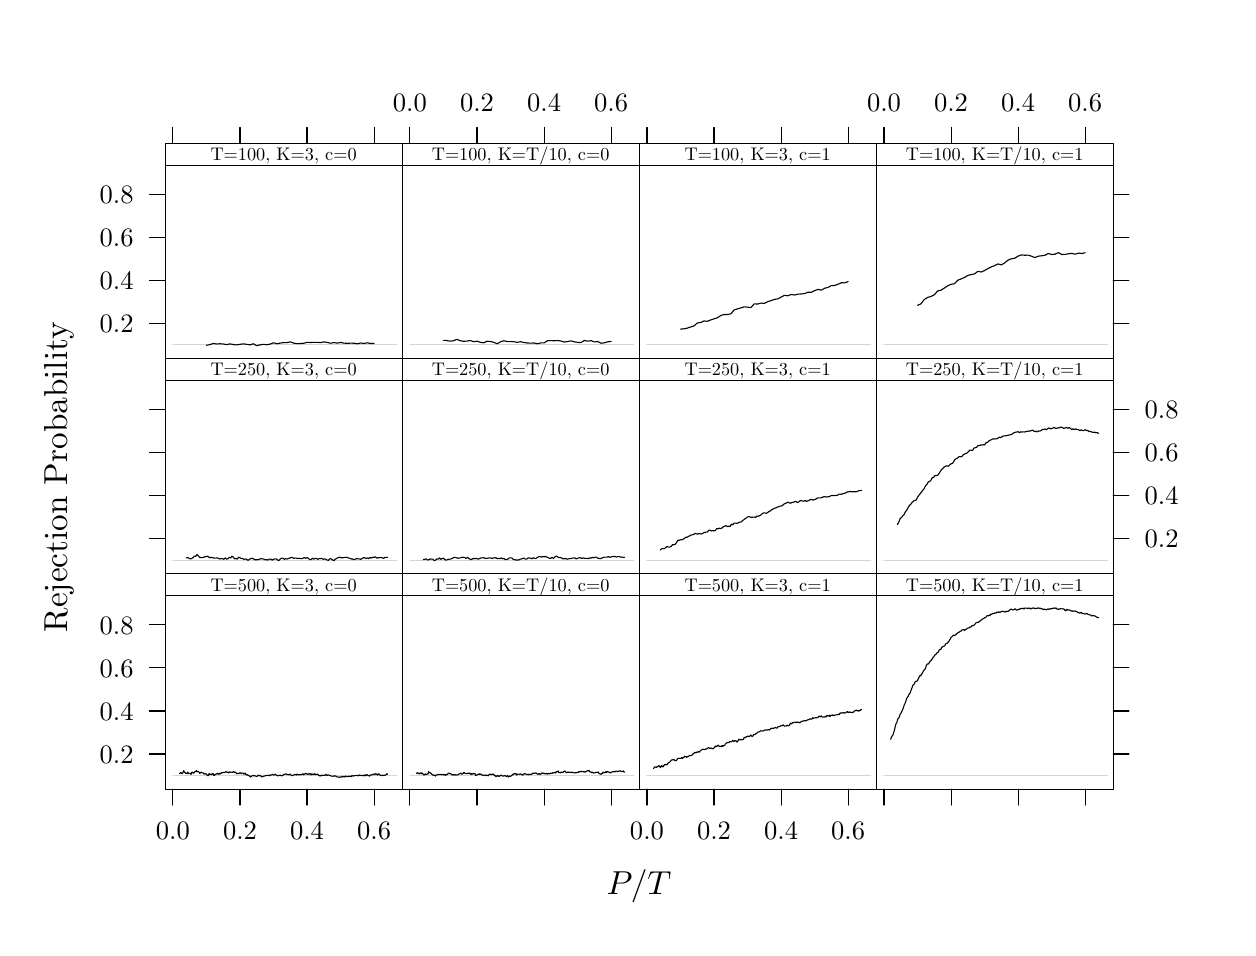
\begin{tikzpicture}[x=1pt,y=1pt]
\definecolor[named]{fillColor}{rgb}{1.00,1.00,1.00}
\path[use as bounding box,fill=fillColor,fill opacity=0.00] (0,0) rectangle (433.62,325.21);
\begin{scope}
\path[clip] (  0.00,  0.00) rectangle (433.62,325.21);

\path[] (  0.00,  0.00) rectangle (433.62,325.21);
\definecolor[named]{drawColor}{rgb}{0.00,0.00,0.00}

\node[text=drawColor,anchor=base,inner sep=0pt, outer sep=0pt, scale=  1.20] at (220.94, 12.05) {$P/T$};
\end{scope}
\begin{scope}
\path[clip] (  0.00,  0.00) rectangle (433.62,325.21);
\definecolor[named]{drawColor}{rgb}{0.00,0.00,0.00}

\node[text=drawColor,rotate= 90.00,anchor=base,inner sep=0pt, outer sep=0pt, scale=  1.20] at ( 14.29,162.76) {Rejection Probability};
\end{scope}
\begin{scope}
\path[clip] (  0.00,  0.00) rectangle (433.62,325.21);
\definecolor[named]{drawColor}{rgb}{0.00,0.00,0.00}

\path[draw=drawColor,line width= 0.4pt,line join=round,line cap=round] ( 49.65, 62.74) -- ( 43.95, 62.74);

\path[draw=drawColor,line width= 0.4pt,line join=round,line cap=round] ( 49.65, 78.30) -- ( 43.95, 78.30);

\path[draw=drawColor,line width= 0.4pt,line join=round,line cap=round] ( 49.65, 93.85) -- ( 43.95, 93.85);

\path[draw=drawColor,line width= 0.4pt,line join=round,line cap=round] ( 49.65,109.41) -- ( 43.95,109.41);

\node[text=drawColor,anchor=base east,inner sep=0pt, outer sep=0pt, scale=  0.96] at ( 38.26, 59.44) {0.2};

\node[text=drawColor,anchor=base east,inner sep=0pt, outer sep=0pt, scale=  0.96] at ( 38.26, 74.99) {0.4};

\node[text=drawColor,anchor=base east,inner sep=0pt, outer sep=0pt, scale=  0.96] at ( 38.26, 90.55) {0.6};

\node[text=drawColor,anchor=base east,inner sep=0pt, outer sep=0pt, scale=  0.96] at ( 38.26,106.10) {0.8};
\end{scope}
\begin{scope}
\path[clip] (  0.00,  0.00) rectangle (433.62,325.21);
\definecolor[named]{drawColor}{rgb}{0.00,0.00,0.00}

\path[draw=drawColor,line width= 0.4pt,line join=round,line cap=round] ( 52.48, 50.02) -- ( 52.48, 44.32);

\path[draw=drawColor,line width= 0.4pt,line join=round,line cap=round] ( 76.72, 50.02) -- ( 76.72, 44.32);

\path[draw=drawColor,line width= 0.4pt,line join=round,line cap=round] (100.95, 50.02) -- (100.95, 44.32);

\path[draw=drawColor,line width= 0.4pt,line join=round,line cap=round] (125.19, 50.02) -- (125.19, 44.32);

\node[text=drawColor,anchor=base,inner sep=0pt, outer sep=0pt, scale=  0.96] at ( 52.48, 32.02) {0.0};

\node[text=drawColor,anchor=base,inner sep=0pt, outer sep=0pt, scale=  0.96] at ( 76.72, 32.02) {0.2};

\node[text=drawColor,anchor=base,inner sep=0pt, outer sep=0pt, scale=  0.96] at (100.95, 32.02) {0.4};

\node[text=drawColor,anchor=base,inner sep=0pt, outer sep=0pt, scale=  0.96] at (125.19, 32.02) {0.6};
\end{scope}
\begin{scope}
\path[clip] ( 49.65, 50.02) rectangle (135.29,119.88);
\definecolor[named]{drawColor}{rgb}{0.83,0.83,0.83}

\path[draw=drawColor,line width= 0.4pt,line join=round,line cap=round] ( 52.48, 54.97) --
	(133.27, 54.97);
\definecolor[named]{drawColor}{rgb}{0.00,0.00,0.00}

\path[draw=drawColor,line width= 0.4pt,line join=round,line cap=round] ( 54.90, 55.71) --
	( 55.15, 55.98) --
	( 55.39, 56.13) --
	( 55.63, 55.67) --
	( 55.87, 55.74) --
	( 56.12, 56.06) --
	( 56.36, 56.76) --
	( 56.60, 56.25) --
	( 56.84, 56.09) --
	( 57.09, 55.82) --
	( 57.33, 55.78) --
	( 57.57, 55.59) --
	( 57.81, 56.21) --
	( 58.05, 55.90) --
	( 58.30, 55.71) --
	( 58.54, 55.78) --
	( 58.78, 55.67) --
	( 59.02, 55.39) --
	( 59.27, 56.09) --
	( 59.51, 56.21) --
	( 59.75, 55.86) --
	( 59.99, 55.82) --
	( 60.24, 56.13) --
	( 60.48, 56.41) --
	( 60.72, 56.41) --
	( 60.96, 56.76) --
	( 61.21, 56.29) --
	( 61.45, 56.41) --
	( 61.69, 56.44) --
	( 61.93, 56.21) --
	( 62.17, 55.78) --
	( 62.42, 55.94) --
	( 62.66, 56.17) --
	( 62.90, 56.09) --
	( 63.14, 55.94) --
	( 63.39, 55.90) --
	( 63.63, 55.71) --
	( 63.87, 55.43) --
	( 64.11, 55.63) --
	( 64.36, 55.59) --
	( 64.60, 55.55) --
	( 64.84, 55.12) --
	( 65.08, 54.89) --
	( 65.33, 55.01) --
	( 65.57, 55.71) --
	( 65.81, 55.39) --
	( 66.05, 55.47) --
	( 66.29, 55.24) --
	( 66.54, 55.39) --
	( 66.78, 55.74) --
	( 67.02, 55.63) --
	( 67.26, 55.01) --
	( 67.51, 55.01) --
	( 67.75, 55.36) --
	( 67.99, 55.47) --
	( 68.23, 55.47) --
	( 68.48, 55.82) --
	( 68.72, 55.67) --
	( 68.96, 55.43) --
	( 69.20, 55.47) --
	( 69.45, 55.82) --
	( 69.69, 55.59) --
	( 69.93, 55.90) --
	( 70.17, 56.02) --
	( 70.41, 55.94) --
	( 70.66, 56.02) --
	( 70.90, 56.17) --
	( 71.14, 55.94) --
	( 71.38, 56.17) --
	( 71.63, 56.37) --
	( 71.87, 56.29) --
	( 72.11, 56.09) --
	( 72.35, 56.25) --
	( 72.60, 55.90) --
	( 72.84, 56.25) --
	( 73.08, 56.25) --
	( 73.32, 56.09) --
	( 73.57, 56.21) --
	( 73.81, 56.17) --
	( 74.05, 56.06) --
	( 74.29, 56.37) --
	( 74.53, 56.29) --
	( 74.78, 56.09) --
	( 75.02, 56.17) --
	( 75.26, 56.06) --
	( 75.50, 55.63) --
	( 75.75, 55.67) --
	( 75.99, 55.78) --
	( 76.23, 55.63) --
	( 76.47, 55.74) --
	( 76.72, 55.98) --
	( 76.96, 55.94) --
	( 77.20, 55.59) --
	( 77.44, 55.82) --
	( 77.69, 55.86) --
	( 77.93, 55.78) --
	( 78.17, 55.43) --
	( 78.41, 55.78) --
	( 78.66, 55.78) --
	( 78.90, 55.28) --
	( 79.14, 55.16) --
	( 79.38, 55.28) --
	( 79.62, 55.08) --
	( 79.87, 55.01) --
	( 80.11, 54.85) --
	( 80.35, 54.62) --
	( 80.59, 54.42) --
	( 80.84, 54.77) --
	( 81.08, 54.85) --
	( 81.32, 54.93) --
	( 81.56, 54.85) --
	( 81.81, 55.01) --
	( 82.05, 54.85) --
	( 82.29, 54.85) --
	( 82.53, 54.69) --
	( 82.78, 54.66) --
	( 83.02, 54.77) --
	( 83.26, 55.08) --
	( 83.50, 55.08) --
	( 83.74, 54.85) --
	( 83.99, 55.01) --
	( 84.23, 54.85) --
	( 84.47, 54.50) --
	( 84.71, 54.50) --
	( 84.96, 54.54) --
	( 85.20, 54.77) --
	( 85.44, 54.73) --
	( 85.68, 54.77) --
	( 85.93, 55.04) --
	( 86.17, 54.89) --
	( 86.41, 55.04) --
	( 86.65, 55.01) --
	( 86.90, 55.16) --
	( 87.14, 54.97) --
	( 87.38, 54.89) --
	( 87.62, 55.12) --
	( 87.86, 55.16) --
	( 88.11, 55.16) --
	( 88.35, 55.36) --
	( 88.59, 55.36) --
	( 88.83, 55.12) --
	( 89.08, 55.20) --
	( 89.32, 55.28) --
	( 89.56, 55.47) --
	( 89.80, 55.12) --
	( 90.05, 55.01) --
	( 90.29, 54.89) --
	( 90.53, 54.85) --
	( 90.77, 55.01) --
	( 91.02, 55.04) --
	( 91.26, 55.08) --
	( 91.50, 55.01) --
	( 91.74, 54.81) --
	( 91.98, 54.93) --
	( 92.23, 55.08) --
	( 92.47, 55.24) --
	( 92.71, 55.39) --
	( 92.95, 55.47) --
	( 93.20, 55.59) --
	( 93.44, 55.43) --
	( 93.68, 55.47) --
	( 93.92, 55.32) --
	( 94.17, 55.32) --
	( 94.41, 55.20) --
	( 94.65, 55.43) --
	( 94.89, 55.43) --
	( 95.14, 55.12) --
	( 95.38, 55.04) --
	( 95.62, 54.89) --
	( 95.86, 55.04) --
	( 96.10, 55.16) --
	( 96.35, 55.28) --
	( 96.59, 55.36) --
	( 96.83, 55.28) --
	( 97.07, 55.12) --
	( 97.32, 55.43) --
	( 97.56, 55.39) --
	( 97.80, 55.20) --
	( 98.04, 55.24) --
	( 98.29, 55.24) --
	( 98.53, 55.28) --
	( 98.77, 55.32) --
	( 99.01, 55.28) --
	( 99.26, 55.55) --
	( 99.50, 55.55) --
	( 99.74, 55.20) --
	( 99.98, 55.47) --
	(100.22, 55.59) --
	(100.47, 55.82) --
	(100.71, 55.63) --
	(100.95, 55.43) --
	(101.19, 55.47) --
	(101.44, 55.63) --
	(101.68, 55.39) --
	(101.92, 55.67) --
	(102.16, 55.55) --
	(102.41, 55.16) --
	(102.65, 55.59) --
	(102.89, 55.43) --
	(103.13, 55.28) --
	(103.38, 55.51) --
	(103.62, 55.63) --
	(103.86, 55.28) --
	(104.10, 55.47) --
	(104.34, 55.28) --
	(104.59, 55.51) --
	(104.83, 55.28) --
	(105.07, 55.20) --
	(105.31, 54.93) --
	(105.56, 54.81) --
	(105.80, 55.04) --
	(106.04, 54.85) --
	(106.28, 55.04) --
	(106.53, 55.08) --
	(106.77, 55.12) --
	(107.01, 55.01) --
	(107.25, 55.01) --
	(107.50, 55.20) --
	(107.74, 55.43) --
	(107.98, 55.01) --
	(108.22, 54.97) --
	(108.46, 55.20) --
	(108.71, 55.20) --
	(108.95, 55.08) --
	(109.19, 55.01) --
	(109.43, 54.89) --
	(109.68, 54.77) --
	(109.92, 54.77) --
	(110.16, 54.77) --
	(110.40, 54.66) --
	(110.65, 54.85) --
	(110.89, 54.81) --
	(111.13, 54.81) --
	(111.37, 54.81) --
	(111.62, 54.50) --
	(111.86, 54.46) --
	(112.10, 54.46) --
	(112.34, 54.38) --
	(112.58, 54.31) --
	(112.83, 54.46) --
	(113.07, 54.38) --
	(113.31, 54.54) --
	(113.55, 54.38) --
	(113.80, 54.73) --
	(114.04, 54.58) --
	(114.28, 54.54) --
	(114.52, 54.42) --
	(114.77, 54.81) --
	(115.01, 54.66) --
	(115.25, 54.62) --
	(115.49, 54.66) --
	(115.74, 54.54) --
	(115.98, 54.66) --
	(116.22, 54.73) --
	(116.46, 54.73) --
	(116.70, 54.66) --
	(116.95, 54.58) --
	(117.19, 54.97) --
	(117.43, 54.89) --
	(117.67, 54.73) --
	(117.92, 54.89) --
	(118.16, 54.93) --
	(118.40, 54.93) --
	(118.64, 55.01) --
	(118.89, 55.01) --
	(119.13, 55.01) --
	(119.37, 54.85) --
	(119.61, 54.97) --
	(119.86, 55.20) --
	(120.10, 54.93) --
	(120.34, 55.04) --
	(120.58, 55.01) --
	(120.83, 55.01) --
	(121.07, 54.93) --
	(121.31, 55.08) --
	(121.55, 54.85) --
	(121.79, 55.24) --
	(122.04, 55.12) --
	(122.28, 54.85) --
	(122.52, 55.24) --
	(122.76, 55.28) --
	(123.01, 55.01) --
	(123.25, 55.01) --
	(123.49, 54.73) --
	(123.73, 55.04) --
	(123.98, 55.24) --
	(124.22, 55.12) --
	(124.46, 55.24) --
	(124.70, 55.32) --
	(124.95, 55.51) --
	(125.19, 55.47) --
	(125.43, 55.24) --
	(125.67, 55.63) --
	(125.91, 55.55) --
	(126.16, 55.43) --
	(126.40, 55.12) --
	(126.64, 55.39) --
	(126.88, 55.63) --
	(127.13, 55.39) --
	(127.37, 55.04) --
	(127.61, 55.08) --
	(127.85, 54.97) --
	(128.10, 54.93) --
	(128.34, 55.08) --
	(128.58, 55.01) --
	(128.82, 55.04) --
	(129.07, 55.08) --
	(129.31, 55.16) --
	(129.55, 55.36) --
	(129.79, 55.63) --
	(130.03, 55.39);
\end{scope}
\begin{scope}
\path[clip] (  0.00,  0.00) rectangle (433.62,325.21);
\definecolor[named]{drawColor}{rgb}{0.00,0.00,0.00}

\path[draw=drawColor,line width= 0.4pt,line join=round,line cap=round] ( 49.65, 50.02) rectangle (135.29,119.88);
\end{scope}
\begin{scope}
\path[clip] ( 49.65,119.88) rectangle (135.29,127.83);

\path[] ( 49.65,119.88) rectangle (135.29,127.83);
\definecolor[named]{drawColor}{rgb}{0.00,0.00,0.00}

\node[text=drawColor,anchor=base west,inner sep=0pt, outer sep=0pt, scale=  0.66] at ( 66.08,121.58) {T=500, K=3, c=0};
\end{scope}
\begin{scope}
\path[clip] (  0.00,  0.00) rectangle (433.62,325.21);
\definecolor[named]{drawColor}{rgb}{0.00,0.00,0.00}

\path[draw=drawColor,line width= 0.4pt,line join=round,line cap=round] ( 49.65,119.88) rectangle (135.29,127.83);
\end{scope}
\begin{scope}
\path[clip] (  0.00,  0.00) rectangle (433.62,325.21);
\definecolor[named]{drawColor}{rgb}{0.00,0.00,0.00}

\path[draw=drawColor,line width= 0.4pt,line join=round,line cap=round] (138.13, 50.02) -- (138.13, 44.32);

\path[draw=drawColor,line width= 0.4pt,line join=round,line cap=round] (162.36, 50.02) -- (162.36, 44.32);

\path[draw=drawColor,line width= 0.4pt,line join=round,line cap=round] (186.60, 50.02) -- (186.60, 44.32);

\path[draw=drawColor,line width= 0.4pt,line join=round,line cap=round] (210.84, 50.02) -- (210.84, 44.32);
\end{scope}
\begin{scope}
\path[clip] (135.29, 50.02) rectangle (220.94,119.88);
\definecolor[named]{drawColor}{rgb}{0.83,0.83,0.83}

\path[draw=drawColor,line width= 0.4pt,line join=round,line cap=round] (138.13, 54.97) --
	(218.91, 54.97);
\definecolor[named]{drawColor}{rgb}{0.00,0.00,0.00}

\path[draw=drawColor,line width= 0.4pt,line join=round,line cap=round] (140.55, 55.67) --
	(140.80, 56.02) --
	(141.04, 55.78) --
	(141.28, 55.82) --
	(141.52, 55.55) --
	(141.76, 55.82) --
	(142.01, 55.94) --
	(142.25, 55.59) --
	(142.49, 55.90) --
	(142.73, 55.71) --
	(142.98, 55.32) --
	(143.22, 55.16) --
	(143.46, 55.24) --
	(143.70, 55.59) --
	(143.95, 55.36) --
	(144.19, 55.39) --
	(144.43, 55.51) --
	(144.67, 55.47) --
	(144.92, 56.37) --
	(145.16, 56.02) --
	(145.40, 55.98) --
	(145.64, 55.78) --
	(145.88, 55.67) --
	(146.13, 55.32) --
	(146.37, 55.28) --
	(146.61, 55.01) --
	(146.85, 55.04) --
	(147.10, 55.12) --
	(147.34, 54.77) --
	(147.58, 55.12) --
	(147.82, 55.12) --
	(148.07, 55.36) --
	(148.31, 55.28) --
	(148.55, 55.36) --
	(148.79, 55.28) --
	(149.04, 55.36) --
	(149.28, 55.28) --
	(149.52, 55.36) --
	(149.76, 55.24) --
	(150.00, 55.39) --
	(150.25, 55.24) --
	(150.49, 55.28) --
	(150.73, 55.36) --
	(150.97, 55.04) --
	(151.22, 55.28) --
	(151.46, 55.43) --
	(151.70, 55.28) --
	(151.94, 55.78) --
	(152.19, 55.86) --
	(152.43, 55.78) --
	(152.67, 55.59) --
	(152.91, 55.63) --
	(153.16, 55.32) --
	(153.40, 55.36) --
	(153.64, 55.12) --
	(153.88, 55.28) --
	(154.12, 55.16) --
	(154.37, 55.36) --
	(154.61, 55.16) --
	(154.85, 55.20) --
	(155.09, 55.16) --
	(155.34, 55.20) --
	(155.58, 55.28) --
	(155.82, 55.51) --
	(156.06, 55.55) --
	(156.31, 55.71) --
	(156.55, 55.86) --
	(156.79, 55.47) --
	(157.03, 55.47) --
	(157.28, 55.63) --
	(157.52, 56.09) --
	(157.76, 56.09) --
	(158.00, 55.74) --
	(158.24, 55.74) --
	(158.49, 55.67) --
	(158.73, 55.74) --
	(158.97, 55.71) --
	(159.21, 55.90) --
	(159.46, 55.71) --
	(159.70, 55.86) --
	(159.94, 55.59) --
	(160.18, 55.36) --
	(160.43, 55.67) --
	(160.67, 55.47) --
	(160.91, 55.67) --
	(161.15, 55.55) --
	(161.40, 55.67) --
	(161.64, 55.63) --
	(161.88, 55.04) --
	(162.12, 55.04) --
	(162.36, 55.20) --
	(162.61, 55.36) --
	(162.85, 55.43) --
	(163.09, 55.36) --
	(163.33, 55.59) --
	(163.58, 55.39) --
	(163.82, 55.47) --
	(164.06, 55.28) --
	(164.30, 55.08) --
	(164.55, 55.01) --
	(164.79, 55.12) --
	(165.03, 55.12) --
	(165.27, 54.97) --
	(165.52, 55.12) --
	(165.76, 55.16) --
	(166.00, 54.97) --
	(166.24, 55.04) --
	(166.48, 54.89) --
	(166.73, 55.32) --
	(166.97, 55.43) --
	(167.21, 55.51) --
	(167.45, 55.24) --
	(167.70, 55.39) --
	(167.94, 55.32) --
	(168.18, 55.55) --
	(168.42, 55.39) --
	(168.67, 54.97) --
	(168.91, 54.97) --
	(169.15, 54.62) --
	(169.39, 54.62) --
	(169.64, 54.97) --
	(169.88, 54.97) --
	(170.12, 54.66) --
	(170.36, 54.69) --
	(170.60, 54.89) --
	(170.85, 54.89) --
	(171.09, 55.16) --
	(171.33, 55.01) --
	(171.57, 54.81) --
	(171.82, 54.73) --
	(172.06, 54.85) --
	(172.30, 54.93) --
	(172.54, 54.85) --
	(172.79, 54.77) --
	(173.03, 54.66) --
	(173.27, 54.93) --
	(173.51, 54.66) --
	(173.76, 54.42) --
	(174.00, 54.81) --
	(174.24, 54.73) --
	(174.48, 54.69) --
	(174.73, 54.85) --
	(174.97, 55.01) --
	(175.21, 55.43) --
	(175.45, 55.24) --
	(175.69, 55.59) --
	(175.94, 55.71) --
	(176.18, 55.55) --
	(176.42, 55.71) --
	(176.66, 55.12) --
	(176.91, 55.39) --
	(177.15, 55.47) --
	(177.39, 55.47) --
	(177.63, 55.43) --
	(177.88, 55.47) --
	(178.12, 55.59) --
	(178.36, 55.39) --
	(178.60, 55.32) --
	(178.85, 55.12) --
	(179.09, 55.28) --
	(179.33, 55.59) --
	(179.57, 55.67) --
	(179.81, 55.55) --
	(180.06, 55.47) --
	(180.30, 55.36) --
	(180.54, 55.28) --
	(180.78, 55.43) --
	(181.03, 55.24) --
	(181.27, 55.36) --
	(181.51, 55.47) --
	(181.75, 55.32) --
	(182.00, 55.39) --
	(182.24, 55.51) --
	(182.48, 55.82) --
	(182.72, 55.71) --
	(182.97, 55.86) --
	(183.21, 55.74) --
	(183.45, 55.86) --
	(183.69, 55.90) --
	(183.93, 55.67) --
	(184.18, 55.51) --
	(184.42, 55.39) --
	(184.66, 55.63) --
	(184.90, 55.63) --
	(185.15, 55.39) --
	(185.39, 55.39) --
	(185.63, 55.78) --
	(185.87, 55.94) --
	(186.12, 55.67) --
	(186.36, 55.86) --
	(186.60, 55.59) --
	(186.84, 55.74) --
	(187.09, 55.63) --
	(187.33, 55.59) --
	(187.57, 55.71) --
	(187.81, 55.47) --
	(188.05, 55.74) --
	(188.30, 55.71) --
	(188.54, 55.59) --
	(188.78, 55.63) --
	(189.02, 55.82) --
	(189.27, 55.82) --
	(189.51, 55.74) --
	(189.75, 55.98) --
	(189.99, 55.94) --
	(190.24, 55.98) --
	(190.48, 56.09) --
	(190.72, 55.86) --
	(190.96, 56.33) --
	(191.21, 56.33) --
	(191.45, 56.44) --
	(191.69, 56.60) --
	(191.93, 55.98) --
	(192.17, 56.09) --
	(192.42, 55.94) --
	(192.66, 56.13) --
	(192.90, 56.17) --
	(193.14, 56.06) --
	(193.39, 56.09) --
	(193.63, 56.37) --
	(193.87, 56.41) --
	(194.11, 56.64) --
	(194.36, 56.33) --
	(194.60, 55.98) --
	(194.84, 56.06) --
	(195.08, 56.21) --
	(195.33, 56.09) --
	(195.57, 56.25) --
	(195.81, 56.17) --
	(196.05, 56.09) --
	(196.29, 55.98) --
	(196.54, 56.25) --
	(196.78, 56.09) --
	(197.02, 56.13) --
	(197.26, 56.09) --
	(197.51, 55.86) --
	(197.75, 55.94) --
	(197.99, 55.98) --
	(198.23, 55.98) --
	(198.48, 56.13) --
	(198.72, 56.06) --
	(198.96, 56.06) --
	(199.20, 56.41) --
	(199.45, 56.33) --
	(199.69, 56.48) --
	(199.93, 56.33) --
	(200.17, 56.44) --
	(200.41, 56.41) --
	(200.66, 56.41) --
	(200.90, 56.25) --
	(201.14, 56.37) --
	(201.38, 56.13) --
	(201.63, 56.37) --
	(201.87, 56.44) --
	(202.11, 56.64) --
	(202.35, 56.76) --
	(202.60, 56.68) --
	(202.84, 56.83) --
	(203.08, 56.33) --
	(203.32, 56.29) --
	(203.57, 56.25) --
	(203.81, 55.98) --
	(204.05, 56.21) --
	(204.29, 56.02) --
	(204.53, 55.86) --
	(204.78, 55.94) --
	(205.02, 55.98) --
	(205.26, 56.13) --
	(205.50, 56.06) --
	(205.75, 56.09) --
	(205.99, 56.17) --
	(206.23, 56.25) --
	(206.47, 55.59) --
	(206.72, 55.59) --
	(206.96, 55.55) --
	(207.20, 55.39) --
	(207.44, 55.74) --
	(207.69, 55.67) --
	(207.93, 56.25) --
	(208.17, 56.02) --
	(208.41, 56.06) --
	(208.65, 55.90) --
	(208.90, 56.37) --
	(209.14, 56.09) --
	(209.38, 56.44) --
	(209.62, 56.29) --
	(209.87, 56.17) --
	(210.11, 56.29) --
	(210.35, 55.98) --
	(210.59, 56.02) --
	(210.84, 55.94) --
	(211.08, 56.25) --
	(211.32, 56.37) --
	(211.56, 56.41) --
	(211.81, 56.29) --
	(212.05, 56.37) --
	(212.29, 56.33) --
	(212.53, 56.56) --
	(212.77, 56.56) --
	(213.02, 56.41) --
	(213.26, 56.41) --
	(213.50, 56.56) --
	(213.74, 56.68) --
	(213.99, 56.52) --
	(214.23, 56.64) --
	(214.47, 56.44) --
	(214.71, 56.41) --
	(214.96, 56.48) --
	(215.20, 56.64) --
	(215.44, 56.25) --
	(215.68, 56.25);
\end{scope}
\begin{scope}
\path[clip] (  0.00,  0.00) rectangle (433.62,325.21);
\definecolor[named]{drawColor}{rgb}{0.00,0.00,0.00}

\path[draw=drawColor,line width= 0.4pt,line join=round,line cap=round] (135.29, 50.02) rectangle (220.94,119.88);
\end{scope}
\begin{scope}
\path[clip] (135.29,119.88) rectangle (220.94,127.83);

\path[] (135.29,119.88) rectangle (220.94,127.83);
\definecolor[named]{drawColor}{rgb}{0.00,0.00,0.00}

\node[text=drawColor,anchor=base west,inner sep=0pt, outer sep=0pt, scale=  0.66] at (146.04,121.58) {T=500, K=T/10, c=0};
\end{scope}
\begin{scope}
\path[clip] (  0.00,  0.00) rectangle (433.62,325.21);
\definecolor[named]{drawColor}{rgb}{0.00,0.00,0.00}

\path[draw=drawColor,line width= 0.4pt,line join=round,line cap=round] (135.29,119.88) rectangle (220.94,127.83);
\end{scope}
\begin{scope}
\path[clip] (  0.00,  0.00) rectangle (433.62,325.21);
\definecolor[named]{drawColor}{rgb}{0.00,0.00,0.00}

\path[draw=drawColor,line width= 0.4pt,line join=round,line cap=round] (223.78, 50.02) -- (223.78, 44.32);

\path[draw=drawColor,line width= 0.4pt,line join=round,line cap=round] (248.01, 50.02) -- (248.01, 44.32);

\path[draw=drawColor,line width= 0.4pt,line join=round,line cap=round] (272.25, 50.02) -- (272.25, 44.32);

\path[draw=drawColor,line width= 0.4pt,line join=round,line cap=round] (296.48, 50.02) -- (296.48, 44.32);

\node[text=drawColor,anchor=base,inner sep=0pt, outer sep=0pt, scale=  0.96] at (223.78, 32.02) {0.0};

\node[text=drawColor,anchor=base,inner sep=0pt, outer sep=0pt, scale=  0.96] at (248.01, 32.02) {0.2};

\node[text=drawColor,anchor=base,inner sep=0pt, outer sep=0pt, scale=  0.96] at (272.25, 32.02) {0.4};

\node[text=drawColor,anchor=base,inner sep=0pt, outer sep=0pt, scale=  0.96] at (296.48, 32.02) {0.6};
\end{scope}
\begin{scope}
\path[clip] (220.94, 50.02) rectangle (306.59,119.88);
\definecolor[named]{drawColor}{rgb}{0.83,0.83,0.83}

\path[draw=drawColor,line width= 0.4pt,line join=round,line cap=round] (223.78, 54.97) --
	(304.56, 54.97);
\definecolor[named]{drawColor}{rgb}{0.00,0.00,0.00}

\path[draw=drawColor,line width= 0.4pt,line join=round,line cap=round] (226.20, 57.49) --
	(226.44, 57.92) --
	(226.69, 58.08) --
	(226.93, 58.04) --
	(227.17, 57.92) --
	(227.41, 58.19) --
	(227.66, 58.04) --
	(227.90, 58.43) --
	(228.14, 58.54) --
	(228.38, 58.31) --
	(228.62, 57.81) --
	(228.87, 58.19) --
	(229.11, 58.58) --
	(229.35, 58.23) --
	(229.59, 58.08) --
	(229.84, 58.51) --
	(230.08, 58.93) --
	(230.32, 58.86) --
	(230.56, 59.05) --
	(230.81, 58.78) --
	(231.05, 58.89) --
	(231.29, 59.36) --
	(231.53, 59.52) --
	(231.78, 59.75) --
	(232.02, 59.79) --
	(232.26, 60.10) --
	(232.50, 60.53) --
	(232.75, 60.61) --
	(232.99, 60.68) --
	(233.23, 60.57) --
	(233.47, 60.80) --
	(233.71, 60.53) --
	(233.96, 60.37) --
	(234.20, 60.37) --
	(234.44, 60.45) --
	(234.68, 60.80) --
	(234.93, 61.15) --
	(235.17, 61.19) --
	(235.41, 61.15) --
	(235.65, 61.23) --
	(235.90, 61.19) --
	(236.14, 61.19) --
	(236.38, 61.46) --
	(236.62, 61.19) --
	(236.87, 61.42) --
	(237.11, 61.50) --
	(237.35, 61.97) --
	(237.59, 61.85) --
	(237.83, 61.81) --
	(238.08, 61.54) --
	(238.32, 61.77) --
	(238.56, 61.73) --
	(238.80, 61.93) --
	(239.05, 62.08) --
	(239.29, 62.20) --
	(239.53, 62.16) --
	(239.77, 62.24) --
	(240.02, 62.32) --
	(240.26, 62.47) --
	(240.50, 62.94) --
	(240.74, 62.86) --
	(240.99, 63.37) --
	(241.23, 63.25) --
	(241.47, 63.17) --
	(241.71, 63.37) --
	(241.95, 63.48) --
	(242.20, 63.37) --
	(242.44, 63.64) --
	(242.68, 63.41) --
	(242.92, 63.79) --
	(243.17, 64.03) --
	(243.41, 64.14) --
	(243.65, 64.34) --
	(243.89, 64.42) --
	(244.14, 64.49) --
	(244.38, 64.38) --
	(244.62, 64.34) --
	(244.86, 64.46) --
	(245.11, 64.61) --
	(245.35, 64.53) --
	(245.59, 64.84) --
	(245.83, 64.92) --
	(246.07, 65.08) --
	(246.32, 64.84) --
	(246.56, 64.77) --
	(246.80, 64.92) --
	(247.04, 64.88) --
	(247.29, 64.69) --
	(247.53, 64.65) --
	(247.77, 64.69) --
	(248.01, 65.00) --
	(248.26, 65.23) --
	(248.50, 65.66) --
	(248.74, 65.39) --
	(248.98, 65.47) --
	(249.23, 65.70) --
	(249.47, 65.97) --
	(249.71, 65.66) --
	(249.95, 65.50) --
	(250.19, 65.58) --
	(250.44, 65.47) --
	(250.68, 65.35) --
	(250.92, 65.82) --
	(251.16, 65.50) --
	(251.41, 65.82) --
	(251.65, 65.82) --
	(251.89, 65.93) --
	(252.13, 66.40) --
	(252.38, 66.67) --
	(252.62, 66.79) --
	(252.86, 66.83) --
	(253.10, 66.94) --
	(253.35, 66.90) --
	(253.59, 67.10) --
	(253.83, 67.29) --
	(254.07, 67.14) --
	(254.31, 67.18) --
	(254.56, 67.37) --
	(254.80, 67.68) --
	(255.04, 67.37) --
	(255.28, 67.33) --
	(255.53, 67.57) --
	(255.77, 67.53) --
	(256.01, 67.45) --
	(256.25, 67.06) --
	(256.50, 67.22) --
	(256.74, 67.64) --
	(256.98, 68.11) --
	(257.22, 67.88) --
	(257.47, 67.88) --
	(257.71, 68.07) --
	(257.95, 67.88) --
	(258.19, 67.95) --
	(258.43, 67.92) --
	(258.68, 68.07) --
	(258.92, 68.73) --
	(259.16, 68.77) --
	(259.40, 68.65) --
	(259.65, 69.00) --
	(259.89, 69.04) --
	(260.13, 69.20) --
	(260.37, 69.16) --
	(260.62, 69.12) --
	(260.86, 69.16) --
	(261.10, 69.32) --
	(261.34, 69.63) --
	(261.59, 69.20) --
	(261.83, 69.16) --
	(262.07, 69.24) --
	(262.31, 69.82) --
	(262.55, 69.78) --
	(262.80, 69.82) --
	(263.04, 69.98) --
	(263.28, 70.17) --
	(263.52, 70.37) --
	(263.77, 70.52) --
	(264.01, 70.72) --
	(264.25, 70.75) --
	(264.49, 70.83) --
	(264.74, 71.07) --
	(264.98, 71.14) --
	(265.22, 71.10) --
	(265.46, 71.03) --
	(265.71, 71.10) --
	(265.95, 71.14) --
	(266.19, 71.26) --
	(266.43, 71.49) --
	(266.67, 71.45) --
	(266.92, 71.34) --
	(267.16, 71.45) --
	(267.40, 71.38) --
	(267.64, 71.57) --
	(267.89, 71.53) --
	(268.13, 71.42) --
	(268.37, 71.80) --
	(268.61, 71.96) --
	(268.86, 72.08) --
	(269.10, 72.04) --
	(269.34, 72.00) --
	(269.58, 72.00) --
	(269.83, 72.19) --
	(270.07, 72.35) --
	(270.31, 72.23) --
	(270.55, 72.15) --
	(270.79, 72.12) --
	(271.04, 72.47) --
	(271.28, 72.66) --
	(271.52, 72.66) --
	(271.76, 72.62) --
	(272.01, 72.89) --
	(272.25, 72.97) --
	(272.49, 73.05) --
	(272.73, 72.93) --
	(272.98, 73.28) --
	(273.22, 73.09) --
	(273.46, 72.78) --
	(273.70, 72.85) --
	(273.95, 72.82) --
	(274.19, 73.01) --
	(274.43, 73.17) --
	(274.67, 72.97) --
	(274.92, 72.89) --
	(275.16, 73.05) --
	(275.40, 73.40) --
	(275.64, 73.90) --
	(275.88, 73.67) --
	(276.13, 73.75) --
	(276.37, 74.10) --
	(276.61, 73.98) --
	(276.85, 74.14) --
	(277.10, 74.29) --
	(277.34, 74.25) --
	(277.58, 74.10) --
	(277.82, 74.22) --
	(278.07, 74.33) --
	(278.31, 74.18) --
	(278.55, 74.06) --
	(278.79, 74.25) --
	(279.04, 74.02) --
	(279.28, 74.29) --
	(279.52, 74.45) --
	(279.76, 74.57) --
	(280.00, 74.64) --
	(280.25, 74.68) --
	(280.49, 74.76) --
	(280.73, 74.72) --
	(280.97, 74.80) --
	(281.22, 74.72) --
	(281.46, 74.88) --
	(281.70, 75.03) --
	(281.94, 75.11) --
	(282.19, 75.15) --
	(282.43, 75.27) --
	(282.67, 75.46) --
	(282.91, 75.34) --
	(283.16, 75.42) --
	(283.40, 75.34) --
	(283.64, 75.85) --
	(283.88, 75.65) --
	(284.12, 75.73) --
	(284.37, 75.81) --
	(284.61, 75.85) --
	(284.85, 75.81) --
	(285.09, 75.77) --
	(285.34, 75.97) --
	(285.58, 76.04) --
	(285.82, 76.28) --
	(286.06, 76.43) --
	(286.31, 76.28) --
	(286.55, 76.16) --
	(286.79, 76.55) --
	(287.03, 76.16) --
	(287.28, 76.04) --
	(287.52, 76.12) --
	(287.76, 76.08) --
	(288.00, 76.08) --
	(288.24, 76.35) --
	(288.49, 76.16) --
	(288.73, 76.63) --
	(288.97, 76.67) --
	(289.21, 76.43) --
	(289.46, 76.51) --
	(289.70, 76.78) --
	(289.94, 76.32) --
	(290.18, 76.63) --
	(290.43, 76.78) --
	(290.67, 76.63) --
	(290.91, 76.90) --
	(291.15, 76.63) --
	(291.40, 76.59) --
	(291.64, 76.78) --
	(291.88, 76.90) --
	(292.12, 76.90) --
	(292.36, 76.86) --
	(292.61, 76.98) --
	(292.85, 77.13) --
	(293.09, 76.98) --
	(293.33, 77.05) --
	(293.58, 77.60) --
	(293.82, 77.56) --
	(294.06, 77.56) --
	(294.30, 77.56) --
	(294.55, 77.64) --
	(294.79, 77.75) --
	(295.03, 77.48) --
	(295.27, 77.60) --
	(295.52, 77.64) --
	(295.76, 77.79) --
	(296.00, 77.99) --
	(296.24, 78.10) --
	(296.48, 77.72) --
	(296.73, 77.83) --
	(296.97, 77.95) --
	(297.21, 77.72) --
	(297.45, 77.95) --
	(297.70, 77.72) --
	(297.94, 77.72) --
	(298.18, 77.91) --
	(298.42, 77.83) --
	(298.67, 78.26) --
	(298.91, 78.34) --
	(299.15, 78.42) --
	(299.39, 78.61) --
	(299.64, 78.42) --
	(299.88, 78.30) --
	(300.12, 78.45) --
	(300.36, 78.22) --
	(300.60, 78.53) --
	(300.85, 78.45) --
	(301.09, 78.80) --
	(301.33, 78.84);
\end{scope}
\begin{scope}
\path[clip] (  0.00,  0.00) rectangle (433.62,325.21);
\definecolor[named]{drawColor}{rgb}{0.00,0.00,0.00}

\path[draw=drawColor,line width= 0.4pt,line join=round,line cap=round] (220.94, 50.02) rectangle (306.59,119.88);
\end{scope}
\begin{scope}
\path[clip] (220.94,119.88) rectangle (306.59,127.83);

\path[] (220.94,119.88) rectangle (306.59,127.83);
\definecolor[named]{drawColor}{rgb}{0.00,0.00,0.00}

\node[text=drawColor,anchor=base west,inner sep=0pt, outer sep=0pt, scale=  0.66] at (237.37,121.58) {T=500, K=3, c=1};
\end{scope}
\begin{scope}
\path[clip] (  0.00,  0.00) rectangle (433.62,325.21);
\definecolor[named]{drawColor}{rgb}{0.00,0.00,0.00}

\path[draw=drawColor,line width= 0.4pt,line join=round,line cap=round] (220.94,119.88) rectangle (306.59,127.83);
\end{scope}
\begin{scope}
\path[clip] (  0.00,  0.00) rectangle (433.62,325.21);
\definecolor[named]{drawColor}{rgb}{0.00,0.00,0.00}

\path[draw=drawColor,line width= 0.4pt,line join=round,line cap=round] (309.43, 50.02) -- (309.43, 44.32);

\path[draw=drawColor,line width= 0.4pt,line join=round,line cap=round] (333.66, 50.02) -- (333.66, 44.32);

\path[draw=drawColor,line width= 0.4pt,line join=round,line cap=round] (357.90, 50.02) -- (357.90, 44.32);

\path[draw=drawColor,line width= 0.4pt,line join=round,line cap=round] (382.13, 50.02) -- (382.13, 44.32);

\path[draw=drawColor,line width= 0.4pt,line join=round,line cap=round] (392.24, 62.74) -- (397.93, 62.74);

\path[draw=drawColor,line width= 0.4pt,line join=round,line cap=round] (392.24, 78.30) -- (397.93, 78.30);

\path[draw=drawColor,line width= 0.4pt,line join=round,line cap=round] (392.24, 93.85) -- (397.93, 93.85);

\path[draw=drawColor,line width= 0.4pt,line join=round,line cap=round] (392.24,109.41) -- (397.93,109.41);
\end{scope}
\begin{scope}
\path[clip] (306.59, 50.02) rectangle (392.24,119.88);
\definecolor[named]{drawColor}{rgb}{0.83,0.83,0.83}

\path[draw=drawColor,line width= 0.4pt,line join=round,line cap=round] (309.43, 54.97) --
	(390.21, 54.97);
\definecolor[named]{drawColor}{rgb}{0.00,0.00,0.00}

\path[draw=drawColor,line width= 0.4pt,line join=round,line cap=round] (311.85, 68.07) --
	(312.09, 68.74) --
	(312.33, 69.21) --
	(312.58, 69.47) --
	(312.82, 70.16) --
	(313.06, 70.94) --
	(313.30, 71.70) --
	(313.55, 73.01) --
	(313.79, 73.73) --
	(314.03, 73.98) --
	(314.27, 74.89) --
	(314.52, 75.60) --
	(314.76, 75.82) --
	(315.00, 76.14) --
	(315.24, 77.07) --
	(315.49, 77.37) --
	(315.73, 77.85) --
	(315.97, 78.32) --
	(316.21, 78.95) --
	(316.45, 79.47) --
	(316.70, 80.38) --
	(316.94, 80.83) --
	(317.18, 81.35) --
	(317.42, 82.15) --
	(317.67, 82.95) --
	(317.91, 83.25) --
	(318.15, 83.57) --
	(318.39, 84.18) --
	(318.64, 84.56) --
	(318.88, 84.78) --
	(319.12, 85.54) --
	(319.36, 86.16) --
	(319.61, 86.85) --
	(319.85, 87.57) --
	(320.09, 87.72) --
	(320.33, 87.98) --
	(320.57, 88.60) --
	(320.82, 88.93) --
	(321.06, 89.01) --
	(321.30, 89.12) --
	(321.54, 89.25) --
	(321.79, 89.88) --
	(322.03, 90.37) --
	(322.27, 90.80) --
	(322.51, 91.15) --
	(322.76, 91.02) --
	(323.00, 91.67) --
	(323.24, 91.82) --
	(323.48, 92.36) --
	(323.73, 92.77) --
	(323.97, 93.20) --
	(324.21, 93.29) --
	(324.45, 93.83) --
	(324.69, 94.65) --
	(324.94, 95.12) --
	(325.18, 95.32) --
	(325.42, 95.27) --
	(325.66, 95.55) --
	(325.91, 96.01) --
	(326.15, 96.29) --
	(326.39, 96.40) --
	(326.63, 97.04) --
	(326.88, 97.00) --
	(327.12, 97.69) --
	(327.36, 97.74) --
	(327.60, 98.21) --
	(327.85, 98.58) --
	(328.09, 98.66) --
	(328.33, 98.94) --
	(328.57, 99.35) --
	(328.82, 99.35) --
	(329.06, 99.61) --
	(329.30,100.24) --
	(329.54,100.41) --
	(329.78,100.59) --
	(330.03,100.61) --
	(330.27,101.23) --
	(330.51,101.49) --
	(330.75,101.51) --
	(331.00,101.64) --
	(331.24,101.77) --
	(331.48,102.08) --
	(331.72,102.55) --
	(331.97,102.68) --
	(332.21,102.74) --
	(332.45,102.96) --
	(332.69,103.28) --
	(332.94,103.54) --
	(333.18,104.00) --
	(333.42,104.36) --
	(333.66,104.93) --
	(333.90,105.06) --
	(334.15,105.42) --
	(334.39,105.44) --
	(334.63,105.70) --
	(334.87,105.53) --
	(335.12,105.70) --
	(335.36,105.83) --
	(335.60,106.09) --
	(335.84,106.37) --
	(336.09,106.50) --
	(336.33,106.70) --
	(336.57,106.76) --
	(336.81,106.93) --
	(337.06,107.15) --
	(337.30,107.15) --
	(337.54,107.54) --
	(337.78,107.58) --
	(338.02,107.65) --
	(338.27,107.73) --
	(338.51,107.39) --
	(338.75,107.62) --
	(338.99,107.75) --
	(339.24,107.91) --
	(339.48,108.10) --
	(339.72,108.21) --
	(339.96,108.32) --
	(340.21,108.32) --
	(340.45,108.62) --
	(340.69,108.60) --
	(340.93,108.75) --
	(341.18,109.09) --
	(341.42,109.03) --
	(341.66,109.16) --
	(341.90,109.27) --
	(342.14,109.52) --
	(342.39,109.74) --
	(342.63,110.13) --
	(342.87,110.24) --
	(343.11,110.19) --
	(343.36,110.45) --
	(343.60,110.30) --
	(343.84,110.63) --
	(344.08,110.73) --
	(344.33,111.04) --
	(344.57,111.19) --
	(344.81,111.36) --
	(345.05,111.60) --
	(345.30,111.60) --
	(345.54,111.77) --
	(345.78,112.05) --
	(346.02,111.99) --
	(346.26,112.16) --
	(346.51,112.66) --
	(346.75,112.68) --
	(346.99,112.74) --
	(347.23,112.70) --
	(347.48,112.91) --
	(347.72,112.81) --
	(347.96,113.30) --
	(348.20,113.15) --
	(348.45,113.30) --
	(348.69,113.56) --
	(348.93,113.56) --
	(349.17,113.52) --
	(349.42,113.74) --
	(349.66,113.65) --
	(349.90,113.67) --
	(350.14,113.95) --
	(350.38,113.97) --
	(350.63,113.91) --
	(350.87,114.12) --
	(351.11,113.95) --
	(351.35,113.95) --
	(351.60,114.08) --
	(351.84,114.19) --
	(352.08,114.27) --
	(352.32,114.36) --
	(352.57,114.25) --
	(352.81,114.21) --
	(353.05,114.06) --
	(353.29,114.10) --
	(353.54,114.34) --
	(353.78,114.32) --
	(354.02,114.19) --
	(354.26,114.32) --
	(354.50,114.45) --
	(354.75,114.64) --
	(354.99,114.97) --
	(355.23,115.05) --
	(355.47,115.07) --
	(355.72,114.88) --
	(355.96,114.79) --
	(356.20,114.88) --
	(356.44,114.94) --
	(356.69,115.18) --
	(356.93,115.14) --
	(357.17,114.81) --
	(357.41,114.79) --
	(357.66,114.79) --
	(357.90,114.92) --
	(358.14,115.05) --
	(358.38,115.01) --
	(358.62,115.18) --
	(358.87,115.33) --
	(359.11,115.31) --
	(359.35,115.29) --
	(359.59,115.46) --
	(359.84,115.25) --
	(360.08,115.16) --
	(360.32,115.51) --
	(360.56,115.44) --
	(360.81,115.44) --
	(361.05,115.44) --
	(361.29,115.27) --
	(361.53,115.51) --
	(361.78,115.40) --
	(362.02,115.51) --
	(362.26,115.22) --
	(362.50,115.14) --
	(362.74,115.35) --
	(362.99,115.46) --
	(363.23,115.42) --
	(363.47,115.59) --
	(363.71,115.38) --
	(363.96,115.31) --
	(364.20,115.27) --
	(364.44,115.42) --
	(364.68,115.33) --
	(364.93,115.46) --
	(365.17,115.53) --
	(365.41,115.48) --
	(365.65,115.38) --
	(365.90,115.48) --
	(366.14,115.25) --
	(366.38,115.27) --
	(366.62,115.18) --
	(366.86,114.97) --
	(367.11,115.14) --
	(367.35,114.99) --
	(367.59,115.05) --
	(367.83,115.01) --
	(368.08,114.86) --
	(368.32,114.90) --
	(368.56,115.12) --
	(368.80,115.18) --
	(369.05,114.97) --
	(369.29,115.12) --
	(369.53,115.27) --
	(369.77,115.25) --
	(370.02,115.16) --
	(370.26,115.33) --
	(370.50,115.38) --
	(370.74,115.55) --
	(370.98,115.46) --
	(371.23,115.35) --
	(371.47,115.53) --
	(371.71,115.42) --
	(371.95,115.07) --
	(372.20,115.14) --
	(372.44,114.99) --
	(372.68,115.20) --
	(372.92,115.07) --
	(373.17,115.27) --
	(373.41,115.22) --
	(373.65,115.20) --
	(373.89,115.22) --
	(374.14,115.22) --
	(374.38,115.16) --
	(374.62,114.94) --
	(374.86,114.60) --
	(375.11,114.49) --
	(375.35,114.99) --
	(375.59,114.75) --
	(375.83,114.90) --
	(376.07,114.79) --
	(376.32,114.71) --
	(376.56,114.81) --
	(376.80,114.60) --
	(377.04,114.53) --
	(377.29,114.34) --
	(377.53,114.45) --
	(377.77,114.27) --
	(378.01,114.38) --
	(378.26,114.36) --
	(378.50,114.45) --
	(378.74,114.27) --
	(378.98,114.17) --
	(379.23,114.06) --
	(379.47,113.84) --
	(379.71,113.99) --
	(379.95,113.76) --
	(380.19,113.63) --
	(380.44,113.86) --
	(380.68,113.89) --
	(380.92,113.67) --
	(381.16,113.45) --
	(381.41,113.54) --
	(381.65,113.41) --
	(381.89,113.37) --
	(382.13,113.30) --
	(382.38,113.45) --
	(382.62,113.48) --
	(382.86,113.52) --
	(383.10,113.22) --
	(383.35,113.13) --
	(383.59,113.09) --
	(383.83,113.00) --
	(384.07,113.02) --
	(384.31,112.74) --
	(384.56,112.59) --
	(384.80,112.89) --
	(385.04,112.76) --
	(385.28,112.76) --
	(385.53,112.55) --
	(385.77,112.61) --
	(386.01,112.40) --
	(386.25,112.22) --
	(386.50,112.14) --
	(386.74,111.99) --
	(386.98,112.05);
\end{scope}
\begin{scope}
\path[clip] (  0.00,  0.00) rectangle (433.62,325.21);
\definecolor[named]{drawColor}{rgb}{0.00,0.00,0.00}

\path[draw=drawColor,line width= 0.4pt,line join=round,line cap=round] (306.59, 50.02) rectangle (392.24,119.88);
\end{scope}
\begin{scope}
\path[clip] (306.59,119.88) rectangle (392.24,127.83);

\path[] (306.59,119.88) rectangle (392.24,127.83);
\definecolor[named]{drawColor}{rgb}{0.00,0.00,0.00}

\node[text=drawColor,anchor=base west,inner sep=0pt, outer sep=0pt, scale=  0.66] at (317.34,121.58) {T=500, K=T/10, c=1};
\end{scope}
\begin{scope}
\path[clip] (  0.00,  0.00) rectangle (433.62,325.21);
\definecolor[named]{drawColor}{rgb}{0.00,0.00,0.00}

\path[draw=drawColor,line width= 0.4pt,line join=round,line cap=round] (306.59,119.88) rectangle (392.24,127.83);
\end{scope}
\begin{scope}
\path[clip] (  0.00,  0.00) rectangle (433.62,325.21);
\definecolor[named]{drawColor}{rgb}{0.00,0.00,0.00}

\path[draw=drawColor,line width= 0.4pt,line join=round,line cap=round] ( 49.65,140.56) -- ( 43.95,140.56);

\path[draw=drawColor,line width= 0.4pt,line join=round,line cap=round] ( 49.65,156.11) -- ( 43.95,156.11);

\path[draw=drawColor,line width= 0.4pt,line join=round,line cap=round] ( 49.65,171.67) -- ( 43.95,171.67);

\path[draw=drawColor,line width= 0.4pt,line join=round,line cap=round] ( 49.65,187.22) -- ( 43.95,187.22);
\end{scope}
\begin{scope}
\path[clip] ( 49.65,127.83) rectangle (135.29,197.70);
\definecolor[named]{drawColor}{rgb}{0.83,0.83,0.83}

\path[draw=drawColor,line width= 0.4pt,line join=round,line cap=round] ( 52.48,132.78) --
	(133.27,132.78);
\definecolor[named]{drawColor}{rgb}{0.00,0.00,0.00}

\path[draw=drawColor,line width= 0.4pt,line join=round,line cap=round] ( 57.33,133.60) --
	( 57.81,133.79) --
	( 58.30,133.48) --
	( 58.78,133.25) --
	( 59.27,133.37) --
	( 59.75,133.72) --
	( 60.24,134.26) --
	( 60.72,134.18) --
	( 61.21,134.88) --
	( 61.69,134.30) --
	( 62.17,133.79) --
	( 62.66,133.72) --
	( 63.14,133.76) --
	( 63.63,133.83) --
	( 64.11,134.14) --
	( 64.60,134.03) --
	( 65.08,134.26) --
	( 65.57,133.72) --
	( 66.05,133.76) --
	( 66.54,133.76) --
	( 67.02,133.60) --
	( 67.51,133.56) --
	( 67.99,133.52) --
	( 68.48,133.64) --
	( 68.96,133.48) --
	( 69.45,133.21) --
	( 69.93,133.37) --
	( 70.41,133.33) --
	( 70.90,133.09) --
	( 71.38,133.64) --
	( 71.87,133.13) --
	( 72.35,133.33) --
	( 72.84,133.83) --
	( 73.32,133.56) --
	( 73.81,134.26) --
	( 74.29,133.91) --
	( 74.78,133.25) --
	( 75.26,133.41) --
	( 75.75,133.17) --
	( 76.23,133.87) --
	( 76.72,133.64) --
	( 77.20,133.41) --
	( 77.69,133.33) --
	( 78.17,133.09) --
	( 78.66,133.21) --
	( 79.14,133.09) --
	( 79.62,132.71) --
	( 80.11,133.13) --
	( 80.59,133.33) --
	( 81.08,133.48) --
	( 81.56,133.29) --
	( 82.05,132.94) --
	( 82.53,132.94) --
	( 83.02,132.94) --
	( 83.50,133.06) --
	( 83.99,133.21) --
	( 84.47,133.37) --
	( 84.96,133.25) --
	( 85.44,133.13) --
	( 85.93,132.90) --
	( 86.41,132.98) --
	( 86.90,132.86) --
	( 87.38,133.17) --
	( 87.86,133.21) --
	( 88.35,132.82) --
	( 88.83,133.06) --
	( 89.32,133.25) --
	( 89.80,133.25) --
	( 90.29,132.86) --
	( 90.77,132.67) --
	( 91.26,133.21) --
	( 91.74,133.48) --
	( 92.23,133.56) --
	( 92.71,133.09) --
	( 93.20,133.33) --
	( 93.68,133.21) --
	( 94.17,133.37) --
	( 94.65,133.52) --
	( 95.14,133.79) --
	( 95.62,133.76) --
	( 96.10,133.44) --
	( 96.59,133.56) --
	( 97.07,133.52) --
	( 97.56,133.37) --
	( 98.04,133.48) --
	( 98.53,133.37) --
	( 99.01,133.33) --
	( 99.50,133.52) --
	( 99.98,133.76) --
	(100.47,133.44) --
	(100.95,133.72) --
	(101.44,133.44) --
	(101.92,133.02) --
	(102.41,132.98) --
	(102.89,133.52) --
	(103.38,133.13) --
	(103.86,133.44) --
	(104.34,133.41) --
	(104.83,133.09) --
	(105.31,133.33) --
	(105.80,133.37) --
	(106.28,133.41) --
	(106.77,133.09) --
	(107.25,133.25) --
	(107.74,133.13) --
	(108.22,132.82) --
	(108.71,132.74) --
	(109.19,133.33) --
	(109.68,133.25) --
	(110.16,132.86) --
	(110.65,132.63) --
	(111.13,133.13) --
	(111.62,133.41) --
	(112.10,133.68) --
	(112.58,133.87) --
	(113.07,133.68) --
	(113.55,133.64) --
	(114.04,133.68) --
	(114.52,133.79) --
	(115.01,133.83) --
	(115.49,133.76) --
	(115.98,133.56) --
	(116.46,133.48) --
	(116.95,133.21) --
	(117.43,133.21) --
	(117.92,132.98) --
	(118.40,133.17) --
	(118.89,133.33) --
	(119.37,133.25) --
	(119.86,133.25) --
	(120.34,133.06) --
	(120.83,133.44) --
	(121.31,133.68) --
	(121.79,133.64) --
	(122.28,133.37) --
	(122.76,133.64) --
	(123.25,133.33) --
	(123.73,133.76) --
	(124.22,133.56) --
	(124.70,133.83) --
	(125.19,133.83) --
	(125.67,133.99) --
	(126.16,133.52) --
	(126.64,133.72) --
	(127.13,133.64) --
	(127.61,133.79) --
	(128.10,133.68) --
	(128.58,133.41) --
	(129.07,133.79) --
	(129.55,133.83) --
	(130.03,133.76);
\end{scope}
\begin{scope}
\path[clip] (  0.00,  0.00) rectangle (433.62,325.21);
\definecolor[named]{drawColor}{rgb}{0.00,0.00,0.00}

\path[draw=drawColor,line width= 0.4pt,line join=round,line cap=round] ( 49.65,127.83) rectangle (135.29,197.70);
\end{scope}
\begin{scope}
\path[clip] ( 49.65,197.70) rectangle (135.29,205.65);

\path[] ( 49.65,197.70) rectangle (135.29,205.65);
\definecolor[named]{drawColor}{rgb}{0.00,0.00,0.00}

\node[text=drawColor,anchor=base west,inner sep=0pt, outer sep=0pt, scale=  0.66] at ( 66.08,199.40) {T=250, K=3, c=0};
\end{scope}
\begin{scope}
\path[clip] (  0.00,  0.00) rectangle (433.62,325.21);
\definecolor[named]{drawColor}{rgb}{0.00,0.00,0.00}

\path[draw=drawColor,line width= 0.4pt,line join=round,line cap=round] ( 49.65,197.70) rectangle (135.29,205.65);
\end{scope}
\begin{scope}
\path[clip] (135.29,127.83) rectangle (220.94,197.70);
\definecolor[named]{drawColor}{rgb}{0.83,0.83,0.83}

\path[draw=drawColor,line width= 0.4pt,line join=round,line cap=round] (138.13,132.78) --
	(218.91,132.78);
\definecolor[named]{drawColor}{rgb}{0.00,0.00,0.00}

\path[draw=drawColor,line width= 0.4pt,line join=round,line cap=round] (142.98,132.98) --
	(143.46,133.09) --
	(143.95,133.29) --
	(144.43,132.86) --
	(144.92,132.94) --
	(145.40,133.25) --
	(145.88,133.17) --
	(146.37,133.17) --
	(146.85,132.67) --
	(147.34,132.74) --
	(147.82,133.29) --
	(148.31,133.13) --
	(148.79,133.60) --
	(149.28,133.09) --
	(149.76,133.37) --
	(150.25,133.52) --
	(150.73,132.98) --
	(151.22,132.78) --
	(151.70,132.98) --
	(152.19,133.13) --
	(152.67,133.17) --
	(153.16,133.29) --
	(153.64,133.60) --
	(154.12,133.79) --
	(154.61,133.76) --
	(155.09,133.60) --
	(155.58,133.48) --
	(156.06,133.60) --
	(156.55,133.64) --
	(157.03,133.87) --
	(157.52,133.79) --
	(158.00,133.72) --
	(158.49,133.37) --
	(158.97,133.87) --
	(159.46,133.33) --
	(159.94,133.09) --
	(160.43,133.02) --
	(160.91,133.44) --
	(161.40,133.29) --
	(161.88,133.44) --
	(162.36,133.33) --
	(162.85,133.17) --
	(163.33,133.37) --
	(163.82,133.60) --
	(164.30,133.64) --
	(164.79,133.68) --
	(165.27,133.44) --
	(165.76,133.44) --
	(166.24,133.52) --
	(166.73,133.60) --
	(167.21,133.60) --
	(167.70,133.44) --
	(168.18,133.56) --
	(168.67,133.60) --
	(169.15,133.72) --
	(169.64,133.33) --
	(170.12,133.44) --
	(170.60,133.33) --
	(171.09,133.60) --
	(171.57,133.29) --
	(172.06,133.41) --
	(172.54,133.02) --
	(173.03,133.06) --
	(173.51,133.17) --
	(174.00,133.60) --
	(174.48,133.60) --
	(174.97,133.60) --
	(175.45,133.09) --
	(175.94,132.98) --
	(176.42,132.86) --
	(176.91,132.86) --
	(177.39,132.82) --
	(177.88,133.13) --
	(178.36,133.21) --
	(178.85,133.41) --
	(179.33,133.56) --
	(179.81,133.17) --
	(180.30,133.17) --
	(180.78,133.56) --
	(181.27,133.60) --
	(181.75,133.52) --
	(182.24,133.29) --
	(182.72,133.68) --
	(183.21,133.37) --
	(183.69,133.44) --
	(184.18,133.76) --
	(184.66,134.03) --
	(185.15,134.10) --
	(185.63,133.91) --
	(186.12,134.10) --
	(186.60,133.99) --
	(187.09,134.18) --
	(187.57,133.87) --
	(188.05,133.76) --
	(188.54,133.44) --
	(189.02,133.44) --
	(189.51,133.87) --
	(189.99,133.37) --
	(190.48,133.95) --
	(190.96,134.30) --
	(191.45,133.99) --
	(191.93,133.76) --
	(192.42,133.72) --
	(192.90,133.60) --
	(193.39,133.29) --
	(193.87,133.29) --
	(194.36,133.44) --
	(194.84,133.13) --
	(195.33,133.25) --
	(195.81,133.33) --
	(196.29,133.41) --
	(196.78,133.52) --
	(197.26,133.56) --
	(197.75,133.64) --
	(198.23,133.21) --
	(198.72,133.52) --
	(199.20,133.60) --
	(199.69,133.68) --
	(200.17,133.44) --
	(200.66,133.60) --
	(201.14,133.48) --
	(201.63,133.44) --
	(202.11,133.41) --
	(202.60,133.37) --
	(203.08,133.60) --
	(203.57,133.56) --
	(204.05,133.79) --
	(204.53,133.60) --
	(205.02,133.91) --
	(205.50,133.87) --
	(205.99,133.52) --
	(206.47,133.41) --
	(206.96,133.37) --
	(207.44,133.52) --
	(207.93,133.76) --
	(208.41,133.87) --
	(208.90,133.87) --
	(209.38,133.91) --
	(209.87,134.07) --
	(210.35,133.83) --
	(210.84,133.95) --
	(211.32,134.10) --
	(211.81,134.10) --
	(212.29,134.10) --
	(212.77,133.91) --
	(213.26,134.07) --
	(213.74,134.10) --
	(214.23,133.87) --
	(214.71,133.95) --
	(215.20,133.79) --
	(215.68,133.83);
\end{scope}
\begin{scope}
\path[clip] (  0.00,  0.00) rectangle (433.62,325.21);
\definecolor[named]{drawColor}{rgb}{0.00,0.00,0.00}

\path[draw=drawColor,line width= 0.4pt,line join=round,line cap=round] (135.29,127.83) rectangle (220.94,197.70);
\end{scope}
\begin{scope}
\path[clip] (135.29,197.70) rectangle (220.94,205.65);

\path[] (135.29,197.70) rectangle (220.94,205.65);
\definecolor[named]{drawColor}{rgb}{0.00,0.00,0.00}

\node[text=drawColor,anchor=base west,inner sep=0pt, outer sep=0pt, scale=  0.66] at (146.04,199.40) {T=250, K=T/10, c=0};
\end{scope}
\begin{scope}
\path[clip] (  0.00,  0.00) rectangle (433.62,325.21);
\definecolor[named]{drawColor}{rgb}{0.00,0.00,0.00}

\path[draw=drawColor,line width= 0.4pt,line join=round,line cap=round] (135.29,197.70) rectangle (220.94,205.65);
\end{scope}
\begin{scope}
\path[clip] (220.94,127.83) rectangle (306.59,197.70);
\definecolor[named]{drawColor}{rgb}{0.83,0.83,0.83}

\path[draw=drawColor,line width= 0.4pt,line join=round,line cap=round] (223.78,132.78) --
	(304.56,132.78);
\definecolor[named]{drawColor}{rgb}{0.00,0.00,0.00}

\path[draw=drawColor,line width= 0.4pt,line join=round,line cap=round] (228.62,136.44) --
	(229.11,136.94) --
	(229.59,136.98) --
	(230.08,136.94) --
	(230.56,137.37) --
	(231.05,137.76) --
	(231.53,137.49) --
	(232.02,137.53) --
	(232.50,137.76) --
	(232.99,138.38) --
	(233.47,138.38) --
	(233.96,138.50) --
	(234.44,139.12) --
	(234.93,139.98) --
	(235.41,139.98) --
	(235.90,140.17) --
	(236.38,140.13) --
	(236.87,140.37) --
	(237.35,140.68) --
	(237.83,141.10) --
	(238.32,141.07) --
	(238.80,141.42) --
	(239.29,141.57) --
	(239.77,141.92) --
	(240.26,141.92) --
	(240.74,142.15) --
	(241.23,142.47) --
	(241.71,142.27) --
	(242.20,142.23) --
	(242.68,142.50) --
	(243.17,142.23) --
	(243.65,142.31) --
	(244.14,142.62) --
	(244.62,142.82) --
	(245.11,142.93) --
	(245.59,142.93) --
	(246.07,143.52) --
	(246.56,143.67) --
	(247.04,143.32) --
	(247.53,143.48) --
	(248.01,143.40) --
	(248.50,143.48) --
	(248.98,144.22) --
	(249.47,144.10) --
	(249.95,144.37) --
	(250.44,144.18) --
	(250.92,144.45) --
	(251.41,144.92) --
	(251.89,145.07) --
	(252.38,145.27) --
	(252.86,144.92) --
	(253.35,145.07) --
	(253.83,145.03) --
	(254.31,145.81) --
	(254.80,145.54) --
	(255.28,146.20) --
	(255.77,146.20) --
	(256.25,146.08) --
	(256.74,146.24) --
	(257.22,146.55) --
	(257.71,146.55) --
	(258.19,146.94) --
	(258.68,147.33) --
	(259.16,147.72) --
	(259.65,147.99) --
	(260.13,148.42) --
	(260.62,148.53) --
	(261.10,148.42) --
	(261.59,148.22) --
	(262.07,148.34) --
	(262.55,148.38) --
	(263.04,148.22) --
	(263.52,148.77) --
	(264.01,148.65) --
	(264.49,148.88) --
	(264.98,149.12) --
	(265.46,149.62) --
	(265.95,149.89) --
	(266.43,149.85) --
	(266.92,149.74) --
	(267.40,150.01) --
	(267.89,150.44) --
	(268.37,150.55) --
	(268.86,151.06) --
	(269.34,151.25) --
	(269.83,151.57) --
	(270.31,151.64) --
	(270.79,151.95) --
	(271.28,152.03) --
	(271.76,152.30) --
	(272.25,152.34) --
	(272.73,152.54) --
	(273.22,153.00) --
	(273.70,153.28) --
	(274.19,153.47) --
	(274.67,153.74) --
	(275.16,153.55) --
	(275.64,153.35) --
	(276.13,153.67) --
	(276.61,153.70) --
	(277.10,153.94) --
	(277.58,154.02) --
	(278.07,153.63) --
	(278.55,153.78) --
	(279.04,154.25) --
	(279.52,154.25) --
	(280.00,154.21) --
	(280.49,154.09) --
	(280.97,154.33) --
	(281.46,154.02) --
	(281.94,154.25) --
	(282.43,154.44) --
	(282.91,154.71) --
	(283.40,154.71) --
	(283.88,154.44) --
	(284.37,154.75) --
	(284.85,154.83) --
	(285.34,155.26) --
	(285.82,155.30) --
	(286.31,155.30) --
	(286.79,155.34) --
	(287.28,155.57) --
	(287.76,155.76) --
	(288.24,155.69) --
	(288.73,155.61) --
	(289.21,155.69) --
	(289.70,155.76) --
	(290.18,156.04) --
	(290.67,156.19) --
	(291.15,156.11) --
	(291.64,156.15) --
	(292.12,156.19) --
	(292.61,156.23) --
	(293.09,156.66) --
	(293.58,156.66) --
	(294.06,156.58) --
	(294.55,156.81) --
	(295.03,156.85) --
	(295.52,157.09) --
	(296.00,157.40) --
	(296.48,157.44) --
	(296.97,157.59) --
	(297.45,157.59) --
	(297.94,157.48) --
	(298.42,157.55) --
	(298.91,157.51) --
	(299.39,157.51) --
	(299.88,157.67) --
	(300.36,157.90) --
	(300.85,157.90) --
	(301.33,158.02);
\end{scope}
\begin{scope}
\path[clip] (  0.00,  0.00) rectangle (433.62,325.21);
\definecolor[named]{drawColor}{rgb}{0.00,0.00,0.00}

\path[draw=drawColor,line width= 0.4pt,line join=round,line cap=round] (220.94,127.83) rectangle (306.59,197.70);
\end{scope}
\begin{scope}
\path[clip] (220.94,197.70) rectangle (306.59,205.65);

\path[] (220.94,197.70) rectangle (306.59,205.65);
\definecolor[named]{drawColor}{rgb}{0.00,0.00,0.00}

\node[text=drawColor,anchor=base west,inner sep=0pt, outer sep=0pt, scale=  0.66] at (237.37,199.40) {T=250, K=3, c=1};
\end{scope}
\begin{scope}
\path[clip] (  0.00,  0.00) rectangle (433.62,325.21);
\definecolor[named]{drawColor}{rgb}{0.00,0.00,0.00}

\path[draw=drawColor,line width= 0.4pt,line join=round,line cap=round] (220.94,197.70) rectangle (306.59,205.65);
\end{scope}
\begin{scope}
\path[clip] (  0.00,  0.00) rectangle (433.62,325.21);
\definecolor[named]{drawColor}{rgb}{0.00,0.00,0.00}

\path[draw=drawColor,line width= 0.4pt,line join=round,line cap=round] (392.24,140.56) -- (397.93,140.56);

\path[draw=drawColor,line width= 0.4pt,line join=round,line cap=round] (392.24,156.11) -- (397.93,156.11);

\path[draw=drawColor,line width= 0.4pt,line join=round,line cap=round] (392.24,171.67) -- (397.93,171.67);

\path[draw=drawColor,line width= 0.4pt,line join=round,line cap=round] (392.24,187.22) -- (397.93,187.22);

\node[text=drawColor,anchor=base west,inner sep=0pt, outer sep=0pt, scale=  0.96] at (403.62,137.25) {0.2};

\node[text=drawColor,anchor=base west,inner sep=0pt, outer sep=0pt, scale=  0.96] at (403.62,152.81) {0.4};

\node[text=drawColor,anchor=base west,inner sep=0pt, outer sep=0pt, scale=  0.96] at (403.62,168.36) {0.6};

\node[text=drawColor,anchor=base west,inner sep=0pt, outer sep=0pt, scale=  0.96] at (403.62,183.92) {0.8};
\end{scope}
\begin{scope}
\path[clip] (306.59,127.83) rectangle (392.24,197.70);
\definecolor[named]{drawColor}{rgb}{0.83,0.83,0.83}

\path[draw=drawColor,line width= 0.4pt,line join=round,line cap=round] (309.43,132.78) --
	(390.21,132.78);
\definecolor[named]{drawColor}{rgb}{0.00,0.00,0.00}

\path[draw=drawColor,line width= 0.4pt,line join=round,line cap=round] (314.27,145.68) --
	(314.76,146.51) --
	(315.24,147.80) --
	(315.73,148.19) --
	(316.21,148.79) --
	(316.70,149.31) --
	(317.18,150.28) --
	(317.67,150.91) --
	(318.15,151.82) --
	(318.64,152.56) --
	(319.12,153.00) --
	(319.61,153.69) --
	(320.09,154.13) --
	(320.57,154.38) --
	(321.06,154.55) --
	(321.54,155.51) --
	(322.03,156.20) --
	(322.51,156.80) --
	(323.00,157.44) --
	(323.48,158.12) --
	(323.97,158.68) --
	(324.45,159.69) --
	(324.94,160.16) --
	(325.42,161.04) --
	(325.91,161.21) --
	(326.39,161.70) --
	(326.88,162.64) --
	(327.36,162.67) --
	(327.85,163.41) --
	(328.33,163.33) --
	(328.82,163.47) --
	(329.30,164.10) --
	(329.78,164.87) --
	(330.27,165.59) --
	(330.75,165.94) --
	(331.24,166.52) --
	(331.72,166.77) --
	(332.21,166.88) --
	(332.69,166.71) --
	(333.18,167.21) --
	(333.66,167.62) --
	(334.15,167.71) --
	(334.63,168.39) --
	(335.12,169.25) --
	(335.60,169.49) --
	(336.09,169.71) --
	(336.57,170.24) --
	(337.06,170.16) --
	(337.54,170.21) --
	(338.02,170.84) --
	(338.51,171.12) --
	(338.99,171.37) --
	(339.48,171.50) --
	(339.96,172.06) --
	(340.45,172.55) --
	(340.93,172.58) --
	(341.42,172.36) --
	(341.90,173.27) --
	(342.39,173.43) --
	(342.87,173.51) --
	(343.36,174.20) --
	(343.84,174.17) --
	(344.33,174.42) --
	(344.81,174.40) --
	(345.30,174.51) --
	(345.78,174.42) --
	(346.26,175.22) --
	(346.75,175.25) --
	(347.23,175.74) --
	(347.72,176.16) --
	(348.20,176.27) --
	(348.69,176.63) --
	(349.17,176.57) --
	(349.66,176.60) --
	(350.14,176.65) --
	(350.63,176.85) --
	(351.11,177.29) --
	(351.60,177.07) --
	(352.08,177.42) --
	(352.57,177.67) --
	(353.05,177.70) --
	(353.54,177.75) --
	(354.02,177.86) --
	(354.50,178.00) --
	(354.99,178.08) --
	(355.47,178.22) --
	(355.96,178.52) --
	(356.44,178.88) --
	(356.93,179.02) --
	(357.41,179.10) --
	(357.90,179.21) --
	(358.38,178.83) --
	(358.87,179.19) --
	(359.35,179.08) --
	(359.84,179.16) --
	(360.32,179.10) --
	(360.81,179.35) --
	(361.29,179.30) --
	(361.78,179.49) --
	(362.26,179.41) --
	(362.74,179.68) --
	(363.23,179.76) --
	(363.71,179.27) --
	(364.20,179.43) --
	(364.68,179.10) --
	(365.17,179.49) --
	(365.65,179.41) --
	(366.14,179.57) --
	(366.62,180.01) --
	(367.11,179.96) --
	(367.59,180.23) --
	(368.08,179.90) --
	(368.56,180.29) --
	(369.05,180.56) --
	(369.53,180.23) --
	(370.02,180.37) --
	(370.50,180.56) --
	(370.98,180.75) --
	(371.47,180.37) --
	(371.95,180.48) --
	(372.44,180.64) --
	(372.92,180.59) --
	(373.41,180.95) --
	(373.89,180.67) --
	(374.38,180.40) --
	(374.86,180.56) --
	(375.35,180.75) --
	(375.83,180.45) --
	(376.32,180.70) --
	(376.80,180.42) --
	(377.29,179.93) --
	(377.77,180.29) --
	(378.26,179.98) --
	(378.74,180.23) --
	(379.23,179.96) --
	(379.71,179.96) --
	(380.19,179.60) --
	(380.68,179.90) --
	(381.16,179.63) --
	(381.65,179.65) --
	(382.13,179.93) --
	(382.62,179.63) --
	(383.10,179.63) --
	(383.59,179.27) --
	(384.07,179.27) --
	(384.56,179.10) --
	(385.04,178.94) --
	(385.53,179.05) --
	(386.01,178.83) --
	(386.50,178.91) --
	(386.98,178.55);
\end{scope}
\begin{scope}
\path[clip] (  0.00,  0.00) rectangle (433.62,325.21);
\definecolor[named]{drawColor}{rgb}{0.00,0.00,0.00}

\path[draw=drawColor,line width= 0.4pt,line join=round,line cap=round] (306.59,127.83) rectangle (392.24,197.70);
\end{scope}
\begin{scope}
\path[clip] (306.59,197.70) rectangle (392.24,205.65);

\path[] (306.59,197.70) rectangle (392.24,205.65);
\definecolor[named]{drawColor}{rgb}{0.00,0.00,0.00}

\node[text=drawColor,anchor=base west,inner sep=0pt, outer sep=0pt, scale=  0.66] at (317.34,199.40) {T=250, K=T/10, c=1};
\end{scope}
\begin{scope}
\path[clip] (  0.00,  0.00) rectangle (433.62,325.21);
\definecolor[named]{drawColor}{rgb}{0.00,0.00,0.00}

\path[draw=drawColor,line width= 0.4pt,line join=round,line cap=round] (306.59,197.70) rectangle (392.24,205.65);
\end{scope}
\begin{scope}
\path[clip] (  0.00,  0.00) rectangle (433.62,325.21);
\definecolor[named]{drawColor}{rgb}{0.00,0.00,0.00}

\path[draw=drawColor,line width= 0.4pt,line join=round,line cap=round] ( 52.48,283.46) -- ( 52.48,289.15);

\path[draw=drawColor,line width= 0.4pt,line join=round,line cap=round] ( 76.72,283.46) -- ( 76.72,289.15);

\path[draw=drawColor,line width= 0.4pt,line join=round,line cap=round] (100.95,283.46) -- (100.95,289.15);

\path[draw=drawColor,line width= 0.4pt,line join=round,line cap=round] (125.19,283.46) -- (125.19,289.15);
\end{scope}
\begin{scope}
\path[clip] (  0.00,  0.00) rectangle (433.62,325.21);
\definecolor[named]{drawColor}{rgb}{0.00,0.00,0.00}

\path[draw=drawColor,line width= 0.4pt,line join=round,line cap=round] ( 49.65,218.38) -- ( 43.95,218.38);

\path[draw=drawColor,line width= 0.4pt,line join=round,line cap=round] ( 49.65,233.93) -- ( 43.95,233.93);

\path[draw=drawColor,line width= 0.4pt,line join=round,line cap=round] ( 49.65,249.49) -- ( 43.95,249.49);

\path[draw=drawColor,line width= 0.4pt,line join=round,line cap=round] ( 49.65,265.04) -- ( 43.95,265.04);

\node[text=drawColor,anchor=base east,inner sep=0pt, outer sep=0pt, scale=  0.96] at ( 38.26,215.07) {0.2};

\node[text=drawColor,anchor=base east,inner sep=0pt, outer sep=0pt, scale=  0.96] at ( 38.26,230.63) {0.4};

\node[text=drawColor,anchor=base east,inner sep=0pt, outer sep=0pt, scale=  0.96] at ( 38.26,246.18) {0.6};

\node[text=drawColor,anchor=base east,inner sep=0pt, outer sep=0pt, scale=  0.96] at ( 38.26,261.73) {0.8};
\end{scope}
\begin{scope}
\path[clip] ( 49.65,205.65) rectangle (135.29,275.51);
\definecolor[named]{drawColor}{rgb}{0.83,0.83,0.83}

\path[draw=drawColor,line width= 0.4pt,line join=round,line cap=round] ( 52.48,210.60) --
	(133.27,210.60);
\definecolor[named]{drawColor}{rgb}{0.00,0.00,0.00}

\path[draw=drawColor,line width= 0.4pt,line join=round,line cap=round] ( 64.60,210.44) --
	( 65.81,210.68) --
	( 67.02,211.10) --
	( 68.23,210.91) --
	( 69.45,210.99) --
	( 70.66,210.91) --
	( 71.87,210.68) --
	( 73.08,210.95) --
	( 74.29,210.72) --
	( 75.50,210.56) --
	( 76.72,210.79) --
	( 77.93,210.95) --
	( 79.14,210.79) --
	( 80.35,210.60) --
	( 81.56,210.99) --
	( 82.78,210.29) --
	( 83.99,210.60) --
	( 85.20,210.79) --
	( 86.41,210.64) --
	( 87.62,210.87) --
	( 88.83,211.34) --
	( 90.05,210.99) --
	( 91.26,211.22) --
	( 92.47,211.42) --
	( 93.68,211.38) --
	( 94.89,211.69) --
	( 96.10,211.22) --
	( 97.32,211.03) --
	( 98.53,211.07) --
	( 99.74,211.18) --
	(100.95,211.49) --
	(102.16,211.45) --
	(103.38,211.49) --
	(104.59,211.49) --
	(105.80,211.42) --
	(107.01,211.65) --
	(108.22,211.49) --
	(109.43,211.18) --
	(110.65,211.42) --
	(111.86,211.22) --
	(113.07,211.45) --
	(114.28,211.22) --
	(115.49,211.14) --
	(116.70,211.22) --
	(117.92,211.18) --
	(119.13,210.99) --
	(120.34,211.26) --
	(121.55,211.10) --
	(122.76,211.34) --
	(123.98,211.07) --
	(125.19,211.10);
\end{scope}
\begin{scope}
\path[clip] (  0.00,  0.00) rectangle (433.62,325.21);
\definecolor[named]{drawColor}{rgb}{0.00,0.00,0.00}

\path[draw=drawColor,line width= 0.4pt,line join=round,line cap=round] ( 49.65,205.65) rectangle (135.29,275.51);
\end{scope}
\begin{scope}
\path[clip] ( 49.65,275.51) rectangle (135.29,283.46);

\path[] ( 49.65,275.51) rectangle (135.29,283.46);
\definecolor[named]{drawColor}{rgb}{0.00,0.00,0.00}

\node[text=drawColor,anchor=base west,inner sep=0pt, outer sep=0pt, scale=  0.66] at ( 66.08,277.22) {T=100, K=3, c=0};
\end{scope}
\begin{scope}
\path[clip] (  0.00,  0.00) rectangle (433.62,325.21);
\definecolor[named]{drawColor}{rgb}{0.00,0.00,0.00}

\path[draw=drawColor,line width= 0.4pt,line join=round,line cap=round] ( 49.65,275.51) rectangle (135.29,283.46);
\end{scope}
\begin{scope}
\path[clip] (  0.00,  0.00) rectangle (433.62,325.21);
\definecolor[named]{drawColor}{rgb}{0.00,0.00,0.00}

\path[draw=drawColor,line width= 0.4pt,line join=round,line cap=round] (138.13,283.46) -- (138.13,289.15);

\path[draw=drawColor,line width= 0.4pt,line join=round,line cap=round] (162.36,283.46) -- (162.36,289.15);

\path[draw=drawColor,line width= 0.4pt,line join=round,line cap=round] (186.60,283.46) -- (186.60,289.15);

\path[draw=drawColor,line width= 0.4pt,line join=round,line cap=round] (210.84,283.46) -- (210.84,289.15);

\node[text=drawColor,anchor=base,inner sep=0pt, outer sep=0pt, scale=  0.96] at (138.13,294.85) {0.0};

\node[text=drawColor,anchor=base,inner sep=0pt, outer sep=0pt, scale=  0.96] at (162.36,294.85) {0.2};

\node[text=drawColor,anchor=base,inner sep=0pt, outer sep=0pt, scale=  0.96] at (186.60,294.85) {0.4};

\node[text=drawColor,anchor=base,inner sep=0pt, outer sep=0pt, scale=  0.96] at (210.84,294.85) {0.6};
\end{scope}
\begin{scope}
\path[clip] (135.29,205.65) rectangle (220.94,275.51);
\definecolor[named]{drawColor}{rgb}{0.83,0.83,0.83}

\path[draw=drawColor,line width= 0.4pt,line join=round,line cap=round] (138.13,210.60) --
	(218.91,210.60);
\definecolor[named]{drawColor}{rgb}{0.00,0.00,0.00}

\path[draw=drawColor,line width= 0.4pt,line join=round,line cap=round] (150.25,212.23) --
	(151.46,212.15) --
	(152.67,211.92) --
	(153.88,212.08) --
	(155.09,212.58) --
	(156.31,212.08) --
	(157.52,211.88) --
	(158.73,211.96) --
	(159.94,212.15) --
	(161.15,211.73) --
	(162.36,211.92) --
	(163.58,211.49) --
	(164.79,211.34) --
	(166.00,211.92) --
	(167.21,211.80) --
	(168.42,211.53) --
	(169.64,210.99) --
	(170.85,211.69) --
	(172.06,212.08) --
	(173.27,211.80) --
	(174.48,211.77) --
	(175.69,211.73) --
	(176.91,211.49) --
	(178.12,211.73) --
	(179.33,211.45) --
	(180.54,211.26) --
	(181.75,211.22) --
	(182.97,211.26) --
	(184.18,210.99) --
	(185.39,211.30) --
	(186.60,211.30) --
	(187.81,212.08) --
	(189.02,212.12) --
	(190.24,212.08) --
	(191.45,212.15) --
	(192.66,212.00) --
	(193.87,211.61) --
	(195.08,211.80) --
	(196.29,212.04) --
	(197.51,211.69) --
	(198.72,211.49) --
	(199.93,211.42) --
	(201.14,212.19) --
	(202.35,211.92) --
	(203.57,212.12) --
	(204.78,211.65) --
	(205.99,211.80) --
	(207.20,211.18) --
	(208.41,211.34) --
	(209.62,211.69) --
	(210.84,211.84);
\end{scope}
\begin{scope}
\path[clip] (  0.00,  0.00) rectangle (433.62,325.21);
\definecolor[named]{drawColor}{rgb}{0.00,0.00,0.00}

\path[draw=drawColor,line width= 0.4pt,line join=round,line cap=round] (135.29,205.65) rectangle (220.94,275.51);
\end{scope}
\begin{scope}
\path[clip] (135.29,275.51) rectangle (220.94,283.46);

\path[] (135.29,275.51) rectangle (220.94,283.46);
\definecolor[named]{drawColor}{rgb}{0.00,0.00,0.00}

\node[text=drawColor,anchor=base west,inner sep=0pt, outer sep=0pt, scale=  0.66] at (146.04,277.22) {T=100, K=T/10, c=0};
\end{scope}
\begin{scope}
\path[clip] (  0.00,  0.00) rectangle (433.62,325.21);
\definecolor[named]{drawColor}{rgb}{0.00,0.00,0.00}

\path[draw=drawColor,line width= 0.4pt,line join=round,line cap=round] (135.29,275.51) rectangle (220.94,283.46);
\end{scope}
\begin{scope}
\path[clip] (  0.00,  0.00) rectangle (433.62,325.21);
\definecolor[named]{drawColor}{rgb}{0.00,0.00,0.00}

\path[draw=drawColor,line width= 0.4pt,line join=round,line cap=round] (223.78,283.46) -- (223.78,289.15);

\path[draw=drawColor,line width= 0.4pt,line join=round,line cap=round] (248.01,283.46) -- (248.01,289.15);

\path[draw=drawColor,line width= 0.4pt,line join=round,line cap=round] (272.25,283.46) -- (272.25,289.15);

\path[draw=drawColor,line width= 0.4pt,line join=round,line cap=round] (296.48,283.46) -- (296.48,289.15);
\end{scope}
\begin{scope}
\path[clip] (220.94,205.65) rectangle (306.59,275.51);
\definecolor[named]{drawColor}{rgb}{0.83,0.83,0.83}

\path[draw=drawColor,line width= 0.4pt,line join=round,line cap=round] (223.78,210.60) --
	(304.56,210.60);
\definecolor[named]{drawColor}{rgb}{0.00,0.00,0.00}

\path[draw=drawColor,line width= 0.4pt,line join=round,line cap=round] (235.90,216.28) --
	(237.11,216.39) --
	(238.32,216.63) --
	(239.53,217.05) --
	(240.74,217.40) --
	(241.95,218.49) --
	(243.17,218.65) --
	(244.38,219.23) --
	(245.59,219.12) --
	(246.80,219.58) --
	(248.01,219.97) --
	(249.23,220.40) --
	(250.44,221.18) --
	(251.65,221.57) --
	(252.86,221.57) --
	(254.07,221.80) --
	(255.28,223.20) --
	(256.50,223.59) --
	(257.71,223.94) --
	(258.92,224.33) --
	(260.13,224.21) --
	(261.34,224.09) --
	(262.55,225.41) --
	(263.77,225.34) --
	(264.98,225.69) --
	(266.19,225.57) --
	(267.40,226.19) --
	(268.61,226.58) --
	(269.83,227.01) --
	(271.04,227.20) --
	(272.25,227.83) --
	(273.46,228.49) --
	(274.67,228.33) --
	(275.88,228.80) --
	(277.10,228.60) --
	(278.31,228.91) --
	(279.52,228.99) --
	(280.73,229.11) --
	(281.94,229.61) --
	(283.16,229.61) --
	(284.37,230.20) --
	(285.58,230.63) --
	(286.79,230.35) --
	(288.00,231.05) --
	(289.21,231.36) --
	(290.43,231.99) --
	(291.64,232.06) --
	(292.85,232.49) --
	(294.06,233.04) --
	(295.27,233.00) --
	(296.48,233.46);
\end{scope}
\begin{scope}
\path[clip] (  0.00,  0.00) rectangle (433.62,325.21);
\definecolor[named]{drawColor}{rgb}{0.00,0.00,0.00}

\path[draw=drawColor,line width= 0.4pt,line join=round,line cap=round] (220.94,205.65) rectangle (306.59,275.51);
\end{scope}
\begin{scope}
\path[clip] (220.94,275.51) rectangle (306.59,283.46);

\path[] (220.94,275.51) rectangle (306.59,283.46);
\definecolor[named]{drawColor}{rgb}{0.00,0.00,0.00}

\node[text=drawColor,anchor=base west,inner sep=0pt, outer sep=0pt, scale=  0.66] at (237.37,277.22) {T=100, K=3, c=1};
\end{scope}
\begin{scope}
\path[clip] (  0.00,  0.00) rectangle (433.62,325.21);
\definecolor[named]{drawColor}{rgb}{0.00,0.00,0.00}

\path[draw=drawColor,line width= 0.4pt,line join=round,line cap=round] (220.94,275.51) rectangle (306.59,283.46);
\end{scope}
\begin{scope}
\path[clip] (  0.00,  0.00) rectangle (433.62,325.21);
\definecolor[named]{drawColor}{rgb}{0.00,0.00,0.00}

\path[draw=drawColor,line width= 0.4pt,line join=round,line cap=round] (309.43,283.46) -- (309.43,289.15);

\path[draw=drawColor,line width= 0.4pt,line join=round,line cap=round] (333.66,283.46) -- (333.66,289.15);

\path[draw=drawColor,line width= 0.4pt,line join=round,line cap=round] (357.90,283.46) -- (357.90,289.15);

\path[draw=drawColor,line width= 0.4pt,line join=round,line cap=round] (382.13,283.46) -- (382.13,289.15);

\node[text=drawColor,anchor=base,inner sep=0pt, outer sep=0pt, scale=  0.96] at (309.43,294.85) {0.0};

\node[text=drawColor,anchor=base,inner sep=0pt, outer sep=0pt, scale=  0.96] at (333.66,294.85) {0.2};

\node[text=drawColor,anchor=base,inner sep=0pt, outer sep=0pt, scale=  0.96] at (357.90,294.85) {0.4};

\node[text=drawColor,anchor=base,inner sep=0pt, outer sep=0pt, scale=  0.96] at (382.13,294.85) {0.6};
\end{scope}
\begin{scope}
\path[clip] (  0.00,  0.00) rectangle (433.62,325.21);
\definecolor[named]{drawColor}{rgb}{0.00,0.00,0.00}

\path[draw=drawColor,line width= 0.4pt,line join=round,line cap=round] (392.24,218.38) -- (397.93,218.38);

\path[draw=drawColor,line width= 0.4pt,line join=round,line cap=round] (392.24,233.93) -- (397.93,233.93);

\path[draw=drawColor,line width= 0.4pt,line join=round,line cap=round] (392.24,249.49) -- (397.93,249.49);

\path[draw=drawColor,line width= 0.4pt,line join=round,line cap=round] (392.24,265.04) -- (397.93,265.04);
\end{scope}
\begin{scope}
\path[clip] (306.59,205.65) rectangle (392.24,275.51);
\definecolor[named]{drawColor}{rgb}{0.83,0.83,0.83}

\path[draw=drawColor,line width= 0.4pt,line join=round,line cap=round] (309.43,210.60) --
	(390.21,210.60);
\definecolor[named]{drawColor}{rgb}{0.00,0.00,0.00}

\path[draw=drawColor,line width= 0.4pt,line join=round,line cap=round] (321.54,224.88) --
	(322.76,225.38) --
	(323.97,226.97) --
	(325.18,227.73) --
	(326.39,228.06) --
	(327.60,228.67) --
	(328.82,230.08) --
	(330.03,230.34) --
	(331.24,231.13) --
	(332.45,231.93) --
	(333.66,232.47) --
	(334.87,232.69) --
	(336.09,233.95) --
	(337.30,234.42) --
	(338.51,234.93) --
	(339.72,235.69) --
	(340.93,235.98) --
	(342.14,236.23) --
	(343.36,237.17) --
	(344.57,236.92) --
	(345.78,237.46) --
	(346.99,238.15) --
	(348.20,238.76) --
	(349.42,239.23) --
	(350.63,239.85) --
	(351.84,239.48) --
	(353.05,240.24) --
	(354.26,241.22) --
	(355.47,241.69) --
	(356.69,241.91) --
	(357.90,242.67) --
	(359.11,243.10) --
	(360.32,242.96) --
	(361.53,243.03) --
	(362.74,242.63) --
	(363.96,242.12) --
	(365.17,242.63) --
	(366.38,242.78) --
	(367.59,242.96) --
	(368.80,243.61) --
	(370.02,243.25) --
	(371.23,243.35) --
	(372.44,243.93) --
	(373.65,243.25) --
	(374.86,243.28) --
	(376.07,243.50) --
	(377.29,243.64) --
	(378.50,243.35) --
	(379.71,243.75) --
	(380.92,243.61) --
	(382.13,243.90);
\end{scope}
\begin{scope}
\path[clip] (  0.00,  0.00) rectangle (433.62,325.21);
\definecolor[named]{drawColor}{rgb}{0.00,0.00,0.00}

\path[draw=drawColor,line width= 0.4pt,line join=round,line cap=round] (306.59,205.65) rectangle (392.24,275.51);
\end{scope}
\begin{scope}
\path[clip] (306.59,275.51) rectangle (392.24,283.46);

\path[] (306.59,275.51) rectangle (392.24,283.46);
\definecolor[named]{drawColor}{rgb}{0.00,0.00,0.00}

\node[text=drawColor,anchor=base west,inner sep=0pt, outer sep=0pt, scale=  0.66] at (317.34,277.22) {T=100, K=T/10, c=1};
\end{scope}
\begin{scope}
\path[clip] (  0.00,  0.00) rectangle (433.62,325.21);
\definecolor[named]{drawColor}{rgb}{0.00,0.00,0.00}

\path[draw=drawColor,line width= 0.4pt,line join=round,line cap=round] (306.59,275.51) rectangle (392.24,283.46);
\end{scope}
\end{tikzpicture}

  \caption{Simulated rejection probabilities for Clark and West's
    (2006, 2007) OOS test statistic given $\E_T \oosB
    \leq 0$ with nominal size 10\%.  Values greater than 10\% indicate
    that the test rejects the benchmark model too often.  The solid
    horizontal line indicates the nominal rejection probability.  See
    Section~\ref{sec:simulation-design} for a discussion of the
    simulation design.}
   \label{fig:clarkwest}
\end{figure}

\begin{figure}
  \centering {\large Simulated Rejection Probability of McCracken
    (2007) Test \\ Under $\E_T \oosB \leq 0$}
  % Created by tikzDevice version 0.6.2-92-0ad2792 on 2014-03-27 13:37:45
% !TEX encoding = UTF-8 Unicode
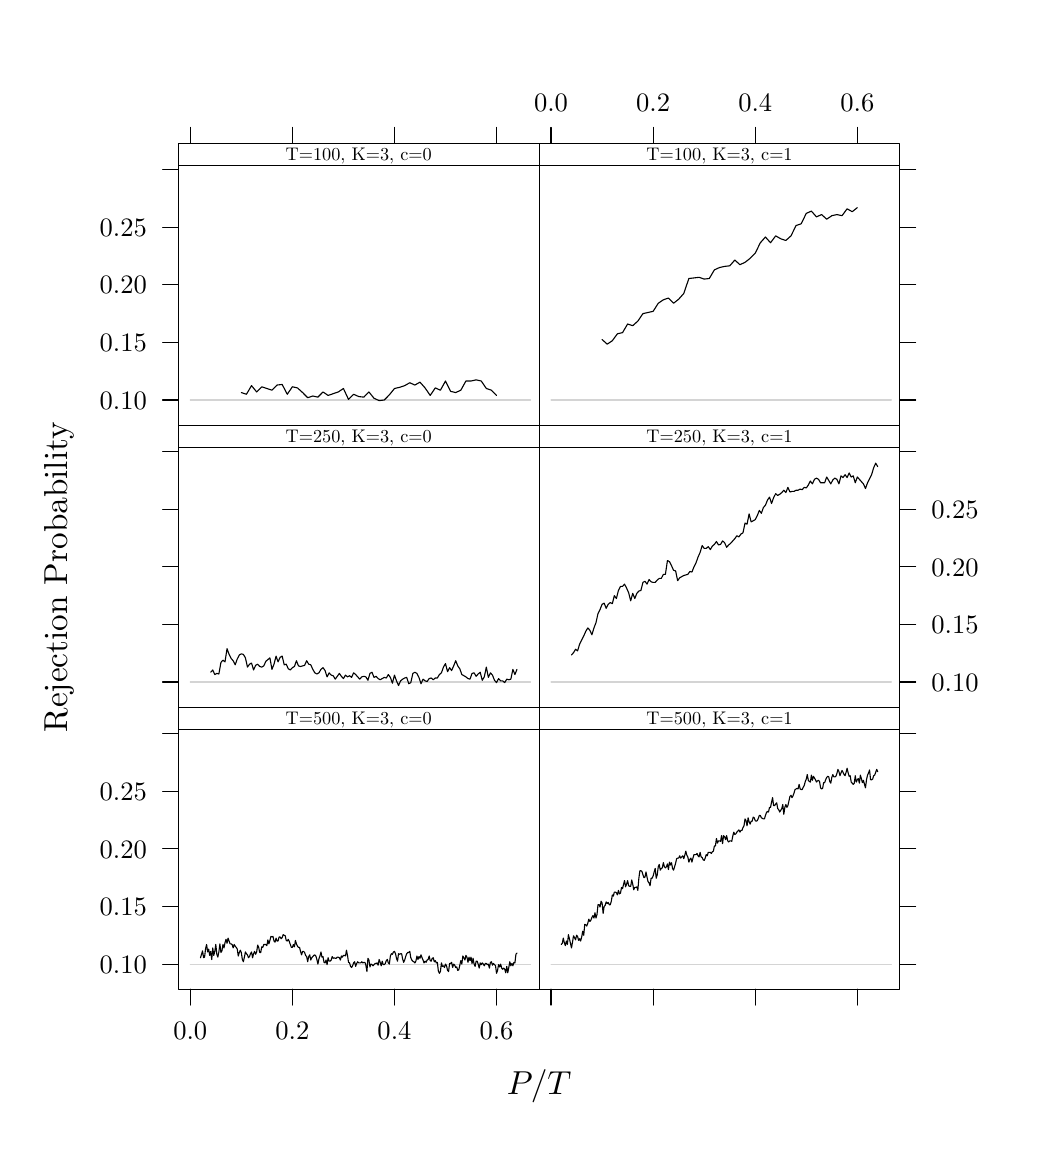
\begin{tikzpicture}[x=1pt,y=1pt]
\definecolor[named]{fillColor}{rgb}{1.00,1.00,1.00}
\path[use as bounding box,fill=fillColor,fill opacity=0.00] (0,0) rectangle (361.35,397.48);
\begin{scope}
\path[clip] (  0.00,  0.00) rectangle (361.35,397.48);

\path[] (  0.00,  0.00) rectangle (361.35,397.48);
\definecolor[named]{drawColor}{rgb}{0.00,0.00,0.00}

\node[text=drawColor,anchor=base,inner sep=0pt, outer sep=0pt, scale=  1.20] at (184.81, 12.04) {$P/T$};
\end{scope}
\begin{scope}
\path[clip] (  0.00,  0.00) rectangle (361.35,397.48);
\definecolor[named]{drawColor}{rgb}{0.00,0.00,0.00}

\node[text=drawColor,rotate= 90.00,anchor=base,inner sep=0pt, outer sep=0pt, scale=  1.20] at ( 14.29,198.90) {Rejection Probability};
\end{scope}
\begin{scope}
\path[clip] (  0.00,  0.00) rectangle (361.35,397.48);
\definecolor[named]{drawColor}{rgb}{0.00,0.00,0.00}

\path[draw=drawColor,line width= 0.4pt,line join=round,line cap=round] ( 54.44, 59.11) -- ( 48.75, 59.11);

\path[draw=drawColor,line width= 0.4pt,line join=round,line cap=round] ( 54.44, 79.93) -- ( 48.75, 79.93);

\path[draw=drawColor,line width= 0.4pt,line join=round,line cap=round] ( 54.44,100.74) -- ( 48.75,100.74);

\path[draw=drawColor,line width= 0.4pt,line join=round,line cap=round] ( 54.44,121.55) -- ( 48.75,121.55);

\path[draw=drawColor,line width= 0.4pt,line join=round,line cap=round] ( 54.44,142.37) -- ( 48.75,142.37);

\node[text=drawColor,anchor=base east,inner sep=0pt, outer sep=0pt, scale=  0.96] at ( 43.06, 55.81) {0.10};

\node[text=drawColor,anchor=base east,inner sep=0pt, outer sep=0pt, scale=  0.96] at ( 43.06, 76.62) {0.15};

\node[text=drawColor,anchor=base east,inner sep=0pt, outer sep=0pt, scale=  0.96] at ( 43.06, 97.43) {0.20};

\node[text=drawColor,anchor=base east,inner sep=0pt, outer sep=0pt, scale=  0.96] at ( 43.06,118.25) {0.25};
\end{scope}
\begin{scope}
\path[clip] (  0.00,  0.00) rectangle (361.35,397.48);
\definecolor[named]{drawColor}{rgb}{0.00,0.00,0.00}

\path[draw=drawColor,line width= 0.4pt,line join=round,line cap=round] ( 58.76, 50.02) -- ( 58.76, 44.32);

\path[draw=drawColor,line width= 0.4pt,line join=round,line cap=round] ( 95.65, 50.02) -- ( 95.65, 44.32);

\path[draw=drawColor,line width= 0.4pt,line join=round,line cap=round] (132.54, 50.02) -- (132.54, 44.32);

\path[draw=drawColor,line width= 0.4pt,line join=round,line cap=round] (169.42, 50.02) -- (169.42, 44.32);

\node[text=drawColor,anchor=base,inner sep=0pt, outer sep=0pt, scale=  0.96] at ( 58.76, 32.02) {0.0};

\node[text=drawColor,anchor=base,inner sep=0pt, outer sep=0pt, scale=  0.96] at ( 95.65, 32.02) {0.2};

\node[text=drawColor,anchor=base,inner sep=0pt, outer sep=0pt, scale=  0.96] at (132.54, 32.02) {0.4};

\node[text=drawColor,anchor=base,inner sep=0pt, outer sep=0pt, scale=  0.96] at (169.42, 32.02) {0.6};
\end{scope}
\begin{scope}
\path[clip] ( 54.44, 50.02) rectangle (184.81,143.97);
\definecolor[named]{drawColor}{rgb}{0.83,0.83,0.83}

\path[draw=drawColor,line width= 0.4pt,line join=round,line cap=round] ( 58.76, 59.11) --
	(181.72, 59.11);
\definecolor[named]{drawColor}{rgb}{0.00,0.00,0.00}

\path[draw=drawColor,line width= 0.4pt,line join=round,line cap=round] ( 62.45, 61.40) --
	( 62.82, 62.65) --
	( 63.19, 63.90) --
	( 63.56, 61.40) --
	( 63.92, 61.61) --
	( 64.29, 64.73) --
	( 64.66, 66.19) --
	( 65.03, 63.49) --
	( 65.40, 64.53) --
	( 65.77, 62.24) --
	( 66.14, 63.69) --
	( 66.51, 60.78) --
	( 66.88, 64.94) --
	( 67.24, 62.24) --
	( 67.61, 63.69) --
	( 67.98, 66.19) --
	( 68.35, 62.65) --
	( 68.72, 61.61) --
	( 69.09, 63.49) --
	( 69.46, 66.40) --
	( 69.83, 63.28) --
	( 70.20, 63.90) --
	( 70.56, 66.19) --
	( 70.93, 64.94) --
	( 71.30, 66.82) --
	( 71.67, 68.06) --
	( 72.04, 66.61) --
	( 72.41, 68.48) --
	( 72.78, 67.44) --
	( 73.15, 66.40) --
	( 73.52, 66.40) --
	( 73.88, 66.19) --
	( 74.25, 64.94) --
	( 74.62, 66.19) --
	( 74.99, 65.57) --
	( 75.36, 65.15) --
	( 75.73, 64.53) --
	( 76.10, 62.03) --
	( 76.47, 63.28) --
	( 76.84, 64.11) --
	( 77.20, 63.28) --
	( 77.57, 60.78) --
	( 77.94, 59.95) --
	( 78.31, 61.61) --
	( 78.68, 63.49) --
	( 79.05, 62.86) --
	( 79.42, 62.44) --
	( 79.79, 61.40) --
	( 80.16, 61.82) --
	( 80.52, 62.86) --
	( 80.89, 63.49) --
	( 81.26, 61.40) --
	( 81.63, 62.86) --
	( 82.00, 63.69) --
	( 82.37, 62.65) --
	( 82.74, 63.49) --
	( 83.11, 65.98) --
	( 83.48, 65.15) --
	( 83.84, 63.28) --
	( 84.21, 63.28) --
	( 84.58, 65.36) --
	( 84.95, 65.15) --
	( 85.32, 66.19) --
	( 85.69, 66.19) --
	( 86.06, 66.19) --
	( 86.43, 65.77) --
	( 86.79, 67.86) --
	( 87.16, 66.40) --
	( 87.53, 67.65) --
	( 87.90, 69.10) --
	( 88.27, 68.90) --
	( 88.64, 69.10) --
	( 89.01, 67.44) --
	( 89.38, 67.02) --
	( 89.75, 68.48) --
	( 90.11, 67.44) --
	( 90.48, 67.44) --
	( 90.85, 68.90) --
	( 91.22, 68.90) --
	( 91.59, 68.27) --
	( 91.96, 68.69) --
	( 92.33, 69.73) --
	( 92.70, 69.52) --
	( 93.07, 69.31) --
	( 93.43, 67.65) --
	( 93.80, 67.44) --
	( 94.17, 68.06) --
	( 94.54, 67.23) --
	( 94.91, 66.19) --
	( 95.28, 65.15) --
	( 95.65, 65.15) --
	( 96.02, 66.19) --
	( 96.39, 65.36) --
	( 96.75, 67.65) --
	( 97.12, 66.40) --
	( 97.49, 65.57) --
	( 97.86, 65.15) --
	( 98.23, 65.15) --
	( 98.60, 63.69) --
	( 98.97, 62.44) --
	( 99.34, 63.69) --
	( 99.71, 63.69) --
	(100.07, 63.28) --
	(100.44, 62.24) --
	(100.81, 61.82) --
	(101.18, 59.95) --
	(101.55, 61.82) --
	(101.92, 62.44) --
	(102.29, 60.57) --
	(102.66, 61.40) --
	(103.03, 61.82) --
	(103.39, 62.24) --
	(103.76, 62.44) --
	(104.13, 62.03) --
	(104.50, 60.78) --
	(104.87, 59.11) --
	(105.24, 60.99) --
	(105.61, 62.03) --
	(105.98, 63.49) --
	(106.35, 61.61) --
	(106.71, 61.82) --
	(107.08, 59.74) --
	(107.45, 59.53) --
	(107.82, 60.57) --
	(108.19, 58.91) --
	(108.56, 61.40) --
	(108.93, 60.16) --
	(109.30, 60.16) --
	(109.67, 60.57) --
	(110.03, 61.82) --
	(110.40, 61.20) --
	(110.77, 61.40) --
	(111.14, 61.20) --
	(111.51, 61.20) --
	(111.88, 61.61) --
	(112.25, 61.61) --
	(112.62, 61.40) --
	(112.99, 60.57) --
	(113.35, 62.03) --
	(113.72, 61.61) --
	(114.09, 62.24) --
	(114.46, 62.24) --
	(114.83, 62.03) --
	(115.20, 64.11) --
	(115.57, 62.24) --
	(115.94, 59.74) --
	(116.31, 59.53) --
	(116.67, 58.28) --
	(117.04, 57.87) --
	(117.41, 58.49) --
	(117.78, 59.53) --
	(118.15, 59.95) --
	(118.52, 58.28) --
	(118.89, 59.32) --
	(119.26, 59.95) --
	(119.63, 59.53) --
	(119.99, 59.53) --
	(120.36, 59.53) --
	(120.73, 59.95) --
	(121.10, 59.53) --
	(121.47, 59.74) --
	(121.84, 59.74) --
	(122.21, 58.70) --
	(122.58, 56.41) --
	(122.95, 61.20) --
	(123.31, 60.57) --
	(123.68, 58.07) --
	(124.05, 59.11) --
	(124.42, 58.91) --
	(124.79, 58.49) --
	(125.16, 58.91) --
	(125.53, 59.32) --
	(125.90, 59.32) --
	(126.27, 59.53) --
	(126.63, 58.70) --
	(127.00, 60.78) --
	(127.37, 59.74) --
	(127.74, 58.49) --
	(128.11, 60.16) --
	(128.48, 58.91) --
	(128.85, 58.91) --
	(129.22, 59.32) --
	(129.59, 60.36) --
	(129.95, 60.78) --
	(130.32, 59.53) --
	(130.69, 59.11) --
	(131.06, 62.03) --
	(131.43, 62.86) --
	(131.80, 62.65) --
	(132.17, 63.49) --
	(132.54, 63.69) --
	(132.91, 62.86) --
	(133.27, 61.20) --
	(133.64, 60.16) --
	(134.01, 62.86) --
	(134.38, 62.65) --
	(134.75, 62.86) --
	(135.12, 62.86) --
	(135.49, 60.99) --
	(135.86, 59.74) --
	(136.23, 60.57) --
	(136.59, 61.82) --
	(136.96, 62.86) --
	(137.33, 63.28) --
	(137.70, 63.28) --
	(138.07, 63.69) --
	(138.44, 61.40) --
	(138.81, 60.57) --
	(139.18, 60.16) --
	(139.55, 59.95) --
	(139.91, 59.53) --
	(140.28, 60.16) --
	(140.65, 62.03) --
	(141.02, 60.78) --
	(141.39, 61.82) --
	(141.76, 61.20) --
	(142.13, 62.44) --
	(142.50, 61.40) --
	(142.87, 60.57) --
	(143.23, 59.53) --
	(143.60, 60.16) --
	(143.97, 59.74) --
	(144.34, 60.57) --
	(144.71, 60.78) --
	(145.08, 62.03) --
	(145.45, 60.36) --
	(145.82, 60.16) --
	(146.19, 61.20) --
	(146.55, 61.40) --
	(146.92, 59.95) --
	(147.29, 60.36) --
	(147.66, 59.53) --
	(148.03, 59.74) --
	(148.40, 56.62) --
	(148.77, 55.78) --
	(149.14, 56.41) --
	(149.51, 59.53) --
	(149.87, 58.28) --
	(150.24, 58.49) --
	(150.61, 57.87) --
	(150.98, 59.11) --
	(151.35, 58.49) --
	(151.72, 56.83) --
	(152.09, 56.41) --
	(152.46, 59.32) --
	(152.83, 59.32) --
	(153.19, 59.74) --
	(153.56, 57.87) --
	(153.93, 59.11) --
	(154.30, 58.70) --
	(154.67, 57.87) --
	(155.04, 58.07) --
	(155.41, 56.83) --
	(155.78, 57.03) --
	(156.15, 58.70) --
	(156.51, 60.36) --
	(156.88, 59.11) --
	(157.25, 62.03) --
	(157.62, 61.40) --
	(157.99, 60.57) --
	(158.36, 62.24) --
	(158.73, 61.61) --
	(159.10, 59.74) --
	(159.47, 61.61) --
	(159.83, 60.36) --
	(160.20, 61.61) --
	(160.57, 59.32) --
	(160.94, 61.20) --
	(161.31, 59.11) --
	(161.68, 58.28) --
	(162.05, 60.16) --
	(162.42, 60.16) --
	(162.78, 59.11) --
	(163.15, 57.66) --
	(163.52, 59.53) --
	(163.89, 58.91) --
	(164.26, 59.53) --
	(164.63, 59.11) --
	(165.00, 58.49) --
	(165.37, 59.32) --
	(165.74, 59.32) --
	(166.10, 58.91) --
	(166.47, 59.11) --
	(166.84, 57.66) --
	(167.21, 59.74) --
	(167.58, 59.95) --
	(167.95, 58.70) --
	(168.32, 59.32) --
	(168.69, 58.91) --
	(169.06, 58.49) --
	(169.42, 55.78) --
	(169.79, 56.83) --
	(170.16, 58.91) --
	(170.53, 58.07) --
	(170.90, 59.11) --
	(171.27, 57.66) --
	(171.64, 57.24) --
	(172.01, 57.66) --
	(172.38, 57.24) --
	(172.74, 55.99) --
	(173.11, 58.28) --
	(173.48, 55.99) --
	(173.85, 57.87) --
	(174.22, 59.95) --
	(174.59, 58.49) --
	(174.96, 59.32) --
	(175.33, 58.49) --
	(175.70, 59.74) --
	(176.06, 59.53) --
	(176.43, 62.65) --
	(176.80, 63.07);
\end{scope}
\begin{scope}
\path[clip] (  0.00,  0.00) rectangle (361.35,397.48);
\definecolor[named]{drawColor}{rgb}{0.00,0.00,0.00}

\path[draw=drawColor,line width= 0.4pt,line join=round,line cap=round] ( 54.44, 50.02) rectangle (184.81,143.97);
\end{scope}
\begin{scope}
\path[clip] ( 54.44,143.97) rectangle (184.81,151.92);

\path[] ( 54.44,143.97) rectangle (184.81,151.92);
\definecolor[named]{drawColor}{rgb}{0.00,0.00,0.00}

\node[text=drawColor,anchor=base west,inner sep=0pt, outer sep=0pt, scale=  0.66] at ( 93.23,145.67) {T=500, K=3, c=0};
\end{scope}
\begin{scope}
\path[clip] (  0.00,  0.00) rectangle (361.35,397.48);
\definecolor[named]{drawColor}{rgb}{0.00,0.00,0.00}

\path[draw=drawColor,line width= 0.4pt,line join=round,line cap=round] ( 54.44,143.97) rectangle (184.81,151.92);
\end{scope}
\begin{scope}
\path[clip] (  0.00,  0.00) rectangle (361.35,397.48);
\definecolor[named]{drawColor}{rgb}{0.00,0.00,0.00}

\path[draw=drawColor,line width= 0.4pt,line join=round,line cap=round] (189.12, 50.02) -- (189.12, 44.32);

\path[draw=drawColor,line width= 0.4pt,line join=round,line cap=round] (226.01, 50.02) -- (226.01, 44.32);

\path[draw=drawColor,line width= 0.4pt,line join=round,line cap=round] (262.90, 50.02) -- (262.90, 44.32);

\path[draw=drawColor,line width= 0.4pt,line join=round,line cap=round] (299.79, 50.02) -- (299.79, 44.32);

\path[draw=drawColor,line width= 0.4pt,line join=round,line cap=round] (315.17, 59.11) -- (320.86, 59.11);

\path[draw=drawColor,line width= 0.4pt,line join=round,line cap=round] (315.17, 79.93) -- (320.86, 79.93);

\path[draw=drawColor,line width= 0.4pt,line join=round,line cap=round] (315.17,100.74) -- (320.86,100.74);

\path[draw=drawColor,line width= 0.4pt,line join=round,line cap=round] (315.17,121.55) -- (320.86,121.55);

\path[draw=drawColor,line width= 0.4pt,line join=round,line cap=round] (315.17,142.37) -- (320.86,142.37);
\end{scope}
\begin{scope}
\path[clip] (184.81, 50.02) rectangle (315.17,143.97);
\definecolor[named]{drawColor}{rgb}{0.83,0.83,0.83}

\path[draw=drawColor,line width= 0.4pt,line join=round,line cap=round] (189.12, 59.11) --
	(312.08, 59.11);
\definecolor[named]{drawColor}{rgb}{0.00,0.00,0.00}

\path[draw=drawColor,line width= 0.4pt,line join=round,line cap=round] (192.81, 66.19) --
	(193.18, 66.61) --
	(193.55, 68.48) --
	(193.92, 66.82) --
	(194.29, 65.77) --
	(194.66, 67.44) --
	(195.03, 66.19) --
	(195.39, 69.73) --
	(195.76, 68.27) --
	(196.13, 66.61) --
	(196.50, 64.94) --
	(196.87, 67.02) --
	(197.24, 69.31) --
	(197.61, 68.69) --
	(197.98, 67.86) --
	(198.35, 69.52) --
	(198.71, 69.10) --
	(199.08, 67.65) --
	(199.45, 68.27) --
	(199.82, 67.44) --
	(200.19, 68.90) --
	(200.56, 70.98) --
	(200.93, 69.52) --
	(201.30, 73.48) --
	(201.67, 73.27) --
	(202.03, 72.85) --
	(202.40, 73.89) --
	(202.77, 75.35) --
	(203.14, 74.52) --
	(203.51, 74.93) --
	(203.88, 75.97) --
	(204.25, 76.60) --
	(204.62, 75.76) --
	(204.99, 77.64) --
	(205.35, 75.76) --
	(205.72, 77.01) --
	(206.09, 80.55) --
	(206.46, 80.55) --
	(206.83, 79.72) --
	(207.20, 81.80) --
	(207.57, 81.18) --
	(207.94, 77.43) --
	(208.31, 79.93) --
	(208.67, 80.34) --
	(209.04, 81.59) --
	(209.41, 80.97) --
	(209.78, 81.38) --
	(210.15, 80.55) --
	(210.52, 80.55) --
	(210.89, 81.80) --
	(211.26, 84.09) --
	(211.63, 83.67) --
	(211.99, 85.13) --
	(212.36, 85.13) --
	(212.73, 84.92) --
	(213.10, 84.09) --
	(213.47, 85.75) --
	(213.84, 84.51) --
	(214.21, 84.71) --
	(214.58, 86.80) --
	(214.95, 86.38) --
	(215.31, 87.84) --
	(215.68, 89.29) --
	(216.05, 87.00) --
	(216.42, 88.04) --
	(216.79, 89.29) --
	(217.16, 87.42) --
	(217.53, 87.21) --
	(217.90, 87.21) --
	(218.27, 89.50) --
	(218.63, 88.04) --
	(219.00, 85.96) --
	(219.37, 86.80) --
	(219.74, 86.80) --
	(220.11, 87.00) --
	(220.48, 85.75) --
	(220.85, 90.13) --
	(221.22, 92.83) --
	(221.58, 92.83) --
	(221.95, 92.62) --
	(222.32, 91.37) --
	(222.69, 90.33) --
	(223.06, 90.54) --
	(223.43, 92.41) --
	(223.80, 90.54) --
	(224.17, 88.88) --
	(224.54, 88.46) --
	(224.90, 87.42) --
	(225.27, 90.13) --
	(225.64, 90.13) --
	(226.01, 90.96) --
	(226.38, 92.41) --
	(226.75, 93.66) --
	(227.12, 90.13) --
	(227.49, 91.37) --
	(227.86, 94.29) --
	(228.22, 95.12) --
	(228.59, 93.04) --
	(228.96, 93.66) --
	(229.33, 93.87) --
	(229.70, 95.75) --
	(230.07, 94.29) --
	(230.44, 93.87) --
	(230.81, 94.29) --
	(231.18, 95.33) --
	(231.54, 93.25) --
	(231.91, 95.95) --
	(232.28, 94.91) --
	(232.65, 95.75) --
	(233.02, 93.66) --
	(233.39, 93.04) --
	(233.76, 94.29) --
	(234.13, 95.54) --
	(234.50, 97.20) --
	(234.86, 97.41) --
	(235.23, 97.41) --
	(235.60, 98.24) --
	(235.97, 97.41) --
	(236.34, 97.83) --
	(236.71, 98.24) --
	(237.08, 97.20) --
	(237.45, 98.45) --
	(237.82, 99.91) --
	(238.18, 98.45) --
	(238.55, 97.83) --
	(238.92, 95.95) --
	(239.29, 96.99) --
	(239.66, 97.41) --
	(240.03, 95.95) --
	(240.40, 97.41) --
	(240.77, 98.66) --
	(241.14, 98.66) --
	(241.50, 98.66) --
	(241.87, 99.08) --
	(242.24, 98.24) --
	(242.61, 97.83) --
	(242.98, 99.49) --
	(243.35, 97.83) --
	(243.72, 97.62) --
	(244.09, 96.79) --
	(244.46, 96.58) --
	(244.82, 97.41) --
	(245.19, 98.66) --
	(245.56, 98.24) --
	(245.93, 99.49) --
	(246.30, 99.49) --
	(246.67, 99.49) --
	(247.04, 99.08) --
	(247.41, 99.70) --
	(247.78, 99.91) --
	(248.14,101.78) --
	(248.51,101.78) --
	(248.88,104.49) --
	(249.25,102.82) --
	(249.62,103.65) --
	(249.99,103.65) --
	(250.36,103.45) --
	(250.73,105.53) --
	(251.10,102.61) --
	(251.46,105.53) --
	(251.83,105.11) --
	(252.20,104.07) --
	(252.57,105.53) --
	(252.94,103.65) --
	(253.31,103.24) --
	(253.68,103.65) --
	(254.05,103.65) --
	(254.42,103.45) --
	(254.78,105.32) --
	(255.15,106.78) --
	(255.52,105.94) --
	(255.89,106.15) --
	(256.26,106.78) --
	(256.63,107.19) --
	(257.00,107.61) --
	(257.37,106.78) --
	(257.74,107.40) --
	(258.10,107.40) --
	(258.47,108.44) --
	(258.84,109.07) --
	(259.21,111.56) --
	(259.58,110.94) --
	(259.95,109.07) --
	(260.32,111.98) --
	(260.69,110.52) --
	(261.06,109.69) --
	(261.42,110.73) --
	(261.79,110.73) --
	(262.16,112.19) --
	(262.53,111.98) --
	(262.90,110.94) --
	(263.27,110.73) --
	(263.64,110.94) --
	(264.01,111.77) --
	(264.38,112.81) --
	(264.74,112.81) --
	(265.11,111.98) --
	(265.48,111.77) --
	(265.85,111.56) --
	(266.22,111.56) --
	(266.59,112.81) --
	(266.96,113.85) --
	(267.33,114.27) --
	(267.70,114.06) --
	(268.06,115.73) --
	(268.43,115.73) --
	(268.80,117.60) --
	(269.17,119.26) --
	(269.54,116.35) --
	(269.91,116.35) --
	(270.28,116.97) --
	(270.65,117.39) --
	(271.02,115.31) --
	(271.38,114.89) --
	(271.75,114.06) --
	(272.12,114.68) --
	(272.49,115.31) --
	(272.86,116.77) --
	(273.23,113.23) --
	(273.60,115.73) --
	(273.97,116.77) --
	(274.34,115.73) --
	(274.70,116.35) --
	(275.07,118.01) --
	(275.44,119.68) --
	(275.81,120.10) --
	(276.18,119.26) --
	(276.55,119.89) --
	(276.92,120.93) --
	(277.29,122.18) --
	(277.66,122.39) --
	(278.02,122.59) --
	(278.39,122.39) --
	(278.76,124.05) --
	(279.13,122.39) --
	(279.50,122.18) --
	(279.87,122.18) --
	(280.24,123.01) --
	(280.61,123.63) --
	(280.98,125.09) --
	(281.34,125.92) --
	(281.71,127.59) --
	(282.08,125.51) --
	(282.45,125.09) --
	(282.82,124.88) --
	(283.19,127.38) --
	(283.56,125.51) --
	(283.93,126.96) --
	(284.30,126.34) --
	(284.66,125.72) --
	(285.03,124.88) --
	(285.40,125.30) --
	(285.77,125.51) --
	(286.14,125.09) --
	(286.51,122.80) --
	(286.88,122.39) --
	(287.25,122.59) --
	(287.62,124.67) --
	(287.98,124.67) --
	(288.35,125.72) --
	(288.72,126.55) --
	(289.09,126.96) --
	(289.46,126.76) --
	(289.83,125.09) --
	(290.20,124.47) --
	(290.57,126.55) --
	(290.94,127.59) --
	(291.30,126.76) --
	(291.67,126.76) --
	(292.04,126.96) --
	(292.41,128.00) --
	(292.78,129.46) --
	(293.15,128.63) --
	(293.52,127.17) --
	(293.89,128.21) --
	(294.26,129.05) --
	(294.62,128.42) --
	(294.99,127.59) --
	(295.36,127.17) --
	(295.73,128.42) --
	(296.10,129.88) --
	(296.47,128.21) --
	(296.84,126.96) --
	(297.21,127.17) --
	(297.58,124.88) --
	(297.94,124.47) --
	(298.31,124.05) --
	(298.68,124.47) --
	(299.05,127.17) --
	(299.42,124.88) --
	(299.79,125.72) --
	(300.16,126.13) --
	(300.53,124.47) --
	(300.89,127.38) --
	(301.26,126.13) --
	(301.63,124.67) --
	(302.00,125.51) --
	(302.37,124.05) --
	(302.74,122.80) --
	(303.11,125.72) --
	(303.48,127.38) --
	(303.85,128.21) --
	(304.21,129.25) --
	(304.58,125.72) --
	(304.95,125.72) --
	(305.32,125.92) --
	(305.69,127.17) --
	(306.06,127.38) --
	(306.43,128.42) --
	(306.80,129.46) --
	(307.17,128.63);
\end{scope}
\begin{scope}
\path[clip] (  0.00,  0.00) rectangle (361.35,397.48);
\definecolor[named]{drawColor}{rgb}{0.00,0.00,0.00}

\path[draw=drawColor,line width= 0.4pt,line join=round,line cap=round] (184.81, 50.02) rectangle (315.17,143.97);
\end{scope}
\begin{scope}
\path[clip] (184.81,143.97) rectangle (315.17,151.92);

\path[] (184.81,143.97) rectangle (315.17,151.92);
\definecolor[named]{drawColor}{rgb}{0.00,0.00,0.00}

\node[text=drawColor,anchor=base west,inner sep=0pt, outer sep=0pt, scale=  0.66] at (223.60,145.67) {T=500, K=3, c=1};
\end{scope}
\begin{scope}
\path[clip] (  0.00,  0.00) rectangle (361.35,397.48);
\definecolor[named]{drawColor}{rgb}{0.00,0.00,0.00}

\path[draw=drawColor,line width= 0.4pt,line join=round,line cap=round] (184.81,143.97) rectangle (315.17,151.92);
\end{scope}
\begin{scope}
\path[clip] (  0.00,  0.00) rectangle (361.35,397.48);
\definecolor[named]{drawColor}{rgb}{0.00,0.00,0.00}

\path[draw=drawColor,line width= 0.4pt,line join=round,line cap=round] ( 54.44,161.02) -- ( 48.75,161.02);

\path[draw=drawColor,line width= 0.4pt,line join=round,line cap=round] ( 54.44,181.83) -- ( 48.75,181.83);

\path[draw=drawColor,line width= 0.4pt,line join=round,line cap=round] ( 54.44,202.65) -- ( 48.75,202.65);

\path[draw=drawColor,line width= 0.4pt,line join=round,line cap=round] ( 54.44,223.46) -- ( 48.75,223.46);

\path[draw=drawColor,line width= 0.4pt,line join=round,line cap=round] ( 54.44,244.27) -- ( 48.75,244.27);
\end{scope}
\begin{scope}
\path[clip] ( 54.44,151.92) rectangle (184.81,245.88);
\definecolor[named]{drawColor}{rgb}{0.83,0.83,0.83}

\path[draw=drawColor,line width= 0.4pt,line join=round,line cap=round] ( 58.76,161.02) --
	(181.72,161.02);
\definecolor[named]{drawColor}{rgb}{0.00,0.00,0.00}

\path[draw=drawColor,line width= 0.4pt,line join=round,line cap=round] ( 66.14,164.56) --
	( 66.88,165.39) --
	( 67.61,163.73) --
	( 68.35,164.14) --
	( 69.09,163.93) --
	( 69.83,168.10) --
	( 70.56,168.93) --
	( 71.30,168.31) --
	( 72.04,173.09) --
	( 72.78,171.01) --
	( 73.52,169.55) --
	( 74.25,168.72) --
	( 74.99,167.26) --
	( 75.73,169.35) --
	( 76.47,170.80) --
	( 77.20,171.22) --
	( 77.94,171.01) --
	( 78.68,169.76) --
	( 79.42,166.43) --
	( 80.16,167.47) --
	( 80.89,167.89) --
	( 81.63,165.39) --
	( 82.37,167.06) --
	( 83.11,167.47) --
	( 83.84,166.64) --
	( 84.58,166.43) --
	( 85.32,166.85) --
	( 86.06,168.51) --
	( 86.79,169.14) --
	( 87.53,169.76) --
	( 88.27,165.60) --
	( 89.01,167.47) --
	( 89.75,170.39) --
	( 90.48,168.31) --
	( 91.22,169.97) --
	( 91.96,170.39) --
	( 92.70,167.26) --
	( 93.43,167.47) --
	( 94.17,165.81) --
	( 94.91,165.39) --
	( 95.65,166.22) --
	( 96.39,166.64) --
	( 97.12,168.72) --
	( 97.86,166.85) --
	( 98.60,166.64) --
	( 99.34,166.85) --
	(100.07,167.06) --
	(100.81,168.72) --
	(101.55,167.47) --
	(102.29,167.26) --
	(103.03,165.60) --
	(103.76,164.35) --
	(104.50,163.93) --
	(105.24,164.35) --
	(105.98,165.60) --
	(106.71,166.22) --
	(107.45,165.18) --
	(108.19,162.89) --
	(108.93,164.35) --
	(109.67,163.52) --
	(110.40,163.31) --
	(111.14,162.06) --
	(111.88,163.10) --
	(112.62,164.14) --
	(113.35,163.10) --
	(114.09,162.27) --
	(114.83,163.52) --
	(115.57,162.89) --
	(116.31,163.31) --
	(117.04,162.69) --
	(117.78,164.35) --
	(118.52,163.73) --
	(119.26,162.89) --
	(119.99,162.06) --
	(120.73,162.89) --
	(121.47,163.10) --
	(122.21,162.89) --
	(122.95,161.65) --
	(123.68,164.14) --
	(124.42,164.56) --
	(125.16,162.69) --
	(125.90,163.10) --
	(126.63,162.27) --
	(127.37,161.85) --
	(128.11,162.27) --
	(128.85,162.69) --
	(129.59,162.48) --
	(130.32,163.73) --
	(131.06,162.69) --
	(131.80,160.60) --
	(132.54,163.52) --
	(133.27,161.44) --
	(134.01,159.77) --
	(134.75,161.44) --
	(135.49,162.06) --
	(136.23,162.48) --
	(136.96,162.69) --
	(137.70,160.40) --
	(138.44,160.81) --
	(139.18,164.14) --
	(139.91,164.56) --
	(140.65,164.14) --
	(141.39,162.69) --
	(142.13,160.40) --
	(142.87,162.06) --
	(143.60,161.44) --
	(144.34,161.23) --
	(145.08,162.27) --
	(145.82,162.48) --
	(146.55,161.85) --
	(147.29,162.48) --
	(148.03,162.48) --
	(148.77,163.73) --
	(149.51,164.35) --
	(150.24,166.43) --
	(150.98,167.68) --
	(151.72,164.77) --
	(152.46,166.22) --
	(153.19,165.18) --
	(153.93,166.85) --
	(154.67,168.72) --
	(155.41,166.85) --
	(156.15,165.81) --
	(156.88,163.73) --
	(157.62,163.31) --
	(158.36,162.89) --
	(159.10,162.27) --
	(159.83,162.06) --
	(160.57,164.14) --
	(161.31,164.35) --
	(162.05,163.10) --
	(162.78,163.93) --
	(163.52,164.56) --
	(164.26,161.65) --
	(165.00,162.89) --
	(165.74,166.43) --
	(166.47,162.69) --
	(167.21,164.35) --
	(167.95,163.52) --
	(168.69,161.65) --
	(169.42,160.81) --
	(170.16,162.27) --
	(170.90,161.44) --
	(171.64,161.44) --
	(172.38,160.81) --
	(173.11,162.06) --
	(173.85,161.85) --
	(174.59,162.06) --
	(175.33,165.60) --
	(176.06,163.73) --
	(176.80,165.60);
\end{scope}
\begin{scope}
\path[clip] (  0.00,  0.00) rectangle (361.35,397.48);
\definecolor[named]{drawColor}{rgb}{0.00,0.00,0.00}

\path[draw=drawColor,line width= 0.4pt,line join=round,line cap=round] ( 54.44,151.92) rectangle (184.81,245.88);
\end{scope}
\begin{scope}
\path[clip] ( 54.44,245.88) rectangle (184.81,253.83);

\path[] ( 54.44,245.88) rectangle (184.81,253.83);
\definecolor[named]{drawColor}{rgb}{0.00,0.00,0.00}

\node[text=drawColor,anchor=base west,inner sep=0pt, outer sep=0pt, scale=  0.66] at ( 93.23,247.58) {T=250, K=3, c=0};
\end{scope}
\begin{scope}
\path[clip] (  0.00,  0.00) rectangle (361.35,397.48);
\definecolor[named]{drawColor}{rgb}{0.00,0.00,0.00}

\path[draw=drawColor,line width= 0.4pt,line join=round,line cap=round] ( 54.44,245.88) rectangle (184.81,253.83);
\end{scope}
\begin{scope}
\path[clip] (  0.00,  0.00) rectangle (361.35,397.48);
\definecolor[named]{drawColor}{rgb}{0.00,0.00,0.00}

\path[draw=drawColor,line width= 0.4pt,line join=round,line cap=round] (315.17,161.02) -- (320.86,161.02);

\path[draw=drawColor,line width= 0.4pt,line join=round,line cap=round] (315.17,181.83) -- (320.86,181.83);

\path[draw=drawColor,line width= 0.4pt,line join=round,line cap=round] (315.17,202.65) -- (320.86,202.65);

\path[draw=drawColor,line width= 0.4pt,line join=round,line cap=round] (315.17,223.46) -- (320.86,223.46);

\path[draw=drawColor,line width= 0.4pt,line join=round,line cap=round] (315.17,244.27) -- (320.86,244.27);

\node[text=drawColor,anchor=base west,inner sep=0pt, outer sep=0pt, scale=  0.96] at (326.55,157.72) {0.10};

\node[text=drawColor,anchor=base west,inner sep=0pt, outer sep=0pt, scale=  0.96] at (326.55,178.53) {0.15};

\node[text=drawColor,anchor=base west,inner sep=0pt, outer sep=0pt, scale=  0.96] at (326.55,199.34) {0.20};

\node[text=drawColor,anchor=base west,inner sep=0pt, outer sep=0pt, scale=  0.96] at (326.55,220.15) {0.25};
\end{scope}
\begin{scope}
\path[clip] (184.81,151.92) rectangle (315.17,245.88);
\definecolor[named]{drawColor}{rgb}{0.83,0.83,0.83}

\path[draw=drawColor,line width= 0.4pt,line join=round,line cap=round] (189.12,161.02) --
	(312.08,161.02);
\definecolor[named]{drawColor}{rgb}{0.00,0.00,0.00}

\path[draw=drawColor,line width= 0.4pt,line join=round,line cap=round] (196.50,170.80) --
	(197.24,171.64) --
	(197.98,172.88) --
	(198.71,172.26) --
	(199.45,174.76) --
	(200.19,176.21) --
	(200.93,177.67) --
	(201.67,179.34) --
	(202.40,180.58) --
	(203.14,179.75) --
	(203.88,178.09) --
	(204.62,180.58) --
	(205.35,182.46) --
	(206.09,185.79) --
	(206.83,187.24) --
	(207.57,189.12) --
	(208.31,189.53) --
	(209.04,187.66) --
	(209.78,189.12) --
	(210.52,189.74) --
	(211.26,189.33) --
	(211.99,192.24) --
	(212.73,191.20) --
	(213.47,194.11) --
	(214.21,195.57) --
	(214.95,195.57) --
	(215.68,196.40) --
	(216.42,194.95) --
	(217.16,193.28) --
	(217.90,190.37) --
	(218.63,193.07) --
	(219.37,191.20) --
	(220.11,193.07) --
	(220.85,193.90) --
	(221.58,194.11) --
	(222.32,197.03) --
	(223.06,197.44) --
	(223.80,196.40) --
	(224.54,198.07) --
	(225.27,197.23) --
	(226.01,197.03) --
	(226.75,197.03) --
	(227.49,197.86) --
	(228.22,198.48) --
	(228.96,198.48) --
	(229.70,199.94) --
	(230.44,199.94) --
	(231.18,204.94) --
	(231.91,204.52) --
	(232.65,203.06) --
	(233.39,201.40) --
	(234.13,201.19) --
	(234.86,197.65) --
	(235.60,198.69) --
	(236.34,199.11) --
	(237.08,199.52) --
	(237.82,199.73) --
	(238.55,199.94) --
	(239.29,200.98) --
	(240.03,200.77) --
	(240.77,202.65) --
	(241.50,204.10) --
	(242.24,206.18) --
	(242.98,207.85) --
	(243.72,210.35) --
	(244.46,209.31) --
	(245.19,209.31) --
	(245.93,209.93) --
	(246.67,208.89) --
	(247.41,210.14) --
	(248.14,210.76) --
	(248.88,211.80) --
	(249.62,210.56) --
	(250.36,210.76) --
	(251.10,212.01) --
	(251.83,211.39) --
	(252.57,209.72) --
	(253.31,210.56) --
	(254.05,211.18) --
	(254.78,212.01) --
	(255.52,212.84) --
	(256.26,213.89) --
	(257.00,213.47) --
	(257.74,214.51) --
	(258.47,214.93) --
	(259.21,218.46) --
	(259.95,218.05) --
	(260.69,221.79) --
	(261.42,218.88) --
	(262.16,219.30) --
	(262.90,219.71) --
	(263.64,221.17) --
	(264.38,223.04) --
	(265.11,222.00) --
	(265.85,224.08) --
	(266.59,224.92) --
	(267.33,226.79) --
	(268.06,227.83) --
	(268.80,225.54) --
	(269.54,227.62) --
	(270.28,229.08) --
	(271.02,228.45) --
	(271.75,228.87) --
	(272.49,229.49) --
	(273.23,230.33) --
	(273.97,229.49) --
	(274.70,231.37) --
	(275.44,229.70) --
	(276.18,229.91) --
	(276.92,229.91) --
	(277.66,230.33) --
	(278.39,230.33) --
	(279.13,230.74) --
	(279.87,230.54) --
	(280.61,231.37) --
	(281.34,231.16) --
	(282.08,232.20) --
	(282.82,233.66) --
	(283.56,232.62) --
	(284.30,234.28) --
	(285.03,234.70) --
	(285.77,234.28) --
	(286.51,233.03) --
	(287.25,233.03) --
	(287.98,233.03) --
	(288.72,235.11) --
	(289.46,233.87) --
	(290.20,232.62) --
	(290.94,234.07) --
	(291.67,234.70) --
	(292.41,234.28) --
	(293.15,232.62) --
	(293.89,235.53) --
	(294.62,234.91) --
	(295.36,235.95) --
	(296.10,234.91) --
	(296.84,236.57) --
	(297.58,235.11) --
	(298.31,235.53) --
	(299.05,233.03) --
	(299.79,235.11) --
	(300.53,234.28) --
	(301.26,233.45) --
	(302.00,232.62) --
	(302.74,230.95) --
	(303.48,233.03) --
	(304.21,234.49) --
	(304.95,235.95) --
	(305.69,238.44) --
	(306.43,240.11) --
	(307.17,238.86);
\end{scope}
\begin{scope}
\path[clip] (  0.00,  0.00) rectangle (361.35,397.48);
\definecolor[named]{drawColor}{rgb}{0.00,0.00,0.00}

\path[draw=drawColor,line width= 0.4pt,line join=round,line cap=round] (184.81,151.92) rectangle (315.17,245.88);
\end{scope}
\begin{scope}
\path[clip] (184.81,245.88) rectangle (315.17,253.83);

\path[] (184.81,245.88) rectangle (315.17,253.83);
\definecolor[named]{drawColor}{rgb}{0.00,0.00,0.00}

\node[text=drawColor,anchor=base west,inner sep=0pt, outer sep=0pt, scale=  0.66] at (223.60,247.58) {T=250, K=3, c=1};
\end{scope}
\begin{scope}
\path[clip] (  0.00,  0.00) rectangle (361.35,397.48);
\definecolor[named]{drawColor}{rgb}{0.00,0.00,0.00}

\path[draw=drawColor,line width= 0.4pt,line join=round,line cap=round] (184.81,245.88) rectangle (315.17,253.83);
\end{scope}
\begin{scope}
\path[clip] (  0.00,  0.00) rectangle (361.35,397.48);
\definecolor[named]{drawColor}{rgb}{0.00,0.00,0.00}

\path[draw=drawColor,line width= 0.4pt,line join=round,line cap=round] ( 58.76,355.73) -- ( 58.76,361.42);

\path[draw=drawColor,line width= 0.4pt,line join=round,line cap=round] ( 95.65,355.73) -- ( 95.65,361.42);

\path[draw=drawColor,line width= 0.4pt,line join=round,line cap=round] (132.54,355.73) -- (132.54,361.42);

\path[draw=drawColor,line width= 0.4pt,line join=round,line cap=round] (169.42,355.73) -- (169.42,361.42);
\end{scope}
\begin{scope}
\path[clip] (  0.00,  0.00) rectangle (361.35,397.48);
\definecolor[named]{drawColor}{rgb}{0.00,0.00,0.00}

\path[draw=drawColor,line width= 0.4pt,line join=round,line cap=round] ( 54.44,262.93) -- ( 48.75,262.93);

\path[draw=drawColor,line width= 0.4pt,line join=round,line cap=round] ( 54.44,283.74) -- ( 48.75,283.74);

\path[draw=drawColor,line width= 0.4pt,line join=round,line cap=round] ( 54.44,304.55) -- ( 48.75,304.55);

\path[draw=drawColor,line width= 0.4pt,line join=round,line cap=round] ( 54.44,325.37) -- ( 48.75,325.37);

\path[draw=drawColor,line width= 0.4pt,line join=round,line cap=round] ( 54.44,346.18) -- ( 48.75,346.18);

\node[text=drawColor,anchor=base east,inner sep=0pt, outer sep=0pt, scale=  0.96] at ( 43.06,259.62) {0.10};

\node[text=drawColor,anchor=base east,inner sep=0pt, outer sep=0pt, scale=  0.96] at ( 43.06,280.43) {0.15};

\node[text=drawColor,anchor=base east,inner sep=0pt, outer sep=0pt, scale=  0.96] at ( 43.06,301.25) {0.20};

\node[text=drawColor,anchor=base east,inner sep=0pt, outer sep=0pt, scale=  0.96] at ( 43.06,322.06) {0.25};
\end{scope}
\begin{scope}
\path[clip] ( 54.44,253.83) rectangle (184.81,347.78);
\definecolor[named]{drawColor}{rgb}{0.83,0.83,0.83}

\path[draw=drawColor,line width= 0.4pt,line join=round,line cap=round] ( 58.76,262.93) --
	(181.72,262.93);
\definecolor[named]{drawColor}{rgb}{0.00,0.00,0.00}

\path[draw=drawColor,line width= 0.4pt,line join=round,line cap=round] ( 77.20,265.63) --
	( 79.05,265.01) --
	( 80.89,268.13) --
	( 82.74,265.84) --
	( 84.58,267.71) --
	( 86.43,267.09) --
	( 88.27,266.47) --
	( 90.11,268.34) --
	( 91.96,268.55) --
	( 93.80,265.01) --
	( 95.65,267.71) --
	( 97.49,267.30) --
	( 99.34,265.63) --
	(101.18,263.76) --
	(103.03,264.38) --
	(104.87,263.97) --
	(106.71,265.84) --
	(108.56,264.59) --
	(110.40,265.22) --
	(112.25,265.84) --
	(114.09,267.09) --
	(115.94,263.14) --
	(117.78,265.01) --
	(119.63,264.18) --
	(121.47,263.97) --
	(123.31,265.84) --
	(125.16,263.55) --
	(127.00,262.72) --
	(128.85,262.93) --
	(130.69,264.80) --
	(132.54,267.09) --
	(134.38,267.51) --
	(136.23,268.13) --
	(138.07,269.17) --
	(139.91,268.34) --
	(141.76,269.38) --
	(143.60,267.30) --
	(145.45,264.59) --
	(147.29,267.30) --
	(149.14,266.47) --
	(150.98,269.80) --
	(152.83,266.05) --
	(154.67,265.63) --
	(156.51,266.47) --
	(158.36,269.80) --
	(160.20,269.80) --
	(162.05,270.21) --
	(163.89,269.80) --
	(165.74,267.09) --
	(167.58,266.47) --
	(169.42,264.59);
\end{scope}
\begin{scope}
\path[clip] (  0.00,  0.00) rectangle (361.35,397.48);
\definecolor[named]{drawColor}{rgb}{0.00,0.00,0.00}

\path[draw=drawColor,line width= 0.4pt,line join=round,line cap=round] ( 54.44,253.83) rectangle (184.81,347.78);
\end{scope}
\begin{scope}
\path[clip] ( 54.44,347.78) rectangle (184.81,355.73);

\path[] ( 54.44,347.78) rectangle (184.81,355.73);
\definecolor[named]{drawColor}{rgb}{0.00,0.00,0.00}

\node[text=drawColor,anchor=base west,inner sep=0pt, outer sep=0pt, scale=  0.66] at ( 93.23,349.49) {T=100, K=3, c=0};
\end{scope}
\begin{scope}
\path[clip] (  0.00,  0.00) rectangle (361.35,397.48);
\definecolor[named]{drawColor}{rgb}{0.00,0.00,0.00}

\path[draw=drawColor,line width= 0.4pt,line join=round,line cap=round] ( 54.44,347.78) rectangle (184.81,355.73);
\end{scope}
\begin{scope}
\path[clip] (  0.00,  0.00) rectangle (361.35,397.48);
\definecolor[named]{drawColor}{rgb}{0.00,0.00,0.00}

\path[draw=drawColor,line width= 0.4pt,line join=round,line cap=round] (189.12,355.73) -- (189.12,361.42);

\path[draw=drawColor,line width= 0.4pt,line join=round,line cap=round] (226.01,355.73) -- (226.01,361.42);

\path[draw=drawColor,line width= 0.4pt,line join=round,line cap=round] (262.90,355.73) -- (262.90,361.42);

\path[draw=drawColor,line width= 0.4pt,line join=round,line cap=round] (299.79,355.73) -- (299.79,361.42);

\node[text=drawColor,anchor=base,inner sep=0pt, outer sep=0pt, scale=  0.96] at (189.12,367.12) {0.0};

\node[text=drawColor,anchor=base,inner sep=0pt, outer sep=0pt, scale=  0.96] at (226.01,367.12) {0.2};

\node[text=drawColor,anchor=base,inner sep=0pt, outer sep=0pt, scale=  0.96] at (262.90,367.12) {0.4};

\node[text=drawColor,anchor=base,inner sep=0pt, outer sep=0pt, scale=  0.96] at (299.79,367.12) {0.6};
\end{scope}
\begin{scope}
\path[clip] (  0.00,  0.00) rectangle (361.35,397.48);
\definecolor[named]{drawColor}{rgb}{0.00,0.00,0.00}

\path[draw=drawColor,line width= 0.4pt,line join=round,line cap=round] (315.17,262.93) -- (320.86,262.93);

\path[draw=drawColor,line width= 0.4pt,line join=round,line cap=round] (315.17,283.74) -- (320.86,283.74);

\path[draw=drawColor,line width= 0.4pt,line join=round,line cap=round] (315.17,304.55) -- (320.86,304.55);

\path[draw=drawColor,line width= 0.4pt,line join=round,line cap=round] (315.17,325.37) -- (320.86,325.37);

\path[draw=drawColor,line width= 0.4pt,line join=round,line cap=round] (315.17,346.18) -- (320.86,346.18);
\end{scope}
\begin{scope}
\path[clip] (184.81,253.83) rectangle (315.17,347.78);
\definecolor[named]{drawColor}{rgb}{0.83,0.83,0.83}

\path[draw=drawColor,line width= 0.4pt,line join=round,line cap=round] (189.12,262.93) --
	(312.08,262.93);
\definecolor[named]{drawColor}{rgb}{0.00,0.00,0.00}

\path[draw=drawColor,line width= 0.4pt,line join=round,line cap=round] (207.57,284.78) --
	(209.41,283.12) --
	(211.26,284.36) --
	(213.10,286.86) --
	(214.95,287.28) --
	(216.79,290.40) --
	(218.63,289.78) --
	(220.48,291.44) --
	(222.32,294.15) --
	(224.17,294.56) --
	(226.01,294.98) --
	(227.86,297.89) --
	(229.70,299.14) --
	(231.54,299.77) --
	(233.39,297.89) --
	(235.23,299.35) --
	(237.08,301.43) --
	(238.92,306.84) --
	(240.77,307.05) --
	(242.61,307.26) --
	(244.46,306.63) --
	(246.30,306.84) --
	(248.14,309.96) --
	(249.99,310.80) --
	(251.83,311.21) --
	(253.68,311.42) --
	(255.52,313.50) --
	(257.37,311.84) --
	(259.21,312.67) --
	(261.06,314.13) --
	(262.90,316.00) --
	(264.74,319.75) --
	(266.59,321.83) --
	(268.43,319.75) --
	(270.28,322.24) --
	(272.12,321.20) --
	(273.97,320.58) --
	(275.81,322.24) --
	(277.66,325.99) --
	(279.50,326.61) --
	(281.34,330.36) --
	(283.19,331.19) --
	(285.03,329.11) --
	(286.88,329.94) --
	(288.72,328.28) --
	(290.57,329.53) --
	(292.41,329.94) --
	(294.26,329.53) --
	(296.10,332.03) --
	(297.94,330.98) --
	(299.79,332.44);
\end{scope}
\begin{scope}
\path[clip] (  0.00,  0.00) rectangle (361.35,397.48);
\definecolor[named]{drawColor}{rgb}{0.00,0.00,0.00}

\path[draw=drawColor,line width= 0.4pt,line join=round,line cap=round] (184.81,253.83) rectangle (315.17,347.78);
\end{scope}
\begin{scope}
\path[clip] (184.81,347.78) rectangle (315.17,355.73);

\path[] (184.81,347.78) rectangle (315.17,355.73);
\definecolor[named]{drawColor}{rgb}{0.00,0.00,0.00}

\node[text=drawColor,anchor=base west,inner sep=0pt, outer sep=0pt, scale=  0.66] at (223.60,349.49) {T=100, K=3, c=1};
\end{scope}
\begin{scope}
\path[clip] (  0.00,  0.00) rectangle (361.35,397.48);
\definecolor[named]{drawColor}{rgb}{0.00,0.00,0.00}

\path[draw=drawColor,line width= 0.4pt,line join=round,line cap=round] (184.81,347.78) rectangle (315.17,355.73);
\end{scope}
\end{tikzpicture}

  \caption{Simulated rejection probabilities for McCracken's (2007)
    OOS test statistic given $\E_T \oosB \leq 0$ with
    nominal size 10\%.  Values greater than 10\% indicate that the
    test rejects the benchmark model too often.  The solid horizontal
    line indicates the nominal rejection probability.  See
    Section~\ref{sec:simulation-design} for a discussion of the
    simulation design.}
  \label{fig:mccracken}
\end{figure}

\begin{figure}
  \centering {\large Simulated Rejection Probability of DMW Test Under
    $\E_T \oosB > 0$} % Created by tikzDevice version 0.6.2-92-0ad2792 on 2014-03-27 12:22:58
% !TEX encoding = UTF-8 Unicode
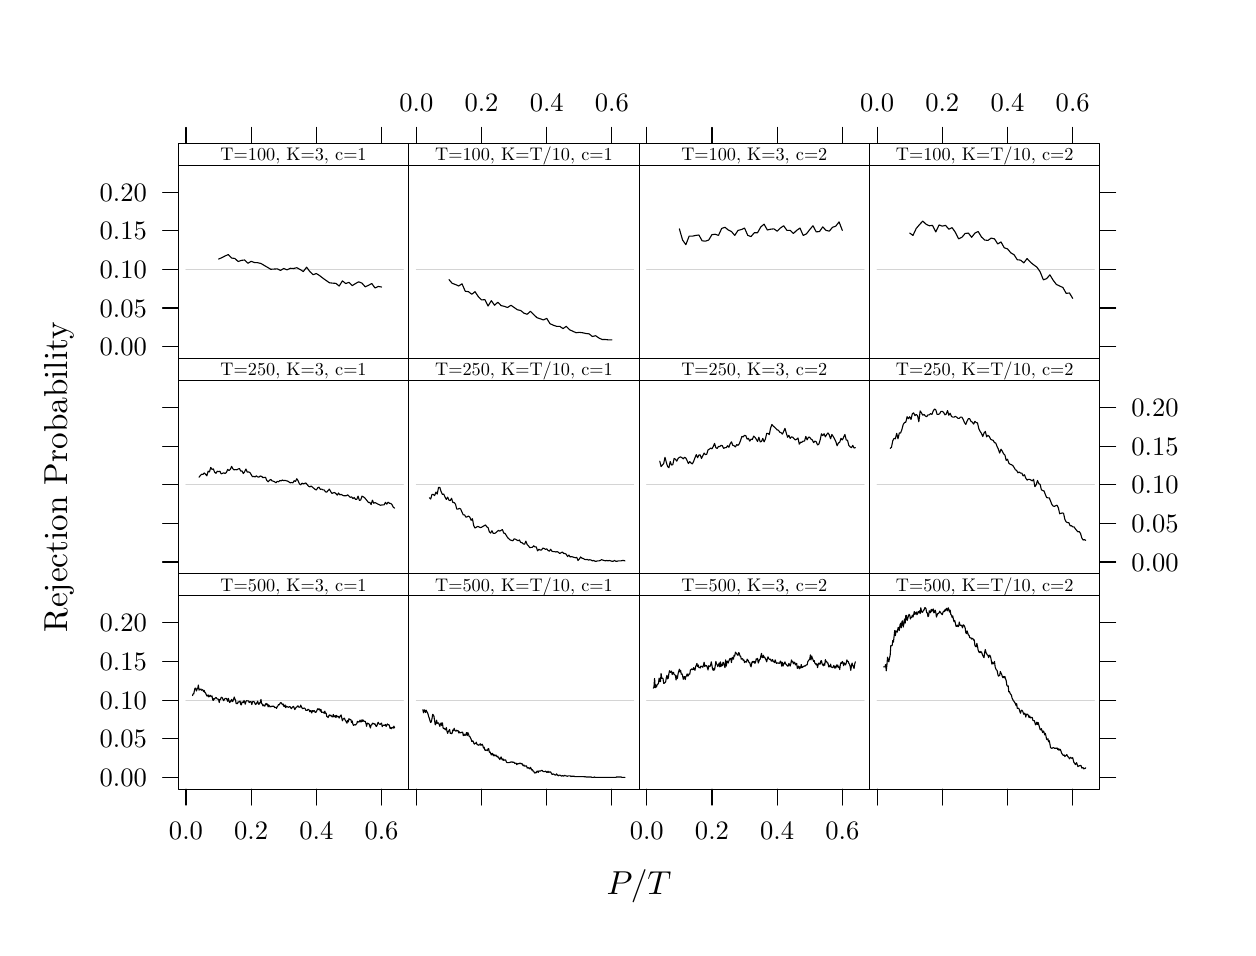
\begin{tikzpicture}[x=1pt,y=1pt]
\definecolor[named]{fillColor}{rgb}{1.00,1.00,1.00}
\path[use as bounding box,fill=fillColor,fill opacity=0.00] (0,0) rectangle (433.62,325.21);
\begin{scope}
\path[clip] (  0.00,  0.00) rectangle (433.62,325.21);

\path[] (  0.00,  0.00) rectangle (433.62,325.21);
\definecolor[named]{drawColor}{rgb}{0.00,0.00,0.00}

\node[text=drawColor,anchor=base,inner sep=0pt, outer sep=0pt, scale=  1.20] at (220.94, 12.05) {$P/T$};
\end{scope}
\begin{scope}
\path[clip] (  0.00,  0.00) rectangle (433.62,325.21);
\definecolor[named]{drawColor}{rgb}{0.00,0.00,0.00}

\node[text=drawColor,rotate= 90.00,anchor=base,inner sep=0pt, outer sep=0pt, scale=  1.20] at ( 14.29,162.76) {Rejection Probability};
\end{scope}
\begin{scope}
\path[clip] (  0.00,  0.00) rectangle (433.62,325.21);
\definecolor[named]{drawColor}{rgb}{0.00,0.00,0.00}

\path[draw=drawColor,line width= 0.4pt,line join=round,line cap=round] ( 54.44, 54.31) -- ( 48.75, 54.31);

\path[draw=drawColor,line width= 0.4pt,line join=round,line cap=round] ( 54.44, 68.27) -- ( 48.75, 68.27);

\path[draw=drawColor,line width= 0.4pt,line join=round,line cap=round] ( 54.44, 82.23) -- ( 48.75, 82.23);

\path[draw=drawColor,line width= 0.4pt,line join=round,line cap=round] ( 54.44, 96.19) -- ( 48.75, 96.19);

\path[draw=drawColor,line width= 0.4pt,line join=round,line cap=round] ( 54.44,110.15) -- ( 48.75,110.15);

\node[text=drawColor,anchor=base east,inner sep=0pt, outer sep=0pt, scale=  0.96] at ( 43.06, 51.00) {0.00};

\node[text=drawColor,anchor=base east,inner sep=0pt, outer sep=0pt, scale=  0.96] at ( 43.06, 64.96) {0.05};

\node[text=drawColor,anchor=base east,inner sep=0pt, outer sep=0pt, scale=  0.96] at ( 43.06, 78.92) {0.10};

\node[text=drawColor,anchor=base east,inner sep=0pt, outer sep=0pt, scale=  0.96] at ( 43.06, 92.88) {0.15};

\node[text=drawColor,anchor=base east,inner sep=0pt, outer sep=0pt, scale=  0.96] at ( 43.06,106.84) {0.20};
\end{scope}
\begin{scope}
\path[clip] (  0.00,  0.00) rectangle (433.62,325.21);
\definecolor[named]{drawColor}{rgb}{0.00,0.00,0.00}

\path[draw=drawColor,line width= 0.4pt,line join=round,line cap=round] ( 57.20, 50.02) -- ( 57.20, 44.32);

\path[draw=drawColor,line width= 0.4pt,line join=round,line cap=round] ( 80.76, 50.02) -- ( 80.76, 44.32);

\path[draw=drawColor,line width= 0.4pt,line join=round,line cap=round] (104.31, 50.02) -- (104.31, 44.32);

\path[draw=drawColor,line width= 0.4pt,line join=round,line cap=round] (127.87, 50.02) -- (127.87, 44.32);

\node[text=drawColor,anchor=base,inner sep=0pt, outer sep=0pt, scale=  0.96] at ( 57.20, 32.02) {0.0};

\node[text=drawColor,anchor=base,inner sep=0pt, outer sep=0pt, scale=  0.96] at ( 80.76, 32.02) {0.2};

\node[text=drawColor,anchor=base,inner sep=0pt, outer sep=0pt, scale=  0.96] at (104.31, 32.02) {0.4};

\node[text=drawColor,anchor=base,inner sep=0pt, outer sep=0pt, scale=  0.96] at (127.87, 32.02) {0.6};
\end{scope}
\begin{scope}
\path[clip] ( 54.44, 50.02) rectangle (137.69,119.88);
\definecolor[named]{drawColor}{rgb}{0.83,0.83,0.83}

\path[draw=drawColor,line width= 0.4pt,line join=round,line cap=round] ( 57.20, 82.23) --
	(135.72, 82.23);
\definecolor[named]{drawColor}{rgb}{0.00,0.00,0.00}

\path[draw=drawColor,line width= 0.4pt,line join=round,line cap=round] ( 59.56, 83.86) --
	( 59.79, 84.52) --
	( 60.03, 84.45) --
	( 60.26, 85.78) --
	( 60.50, 86.57) --
	( 60.73, 86.57) --
	( 60.97, 85.51) --
	( 61.20, 86.17) --
	( 61.44, 86.44) --
	( 61.68, 87.69) --
	( 61.91, 85.84) --
	( 62.15, 86.17) --
	( 62.38, 85.98) --
	( 62.62, 86.24) --
	( 62.85, 85.78) --
	( 63.09, 85.98) --
	( 63.32, 85.91) --
	( 63.56, 85.31) --
	( 63.80, 85.71) --
	( 64.03, 84.98) --
	( 64.27, 84.85) --
	( 64.50, 84.26) --
	( 64.74, 83.73) --
	( 64.97, 83.66) --
	( 65.21, 84.12) --
	( 65.44, 83.40) --
	( 65.68, 83.53) --
	( 65.92, 83.99) --
	( 66.15, 83.73) --
	( 66.39, 83.46) --
	( 66.62, 83.73) --
	( 66.86, 82.34) --
	( 67.09, 82.14) --
	( 67.33, 82.74) --
	( 67.56, 82.60) --
	( 67.80, 83.00) --
	( 68.04, 83.20) --
	( 68.27, 82.93) --
	( 68.51, 82.60) --
	( 68.74, 82.60) --
	( 68.98, 82.54) --
	( 69.21, 81.35) --
	( 69.45, 82.47) --
	( 69.69, 82.47) --
	( 69.92, 83.20) --
	( 70.16, 83.26) --
	( 70.39, 82.93) --
	( 70.63, 82.34) --
	( 70.86, 82.01) --
	( 71.10, 82.54) --
	( 71.33, 82.80) --
	( 71.57, 82.80) --
	( 71.81, 82.87) --
	( 72.04, 82.34) --
	( 72.28, 81.81) --
	( 72.51, 82.87) --
	( 72.75, 82.07) --
	( 72.98, 81.35) --
	( 73.22, 81.61) --
	( 73.45, 82.07) --
	( 73.69, 82.47) --
	( 73.93, 81.68) --
	( 74.16, 81.81) --
	( 74.40, 82.54) --
	( 74.63, 83.33) --
	( 74.87, 82.60) --
	( 75.10, 82.27) --
	( 75.34, 80.95) --
	( 75.57, 81.08) --
	( 75.81, 80.95) --
	( 76.05, 81.61) --
	( 76.28, 81.48) --
	( 76.52, 81.74) --
	( 76.75, 81.88) --
	( 76.99, 80.62) --
	( 77.22, 80.49) --
	( 77.46, 81.55) --
	( 77.69, 81.48) --
	( 77.93, 81.35) --
	( 78.17, 82.07) --
	( 78.40, 81.48) --
	( 78.64, 80.75) --
	( 78.87, 81.74) --
	( 79.11, 82.01) --
	( 79.34, 81.94) --
	( 79.58, 81.94) --
	( 79.81, 81.94) --
	( 80.05, 81.35) --
	( 80.29, 81.55) --
	( 80.52, 81.74) --
	( 80.76, 81.55) --
	( 80.99, 80.62) --
	( 81.23, 81.61) --
	( 81.46, 81.81) --
	( 81.70, 81.61) --
	( 81.93, 81.61) --
	( 82.17, 80.88) --
	( 82.41, 80.62) --
	( 82.64, 81.08) --
	( 82.88, 81.28) --
	( 83.11, 81.88) --
	( 83.35, 80.82) --
	( 83.58, 80.69) --
	( 83.82, 81.28) --
	( 84.05, 81.21) --
	( 84.29, 82.47) --
	( 84.53, 80.95) --
	( 84.76, 80.82) --
	( 85.00, 80.16) --
	( 85.23, 80.49) --
	( 85.47, 80.16) --
	( 85.70, 80.02) --
	( 85.94, 80.75) --
	( 86.17, 81.02) --
	( 86.41, 80.55) --
	( 86.65, 80.82) --
	( 86.88, 79.76) --
	( 87.12, 80.49) --
	( 87.35, 80.09) --
	( 87.59, 79.76) --
	( 87.82, 80.02) --
	( 88.06, 79.83) --
	( 88.29, 80.02) --
	( 88.53, 80.02) --
	( 88.77, 80.02) --
	( 89.00, 79.96) --
	( 89.24, 79.50) --
	( 89.47, 79.56) --
	( 89.71, 79.63) --
	( 89.94, 79.23) --
	( 90.18, 79.83) --
	( 90.41, 80.09) --
	( 90.65, 80.62) --
	( 90.89, 80.49) --
	( 91.12, 80.88) --
	( 91.36, 81.28) --
	( 91.59, 81.28) --
	( 91.83, 80.95) --
	( 92.06, 80.62) --
	( 92.30, 80.82) --
	( 92.53, 80.02) --
	( 92.77, 79.89) --
	( 93.01, 80.49) --
	( 93.24, 79.50) --
	( 93.48, 80.02) --
	( 93.71, 79.89) --
	( 93.95, 79.76) --
	( 94.18, 79.63) --
	( 94.42, 79.76) --
	( 94.66, 79.89) --
	( 94.89, 79.76) --
	( 95.13, 79.30) --
	( 95.36, 79.17) --
	( 95.60, 79.63) --
	( 95.83, 79.83) --
	( 96.07, 79.96) --
	( 96.30, 79.36) --
	( 96.54, 78.83) --
	( 96.78, 79.23) --
	( 97.01, 79.63) --
	( 97.25, 79.69) --
	( 97.48, 80.09) --
	( 97.72, 80.16) --
	( 97.95, 79.69) --
	( 98.19, 79.69) --
	( 98.42, 79.63) --
	( 98.66, 80.42) --
	( 98.90, 79.83) --
	( 99.13, 79.43) --
	( 99.37, 79.10) --
	( 99.60, 79.23) --
	( 99.84, 79.36) --
	(100.07, 79.30) --
	(100.31, 79.03) --
	(100.54, 78.50) --
	(100.78, 78.50) --
	(101.02, 78.50) --
	(101.25, 78.90) --
	(101.49, 78.90) --
	(101.72, 78.57) --
	(101.96, 77.98) --
	(102.19, 78.44) --
	(102.43, 78.31) --
	(102.66, 77.58) --
	(102.90, 78.44) --
	(103.14, 78.11) --
	(103.37, 78.44) --
	(103.61, 78.44) --
	(103.84, 77.84) --
	(104.08, 77.78) --
	(104.31, 77.98) --
	(104.55, 78.57) --
	(104.78, 79.10) --
	(105.02, 78.77) --
	(105.26, 79.10) --
	(105.49, 78.97) --
	(105.73, 78.24) --
	(105.96, 78.90) --
	(106.20, 77.78) --
	(106.43, 77.91) --
	(106.67, 77.84) --
	(106.90, 77.84) --
	(107.14, 77.45) --
	(107.38, 78.24) --
	(107.61, 77.45) --
	(107.85, 77.51) --
	(108.08, 76.32) --
	(108.32, 76.19) --
	(108.55, 75.93) --
	(108.79, 76.52) --
	(109.02, 76.85) --
	(109.26, 76.52) --
	(109.50, 76.79) --
	(109.73, 76.52) --
	(109.97, 76.19) --
	(110.20, 76.19) --
	(110.44, 77.05) --
	(110.67, 76.19) --
	(110.91, 76.32) --
	(111.14, 76.65) --
	(111.38, 75.93) --
	(111.62, 76.72) --
	(111.85, 76.19) --
	(112.09, 76.39) --
	(112.32, 76.26) --
	(112.56, 75.73) --
	(112.79, 76.19) --
	(113.03, 76.65) --
	(113.26, 76.85) --
	(113.50, 75.73) --
	(113.74, 74.74) --
	(113.97, 75.40) --
	(114.21, 75.53) --
	(114.44, 75.73) --
	(114.68, 75.07) --
	(114.91, 74.80) --
	(115.15, 74.27) --
	(115.38, 73.88) --
	(115.62, 74.87) --
	(115.86, 74.34) --
	(116.09, 75.53) --
	(116.33, 75.13) --
	(116.56, 75.26) --
	(116.80, 75.13) --
	(117.03, 74.14) --
	(117.27, 74.67) --
	(117.51, 73.55) --
	(117.74, 73.08) --
	(117.98, 73.28) --
	(118.21, 73.35) --
	(118.45, 73.21) --
	(118.68, 73.48) --
	(118.92, 73.74) --
	(119.15, 74.54) --
	(119.39, 74.27) --
	(119.63, 74.40) --
	(119.86, 74.34) --
	(120.10, 75.00) --
	(120.33, 74.34) --
	(120.57, 74.34) --
	(120.80, 75.13) --
	(121.04, 74.54) --
	(121.27, 75.00) --
	(121.51, 74.60) --
	(121.75, 74.54) --
	(121.98, 74.54) --
	(122.22, 73.88) --
	(122.45, 72.75) --
	(122.69, 73.88) --
	(122.92, 73.88) --
	(123.16, 73.68) --
	(123.39, 73.61) --
	(123.63, 72.75) --
	(123.87, 72.16) --
	(124.10, 73.28) --
	(124.34, 73.28) --
	(124.57, 73.88) --
	(124.81, 73.68) --
	(125.04, 73.81) --
	(125.28, 73.48) --
	(125.51, 73.61) --
	(125.75, 73.02) --
	(125.99, 72.69) --
	(126.22, 73.02) --
	(126.46, 73.88) --
	(126.69, 74.21) --
	(126.93, 73.61) --
	(127.16, 73.55) --
	(127.40, 73.41) --
	(127.63, 73.74) --
	(127.87, 73.94) --
	(128.11, 72.62) --
	(128.34, 73.08) --
	(128.58, 73.15) --
	(128.81, 73.15) --
	(129.05, 73.08) --
	(129.28, 73.41) --
	(129.52, 72.69) --
	(129.75, 73.15) --
	(129.99, 73.61) --
	(130.23, 73.28) --
	(130.46, 73.41) --
	(130.70, 73.02) --
	(130.93, 72.02) --
	(131.17, 72.36) --
	(131.40, 71.89) --
	(131.64, 72.29) --
	(131.87, 72.36) --
	(132.11, 72.09) --
	(132.35, 72.82) --
	(132.58, 72.16);
\end{scope}
\begin{scope}
\path[clip] (  0.00,  0.00) rectangle (433.62,325.21);
\definecolor[named]{drawColor}{rgb}{0.00,0.00,0.00}

\path[draw=drawColor,line width= 0.4pt,line join=round,line cap=round] ( 54.44, 50.02) rectangle (137.69,119.88);
\end{scope}
\begin{scope}
\path[clip] ( 54.44,119.88) rectangle (137.69,127.83);

\path[] ( 54.44,119.88) rectangle (137.69,127.83);
\definecolor[named]{drawColor}{rgb}{0.00,0.00,0.00}

\node[text=drawColor,anchor=base west,inner sep=0pt, outer sep=0pt, scale=  0.66] at ( 69.67,121.58) {T=500, K=3, c=1};
\end{scope}
\begin{scope}
\path[clip] (  0.00,  0.00) rectangle (433.62,325.21);
\definecolor[named]{drawColor}{rgb}{0.00,0.00,0.00}

\path[draw=drawColor,line width= 0.4pt,line join=round,line cap=round] ( 54.44,119.88) rectangle (137.69,127.83);
\end{scope}
\begin{scope}
\path[clip] (  0.00,  0.00) rectangle (433.62,325.21);
\definecolor[named]{drawColor}{rgb}{0.00,0.00,0.00}

\path[draw=drawColor,line width= 0.4pt,line join=round,line cap=round] (140.45, 50.02) -- (140.45, 44.32);

\path[draw=drawColor,line width= 0.4pt,line join=round,line cap=round] (164.01, 50.02) -- (164.01, 44.32);

\path[draw=drawColor,line width= 0.4pt,line join=round,line cap=round] (187.56, 50.02) -- (187.56, 44.32);

\path[draw=drawColor,line width= 0.4pt,line join=round,line cap=round] (211.12, 50.02) -- (211.12, 44.32);
\end{scope}
\begin{scope}
\path[clip] (137.69, 50.02) rectangle (220.94,119.88);
\definecolor[named]{drawColor}{rgb}{0.83,0.83,0.83}

\path[draw=drawColor,line width= 0.4pt,line join=round,line cap=round] (140.45, 82.23) --
	(218.97, 82.23);
\definecolor[named]{drawColor}{rgb}{0.00,0.00,0.00}

\path[draw=drawColor,line width= 0.4pt,line join=round,line cap=round] (142.80, 78.74) --
	(143.04, 77.62) --
	(143.28, 78.74) --
	(143.51, 78.46) --
	(143.75, 77.76) --
	(143.98, 78.60) --
	(144.22, 78.04) --
	(144.45, 77.76) --
	(144.69, 77.06) --
	(144.92, 76.22) --
	(145.16, 75.53) --
	(145.40, 74.69) --
	(145.63, 74.13) --
	(145.87, 74.41) --
	(146.10, 75.53) --
	(146.34, 77.06) --
	(146.57, 76.92) --
	(146.81, 76.36) --
	(147.05, 74.69) --
	(147.28, 73.29) --
	(147.52, 73.71) --
	(147.75, 74.97) --
	(147.99, 73.85) --
	(148.22, 73.99) --
	(148.46, 73.99) --
	(148.69, 73.43) --
	(148.93, 72.73) --
	(149.17, 73.57) --
	(149.40, 73.99) --
	(149.64, 73.01) --
	(149.87, 73.99) --
	(150.11, 72.17) --
	(150.34, 71.90) --
	(150.58, 72.04) --
	(150.81, 71.62) --
	(151.05, 71.48) --
	(151.29, 72.31) --
	(151.52, 70.92) --
	(151.76, 70.22) --
	(151.99, 70.92) --
	(152.23, 71.20) --
	(152.46, 71.62) --
	(152.70, 70.22) --
	(152.93, 70.36) --
	(153.17, 70.08) --
	(153.41, 70.36) --
	(153.64, 71.48) --
	(153.88, 71.20) --
	(154.11, 72.04) --
	(154.35, 71.34) --
	(154.58, 71.06) --
	(154.82, 71.06) --
	(155.05, 71.34) --
	(155.29, 71.06) --
	(155.53, 71.20) --
	(155.76, 70.36) --
	(156.00, 70.78) --
	(156.23, 70.36) --
	(156.47, 70.50) --
	(156.70, 70.50) --
	(156.94, 70.64) --
	(157.17, 70.64) --
	(157.41, 69.38) --
	(157.65, 69.94) --
	(157.88, 69.52) --
	(158.12, 69.52) --
	(158.35, 69.80) --
	(158.59, 70.50) --
	(158.82, 69.38) --
	(159.06, 70.50) --
	(159.29, 69.94) --
	(159.53, 69.10) --
	(159.77, 69.10) --
	(160.00, 68.55) --
	(160.24, 68.13) --
	(160.47, 67.29) --
	(160.71, 67.43) --
	(160.94, 67.43) --
	(161.18, 66.73) --
	(161.41, 66.31) --
	(161.65, 66.59) --
	(161.89, 66.59) --
	(162.12, 67.01) --
	(162.36, 66.17) --
	(162.59, 66.17) --
	(162.83, 65.89) --
	(163.06, 66.03) --
	(163.30, 66.03) --
	(163.53, 66.45) --
	(163.77, 65.89) --
	(164.01, 66.03) --
	(164.24, 66.31) --
	(164.48, 65.75) --
	(164.71, 64.92) --
	(164.95, 65.19) --
	(165.18, 64.22) --
	(165.42, 64.08) --
	(165.65, 64.22) --
	(165.89, 64.08) --
	(166.13, 63.94) --
	(166.36, 64.64) --
	(166.60, 64.64) --
	(166.83, 63.38) --
	(167.07, 63.52) --
	(167.30, 62.96) --
	(167.54, 62.40) --
	(167.77, 62.96) --
	(168.01, 62.96) --
	(168.25, 62.12) --
	(168.48, 62.54) --
	(168.72, 62.12) --
	(168.95, 62.12) --
	(169.19, 62.40) --
	(169.42, 61.98) --
	(169.66, 61.70) --
	(169.90, 61.98) --
	(170.13, 61.29) --
	(170.37, 61.29) --
	(170.60, 60.73) --
	(170.84, 61.29) --
	(171.07, 61.70) --
	(171.31, 61.01) --
	(171.54, 60.59) --
	(171.78, 61.01) --
	(172.02, 60.45) --
	(172.25, 60.59) --
	(172.49, 60.59) --
	(172.72, 60.59) --
	(172.96, 59.89) --
	(173.19, 59.61) --
	(173.43, 59.61) --
	(173.66, 59.61) --
	(173.90, 59.61) --
	(174.14, 59.75) --
	(174.37, 59.75) --
	(174.61, 59.89) --
	(174.84, 59.89) --
	(175.08, 59.75) --
	(175.31, 59.89) --
	(175.55, 59.75) --
	(175.78, 59.75) --
	(176.02, 59.33) --
	(176.26, 59.47) --
	(176.49, 59.47) --
	(176.73, 58.91) --
	(176.96, 59.19) --
	(177.20, 59.33) --
	(177.43, 59.19) --
	(177.67, 59.33) --
	(177.90, 59.47) --
	(178.14, 59.33) --
	(178.38, 59.19) --
	(178.61, 59.33) --
	(178.85, 58.77) --
	(179.08, 58.49) --
	(179.32, 58.77) --
	(179.55, 58.35) --
	(179.79, 58.49) --
	(180.02, 58.35) --
	(180.26, 58.49) --
	(180.50, 57.66) --
	(180.73, 57.80) --
	(180.97, 57.80) --
	(181.20, 57.52) --
	(181.44, 57.38) --
	(181.67, 57.94) --
	(181.91, 57.52) --
	(182.14, 56.96) --
	(182.38, 57.10) --
	(182.62, 56.54) --
	(182.85, 56.54) --
	(183.09, 55.98) --
	(183.32, 55.84) --
	(183.56, 56.12) --
	(183.79, 55.98) --
	(184.03, 56.54) --
	(184.26, 56.54) --
	(184.50, 56.12) --
	(184.74, 56.68) --
	(184.97, 56.54) --
	(185.21, 56.54) --
	(185.44, 56.68) --
	(185.68, 56.82) --
	(185.91, 56.82) --
	(186.15, 56.54) --
	(186.38, 56.40) --
	(186.62, 56.40) --
	(186.86, 56.40) --
	(187.09, 56.54) --
	(187.33, 56.40) --
	(187.56, 56.12) --
	(187.80, 56.12) --
	(188.03, 56.54) --
	(188.27, 56.12) --
	(188.50, 56.26) --
	(188.74, 56.26) --
	(188.98, 56.26) --
	(189.21, 55.84) --
	(189.45, 55.42) --
	(189.68, 55.42) --
	(189.92, 55.56) --
	(190.15, 55.42) --
	(190.39, 55.28) --
	(190.62, 55.14) --
	(190.86, 55.14) --
	(191.10, 55.56) --
	(191.33, 55.28) --
	(191.57, 55.00) --
	(191.80, 54.86) --
	(192.04, 55.14) --
	(192.27, 55.14) --
	(192.51, 55.00) --
	(192.74, 54.86) --
	(192.98, 54.72) --
	(193.22, 55.00) --
	(193.45, 54.86) --
	(193.69, 54.72) --
	(193.92, 55.00) --
	(194.16, 55.00) --
	(194.39, 54.86) --
	(194.63, 54.86) --
	(194.87, 54.72) --
	(195.10, 54.72) --
	(195.34, 54.86) --
	(195.57, 54.86) --
	(195.81, 54.86) --
	(196.04, 54.86) --
	(196.28, 54.58) --
	(196.51, 54.72) --
	(196.75, 54.72) --
	(196.99, 54.72) --
	(197.22, 54.72) --
	(197.46, 54.72) --
	(197.69, 54.58) --
	(197.93, 54.58) --
	(198.16, 54.58) --
	(198.40, 54.58) --
	(198.63, 54.58) --
	(198.87, 54.58) --
	(199.11, 54.58) --
	(199.34, 54.58) --
	(199.58, 54.58) --
	(199.81, 54.58) --
	(200.05, 54.58) --
	(200.28, 54.58) --
	(200.52, 54.58) --
	(200.75, 54.58) --
	(200.99, 54.58) --
	(201.23, 54.45) --
	(201.46, 54.58) --
	(201.70, 54.45) --
	(201.93, 54.45) --
	(202.17, 54.45) --
	(202.40, 54.45) --
	(202.64, 54.45) --
	(202.87, 54.45) --
	(203.11, 54.45) --
	(203.35, 54.45) --
	(203.58, 54.45) --
	(203.82, 54.31) --
	(204.05, 54.31) --
	(204.29, 54.31) --
	(204.52, 54.31) --
	(204.76, 54.45) --
	(204.99, 54.31) --
	(205.23, 54.31) --
	(205.47, 54.31) --
	(205.70, 54.31) --
	(205.94, 54.31) --
	(206.17, 54.31) --
	(206.41, 54.31) --
	(206.64, 54.31) --
	(206.88, 54.31) --
	(207.11, 54.31) --
	(207.35, 54.31) --
	(207.59, 54.31) --
	(207.82, 54.31) --
	(208.06, 54.31) --
	(208.29, 54.31) --
	(208.53, 54.31) --
	(208.76, 54.31) --
	(209.00, 54.31) --
	(209.23, 54.31) --
	(209.47, 54.31) --
	(209.71, 54.31) --
	(209.94, 54.31) --
	(210.18, 54.31) --
	(210.41, 54.31) --
	(210.65, 54.31) --
	(210.88, 54.31) --
	(211.12, 54.31) --
	(211.35, 54.31) --
	(211.59, 54.31) --
	(211.83, 54.31) --
	(212.06, 54.31) --
	(212.30, 54.31) --
	(212.53, 54.31) --
	(212.77, 54.45) --
	(213.00, 54.45) --
	(213.24, 54.45) --
	(213.47, 54.45) --
	(213.71, 54.45) --
	(213.95, 54.45) --
	(214.18, 54.45) --
	(214.42, 54.45) --
	(214.65, 54.31) --
	(214.89, 54.31) --
	(215.12, 54.31) --
	(215.36, 54.31) --
	(215.59, 54.31) --
	(215.83, 54.31);
\end{scope}
\begin{scope}
\path[clip] (  0.00,  0.00) rectangle (433.62,325.21);
\definecolor[named]{drawColor}{rgb}{0.00,0.00,0.00}

\path[draw=drawColor,line width= 0.4pt,line join=round,line cap=round] (137.69, 50.02) rectangle (220.94,119.88);
\end{scope}
\begin{scope}
\path[clip] (137.69,119.88) rectangle (220.94,127.83);

\path[] (137.69,119.88) rectangle (220.94,127.83);
\definecolor[named]{drawColor}{rgb}{0.00,0.00,0.00}

\node[text=drawColor,anchor=base west,inner sep=0pt, outer sep=0pt, scale=  0.66] at (147.24,121.58) {T=500, K=T/10, c=1};
\end{scope}
\begin{scope}
\path[clip] (  0.00,  0.00) rectangle (433.62,325.21);
\definecolor[named]{drawColor}{rgb}{0.00,0.00,0.00}

\path[draw=drawColor,line width= 0.4pt,line join=round,line cap=round] (137.69,119.88) rectangle (220.94,127.83);
\end{scope}
\begin{scope}
\path[clip] (  0.00,  0.00) rectangle (433.62,325.21);
\definecolor[named]{drawColor}{rgb}{0.00,0.00,0.00}

\path[draw=drawColor,line width= 0.4pt,line join=round,line cap=round] (223.70, 50.02) -- (223.70, 44.32);

\path[draw=drawColor,line width= 0.4pt,line join=round,line cap=round] (247.26, 50.02) -- (247.26, 44.32);

\path[draw=drawColor,line width= 0.4pt,line join=round,line cap=round] (270.81, 50.02) -- (270.81, 44.32);

\path[draw=drawColor,line width= 0.4pt,line join=round,line cap=round] (294.37, 50.02) -- (294.37, 44.32);

\node[text=drawColor,anchor=base,inner sep=0pt, outer sep=0pt, scale=  0.96] at (223.70, 32.02) {0.0};

\node[text=drawColor,anchor=base,inner sep=0pt, outer sep=0pt, scale=  0.96] at (247.26, 32.02) {0.2};

\node[text=drawColor,anchor=base,inner sep=0pt, outer sep=0pt, scale=  0.96] at (270.81, 32.02) {0.4};

\node[text=drawColor,anchor=base,inner sep=0pt, outer sep=0pt, scale=  0.96] at (294.37, 32.02) {0.6};
\end{scope}
\begin{scope}
\path[clip] (220.94, 50.02) rectangle (304.19,119.88);
\definecolor[named]{drawColor}{rgb}{0.83,0.83,0.83}

\path[draw=drawColor,line width= 0.4pt,line join=round,line cap=round] (223.70, 82.23) --
	(302.22, 82.23);
\definecolor[named]{drawColor}{rgb}{0.00,0.00,0.00}

\path[draw=drawColor,line width= 0.4pt,line join=round,line cap=round] (226.05, 86.55) --
	(226.29, 86.83) --
	(226.53, 90.04) --
	(226.76, 86.69) --
	(227.00, 87.67) --
	(227.23, 86.97) --
	(227.47, 87.81) --
	(227.70, 87.95) --
	(227.94, 88.37) --
	(228.17, 90.18) --
	(228.41, 88.93) --
	(228.65, 88.93) --
	(228.88, 91.86) --
	(229.12, 90.04) --
	(229.35, 90.18) --
	(229.59, 90.04) --
	(229.82, 88.23) --
	(230.06, 88.37) --
	(230.29, 88.51) --
	(230.53, 88.79) --
	(230.77, 90.32) --
	(231.00, 91.16) --
	(231.24, 89.90) --
	(231.47, 90.18) --
	(231.71, 91.86) --
	(231.94, 92.84) --
	(232.18, 92.28) --
	(232.41, 92.28) --
	(232.65, 92.70) --
	(232.89, 91.44) --
	(233.12, 92.14) --
	(233.36, 92.28) --
	(233.59, 91.44) --
	(233.83, 91.44) --
	(234.06, 91.02) --
	(234.30, 89.49) --
	(234.53, 91.02) --
	(234.77, 90.04) --
	(235.01, 91.72) --
	(235.24, 92.56) --
	(235.48, 93.39) --
	(235.71, 92.42) --
	(235.95, 92.98) --
	(236.18, 91.58) --
	(236.42, 91.72) --
	(236.65, 91.02) --
	(236.89, 89.77) --
	(237.13, 90.60) --
	(237.36, 90.74) --
	(237.60, 89.63) --
	(237.83, 90.74) --
	(238.07, 91.02) --
	(238.30, 91.72) --
	(238.54, 90.88) --
	(238.77, 91.16) --
	(239.01, 91.72) --
	(239.25, 91.58) --
	(239.48, 93.12) --
	(239.72, 93.26) --
	(239.95, 93.53) --
	(240.19, 93.26) --
	(240.42, 93.26) --
	(240.66, 93.95) --
	(240.89, 93.39) --
	(241.13, 92.98) --
	(241.37, 94.37) --
	(241.60, 94.79) --
	(241.84, 95.49) --
	(242.07, 94.37) --
	(242.31, 94.93) --
	(242.54, 93.95) --
	(242.78, 94.09) --
	(243.01, 93.81) --
	(243.25, 94.51) --
	(243.49, 94.37) --
	(243.72, 94.37) --
	(243.96, 94.09) --
	(244.19, 94.79) --
	(244.43, 95.91) --
	(244.66, 94.37) --
	(244.90, 94.79) --
	(245.13, 94.65) --
	(245.37, 94.65) --
	(245.61, 93.95) --
	(245.84, 93.12) --
	(246.08, 94.65) --
	(246.31, 94.37) --
	(246.55, 94.37) --
	(246.78, 94.93) --
	(247.02, 96.05) --
	(247.26, 94.79) --
	(247.49, 93.39) --
	(247.73, 92.98) --
	(247.96, 93.67) --
	(248.20, 93.12) --
	(248.43, 94.51) --
	(248.67, 96.19) --
	(248.90, 95.35) --
	(249.14, 95.07) --
	(249.38, 94.37) --
	(249.61, 94.79) --
	(249.85, 95.63) --
	(250.08, 94.23) --
	(250.32, 96.05) --
	(250.55, 94.37) --
	(250.79, 95.21) --
	(251.02, 94.65) --
	(251.26, 95.91) --
	(251.50, 95.63) --
	(251.73, 94.79) --
	(251.97, 93.95) --
	(252.20, 96.75) --
	(252.44, 94.51) --
	(252.67, 96.19) --
	(252.91, 96.33) --
	(253.14, 95.63) --
	(253.38, 96.33) --
	(253.62, 97.02) --
	(253.85, 97.30) --
	(254.09, 97.16) --
	(254.32, 95.77) --
	(254.56, 97.72) --
	(254.79, 97.16) --
	(255.03, 97.02) --
	(255.26, 98.42) --
	(255.50, 98.14) --
	(255.74, 99.54) --
	(255.97, 99.26) --
	(256.21, 98.98) --
	(256.44, 98.56) --
	(256.68, 98.42) --
	(256.91, 99.40) --
	(257.15, 99.12) --
	(257.38, 98.14) --
	(257.62, 98.14) --
	(257.86, 97.02) --
	(258.09, 97.16) --
	(258.33, 97.16) --
	(258.56, 96.61) --
	(258.80, 96.75) --
	(259.03, 95.77) --
	(259.27, 96.19) --
	(259.50, 96.05) --
	(259.74, 95.91) --
	(259.98, 97.02) --
	(260.21, 96.75) --
	(260.45, 96.33) --
	(260.68, 95.77) --
	(260.92, 95.77) --
	(261.15, 94.79) --
	(261.39, 94.23) --
	(261.62, 95.49) --
	(261.86, 96.19) --
	(262.10, 95.77) --
	(262.33, 96.19) --
	(262.57, 96.19) --
	(262.80, 95.49) --
	(263.04, 96.05) --
	(263.27, 97.16) --
	(263.51, 96.88) --
	(263.74, 97.30) --
	(263.98, 95.63) --
	(264.22, 96.19) --
	(264.45, 96.88) --
	(264.69, 97.02) --
	(264.92, 98.14) --
	(265.16, 99.12) --
	(265.39, 97.58) --
	(265.63, 97.58) --
	(265.86, 98.42) --
	(266.10, 97.58) --
	(266.34, 97.72) --
	(266.57, 97.16) --
	(266.81, 96.75) --
	(267.04, 96.05) --
	(267.28, 97.16) --
	(267.51, 97.86) --
	(267.75, 97.30) --
	(267.98, 97.02) --
	(268.22, 96.88) --
	(268.46, 97.02) --
	(268.69, 96.33) --
	(268.93, 96.33) --
	(269.16, 96.88) --
	(269.40, 96.19) --
	(269.63, 96.19) --
	(269.87, 95.77) --
	(270.11, 96.75) --
	(270.34, 96.05) --
	(270.58, 95.49) --
	(270.81, 95.63) --
	(271.05, 95.63) --
	(271.28, 95.63) --
	(271.52, 95.49) --
	(271.75, 95.63) --
	(271.99, 96.33) --
	(272.23, 95.91) --
	(272.46, 94.51) --
	(272.70, 95.91) --
	(272.93, 94.51) --
	(273.17, 95.21) --
	(273.40, 95.49) --
	(273.64, 96.05) --
	(273.87, 95.21) --
	(274.11, 95.21) --
	(274.35, 94.79) --
	(274.58, 94.51) --
	(274.82, 94.51) --
	(275.05, 95.49) --
	(275.29, 95.07) --
	(275.52, 94.51) --
	(275.76, 95.35) --
	(275.99, 96.75) --
	(276.23, 96.05) --
	(276.47, 96.19) --
	(276.70, 95.35) --
	(276.94, 95.77) --
	(277.17, 95.91) --
	(277.41, 94.93) --
	(277.64, 95.21) --
	(277.88, 95.49) --
	(278.11, 93.67) --
	(278.35, 94.23) --
	(278.59, 94.51) --
	(278.82, 93.53) --
	(279.06, 94.23) --
	(279.29, 93.81) --
	(279.53, 95.07) --
	(279.76, 93.95) --
	(280.00, 94.09) --
	(280.23, 94.37) --
	(280.47, 94.37) --
	(280.71, 94.65) --
	(280.94, 94.51) --
	(281.18, 94.79) --
	(281.41, 94.93) --
	(281.65, 94.93) --
	(281.88, 96.05) --
	(282.12, 96.47) --
	(282.35, 96.75) --
	(282.59, 97.02) --
	(282.83, 98.56) --
	(283.06, 96.75) --
	(283.30, 98.14) --
	(283.53, 97.44) --
	(283.77, 96.88) --
	(284.00, 96.19) --
	(284.24, 96.47) --
	(284.47, 95.49) --
	(284.71, 95.35) --
	(284.95, 94.93) --
	(285.18, 95.35) --
	(285.42, 93.95) --
	(285.65, 95.07) --
	(285.89, 95.63) --
	(286.12, 95.21) --
	(286.36, 95.21) --
	(286.59, 96.33) --
	(286.83, 96.47) --
	(287.07, 95.35) --
	(287.30, 94.93) --
	(287.54, 94.65) --
	(287.77, 95.35) --
	(288.01, 94.79) --
	(288.24, 96.88) --
	(288.48, 96.05) --
	(288.71, 96.19) --
	(288.95, 95.63) --
	(289.19, 95.63) --
	(289.42, 94.23) --
	(289.66, 94.65) --
	(289.89, 94.23) --
	(290.13, 95.21) --
	(290.36, 94.23) --
	(290.60, 94.09) --
	(290.83, 93.95) --
	(291.07, 94.23) --
	(291.31, 94.79) --
	(291.54, 93.81) --
	(291.78, 94.37) --
	(292.01, 93.81) --
	(292.25, 94.93) --
	(292.48, 94.23) --
	(292.72, 94.93) --
	(292.96, 94.09) --
	(293.19, 94.23) --
	(293.43, 93.26) --
	(293.66, 95.07) --
	(293.90, 95.77) --
	(294.13, 95.49) --
	(294.37, 96.19) --
	(294.60, 95.77) --
	(294.84, 94.65) --
	(295.08, 95.63) --
	(295.31, 95.35) --
	(295.55, 94.93) --
	(295.78, 95.63) --
	(296.02, 96.75) --
	(296.25, 96.19) --
	(296.49, 96.19) --
	(296.72, 95.49) --
	(296.96, 95.21) --
	(297.20, 94.37) --
	(297.43, 92.98) --
	(297.67, 94.65) --
	(297.90, 95.63) --
	(298.14, 94.79) --
	(298.37, 94.23) --
	(298.61, 93.67) --
	(298.84, 95.21) --
	(299.08, 96.05);
\end{scope}
\begin{scope}
\path[clip] (  0.00,  0.00) rectangle (433.62,325.21);
\definecolor[named]{drawColor}{rgb}{0.00,0.00,0.00}

\path[draw=drawColor,line width= 0.4pt,line join=round,line cap=round] (220.94, 50.02) rectangle (304.19,119.88);
\end{scope}
\begin{scope}
\path[clip] (220.94,119.88) rectangle (304.19,127.83);

\path[] (220.94,119.88) rectangle (304.19,127.83);
\definecolor[named]{drawColor}{rgb}{0.00,0.00,0.00}

\node[text=drawColor,anchor=base west,inner sep=0pt, outer sep=0pt, scale=  0.66] at (236.17,121.58) {T=500, K=3, c=2};
\end{scope}
\begin{scope}
\path[clip] (  0.00,  0.00) rectangle (433.62,325.21);
\definecolor[named]{drawColor}{rgb}{0.00,0.00,0.00}

\path[draw=drawColor,line width= 0.4pt,line join=round,line cap=round] (220.94,119.88) rectangle (304.19,127.83);
\end{scope}
\begin{scope}
\path[clip] (  0.00,  0.00) rectangle (433.62,325.21);
\definecolor[named]{drawColor}{rgb}{0.00,0.00,0.00}

\path[draw=drawColor,line width= 0.4pt,line join=round,line cap=round] (306.95, 50.02) -- (306.95, 44.32);

\path[draw=drawColor,line width= 0.4pt,line join=round,line cap=round] (330.50, 50.02) -- (330.50, 44.32);

\path[draw=drawColor,line width= 0.4pt,line join=round,line cap=round] (354.06, 50.02) -- (354.06, 44.32);

\path[draw=drawColor,line width= 0.4pt,line join=round,line cap=round] (377.62, 50.02) -- (377.62, 44.32);

\path[draw=drawColor,line width= 0.4pt,line join=round,line cap=round] (387.44, 54.31) -- (393.13, 54.31);

\path[draw=drawColor,line width= 0.4pt,line join=round,line cap=round] (387.44, 68.27) -- (393.13, 68.27);

\path[draw=drawColor,line width= 0.4pt,line join=round,line cap=round] (387.44, 82.23) -- (393.13, 82.23);

\path[draw=drawColor,line width= 0.4pt,line join=round,line cap=round] (387.44, 96.19) -- (393.13, 96.19);

\path[draw=drawColor,line width= 0.4pt,line join=round,line cap=round] (387.44,110.15) -- (393.13,110.15);
\end{scope}
\begin{scope}
\path[clip] (304.19, 50.02) rectangle (387.44,119.88);
\definecolor[named]{drawColor}{rgb}{0.83,0.83,0.83}

\path[draw=drawColor,line width= 0.4pt,line join=round,line cap=round] (306.95, 82.23) --
	(385.47, 82.23);
\definecolor[named]{drawColor}{rgb}{0.00,0.00,0.00}

\path[draw=drawColor,line width= 0.4pt,line join=round,line cap=round] (309.30, 94.23) --
	(309.54, 94.23) --
	(309.77, 94.23) --
	(310.01, 95.07) --
	(310.25, 92.84) --
	(310.48, 94.93) --
	(310.72, 97.72) --
	(310.95, 96.61) --
	(311.19, 96.05) --
	(311.42, 97.44) --
	(311.66, 98.42) --
	(311.89,101.91) --
	(312.13,101.91) --
	(312.37,101.91) --
	(312.60,103.73) --
	(312.84,103.17) --
	(313.07,105.26) --
	(313.31,107.36) --
	(313.54,105.54) --
	(313.78,107.22) --
	(314.01,107.08) --
	(314.25,106.80) --
	(314.49,108.33) --
	(314.72,108.47) --
	(314.96,107.36) --
	(315.19,109.31) --
	(315.43,110.01) --
	(315.66,108.33) --
	(315.90,110.57) --
	(316.13,110.85) --
	(316.37,108.61) --
	(316.61,109.73) --
	(316.84,111.54) --
	(317.08,110.01) --
	(317.31,112.80) --
	(317.55,112.80) --
	(317.78,110.99) --
	(318.02,111.68) --
	(318.25,112.66) --
	(318.49,113.22) --
	(318.73,112.94) --
	(318.96,111.54) --
	(319.20,112.10) --
	(319.43,112.10) --
	(319.67,112.94) --
	(319.90,112.24) --
	(320.14,113.08) --
	(320.37,114.20) --
	(320.61,113.22) --
	(320.85,113.50) --
	(321.08,114.06) --
	(321.32,113.08) --
	(321.55,113.50) --
	(321.79,114.20) --
	(322.02,113.78) --
	(322.26,114.48) --
	(322.50,113.50) --
	(322.73,115.59) --
	(322.97,114.34) --
	(323.20,113.92) --
	(323.44,114.06) --
	(323.67,114.75) --
	(323.91,114.75) --
	(324.14,115.59) --
	(324.38,115.59) --
	(324.62,115.17) --
	(324.85,113.78) --
	(325.09,113.78) --
	(325.32,112.38) --
	(325.56,112.66) --
	(325.79,114.48) --
	(326.03,114.34) --
	(326.26,113.78) --
	(326.50,115.03) --
	(326.74,114.34) --
	(326.97,114.75) --
	(327.21,115.17) --
	(327.44,113.78) --
	(327.68,113.92) --
	(327.91,114.75) --
	(328.15,113.92) --
	(328.38,112.24) --
	(328.62,112.94) --
	(328.86,113.50) --
	(329.09,113.50) --
	(329.33,113.78) --
	(329.56,114.34) --
	(329.80,113.92) --
	(330.03,113.64) --
	(330.27,113.36) --
	(330.50,113.08) --
	(330.74,113.92) --
	(330.98,114.34) --
	(331.21,114.20) --
	(331.45,114.89) --
	(331.68,114.48) --
	(331.92,115.31) --
	(332.15,115.31) --
	(332.39,114.48) --
	(332.62,115.59) --
	(332.86,115.03) --
	(333.10,114.06) --
	(333.33,114.75) --
	(333.57,113.22) --
	(333.80,112.94) --
	(334.04,112.10) --
	(334.27,112.66) --
	(334.51,111.40) --
	(334.74,110.57) --
	(334.98,110.99) --
	(335.22,110.01) --
	(335.45,108.89) --
	(335.69,108.89) --
	(335.92,109.31) --
	(336.16,108.75) --
	(336.39,108.89) --
	(336.63,110.43) --
	(336.86,109.45) --
	(337.10,109.17) --
	(337.34,109.31) --
	(337.57,109.03) --
	(337.81,108.33) --
	(338.04,109.45) --
	(338.28,109.31) --
	(338.51,108.89) --
	(338.75,108.33) --
	(338.98,106.66) --
	(339.22,106.24) --
	(339.46,107.22) --
	(339.69,106.52) --
	(339.93,105.68) --
	(340.16,105.68) --
	(340.40,104.84) --
	(340.63,104.70) --
	(340.87,104.70) --
	(341.10,104.28) --
	(341.34,104.56) --
	(341.58,104.42) --
	(341.81,103.87) --
	(342.05,104.00) --
	(342.28,101.91) --
	(342.52,101.63) --
	(342.75,101.49) --
	(342.99,102.75) --
	(343.22,101.63) --
	(343.46,100.24) --
	(343.70, 99.68) --
	(343.93, 99.40) --
	(344.17, 99.82) --
	(344.40, 99.40) --
	(344.64, 99.68) --
	(344.87, 98.98) --
	(345.11, 98.42) --
	(345.35, 97.86) --
	(345.58, 97.58) --
	(345.82, 99.54) --
	(346.05,100.51) --
	(346.29, 99.40) --
	(346.52, 98.98) --
	(346.76, 98.56) --
	(346.99, 98.42) --
	(347.23, 97.58) --
	(347.47, 98.42) --
	(347.70, 98.42) --
	(347.94, 97.86) --
	(348.17, 96.75) --
	(348.41, 95.21) --
	(348.64, 95.91) --
	(348.88, 95.35) --
	(349.11, 95.49) --
	(349.35, 96.19) --
	(349.59, 94.23) --
	(349.82, 93.53) --
	(350.06, 93.12) --
	(350.29, 92.98) --
	(350.53, 91.72) --
	(350.76, 90.88) --
	(351.00, 91.02) --
	(351.23, 91.16) --
	(351.47, 92.56) --
	(351.71, 92.00) --
	(351.94, 91.58) --
	(352.18, 90.74) --
	(352.41, 90.32) --
	(352.65, 90.74) --
	(352.88, 90.32) --
	(353.12, 90.74) --
	(353.35, 89.90) --
	(353.59, 89.21) --
	(353.83, 87.53) --
	(354.06, 87.25) --
	(354.30, 87.39) --
	(354.53, 85.16) --
	(354.77, 85.30) --
	(355.00, 84.60) --
	(355.24, 84.32) --
	(355.47, 84.04) --
	(355.71, 82.92) --
	(355.95, 82.51) --
	(356.18, 81.95) --
	(356.42, 81.81) --
	(356.65, 81.25) --
	(356.89, 81.11) --
	(357.12, 80.27) --
	(357.36, 80.97) --
	(357.59, 79.29) --
	(357.83, 79.29) --
	(358.07, 79.29) --
	(358.30, 78.88) --
	(358.54, 78.04) --
	(358.77, 77.48) --
	(359.01, 78.46) --
	(359.24, 78.60) --
	(359.48, 78.32) --
	(359.71, 77.76) --
	(359.95, 77.06) --
	(360.19, 77.48) --
	(360.42, 77.34) --
	(360.66, 76.08) --
	(360.89, 77.06) --
	(361.13, 77.20) --
	(361.36, 77.06) --
	(361.60, 76.64) --
	(361.83, 75.94) --
	(362.07, 76.50) --
	(362.31, 75.80) --
	(362.54, 75.94) --
	(362.78, 75.94) --
	(363.01, 75.94) --
	(363.25, 74.83) --
	(363.48, 74.83) --
	(363.72, 74.83) --
	(363.95, 74.13) --
	(364.19, 73.29) --
	(364.43, 73.57) --
	(364.66, 74.27) --
	(364.90, 73.43) --
	(365.13, 74.13) --
	(365.37, 73.29) --
	(365.60, 72.45) --
	(365.84, 71.62) --
	(366.07, 71.48) --
	(366.31, 71.90) --
	(366.55, 71.06) --
	(366.78, 70.50) --
	(367.02, 71.06) --
	(367.25, 70.64) --
	(367.49, 69.66) --
	(367.72, 70.22) --
	(367.96, 69.24) --
	(368.19, 67.99) --
	(368.43, 67.99) --
	(368.67, 68.27) --
	(368.90, 67.15) --
	(369.14, 67.57) --
	(369.37, 66.45) --
	(369.61, 65.06) --
	(369.84, 64.92) --
	(370.08, 64.78) --
	(370.32, 64.92) --
	(370.55, 65.06) --
	(370.79, 65.06) --
	(371.02, 64.78) --
	(371.26, 64.78) --
	(371.49, 64.92) --
	(371.73, 64.78) --
	(371.96, 64.92) --
	(372.20, 64.36) --
	(372.44, 64.64) --
	(372.67, 64.08) --
	(372.91, 64.50) --
	(373.14, 64.36) --
	(373.38, 63.80) --
	(373.61, 63.10) --
	(373.85, 62.68) --
	(374.08, 62.40) --
	(374.32, 62.26) --
	(374.56, 62.40) --
	(374.79, 61.84) --
	(375.03, 62.12) --
	(375.26, 62.26) --
	(375.50, 62.54) --
	(375.73, 61.98) --
	(375.97, 61.70) --
	(376.20, 61.57) --
	(376.44, 61.01) --
	(376.68, 61.29) --
	(376.91, 61.57) --
	(377.15, 61.29) --
	(377.38, 61.15) --
	(377.62, 61.43) --
	(377.85, 60.45) --
	(378.09, 59.61) --
	(378.32, 59.47) --
	(378.56, 58.91) --
	(378.80, 59.19) --
	(379.03, 59.61) --
	(379.27, 58.91) --
	(379.50, 58.21) --
	(379.74, 58.35) --
	(379.97, 58.49) --
	(380.21, 58.49) --
	(380.44, 58.63) --
	(380.68, 58.49) --
	(380.92, 57.66) --
	(381.15, 57.80) --
	(381.39, 57.80) --
	(381.62, 57.38) --
	(381.86, 57.52) --
	(382.09, 57.52) --
	(382.33, 57.80);
\end{scope}
\begin{scope}
\path[clip] (  0.00,  0.00) rectangle (433.62,325.21);
\definecolor[named]{drawColor}{rgb}{0.00,0.00,0.00}

\path[draw=drawColor,line width= 0.4pt,line join=round,line cap=round] (304.19, 50.02) rectangle (387.44,119.88);
\end{scope}
\begin{scope}
\path[clip] (304.19,119.88) rectangle (387.44,127.83);

\path[] (304.19,119.88) rectangle (387.44,127.83);
\definecolor[named]{drawColor}{rgb}{0.00,0.00,0.00}

\node[text=drawColor,anchor=base west,inner sep=0pt, outer sep=0pt, scale=  0.66] at (313.74,121.58) {T=500, K=T/10, c=2};
\end{scope}
\begin{scope}
\path[clip] (  0.00,  0.00) rectangle (433.62,325.21);
\definecolor[named]{drawColor}{rgb}{0.00,0.00,0.00}

\path[draw=drawColor,line width= 0.4pt,line join=round,line cap=round] (304.19,119.88) rectangle (387.44,127.83);
\end{scope}
\begin{scope}
\path[clip] (  0.00,  0.00) rectangle (433.62,325.21);
\definecolor[named]{drawColor}{rgb}{0.00,0.00,0.00}

\path[draw=drawColor,line width= 0.4pt,line join=round,line cap=round] ( 54.44,132.12) -- ( 48.75,132.12);

\path[draw=drawColor,line width= 0.4pt,line join=round,line cap=round] ( 54.44,146.08) -- ( 48.75,146.08);

\path[draw=drawColor,line width= 0.4pt,line join=round,line cap=round] ( 54.44,160.04) -- ( 48.75,160.04);

\path[draw=drawColor,line width= 0.4pt,line join=round,line cap=round] ( 54.44,174.00) -- ( 48.75,174.00);

\path[draw=drawColor,line width= 0.4pt,line join=round,line cap=round] ( 54.44,187.96) -- ( 48.75,187.96);
\end{scope}
\begin{scope}
\path[clip] ( 54.44,127.83) rectangle (137.69,197.70);
\definecolor[named]{drawColor}{rgb}{0.83,0.83,0.83}

\path[draw=drawColor,line width= 0.4pt,line join=round,line cap=round] ( 57.20,160.04) --
	(135.72,160.04);
\definecolor[named]{drawColor}{rgb}{0.00,0.00,0.00}

\path[draw=drawColor,line width= 0.4pt,line join=round,line cap=round] ( 61.91,162.74) --
	( 62.38,163.39) --
	( 62.85,163.84) --
	( 63.32,163.78) --
	( 63.80,164.30) --
	( 64.27,163.84) --
	( 64.74,163.26) --
	( 65.21,164.94) --
	( 65.68,164.68) --
	( 66.15,166.30) --
	( 66.62,165.59) --
	( 67.09,165.78) --
	( 67.56,164.55) --
	( 68.04,164.17) --
	( 68.51,164.94) --
	( 68.98,164.75) --
	( 69.45,164.94) --
	( 69.92,163.97) --
	( 70.39,164.17) --
	( 70.86,164.36) --
	( 71.33,164.10) --
	( 71.81,164.49) --
	( 72.28,165.59) --
	( 72.75,165.20) --
	( 73.22,165.59) --
	( 73.69,166.69) --
	( 74.16,165.78) --
	( 74.63,165.40) --
	( 75.10,165.53) --
	( 75.57,165.46) --
	( 76.05,165.72) --
	( 76.52,165.91) --
	( 76.99,165.01) --
	( 77.46,165.01) --
	( 77.93,164.10) --
	( 78.40,164.75) --
	( 78.87,165.72) --
	( 79.34,164.62) --
	( 79.81,164.68) --
	( 80.29,164.49) --
	( 80.76,163.71) --
	( 81.23,162.94) --
	( 81.70,163.07) --
	( 82.17,162.87) --
	( 82.64,163.26) --
	( 83.11,162.87) --
	( 83.58,162.81) --
	( 84.05,163.20) --
	( 84.53,163.07) --
	( 85.00,162.61) --
	( 85.47,162.68) --
	( 85.94,162.74) --
	( 86.41,161.58) --
	( 86.88,161.12) --
	( 87.35,161.64) --
	( 87.82,161.97) --
	( 88.29,161.45) --
	( 88.77,161.32) --
	( 89.24,161.12) --
	( 89.71,160.74) --
	( 90.18,161.25) --
	( 90.65,161.12) --
	( 91.12,161.58) --
	( 91.59,161.45) --
	( 92.06,161.77) --
	( 92.53,161.51) --
	( 93.01,161.64) --
	( 93.48,161.45) --
	( 93.95,161.38) --
	( 94.42,161.06) --
	( 94.89,160.74) --
	( 95.36,160.86) --
	( 95.83,160.74) --
	( 96.30,161.51) --
	( 96.78,161.25) --
	( 97.25,162.22) --
	( 97.72,161.51) --
	( 98.19,160.35) --
	( 98.66,160.02) --
	( 99.13,160.61) --
	( 99.60,160.35) --
	(100.07,160.54) --
	(100.54,160.67) --
	(101.02,160.09) --
	(101.49,159.51) --
	(101.96,159.25) --
	(102.43,159.57) --
	(102.90,159.18) --
	(103.37,158.79) --
	(103.84,158.40) --
	(104.31,158.15) --
	(104.78,158.92) --
	(105.26,159.18) --
	(105.73,158.40) --
	(106.20,158.47) --
	(106.67,158.21) --
	(107.14,158.15) --
	(107.61,157.50) --
	(108.08,157.37) --
	(108.55,157.95) --
	(109.02,158.47) --
	(109.50,157.56) --
	(109.97,156.92) --
	(110.44,157.11) --
	(110.91,157.24) --
	(111.38,156.85) --
	(111.85,156.27) --
	(112.32,157.05) --
	(112.79,156.40) --
	(113.26,156.59) --
	(113.74,156.27) --
	(114.21,156.07) --
	(114.68,156.07) --
	(115.15,156.07) --
	(115.62,156.40) --
	(116.09,155.94) --
	(116.56,155.49) --
	(117.03,155.69) --
	(117.51,155.04) --
	(117.98,155.43) --
	(118.45,154.78) --
	(118.92,154.78) --
	(119.39,155.94) --
	(119.86,154.39) --
	(120.33,154.52) --
	(120.80,155.94) --
	(121.27,155.69) --
	(121.75,155.36) --
	(122.22,154.78) --
	(122.69,154.20) --
	(123.16,153.61) --
	(123.63,153.68) --
	(124.10,152.90) --
	(124.57,154.46) --
	(125.04,153.36) --
	(125.51,153.61) --
	(125.99,153.36) --
	(126.46,153.10) --
	(126.93,152.90) --
	(127.40,152.64) --
	(127.87,152.71) --
	(128.34,152.77) --
	(128.81,152.77) --
	(129.28,153.68) --
	(129.75,153.03) --
	(130.23,153.74) --
	(130.70,153.36) --
	(131.17,153.29) --
	(131.64,152.90) --
	(132.11,151.93) --
	(132.58,151.61);
\end{scope}
\begin{scope}
\path[clip] (  0.00,  0.00) rectangle (433.62,325.21);
\definecolor[named]{drawColor}{rgb}{0.00,0.00,0.00}

\path[draw=drawColor,line width= 0.4pt,line join=round,line cap=round] ( 54.44,127.83) rectangle (137.69,197.70);
\end{scope}
\begin{scope}
\path[clip] ( 54.44,197.70) rectangle (137.69,205.65);

\path[] ( 54.44,197.70) rectangle (137.69,205.65);
\definecolor[named]{drawColor}{rgb}{0.00,0.00,0.00}

\node[text=drawColor,anchor=base west,inner sep=0pt, outer sep=0pt, scale=  0.66] at ( 69.67,199.40) {T=250, K=3, c=1};
\end{scope}
\begin{scope}
\path[clip] (  0.00,  0.00) rectangle (433.62,325.21);
\definecolor[named]{drawColor}{rgb}{0.00,0.00,0.00}

\path[draw=drawColor,line width= 0.4pt,line join=round,line cap=round] ( 54.44,197.70) rectangle (137.69,205.65);
\end{scope}
\begin{scope}
\path[clip] (137.69,127.83) rectangle (220.94,197.70);
\definecolor[named]{drawColor}{rgb}{0.83,0.83,0.83}

\path[draw=drawColor,line width= 0.4pt,line join=round,line cap=round] (140.45,160.04) --
	(218.97,160.04);
\definecolor[named]{drawColor}{rgb}{0.00,0.00,0.00}

\path[draw=drawColor,line width= 0.4pt,line join=round,line cap=round] (145.16,155.30) --
	(145.63,154.88) --
	(146.10,156.55) --
	(146.57,156.55) --
	(147.05,156.13) --
	(147.52,157.39) --
	(147.99,156.69) --
	(148.46,159.07) --
	(148.93,159.07) --
	(149.40,157.53) --
	(149.87,156.55) --
	(150.34,156.69) --
	(150.81,155.58) --
	(151.29,154.74) --
	(151.76,155.58) --
	(152.23,154.46) --
	(152.70,154.32) --
	(153.17,155.16) --
	(153.64,153.62) --
	(154.11,153.62) --
	(154.58,153.06) --
	(155.05,151.25) --
	(155.53,151.25) --
	(156.00,151.53) --
	(156.47,151.25) --
	(156.94,150.13) --
	(157.41,149.15) --
	(157.88,149.15) --
	(158.35,148.32) --
	(158.82,148.46) --
	(159.29,148.73) --
	(159.77,148.32) --
	(160.24,147.20) --
	(160.71,147.76) --
	(161.18,145.24) --
	(161.65,144.41) --
	(162.12,144.69) --
	(162.59,144.97) --
	(163.06,144.83) --
	(163.53,144.55) --
	(164.01,144.69) --
	(164.48,144.97) --
	(164.95,145.24) --
	(165.42,145.52) --
	(165.89,144.83) --
	(166.36,144.55) --
	(166.83,143.01) --
	(167.30,142.59) --
	(167.77,143.43) --
	(168.25,142.45) --
	(168.72,142.45) --
	(169.19,142.73) --
	(169.66,143.15) --
	(170.13,143.57) --
	(170.60,143.29) --
	(171.07,143.57) --
	(171.54,143.85) --
	(172.02,142.59) --
	(172.49,142.45) --
	(172.96,141.75) --
	(173.43,140.92) --
	(173.90,140.50) --
	(174.37,140.08) --
	(174.84,139.94) --
	(175.31,139.80) --
	(175.78,140.50) --
	(176.26,140.36) --
	(176.73,140.08) --
	(177.20,139.80) --
	(177.67,140.08) --
	(178.14,139.24) --
	(178.61,139.10) --
	(179.08,138.68) --
	(179.55,138.54) --
	(180.02,139.66) --
	(180.50,138.40) --
	(180.97,137.99) --
	(181.44,137.29) --
	(181.91,137.43) --
	(182.38,137.43) --
	(182.85,137.99) --
	(183.32,137.57) --
	(183.79,137.57) --
	(184.26,136.17) --
	(184.74,136.73) --
	(185.21,136.45) --
	(185.68,136.45) --
	(186.15,137.15) --
	(186.62,137.01) --
	(187.09,136.73) --
	(187.56,136.87) --
	(188.03,136.31) --
	(188.50,136.03) --
	(188.98,136.73) --
	(189.45,136.03) --
	(189.92,135.89) --
	(190.39,135.89) --
	(190.86,135.75) --
	(191.33,135.89) --
	(191.80,135.61) --
	(192.27,135.19) --
	(192.74,135.47) --
	(193.22,135.75) --
	(193.69,135.19) --
	(194.16,135.19) --
	(194.63,134.91) --
	(195.10,134.08) --
	(195.57,134.63) --
	(196.04,133.94) --
	(196.51,134.08) --
	(196.99,133.94) --
	(197.46,133.80) --
	(197.93,133.66) --
	(198.40,133.80) --
	(198.87,132.68) --
	(199.34,133.24) --
	(199.81,133.94) --
	(200.28,133.52) --
	(200.75,133.38) --
	(201.23,133.10) --
	(201.70,132.96) --
	(202.17,133.10) --
	(202.64,132.82) --
	(203.11,132.96) --
	(203.58,132.82) --
	(204.05,132.54) --
	(204.52,132.68) --
	(204.99,132.40) --
	(205.47,132.40) --
	(205.94,132.54) --
	(206.41,132.54) --
	(206.88,132.68) --
	(207.35,132.96) --
	(207.82,132.82) --
	(208.29,132.68) --
	(208.76,132.54) --
	(209.23,132.68) --
	(209.71,132.54) --
	(210.18,132.68) --
	(210.65,132.54) --
	(211.12,132.40) --
	(211.59,132.40) --
	(212.06,132.68) --
	(212.53,132.40) --
	(213.00,132.40) --
	(213.47,132.54) --
	(213.95,132.54) --
	(214.42,132.54) --
	(214.89,132.68) --
	(215.36,132.68) --
	(215.83,132.54);
\end{scope}
\begin{scope}
\path[clip] (  0.00,  0.00) rectangle (433.62,325.21);
\definecolor[named]{drawColor}{rgb}{0.00,0.00,0.00}

\path[draw=drawColor,line width= 0.4pt,line join=round,line cap=round] (137.69,127.83) rectangle (220.94,197.70);
\end{scope}
\begin{scope}
\path[clip] (137.69,197.70) rectangle (220.94,205.65);

\path[] (137.69,197.70) rectangle (220.94,205.65);
\definecolor[named]{drawColor}{rgb}{0.00,0.00,0.00}

\node[text=drawColor,anchor=base west,inner sep=0pt, outer sep=0pt, scale=  0.66] at (147.24,199.40) {T=250, K=T/10, c=1};
\end{scope}
\begin{scope}
\path[clip] (  0.00,  0.00) rectangle (433.62,325.21);
\definecolor[named]{drawColor}{rgb}{0.00,0.00,0.00}

\path[draw=drawColor,line width= 0.4pt,line join=round,line cap=round] (137.69,197.70) rectangle (220.94,205.65);
\end{scope}
\begin{scope}
\path[clip] (220.94,127.83) rectangle (304.19,197.70);
\definecolor[named]{drawColor}{rgb}{0.83,0.83,0.83}

\path[draw=drawColor,line width= 0.4pt,line join=round,line cap=round] (223.70,160.04) --
	(302.22,160.04);
\definecolor[named]{drawColor}{rgb}{0.00,0.00,0.00}

\path[draw=drawColor,line width= 0.4pt,line join=round,line cap=round] (228.41,168.56) --
	(228.88,166.60) --
	(229.35,167.16) --
	(229.82,167.72) --
	(230.29,169.95) --
	(230.77,168.14) --
	(231.24,166.60) --
	(231.71,166.19) --
	(232.18,168.42) --
	(232.65,167.16) --
	(233.12,167.30) --
	(233.59,169.54) --
	(234.06,169.26) --
	(234.53,168.56) --
	(235.01,169.54) --
	(235.48,169.95) --
	(235.95,170.09) --
	(236.42,169.81) --
	(236.89,169.40) --
	(237.36,169.95) --
	(237.83,169.68) --
	(238.30,168.70) --
	(238.77,167.72) --
	(239.25,168.42) --
	(239.72,167.86) --
	(240.19,167.58) --
	(240.66,168.56) --
	(241.13,169.81) --
	(241.60,170.93) --
	(242.07,169.81) --
	(242.54,170.79) --
	(243.01,170.79) --
	(243.49,169.54) --
	(243.96,170.51) --
	(244.43,171.49) --
	(244.90,170.93) --
	(245.37,171.07) --
	(245.84,172.61) --
	(246.31,172.89) --
	(246.78,173.31) --
	(247.26,173.03) --
	(247.73,173.86) --
	(248.20,174.98) --
	(248.67,173.44) --
	(249.14,173.17) --
	(249.61,173.86) --
	(250.08,173.86) --
	(250.55,174.28) --
	(251.02,174.14) --
	(251.50,173.17) --
	(251.97,173.44) --
	(252.44,173.44) --
	(252.91,174.14) --
	(253.38,173.58) --
	(253.85,174.84) --
	(254.32,175.54) --
	(254.79,174.28) --
	(255.26,174.14) --
	(255.74,173.72) --
	(256.21,174.56) --
	(256.68,174.28) --
	(257.15,174.84) --
	(257.62,176.10) --
	(258.09,177.49) --
	(258.56,177.35) --
	(259.03,177.91) --
	(259.50,177.77) --
	(259.98,176.52) --
	(260.45,176.80) --
	(260.92,175.82) --
	(261.39,176.52) --
	(261.86,176.38) --
	(262.33,177.63) --
	(262.80,177.21) --
	(263.27,176.52) --
	(263.74,175.68) --
	(264.22,177.21) --
	(264.69,175.54) --
	(265.16,175.68) --
	(265.63,176.80) --
	(266.10,175.54) --
	(266.57,176.52) --
	(267.04,178.61) --
	(267.51,178.61) --
	(267.98,178.19) --
	(268.46,180.56) --
	(268.93,181.82) --
	(269.40,181.26) --
	(269.87,180.84) --
	(270.34,180.42) --
	(270.81,179.87) --
	(271.28,179.73) --
	(271.75,179.03) --
	(272.23,178.89) --
	(272.70,178.33) --
	(273.17,179.31) --
	(273.64,180.42) --
	(274.11,178.75) --
	(274.58,177.21) --
	(275.05,177.91) --
	(275.52,176.80) --
	(275.99,177.35) --
	(276.47,177.21) --
	(276.94,176.66) --
	(277.41,176.24) --
	(277.88,176.52) --
	(278.35,176.93) --
	(278.82,174.70) --
	(279.29,175.40) --
	(279.76,175.40) --
	(280.23,175.82) --
	(280.71,175.82) --
	(281.18,177.49) --
	(281.65,176.24) --
	(282.12,177.21) --
	(282.59,177.21) --
	(283.06,176.52) --
	(283.53,176.24) --
	(284.00,175.26) --
	(284.47,175.82) --
	(284.95,175.54) --
	(285.42,174.42) --
	(285.89,174.70) --
	(286.36,176.24) --
	(286.83,178.47) --
	(287.30,177.77) --
	(287.77,178.47) --
	(288.24,177.35) --
	(288.71,178.19) --
	(289.19,178.75) --
	(289.66,178.05) --
	(290.13,176.66) --
	(290.60,178.19) --
	(291.07,177.49) --
	(291.54,176.66) --
	(292.01,175.68) --
	(292.48,174.14) --
	(292.96,175.12) --
	(293.43,175.40) --
	(293.90,176.80) --
	(294.37,176.24) --
	(294.84,177.21) --
	(295.31,178.19) --
	(295.78,176.24) --
	(296.25,176.10) --
	(296.72,174.28) --
	(297.20,173.72) --
	(297.67,173.44) --
	(298.14,174.28) --
	(298.61,173.31) --
	(299.08,173.44);
\end{scope}
\begin{scope}
\path[clip] (  0.00,  0.00) rectangle (433.62,325.21);
\definecolor[named]{drawColor}{rgb}{0.00,0.00,0.00}

\path[draw=drawColor,line width= 0.4pt,line join=round,line cap=round] (220.94,127.83) rectangle (304.19,197.70);
\end{scope}
\begin{scope}
\path[clip] (220.94,197.70) rectangle (304.19,205.65);

\path[] (220.94,197.70) rectangle (304.19,205.65);
\definecolor[named]{drawColor}{rgb}{0.00,0.00,0.00}

\node[text=drawColor,anchor=base west,inner sep=0pt, outer sep=0pt, scale=  0.66] at (236.17,199.40) {T=250, K=3, c=2};
\end{scope}
\begin{scope}
\path[clip] (  0.00,  0.00) rectangle (433.62,325.21);
\definecolor[named]{drawColor}{rgb}{0.00,0.00,0.00}

\path[draw=drawColor,line width= 0.4pt,line join=round,line cap=round] (220.94,197.70) rectangle (304.19,205.65);
\end{scope}
\begin{scope}
\path[clip] (  0.00,  0.00) rectangle (433.62,325.21);
\definecolor[named]{drawColor}{rgb}{0.00,0.00,0.00}

\path[draw=drawColor,line width= 0.4pt,line join=round,line cap=round] (387.44,132.12) -- (393.13,132.12);

\path[draw=drawColor,line width= 0.4pt,line join=round,line cap=round] (387.44,146.08) -- (393.13,146.08);

\path[draw=drawColor,line width= 0.4pt,line join=round,line cap=round] (387.44,160.04) -- (393.13,160.04);

\path[draw=drawColor,line width= 0.4pt,line join=round,line cap=round] (387.44,174.00) -- (393.13,174.00);

\path[draw=drawColor,line width= 0.4pt,line join=round,line cap=round] (387.44,187.96) -- (393.13,187.96);

\node[text=drawColor,anchor=base west,inner sep=0pt, outer sep=0pt, scale=  0.96] at (398.82,128.82) {0.00};

\node[text=drawColor,anchor=base west,inner sep=0pt, outer sep=0pt, scale=  0.96] at (398.82,142.78) {0.05};

\node[text=drawColor,anchor=base west,inner sep=0pt, outer sep=0pt, scale=  0.96] at (398.82,156.74) {0.10};

\node[text=drawColor,anchor=base west,inner sep=0pt, outer sep=0pt, scale=  0.96] at (398.82,170.70) {0.15};

\node[text=drawColor,anchor=base west,inner sep=0pt, outer sep=0pt, scale=  0.96] at (398.82,184.66) {0.20};
\end{scope}
\begin{scope}
\path[clip] (304.19,127.83) rectangle (387.44,197.70);
\definecolor[named]{drawColor}{rgb}{0.83,0.83,0.83}

\path[draw=drawColor,line width= 0.4pt,line join=round,line cap=round] (306.95,160.04) --
	(385.47,160.04);
\definecolor[named]{drawColor}{rgb}{0.00,0.00,0.00}

\path[draw=drawColor,line width= 0.4pt,line join=round,line cap=round] (311.66,173.17) --
	(312.13,173.58) --
	(312.60,175.96) --
	(313.07,176.80) --
	(313.54,176.66) --
	(314.01,178.61) --
	(314.49,176.66) --
	(314.96,178.75) --
	(315.43,178.75) --
	(315.90,180.01) --
	(316.37,181.82) --
	(316.84,182.52) --
	(317.31,182.66) --
	(317.78,184.61) --
	(318.25,183.92) --
	(318.73,184.61) --
	(319.20,183.64) --
	(319.67,185.73) --
	(320.14,186.01) --
	(320.61,185.03) --
	(321.08,185.45) --
	(321.55,185.03) --
	(322.02,182.80) --
	(322.50,186.71) --
	(322.97,186.01) --
	(323.44,185.17) --
	(323.91,185.45) --
	(324.38,184.89) --
	(324.85,184.61) --
	(325.32,185.31) --
	(325.79,185.31) --
	(326.26,185.73) --
	(326.74,185.45) --
	(327.21,186.71) --
	(327.68,187.41) --
	(328.15,187.13) --
	(328.62,185.45) --
	(329.09,185.45) --
	(329.56,185.73) --
	(330.03,186.57) --
	(330.50,186.57) --
	(330.98,186.15) --
	(331.45,185.31) --
	(331.92,185.59) --
	(332.39,186.85) --
	(332.86,185.17) --
	(333.33,185.87) --
	(333.80,184.75) --
	(334.27,184.47) --
	(334.74,184.47) --
	(335.22,184.75) --
	(335.69,184.47) --
	(336.16,184.05) --
	(336.63,184.05) --
	(337.10,184.47) --
	(337.57,184.47) --
	(338.04,183.64) --
	(338.51,182.52) --
	(338.98,181.82) --
	(339.46,183.08) --
	(339.93,183.92) --
	(340.40,183.92) --
	(340.87,182.94) --
	(341.34,182.66) --
	(341.81,181.96) --
	(342.28,182.94) --
	(342.75,182.52) --
	(343.22,182.38) --
	(343.70,180.29) --
	(344.17,179.31) --
	(344.64,178.61) --
	(345.11,177.49) --
	(345.58,178.75) --
	(346.05,179.31) --
	(346.52,177.35) --
	(346.99,177.91) --
	(347.47,177.49) --
	(347.94,176.52) --
	(348.41,176.24) --
	(348.88,176.10) --
	(349.35,175.26) --
	(349.82,175.12) --
	(350.29,173.86) --
	(350.76,172.89) --
	(351.23,171.49) --
	(351.71,172.89) --
	(352.18,172.19) --
	(352.65,171.21) --
	(353.12,170.79) --
	(353.59,168.84) --
	(354.06,169.26) --
	(354.53,167.86) --
	(355.00,167.44) --
	(355.47,167.30) --
	(355.95,167.02) --
	(356.42,166.32) --
	(356.89,165.49) --
	(357.36,165.21) --
	(357.83,164.37) --
	(358.30,164.65) --
	(358.77,164.23) --
	(359.24,164.23) --
	(359.71,163.25) --
	(360.19,163.67) --
	(360.66,162.42) --
	(361.13,161.72) --
	(361.60,162.00) --
	(362.07,162.00) --
	(362.54,161.72) --
	(363.01,161.44) --
	(363.48,162.00) --
	(363.95,159.34) --
	(364.43,160.04) --
	(364.90,161.58) --
	(365.37,160.46) --
	(365.84,160.18) --
	(366.31,158.23) --
	(366.78,157.95) --
	(367.25,157.81) --
	(367.72,156.55) --
	(368.19,155.44) --
	(368.67,155.30) --
	(369.14,155.30) --
	(369.61,154.18) --
	(370.08,152.92) --
	(370.55,152.36) --
	(371.02,152.22) --
	(371.49,152.50) --
	(371.96,152.64) --
	(372.44,151.67) --
	(372.91,149.57) --
	(373.38,149.71) --
	(373.85,149.85) --
	(374.32,149.71) --
	(374.79,147.48) --
	(375.26,146.64) --
	(375.73,146.36) --
	(376.20,146.36) --
	(376.68,145.24) --
	(377.15,145.24) --
	(377.62,144.83) --
	(378.09,144.83) --
	(378.56,144.13) --
	(379.03,143.57) --
	(379.50,143.01) --
	(379.97,143.15) --
	(380.44,142.45) --
	(380.92,140.78) --
	(381.39,140.08) --
	(381.86,140.22) --
	(382.33,139.94);
\end{scope}
\begin{scope}
\path[clip] (  0.00,  0.00) rectangle (433.62,325.21);
\definecolor[named]{drawColor}{rgb}{0.00,0.00,0.00}

\path[draw=drawColor,line width= 0.4pt,line join=round,line cap=round] (304.19,127.83) rectangle (387.44,197.70);
\end{scope}
\begin{scope}
\path[clip] (304.19,197.70) rectangle (387.44,205.65);

\path[] (304.19,197.70) rectangle (387.44,205.65);
\definecolor[named]{drawColor}{rgb}{0.00,0.00,0.00}

\node[text=drawColor,anchor=base west,inner sep=0pt, outer sep=0pt, scale=  0.66] at (313.74,199.40) {T=250, K=T/10, c=2};
\end{scope}
\begin{scope}
\path[clip] (  0.00,  0.00) rectangle (433.62,325.21);
\definecolor[named]{drawColor}{rgb}{0.00,0.00,0.00}

\path[draw=drawColor,line width= 0.4pt,line join=round,line cap=round] (304.19,197.70) rectangle (387.44,205.65);
\end{scope}
\begin{scope}
\path[clip] (  0.00,  0.00) rectangle (433.62,325.21);
\definecolor[named]{drawColor}{rgb}{0.00,0.00,0.00}

\path[draw=drawColor,line width= 0.4pt,line join=round,line cap=round] ( 57.20,283.46) -- ( 57.20,289.15);

\path[draw=drawColor,line width= 0.4pt,line join=round,line cap=round] ( 80.76,283.46) -- ( 80.76,289.15);

\path[draw=drawColor,line width= 0.4pt,line join=round,line cap=round] (104.31,283.46) -- (104.31,289.15);

\path[draw=drawColor,line width= 0.4pt,line join=round,line cap=round] (127.87,283.46) -- (127.87,289.15);
\end{scope}
\begin{scope}
\path[clip] (  0.00,  0.00) rectangle (433.62,325.21);
\definecolor[named]{drawColor}{rgb}{0.00,0.00,0.00}

\path[draw=drawColor,line width= 0.4pt,line join=round,line cap=round] ( 54.44,209.94) -- ( 48.75,209.94);

\path[draw=drawColor,line width= 0.4pt,line join=round,line cap=round] ( 54.44,223.90) -- ( 48.75,223.90);

\path[draw=drawColor,line width= 0.4pt,line join=round,line cap=round] ( 54.44,237.86) -- ( 48.75,237.86);

\path[draw=drawColor,line width= 0.4pt,line join=round,line cap=round] ( 54.44,251.82) -- ( 48.75,251.82);

\path[draw=drawColor,line width= 0.4pt,line join=round,line cap=round] ( 54.44,265.78) -- ( 48.75,265.78);

\node[text=drawColor,anchor=base east,inner sep=0pt, outer sep=0pt, scale=  0.96] at ( 43.06,206.63) {0.00};

\node[text=drawColor,anchor=base east,inner sep=0pt, outer sep=0pt, scale=  0.96] at ( 43.06,220.59) {0.05};

\node[text=drawColor,anchor=base east,inner sep=0pt, outer sep=0pt, scale=  0.96] at ( 43.06,234.55) {0.10};

\node[text=drawColor,anchor=base east,inner sep=0pt, outer sep=0pt, scale=  0.96] at ( 43.06,248.51) {0.15};

\node[text=drawColor,anchor=base east,inner sep=0pt, outer sep=0pt, scale=  0.96] at ( 43.06,262.47) {0.20};
\end{scope}
\begin{scope}
\path[clip] ( 54.44,205.65) rectangle (137.69,275.51);
\definecolor[named]{drawColor}{rgb}{0.83,0.83,0.83}

\path[draw=drawColor,line width= 0.4pt,line join=round,line cap=round] ( 57.20,237.86) --
	(135.72,237.86);
\definecolor[named]{drawColor}{rgb}{0.00,0.00,0.00}

\path[draw=drawColor,line width= 0.4pt,line join=round,line cap=round] ( 68.98,241.60) --
	( 70.16,242.09) --
	( 71.33,242.72) --
	( 72.51,243.21) --
	( 73.69,241.95) --
	( 74.87,241.81) --
	( 76.05,240.70) --
	( 77.22,241.12) --
	( 78.40,241.26) --
	( 79.58,240.07) --
	( 80.76,240.77) --
	( 81.93,240.35) --
	( 83.11,240.28) --
	( 84.29,240.00) --
	( 85.47,239.30) --
	( 86.65,238.61) --
	( 87.82,237.91) --
	( 89.00,237.98) --
	( 90.18,238.05) --
	( 91.36,237.49) --
	( 92.53,238.19) --
	( 93.71,237.70) --
	( 94.89,238.26) --
	( 96.07,238.19) --
	( 97.25,238.47) --
	( 98.42,237.84) --
	( 99.60,237.07) --
	(100.78,238.67) --
	(101.96,237.07) --
	(103.14,235.95) --
	(104.31,236.37) --
	(105.49,235.61) --
	(106.67,234.70) --
	(107.85,233.86) --
	(109.02,233.03) --
	(110.20,232.89) --
	(111.38,232.82) --
	(112.56,231.84) --
	(113.74,233.72) --
	(114.91,232.75) --
	(116.09,233.16) --
	(117.27,231.98) --
	(118.45,232.75) --
	(119.63,233.37) --
	(120.80,232.89) --
	(121.98,231.56) --
	(123.16,232.12) --
	(124.34,232.75) --
	(125.51,231.14) --
	(126.69,231.70) --
	(127.87,231.49);
\end{scope}
\begin{scope}
\path[clip] (  0.00,  0.00) rectangle (433.62,325.21);
\definecolor[named]{drawColor}{rgb}{0.00,0.00,0.00}

\path[draw=drawColor,line width= 0.4pt,line join=round,line cap=round] ( 54.44,205.65) rectangle (137.69,275.51);
\end{scope}
\begin{scope}
\path[clip] ( 54.44,275.51) rectangle (137.69,283.46);

\path[] ( 54.44,275.51) rectangle (137.69,283.46);
\definecolor[named]{drawColor}{rgb}{0.00,0.00,0.00}

\node[text=drawColor,anchor=base west,inner sep=0pt, outer sep=0pt, scale=  0.66] at ( 69.67,277.22) {T=100, K=3, c=1};
\end{scope}
\begin{scope}
\path[clip] (  0.00,  0.00) rectangle (433.62,325.21);
\definecolor[named]{drawColor}{rgb}{0.00,0.00,0.00}

\path[draw=drawColor,line width= 0.4pt,line join=round,line cap=round] ( 54.44,275.51) rectangle (137.69,283.46);
\end{scope}
\begin{scope}
\path[clip] (  0.00,  0.00) rectangle (433.62,325.21);
\definecolor[named]{drawColor}{rgb}{0.00,0.00,0.00}

\path[draw=drawColor,line width= 0.4pt,line join=round,line cap=round] (140.45,283.46) -- (140.45,289.15);

\path[draw=drawColor,line width= 0.4pt,line join=round,line cap=round] (164.01,283.46) -- (164.01,289.15);

\path[draw=drawColor,line width= 0.4pt,line join=round,line cap=round] (187.56,283.46) -- (187.56,289.15);

\path[draw=drawColor,line width= 0.4pt,line join=round,line cap=round] (211.12,283.46) -- (211.12,289.15);

\node[text=drawColor,anchor=base,inner sep=0pt, outer sep=0pt, scale=  0.96] at (140.45,294.85) {0.0};

\node[text=drawColor,anchor=base,inner sep=0pt, outer sep=0pt, scale=  0.96] at (164.01,294.85) {0.2};

\node[text=drawColor,anchor=base,inner sep=0pt, outer sep=0pt, scale=  0.96] at (187.56,294.85) {0.4};

\node[text=drawColor,anchor=base,inner sep=0pt, outer sep=0pt, scale=  0.96] at (211.12,294.85) {0.6};
\end{scope}
\begin{scope}
\path[clip] (137.69,205.65) rectangle (220.94,275.51);
\definecolor[named]{drawColor}{rgb}{0.83,0.83,0.83}

\path[draw=drawColor,line width= 0.4pt,line join=round,line cap=round] (140.45,237.86) --
	(218.97,237.86);
\definecolor[named]{drawColor}{rgb}{0.00,0.00,0.00}

\path[draw=drawColor,line width= 0.4pt,line join=round,line cap=round] (152.23,234.17) --
	(153.41,232.81) --
	(154.58,232.40) --
	(155.76,231.86) --
	(156.94,232.67) --
	(158.12,229.95) --
	(159.29,229.81) --
	(160.47,228.86) --
	(161.65,229.81) --
	(162.83,228.04) --
	(164.01,226.82) --
	(165.18,226.95) --
	(166.36,224.64) --
	(167.54,226.55) --
	(168.72,224.91) --
	(169.90,226.00) --
	(171.07,224.78) --
	(172.25,224.50) --
	(173.43,224.10) --
	(174.61,224.91) --
	(175.78,224.10) --
	(176.96,223.28) --
	(178.14,223.01) --
	(179.32,222.05) --
	(180.50,221.65) --
	(181.67,222.73) --
	(182.85,221.51) --
	(184.03,220.42) --
	(185.21,220.01) --
	(186.38,219.60) --
	(187.56,220.15) --
	(188.74,218.24) --
	(189.92,217.70) --
	(191.10,217.29) --
	(192.27,217.29) --
	(193.45,216.47) --
	(194.63,217.29) --
	(195.81,216.06) --
	(196.99,215.52) --
	(198.16,214.97) --
	(199.34,215.11) --
	(200.52,214.97) --
	(201.70,214.70) --
	(202.87,214.57) --
	(204.05,213.61) --
	(205.23,213.89) --
	(206.41,213.07) --
	(207.59,212.52) --
	(208.76,212.52) --
	(209.94,212.39) --
	(211.12,212.39);
\end{scope}
\begin{scope}
\path[clip] (  0.00,  0.00) rectangle (433.62,325.21);
\definecolor[named]{drawColor}{rgb}{0.00,0.00,0.00}

\path[draw=drawColor,line width= 0.4pt,line join=round,line cap=round] (137.69,205.65) rectangle (220.94,275.51);
\end{scope}
\begin{scope}
\path[clip] (137.69,275.51) rectangle (220.94,283.46);

\path[] (137.69,275.51) rectangle (220.94,283.46);
\definecolor[named]{drawColor}{rgb}{0.00,0.00,0.00}

\node[text=drawColor,anchor=base west,inner sep=0pt, outer sep=0pt, scale=  0.66] at (147.24,277.22) {T=100, K=T/10, c=1};
\end{scope}
\begin{scope}
\path[clip] (  0.00,  0.00) rectangle (433.62,325.21);
\definecolor[named]{drawColor}{rgb}{0.00,0.00,0.00}

\path[draw=drawColor,line width= 0.4pt,line join=round,line cap=round] (137.69,275.51) rectangle (220.94,283.46);
\end{scope}
\begin{scope}
\path[clip] (  0.00,  0.00) rectangle (433.62,325.21);
\definecolor[named]{drawColor}{rgb}{0.00,0.00,0.00}

\path[draw=drawColor,line width= 0.4pt,line join=round,line cap=round] (223.70,283.46) -- (223.70,289.15);

\path[draw=drawColor,line width= 0.4pt,line join=round,line cap=round] (247.26,283.46) -- (247.26,289.15);

\path[draw=drawColor,line width= 0.4pt,line join=round,line cap=round] (270.81,283.46) -- (270.81,289.15);

\path[draw=drawColor,line width= 0.4pt,line join=round,line cap=round] (294.37,283.46) -- (294.37,289.15);
\end{scope}
\begin{scope}
\path[clip] (220.94,205.65) rectangle (304.19,275.51);
\definecolor[named]{drawColor}{rgb}{0.83,0.83,0.83}

\path[draw=drawColor,line width= 0.4pt,line join=round,line cap=round] (223.70,237.86) --
	(302.22,237.86);
\definecolor[named]{drawColor}{rgb}{0.00,0.00,0.00}

\path[draw=drawColor,line width= 0.4pt,line join=round,line cap=round] (235.48,252.52) --
	(236.65,248.47) --
	(237.83,246.79) --
	(239.01,249.86) --
	(240.19,249.86) --
	(241.37,250.14) --
	(242.54,250.28) --
	(243.72,248.19) --
	(244.90,248.05) --
	(246.08,248.47) --
	(247.26,250.42) --
	(248.43,250.56) --
	(249.61,250.14) --
	(250.79,252.66) --
	(251.97,253.08) --
	(253.14,252.10) --
	(254.32,251.54) --
	(255.50,250.14) --
	(256.68,251.96) --
	(257.86,252.24) --
	(259.03,252.80) --
	(260.21,250.14) --
	(261.39,249.73) --
	(262.57,251.12) --
	(263.74,251.12) --
	(264.92,253.22) --
	(266.10,254.19) --
	(267.28,252.10) --
	(268.46,252.38) --
	(269.63,252.52) --
	(270.81,251.68) --
	(271.99,252.80) --
	(273.17,253.63) --
	(274.35,251.96) --
	(275.52,251.96) --
	(276.70,250.84) --
	(277.88,251.96) --
	(279.06,252.80) --
	(280.23,250.14) --
	(281.41,250.70) --
	(282.59,252.24) --
	(283.77,253.63) --
	(284.95,251.40) --
	(286.12,251.54) --
	(287.30,253.22) --
	(288.48,251.96) --
	(289.66,251.68) --
	(290.83,253.08) --
	(292.01,253.49) --
	(293.19,255.03) --
	(294.37,251.96);
\end{scope}
\begin{scope}
\path[clip] (  0.00,  0.00) rectangle (433.62,325.21);
\definecolor[named]{drawColor}{rgb}{0.00,0.00,0.00}

\path[draw=drawColor,line width= 0.4pt,line join=round,line cap=round] (220.94,205.65) rectangle (304.19,275.51);
\end{scope}
\begin{scope}
\path[clip] (220.94,275.51) rectangle (304.19,283.46);

\path[] (220.94,275.51) rectangle (304.19,283.46);
\definecolor[named]{drawColor}{rgb}{0.00,0.00,0.00}

\node[text=drawColor,anchor=base west,inner sep=0pt, outer sep=0pt, scale=  0.66] at (236.17,277.22) {T=100, K=3, c=2};
\end{scope}
\begin{scope}
\path[clip] (  0.00,  0.00) rectangle (433.62,325.21);
\definecolor[named]{drawColor}{rgb}{0.00,0.00,0.00}

\path[draw=drawColor,line width= 0.4pt,line join=round,line cap=round] (220.94,275.51) rectangle (304.19,283.46);
\end{scope}
\begin{scope}
\path[clip] (  0.00,  0.00) rectangle (433.62,325.21);
\definecolor[named]{drawColor}{rgb}{0.00,0.00,0.00}

\path[draw=drawColor,line width= 0.4pt,line join=round,line cap=round] (306.95,283.46) -- (306.95,289.15);

\path[draw=drawColor,line width= 0.4pt,line join=round,line cap=round] (330.50,283.46) -- (330.50,289.15);

\path[draw=drawColor,line width= 0.4pt,line join=round,line cap=round] (354.06,283.46) -- (354.06,289.15);

\path[draw=drawColor,line width= 0.4pt,line join=round,line cap=round] (377.62,283.46) -- (377.62,289.15);

\node[text=drawColor,anchor=base,inner sep=0pt, outer sep=0pt, scale=  0.96] at (306.95,294.85) {0.0};

\node[text=drawColor,anchor=base,inner sep=0pt, outer sep=0pt, scale=  0.96] at (330.50,294.85) {0.2};

\node[text=drawColor,anchor=base,inner sep=0pt, outer sep=0pt, scale=  0.96] at (354.06,294.85) {0.4};

\node[text=drawColor,anchor=base,inner sep=0pt, outer sep=0pt, scale=  0.96] at (377.62,294.85) {0.6};
\end{scope}
\begin{scope}
\path[clip] (  0.00,  0.00) rectangle (433.62,325.21);
\definecolor[named]{drawColor}{rgb}{0.00,0.00,0.00}

\path[draw=drawColor,line width= 0.4pt,line join=round,line cap=round] (387.44,209.94) -- (393.13,209.94);

\path[draw=drawColor,line width= 0.4pt,line join=round,line cap=round] (387.44,223.90) -- (393.13,223.90);

\path[draw=drawColor,line width= 0.4pt,line join=round,line cap=round] (387.44,237.86) -- (393.13,237.86);

\path[draw=drawColor,line width= 0.4pt,line join=round,line cap=round] (387.44,251.82) -- (393.13,251.82);

\path[draw=drawColor,line width= 0.4pt,line join=round,line cap=round] (387.44,265.78) -- (393.13,265.78);
\end{scope}
\begin{scope}
\path[clip] (304.19,205.65) rectangle (387.44,275.51);
\definecolor[named]{drawColor}{rgb}{0.83,0.83,0.83}

\path[draw=drawColor,line width= 0.4pt,line join=round,line cap=round] (306.95,237.86) --
	(385.47,237.86);
\definecolor[named]{drawColor}{rgb}{0.00,0.00,0.00}

\path[draw=drawColor,line width= 0.4pt,line join=round,line cap=round] (318.73,250.98) --
	(319.90,250.14) --
	(321.08,252.66) --
	(322.26,254.05) --
	(323.44,255.31) --
	(324.62,254.19) --
	(325.79,253.63) --
	(326.97,253.77) --
	(328.15,251.40) --
	(329.33,253.91) --
	(330.50,253.49) --
	(331.68,253.77) --
	(332.86,252.38) --
	(334.04,252.94) --
	(335.22,251.26) --
	(336.39,248.89) --
	(337.57,249.45) --
	(338.75,250.84) --
	(339.93,250.98) --
	(341.10,249.45) --
	(342.28,250.98) --
	(343.46,251.54) --
	(344.64,249.59) --
	(345.82,248.47) --
	(346.99,248.33) --
	(348.17,249.17) --
	(349.35,248.89) --
	(350.53,247.07) --
	(351.71,247.77) --
	(352.88,245.68) --
	(354.06,245.26) --
	(355.24,243.86) --
	(356.42,243.16) --
	(357.59,241.35) --
	(358.77,241.21) --
	(359.95,240.23) --
	(361.13,241.77) --
	(362.31,240.51) --
	(363.48,239.53) --
	(364.66,238.70) --
	(365.84,237.02) --
	(367.02,234.09) --
	(368.19,234.51) --
	(369.37,235.90) --
	(370.55,233.95) --
	(371.73,232.41) --
	(372.91,231.86) --
	(374.08,231.30) --
	(375.26,229.20) --
	(376.44,229.34) --
	(377.62,227.39);
\end{scope}
\begin{scope}
\path[clip] (  0.00,  0.00) rectangle (433.62,325.21);
\definecolor[named]{drawColor}{rgb}{0.00,0.00,0.00}

\path[draw=drawColor,line width= 0.4pt,line join=round,line cap=round] (304.19,205.65) rectangle (387.44,275.51);
\end{scope}
\begin{scope}
\path[clip] (304.19,275.51) rectangle (387.44,283.46);

\path[] (304.19,275.51) rectangle (387.44,283.46);
\definecolor[named]{drawColor}{rgb}{0.00,0.00,0.00}

\node[text=drawColor,anchor=base west,inner sep=0pt, outer sep=0pt, scale=  0.66] at (313.74,277.22) {T=100, K=T/10, c=2};
\end{scope}
\begin{scope}
\path[clip] (  0.00,  0.00) rectangle (433.62,325.21);
\definecolor[named]{drawColor}{rgb}{0.00,0.00,0.00}

\path[draw=drawColor,line width= 0.4pt,line join=round,line cap=round] (304.19,275.51) rectangle (387.44,283.46);
\end{scope}
\end{tikzpicture}

  \caption{Simulated rejection probabilities for the DMW
    OOS $t$-test given $\E_T \oosB > 0$ with nominal
    size 10\%.  Values greater than 10\% indicate that the test
    rejects the benchmark model too often.  The solid horizontal line
    indicates the nominal rejection probability.  See
    Section~\ref{sec:simulation-design} for a discussion of the
    simulation design.}
  \label{fig:ttest-power}
\end{figure}

\begin{figure}
\centering
\large{Difference in OOS MSE of Prevailing Mean and\\ Kitchen
    Sink Models of Equity Premium (OLS)}
% Created by tikzDevice version 0.6.2-92-0ad2792 on 2014-03-27 04:41:27
% !TEX encoding = UTF-8 Unicode
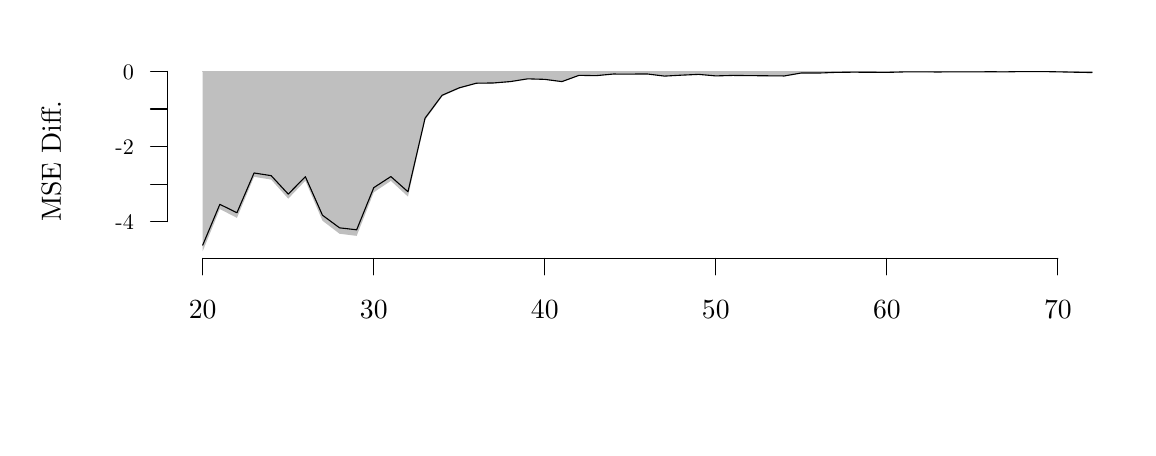
\begin{tikzpicture}[x=1pt,y=1pt]
\definecolor[named]{fillColor}{rgb}{1.00,1.00,1.00}
\path[use as bounding box,fill=fillColor,fill opacity=0.00] (0,0) rectangle (397.48,144.54);
\begin{scope}
\path[clip] ( 50.40, 61.20) rectangle (397.48,131.34);
\definecolor[named]{drawColor}{rgb}{1.00,1.00,1.00}

\path[draw=drawColor,line width= 0.3pt,line join=round,line cap=round] ( 63.25, 63.80) --
	( 69.44, 79.00) --
	( 75.62, 75.81) --
	( 81.80, 90.65) --
	( 87.98, 89.65) --
	( 94.16, 82.75) --
	(100.34, 89.24) --
	(106.52, 74.79) --
	(112.70, 70.07) --
	(118.88, 69.31) --
	(125.06, 85.04) --
	(131.24, 89.19) --
	(137.42, 83.50) --
	(143.60,111.13) --
	(149.78,119.75) --
	(155.96,122.55) --
	(162.14,124.28) --
	(168.32,124.38) --
	(174.50,124.90) --
	(180.68,125.93) --
	(186.86,125.73) --
	(193.04,124.88) --
	(199.22,127.25) --
	(205.40,127.14) --
	(211.58,127.74) --
	(217.76,127.73) --
	(223.94,127.76) --
	(230.12,126.96) --
	(236.30,127.32) --
	(242.48,127.60) --
	(248.66,127.03) --
	(254.84,127.21) --
	(261.02,127.14) --
	(267.20,127.07) --
	(273.38,127.01) --
	(279.57,128.12) --
	(285.75,128.10) --
	(291.93,128.34) --
	(298.11,128.42) --
	(304.29,128.39) --
	(310.47,128.33) --
	(316.65,128.52) --
	(322.83,128.54) --
	(329.01,128.49) --
	(335.19,128.54) --
	(341.37,128.53) --
	(347.55,128.56) --
	(353.73,128.53) --
	(359.91,128.64) --
	(366.09,128.64) --
	(372.27,128.53) --
	(378.45,128.38) --
	(384.63,128.25);

\path[draw=drawColor,line width= 0.3pt,line join=round,line cap=round] ( 63.25, 65.95) --
	( 69.44, 80.70) --
	( 75.62, 77.67) --
	( 81.80, 92.03) --
	( 87.98, 91.07) --
	( 94.16, 84.40) --
	(100.34, 90.69) --
	(106.52, 76.77) --
	(112.70, 72.21) --
	(118.88, 71.50) --
	(125.06, 86.73) --
	(131.24, 90.74) --
	(137.42, 85.25) --
	(143.60,111.86) --
	(149.78,120.13) --
	(155.96,122.81) --
	(162.14,124.47) --
	(168.32,124.56) --
	(174.50,125.07) --
	(180.68,126.05) --
	(186.86,125.86) --
	(193.04,125.05) --
	(199.22,127.31) --
	(205.40,127.20) --
	(211.58,127.78) --
	(217.76,127.77) --
	(223.94,127.80) --
	(230.12,127.04) --
	(236.30,127.38) --
	(242.48,127.66) --
	(248.66,127.11) --
	(254.84,127.28) --
	(261.02,127.21) --
	(267.20,127.15) --
	(273.38,127.09) --
	(279.57,128.17) --
	(285.75,128.14) --
	(291.93,128.38) --
	(298.11,128.46) --
	(304.29,128.43) --
	(310.47,128.38) --
	(316.65,128.55) --
	(322.83,128.57) --
	(329.01,128.53) --
	(335.19,128.58) --
	(341.37,128.57) --
	(347.55,128.60) --
	(353.73,128.58) --
	(359.91,128.68) --
	(366.09,128.68) --
	(372.27,128.58) --
	(378.45,128.44) --
	(384.63,128.32);

\path[draw=drawColor,line width= 0.3pt,line join=round,line cap=round] ( 63.25,128.74) --
	( 69.44,128.74) --
	( 75.62,128.74) --
	( 81.80,128.74) --
	( 87.98,128.74) --
	( 94.16,128.74) --
	(100.34,128.74) --
	(106.52,128.74) --
	(112.70,128.74) --
	(118.88,128.74) --
	(125.06,128.74) --
	(131.24,128.74) --
	(137.42,128.74) --
	(143.60,128.74) --
	(149.78,128.74) --
	(155.96,128.74) --
	(162.14,128.74) --
	(168.32,128.74) --
	(174.50,128.74) --
	(180.68,128.74) --
	(186.86,128.74) --
	(193.04,128.74) --
	(199.22,128.74) --
	(205.40,128.74) --
	(211.58,128.74) --
	(217.76,128.74) --
	(223.94,128.74) --
	(230.12,128.74) --
	(236.30,128.74) --
	(242.48,128.74) --
	(248.66,128.74) --
	(254.84,128.74) --
	(261.02,128.74) --
	(267.20,128.74) --
	(273.38,128.74) --
	(279.57,128.74) --
	(285.75,128.74) --
	(291.93,128.74) --
	(298.11,128.74) --
	(304.29,128.74) --
	(310.47,128.74) --
	(316.65,128.74) --
	(322.83,128.74) --
	(329.01,128.74) --
	(335.19,128.74) --
	(341.37,128.74) --
	(347.55,128.74) --
	(353.73,128.74) --
	(359.91,128.74) --
	(366.09,128.74) --
	(372.27,128.74) --
	(378.45,128.74) --
	(384.63,128.74);
\end{scope}
\begin{scope}
\path[clip] (  0.00,  0.00) rectangle (397.48,144.54);
\definecolor[named]{drawColor}{rgb}{0.00,0.00,0.00}

\node[text=drawColor,rotate= 90.00,anchor=base,inner sep=0pt, outer sep=0pt, scale=  1.00] at ( 12.00, 96.27) {MSE Diff.};
\end{scope}
\begin{scope}
\path[clip] (  0.00,  0.00) rectangle (397.48,144.54);
\definecolor[named]{drawColor}{rgb}{0.00,0.00,0.00}

\path[draw=drawColor,line width= 0.4pt,line join=round,line cap=round] ( 63.25, 61.20) -- (372.27, 61.20);

\path[draw=drawColor,line width= 0.4pt,line join=round,line cap=round] ( 63.25, 61.20) -- ( 63.25, 55.20);

\path[draw=drawColor,line width= 0.4pt,line join=round,line cap=round] (125.06, 61.20) -- (125.06, 55.20);

\path[draw=drawColor,line width= 0.4pt,line join=round,line cap=round] (186.86, 61.20) -- (186.86, 55.20);

\path[draw=drawColor,line width= 0.4pt,line join=round,line cap=round] (248.66, 61.20) -- (248.66, 55.20);

\path[draw=drawColor,line width= 0.4pt,line join=round,line cap=round] (310.47, 61.20) -- (310.47, 55.20);

\path[draw=drawColor,line width= 0.4pt,line join=round,line cap=round] (372.27, 61.20) -- (372.27, 55.20);

\node[text=drawColor,anchor=base,inner sep=0pt, outer sep=0pt, scale=  1.00] at ( 63.25, 39.60) {20};

\node[text=drawColor,anchor=base,inner sep=0pt, outer sep=0pt, scale=  1.00] at (125.06, 39.60) {30};

\node[text=drawColor,anchor=base,inner sep=0pt, outer sep=0pt, scale=  1.00] at (186.86, 39.60) {40};

\node[text=drawColor,anchor=base,inner sep=0pt, outer sep=0pt, scale=  1.00] at (248.66, 39.60) {50};

\node[text=drawColor,anchor=base,inner sep=0pt, outer sep=0pt, scale=  1.00] at (310.47, 39.60) {60};

\node[text=drawColor,anchor=base,inner sep=0pt, outer sep=0pt, scale=  1.00] at (372.27, 39.60) {70};
\end{scope}
\begin{scope}
\path[clip] ( 50.40, 61.20) rectangle (397.48,131.34);
\definecolor[named]{fillColor}{rgb}{0.75,0.75,0.75}

\path[fill=fillColor] ( 63.25,128.74) --
	( 63.25, 63.80) --
	( 69.44, 79.00) --
	( 75.62, 75.81) --
	( 81.80, 90.65) --
	( 87.98, 89.65) --
	( 94.16, 82.75) --
	(100.34, 89.24) --
	(106.52, 74.79) --
	(112.70, 70.07) --
	(118.88, 69.31) --
	(125.06, 85.04) --
	(131.24, 89.19) --
	(137.42, 83.50) --
	(143.60,111.13) --
	(149.78,119.75) --
	(155.96,122.55) --
	(162.14,124.28) --
	(168.32,124.38) --
	(174.50,124.90) --
	(180.68,125.93) --
	(186.86,125.73) --
	(193.04,124.88) --
	(199.22,127.25) --
	(205.40,127.14) --
	(211.58,127.74) --
	(217.76,127.73) --
	(223.94,127.76) --
	(230.12,126.96) --
	(236.30,127.32) --
	(242.48,127.60) --
	(248.66,127.03) --
	(254.84,127.21) --
	(261.02,127.14) --
	(267.20,127.07) --
	(273.38,127.01) --
	(279.57,128.12) --
	(285.75,128.10) --
	(291.93,128.34) --
	(298.11,128.42) --
	(304.29,128.39) --
	(310.47,128.33) --
	(316.65,128.52) --
	(322.83,128.54) --
	(329.01,128.49) --
	(335.19,128.54) --
	(341.37,128.53) --
	(347.55,128.56) --
	(353.73,128.53) --
	(359.91,128.64) --
	(366.09,128.64) --
	(372.27,128.53) --
	(378.45,128.38) --
	(384.63,128.25) --
	(384.63,128.74) --
	cycle;
\definecolor[named]{drawColor}{rgb}{0.75,0.75,0.75}

\path[draw=drawColor,line width= 0.4pt,line join=round,line cap=round] ( 63.25,128.74) --
	(384.63,128.74);
\definecolor[named]{drawColor}{rgb}{0.00,0.00,0.00}

\path[draw=drawColor,line width= 0.4pt,line join=round,line cap=round] ( 63.25, 65.95) --
	( 69.44, 80.70) --
	( 75.62, 77.67) --
	( 81.80, 92.03) --
	( 87.98, 91.07) --
	( 94.16, 84.40) --
	(100.34, 90.69) --
	(106.52, 76.77) --
	(112.70, 72.21) --
	(118.88, 71.50) --
	(125.06, 86.73) --
	(131.24, 90.74) --
	(137.42, 85.25) --
	(143.60,111.86) --
	(149.78,120.13) --
	(155.96,122.81) --
	(162.14,124.47) --
	(168.32,124.56) --
	(174.50,125.07) --
	(180.68,126.05) --
	(186.86,125.86) --
	(193.04,125.05) --
	(199.22,127.31) --
	(205.40,127.20) --
	(211.58,127.78) --
	(217.76,127.77) --
	(223.94,127.80) --
	(230.12,127.04) --
	(236.30,127.38) --
	(242.48,127.66) --
	(248.66,127.11) --
	(254.84,127.28) --
	(261.02,127.21) --
	(267.20,127.15) --
	(273.38,127.09) --
	(279.57,128.17) --
	(285.75,128.14) --
	(291.93,128.38) --
	(298.11,128.46) --
	(304.29,128.43) --
	(310.47,128.38) --
	(316.65,128.55) --
	(322.83,128.57) --
	(329.01,128.53) --
	(335.19,128.58) --
	(341.37,128.57) --
	(347.55,128.60) --
	(353.73,128.58) --
	(359.91,128.68) --
	(366.09,128.68) --
	(372.27,128.58) --
	(378.45,128.44) --
	(384.63,128.32);
\end{scope}
\begin{scope}
\path[clip] (  0.00,  0.00) rectangle (397.48,144.54);
\definecolor[named]{drawColor}{rgb}{0.00,0.00,0.00}

\path[draw=drawColor,line width= 0.4pt,line join=round,line cap=round] ( 50.40, 74.43) -- ( 50.40,128.74);

\path[draw=drawColor,line width= 0.4pt,line join=round,line cap=round] ( 50.40, 74.43) -- ( 44.40, 74.43);

\path[draw=drawColor,line width= 0.4pt,line join=round,line cap=round] ( 50.40, 88.01) -- ( 44.40, 88.01);

\path[draw=drawColor,line width= 0.4pt,line join=round,line cap=round] ( 50.40,101.59) -- ( 44.40,101.59);

\path[draw=drawColor,line width= 0.4pt,line join=round,line cap=round] ( 50.40,115.16) -- ( 44.40,115.16);

\path[draw=drawColor,line width= 0.4pt,line join=round,line cap=round] ( 50.40,128.74) -- ( 44.40,128.74);

\node[text=drawColor,anchor=base east,inner sep=0pt, outer sep=0pt, scale=  0.80] at ( 38.40, 71.68) {-4};

\node[text=drawColor,anchor=base east,inner sep=0pt, outer sep=0pt, scale=  0.80] at ( 38.40, 98.83) {-2};

\node[text=drawColor,anchor=base east,inner sep=0pt, outer sep=0pt, scale=  0.80] at ( 38.40,125.99) {0};
\end{scope}
\end{tikzpicture}

% Created by tikzDevice version 0.6.2-92-0ad2792 on 2014-03-27 04:41:27
% !TEX encoding = UTF-8 Unicode
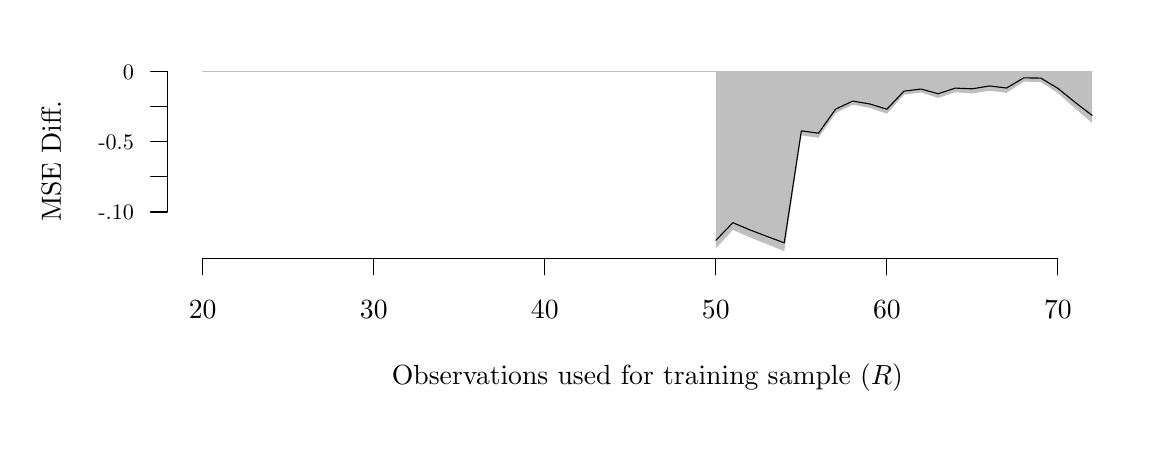
\begin{tikzpicture}[x=1pt,y=1pt]
\definecolor[named]{fillColor}{rgb}{1.00,1.00,1.00}
\path[use as bounding box,fill=fillColor,fill opacity=0.00] (0,0) rectangle (397.48,144.54);
\begin{scope}
\path[clip] ( 50.40, 61.20) rectangle (397.48,131.34);
\definecolor[named]{drawColor}{rgb}{1.00,1.00,1.00}

\path[draw=drawColor,line width= 0.3pt,line join=round,line cap=round] (248.66, 64.79) --
	(254.84, 71.45) --
	(261.02, 68.74) --
	(267.20, 66.28) --
	(273.38, 63.80) --
	(279.57,105.64) --
	(285.75,104.73) --
	(291.93,113.66) --
	(298.11,116.70) --
	(304.29,115.54) --
	(310.47,113.47) --
	(316.65,120.29) --
	(322.83,121.13) --
	(329.01,119.16) --
	(335.19,121.19) --
	(341.37,120.79) --
	(347.55,121.75) --
	(353.73,120.97) --
	(359.91,125.03) --
	(366.09,124.93) --
	(372.27,120.92) --
	(378.45,115.37) --
	(384.63,110.14);

\path[draw=drawColor,line width= 0.3pt,line join=round,line cap=round] (248.66, 67.69) --
	(254.84, 74.06) --
	(261.02, 71.45) --
	(267.20, 69.09) --
	(273.38, 66.79) --
	(279.57,107.26) --
	(285.75,106.40) --
	(291.93,115.08) --
	(298.11,118.01) --
	(304.29,116.97) --
	(310.47,115.08) --
	(316.65,121.60) --
	(322.83,122.36) --
	(329.01,120.66) --
	(335.19,122.70) --
	(341.37,122.44) --
	(347.55,123.48) --
	(353.73,122.73) --
	(359.91,126.40) --
	(366.09,126.32) --
	(372.27,122.61) --
	(378.45,117.59) --
	(384.63,112.83);

\path[draw=drawColor,line width= 0.3pt,line join=round,line cap=round] ( 63.25,128.74) --
	( 69.44,128.74) --
	( 75.62,128.74) --
	( 81.80,128.74) --
	( 87.98,128.74) --
	( 94.16,128.74) --
	(100.34,128.74) --
	(106.52,128.74) --
	(112.70,128.74) --
	(118.88,128.74) --
	(125.06,128.74) --
	(131.24,128.74) --
	(137.42,128.74) --
	(143.60,128.74) --
	(149.78,128.74) --
	(155.96,128.74) --
	(162.14,128.74) --
	(168.32,128.74) --
	(174.50,128.74) --
	(180.68,128.74) --
	(186.86,128.74) --
	(193.04,128.74) --
	(199.22,128.74) --
	(205.40,128.74) --
	(211.58,128.74) --
	(217.76,128.74) --
	(223.94,128.74) --
	(230.12,128.74) --
	(236.30,128.74) --
	(242.48,128.74) --
	(248.66,128.74) --
	(254.84,128.74) --
	(261.02,128.74) --
	(267.20,128.74) --
	(273.38,128.74) --
	(279.57,128.74) --
	(285.75,128.74) --
	(291.93,128.74) --
	(298.11,128.74) --
	(304.29,128.74) --
	(310.47,128.74) --
	(316.65,128.74) --
	(322.83,128.74) --
	(329.01,128.74) --
	(335.19,128.74) --
	(341.37,128.74) --
	(347.55,128.74) --
	(353.73,128.74) --
	(359.91,128.74) --
	(366.09,128.74) --
	(372.27,128.74) --
	(378.45,128.74) --
	(384.63,128.74);
\end{scope}
\begin{scope}
\path[clip] (  0.00,  0.00) rectangle (397.48,144.54);
\definecolor[named]{drawColor}{rgb}{0.00,0.00,0.00}

\node[text=drawColor,anchor=base,inner sep=0pt, outer sep=0pt, scale=  1.00] at (223.94, 15.60) {Observations used for training sample ($R$)};

\node[text=drawColor,rotate= 90.00,anchor=base,inner sep=0pt, outer sep=0pt, scale=  1.00] at ( 12.00, 96.27) {MSE Diff.};
\end{scope}
\begin{scope}
\path[clip] (  0.00,  0.00) rectangle (397.48,144.54);
\definecolor[named]{drawColor}{rgb}{0.00,0.00,0.00}

\path[draw=drawColor,line width= 0.4pt,line join=round,line cap=round] ( 63.25, 61.20) -- (372.27, 61.20);

\path[draw=drawColor,line width= 0.4pt,line join=round,line cap=round] ( 63.25, 61.20) -- ( 63.25, 55.20);

\path[draw=drawColor,line width= 0.4pt,line join=round,line cap=round] (125.06, 61.20) -- (125.06, 55.20);

\path[draw=drawColor,line width= 0.4pt,line join=round,line cap=round] (186.86, 61.20) -- (186.86, 55.20);

\path[draw=drawColor,line width= 0.4pt,line join=round,line cap=round] (248.66, 61.20) -- (248.66, 55.20);

\path[draw=drawColor,line width= 0.4pt,line join=round,line cap=round] (310.47, 61.20) -- (310.47, 55.20);

\path[draw=drawColor,line width= 0.4pt,line join=round,line cap=round] (372.27, 61.20) -- (372.27, 55.20);

\node[text=drawColor,anchor=base,inner sep=0pt, outer sep=0pt, scale=  1.00] at ( 63.25, 39.60) {20};

\node[text=drawColor,anchor=base,inner sep=0pt, outer sep=0pt, scale=  1.00] at (125.06, 39.60) {30};

\node[text=drawColor,anchor=base,inner sep=0pt, outer sep=0pt, scale=  1.00] at (186.86, 39.60) {40};

\node[text=drawColor,anchor=base,inner sep=0pt, outer sep=0pt, scale=  1.00] at (248.66, 39.60) {50};

\node[text=drawColor,anchor=base,inner sep=0pt, outer sep=0pt, scale=  1.00] at (310.47, 39.60) {60};

\node[text=drawColor,anchor=base,inner sep=0pt, outer sep=0pt, scale=  1.00] at (372.27, 39.60) {70};
\end{scope}
\begin{scope}
\path[clip] ( 50.40, 61.20) rectangle (397.48,131.34);
\definecolor[named]{fillColor}{rgb}{0.75,0.75,0.75}

\path[fill=fillColor] (248.66,128.74) --
	(248.66, 64.79) --
	(254.84, 71.45) --
	(261.02, 68.74) --
	(267.20, 66.28) --
	(273.38, 63.80) --
	(279.57,105.64) --
	(285.75,104.73) --
	(291.93,113.66) --
	(298.11,116.70) --
	(304.29,115.54) --
	(310.47,113.47) --
	(316.65,120.29) --
	(322.83,121.13) --
	(329.01,119.16) --
	(335.19,121.19) --
	(341.37,120.79) --
	(347.55,121.75) --
	(353.73,120.97) --
	(359.91,125.03) --
	(366.09,124.93) --
	(372.27,120.92) --
	(378.45,115.37) --
	(384.63,110.14) --
	(384.63,128.74) --
	cycle;
\definecolor[named]{drawColor}{rgb}{0.75,0.75,0.75}

\path[draw=drawColor,line width= 0.4pt,line join=round,line cap=round] ( 63.25,128.74) --
	(384.63,128.74);
\definecolor[named]{drawColor}{rgb}{0.00,0.00,0.00}

\path[draw=drawColor,line width= 0.4pt,line join=round,line cap=round] (248.66, 67.69) --
	(254.84, 74.06) --
	(261.02, 71.45) --
	(267.20, 69.09) --
	(273.38, 66.79) --
	(279.57,107.26) --
	(285.75,106.40) --
	(291.93,115.08) --
	(298.11,118.01) --
	(304.29,116.97) --
	(310.47,115.08) --
	(316.65,121.60) --
	(322.83,122.36) --
	(329.01,120.66) --
	(335.19,122.70) --
	(341.37,122.44) --
	(347.55,123.48) --
	(353.73,122.73) --
	(359.91,126.40) --
	(366.09,126.32) --
	(372.27,122.61) --
	(378.45,117.59) --
	(384.63,112.83);
\end{scope}
\begin{scope}
\path[clip] (  0.00,  0.00) rectangle (397.48,144.54);
\definecolor[named]{drawColor}{rgb}{0.00,0.00,0.00}

\path[draw=drawColor,line width= 0.4pt,line join=round,line cap=round] ( 50.40, 77.95) -- ( 50.40,128.74);

\path[draw=drawColor,line width= 0.4pt,line join=round,line cap=round] ( 50.40, 77.95) -- ( 44.40, 77.95);

\path[draw=drawColor,line width= 0.4pt,line join=round,line cap=round] ( 50.40, 90.65) -- ( 44.40, 90.65);

\path[draw=drawColor,line width= 0.4pt,line join=round,line cap=round] ( 50.40,103.34) -- ( 44.40,103.34);

\path[draw=drawColor,line width= 0.4pt,line join=round,line cap=round] ( 50.40,116.04) -- ( 44.40,116.04);

\path[draw=drawColor,line width= 0.4pt,line join=round,line cap=round] ( 50.40,128.74) -- ( 44.40,128.74);

\node[text=drawColor,anchor=base east,inner sep=0pt, outer sep=0pt, scale=  0.80] at ( 38.40, 75.19) {-.10};

\node[text=drawColor,anchor=base east,inner sep=0pt, outer sep=0pt, scale=  0.80] at ( 38.40,100.59) {-0.5};

\node[text=drawColor,anchor=base east,inner sep=0pt, outer sep=0pt, scale=  0.80] at ( 38.40,125.99) {0};
\end{scope}
\end{tikzpicture}

\caption{OOS difference in the MSE
  of the prevailing mean benchmark and the kitchen sink model as a
  function of the test sample size, $R$.  Both models forecast the
  equity premium using annual data from 1928--2008.  The solid line
  gives the OOS average, and the shaded region indicates the
  one-sided 95\% confidence interval implied by the
  DMW test.  The bottom panel is a detailed view of the top
  panel for $R \geq 50$.}
\label{fig:empirics1}
\end{figure}

\begin{figure}
\centering
\large{Difference in OOS MSE of Prevailing Mean and\\ Kitchen
    Sink Models of Equity Premium (CT)}
% Created by tikzDevice version 0.6.2-92-0ad2792 on 2014-03-27 04:41:27
% !TEX encoding = UTF-8 Unicode
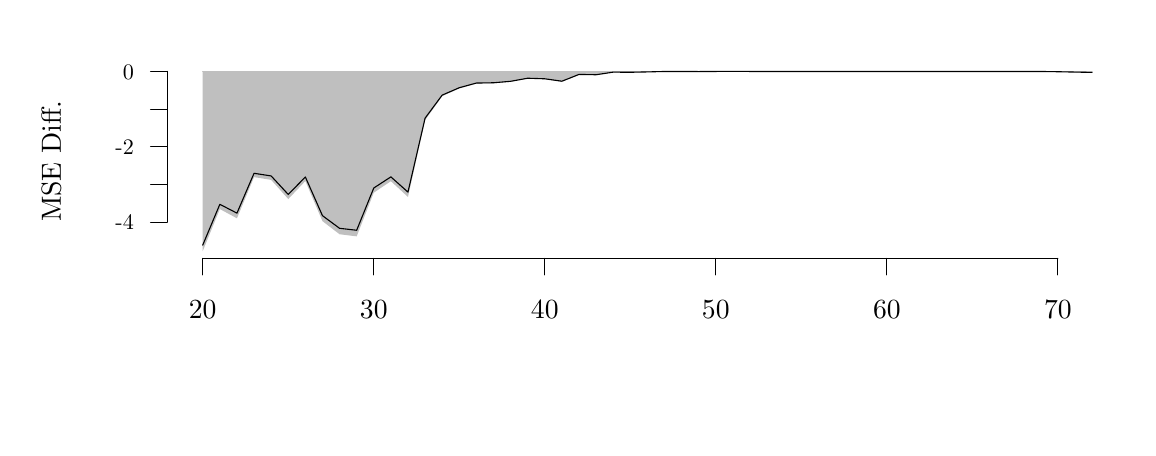
\begin{tikzpicture}[x=1pt,y=1pt]
\definecolor[named]{fillColor}{rgb}{1.00,1.00,1.00}
\path[use as bounding box,fill=fillColor,fill opacity=0.00] (0,0) rectangle (397.48,144.54);
\begin{scope}
\path[clip] ( 50.40, 61.20) rectangle (397.48,131.34);
\definecolor[named]{drawColor}{rgb}{1.00,1.00,1.00}

\path[draw=drawColor,line width= 0.3pt,line join=round,line cap=round] ( 63.25, 63.80) --
	( 69.44, 79.00) --
	( 75.62, 75.65) --
	( 81.80, 90.54) --
	( 87.98, 89.54) --
	( 94.16, 82.61) --
	(100.34, 89.12) --
	(106.52, 74.63) --
	(112.70, 69.89) --
	(118.88, 69.13) --
	(125.06, 84.91) --
	(131.24, 89.07) --
	(137.42, 83.37) --
	(143.60,111.11) --
	(149.78,119.79) --
	(155.96,122.58) --
	(162.14,124.34) --
	(168.32,124.44) --
	(174.50,124.99) --
	(180.68,126.15) --
	(186.86,125.94) --
	(193.04,125.01) --
	(199.22,127.58) --
	(205.40,127.46) --
	(211.58,128.46) --
	(217.76,128.40) --
	(223.94,128.54) --
	(230.12,128.70) --
	(236.30,128.70) --
	(242.48,128.68) --
	(248.66,128.71) --
	(254.84,128.72) --
	(261.02,128.72) --
	(267.20,128.71) --
	(273.38,128.71) --
	(279.57,128.69) --
	(285.75,128.71) --
	(291.93,128.71) --
	(298.11,128.71) --
	(304.29,128.70) --
	(310.47,128.70) --
	(316.65,128.70) --
	(322.83,128.69) --
	(329.01,128.70) --
	(335.19,128.71) --
	(341.37,128.71) --
	(347.55,128.71) --
	(353.73,128.70) --
	(359.91,128.70) --
	(366.09,128.68) --
	(372.27,128.59) --
	(378.45,128.44) --
	(384.63,128.30);

\path[draw=drawColor,line width= 0.3pt,line join=round,line cap=round] ( 63.25, 65.95) --
	( 69.44, 80.71) --
	( 75.62, 77.52) --
	( 81.80, 91.92) --
	( 87.98, 90.96) --
	( 94.16, 84.27) --
	(100.34, 90.58) --
	(106.52, 76.61) --
	(112.70, 72.04) --
	(118.88, 71.33) --
	(125.06, 86.60) --
	(131.24, 90.62) --
	(137.42, 85.12) --
	(143.60,111.84) --
	(149.78,120.17) --
	(155.96,122.84) --
	(162.14,124.53) --
	(168.32,124.63) --
	(174.50,125.16) --
	(180.68,126.27) --
	(186.86,126.07) --
	(193.04,125.19) --
	(199.22,127.64) --
	(205.40,127.53) --
	(211.58,128.47) --
	(217.76,128.42) --
	(223.94,128.55) --
	(230.12,128.71) --
	(236.30,128.71) --
	(242.48,128.68) --
	(248.66,128.72) --
	(254.84,128.73) --
	(261.02,128.72) --
	(267.20,128.72) --
	(273.38,128.71) --
	(279.57,128.70) --
	(285.75,128.72) --
	(291.93,128.72) --
	(298.11,128.72) --
	(304.29,128.72) --
	(310.47,128.71) --
	(316.65,128.72) --
	(322.83,128.70) --
	(329.01,128.71) --
	(335.19,128.72) --
	(341.37,128.72) --
	(347.55,128.72) --
	(353.73,128.72) --
	(359.91,128.72) --
	(366.09,128.71) --
	(372.27,128.62) --
	(378.45,128.49) --
	(384.63,128.37);

\path[draw=drawColor,line width= 0.3pt,line join=round,line cap=round] ( 63.25,128.74) --
	( 69.44,128.74) --
	( 75.62,128.74) --
	( 81.80,128.74) --
	( 87.98,128.74) --
	( 94.16,128.74) --
	(100.34,128.74) --
	(106.52,128.74) --
	(112.70,128.74) --
	(118.88,128.74) --
	(125.06,128.74) --
	(131.24,128.74) --
	(137.42,128.74) --
	(143.60,128.74) --
	(149.78,128.74) --
	(155.96,128.74) --
	(162.14,128.74) --
	(168.32,128.74) --
	(174.50,128.74) --
	(180.68,128.74) --
	(186.86,128.74) --
	(193.04,128.74) --
	(199.22,128.74) --
	(205.40,128.74) --
	(211.58,128.74) --
	(217.76,128.74) --
	(223.94,128.74) --
	(230.12,128.74) --
	(236.30,128.74) --
	(242.48,128.74) --
	(248.66,128.74) --
	(254.84,128.74) --
	(261.02,128.74) --
	(267.20,128.74) --
	(273.38,128.74) --
	(279.57,128.74) --
	(285.75,128.74) --
	(291.93,128.74) --
	(298.11,128.74) --
	(304.29,128.74) --
	(310.47,128.74) --
	(316.65,128.74) --
	(322.83,128.74) --
	(329.01,128.74) --
	(335.19,128.74) --
	(341.37,128.74) --
	(347.55,128.74) --
	(353.73,128.74) --
	(359.91,128.74) --
	(366.09,128.74) --
	(372.27,128.74) --
	(378.45,128.74) --
	(384.63,128.74);
\end{scope}
\begin{scope}
\path[clip] (  0.00,  0.00) rectangle (397.48,144.54);
\definecolor[named]{drawColor}{rgb}{0.00,0.00,0.00}

\node[text=drawColor,rotate= 90.00,anchor=base,inner sep=0pt, outer sep=0pt, scale=  1.00] at ( 12.00, 96.27) {MSE Diff.};
\end{scope}
\begin{scope}
\path[clip] (  0.00,  0.00) rectangle (397.48,144.54);
\definecolor[named]{drawColor}{rgb}{0.00,0.00,0.00}

\path[draw=drawColor,line width= 0.4pt,line join=round,line cap=round] ( 63.25, 61.20) -- (372.27, 61.20);

\path[draw=drawColor,line width= 0.4pt,line join=round,line cap=round] ( 63.25, 61.20) -- ( 63.25, 55.20);

\path[draw=drawColor,line width= 0.4pt,line join=round,line cap=round] (125.06, 61.20) -- (125.06, 55.20);

\path[draw=drawColor,line width= 0.4pt,line join=round,line cap=round] (186.86, 61.20) -- (186.86, 55.20);

\path[draw=drawColor,line width= 0.4pt,line join=round,line cap=round] (248.66, 61.20) -- (248.66, 55.20);

\path[draw=drawColor,line width= 0.4pt,line join=round,line cap=round] (310.47, 61.20) -- (310.47, 55.20);

\path[draw=drawColor,line width= 0.4pt,line join=round,line cap=round] (372.27, 61.20) -- (372.27, 55.20);

\node[text=drawColor,anchor=base,inner sep=0pt, outer sep=0pt, scale=  1.00] at ( 63.25, 39.60) {20};

\node[text=drawColor,anchor=base,inner sep=0pt, outer sep=0pt, scale=  1.00] at (125.06, 39.60) {30};

\node[text=drawColor,anchor=base,inner sep=0pt, outer sep=0pt, scale=  1.00] at (186.86, 39.60) {40};

\node[text=drawColor,anchor=base,inner sep=0pt, outer sep=0pt, scale=  1.00] at (248.66, 39.60) {50};

\node[text=drawColor,anchor=base,inner sep=0pt, outer sep=0pt, scale=  1.00] at (310.47, 39.60) {60};

\node[text=drawColor,anchor=base,inner sep=0pt, outer sep=0pt, scale=  1.00] at (372.27, 39.60) {70};
\end{scope}
\begin{scope}
\path[clip] ( 50.40, 61.20) rectangle (397.48,131.34);
\definecolor[named]{fillColor}{rgb}{0.75,0.75,0.75}

\path[fill=fillColor] ( 63.25,128.74) --
	( 63.25, 63.80) --
	( 69.44, 79.00) --
	( 75.62, 75.65) --
	( 81.80, 90.54) --
	( 87.98, 89.54) --
	( 94.16, 82.61) --
	(100.34, 89.12) --
	(106.52, 74.63) --
	(112.70, 69.89) --
	(118.88, 69.13) --
	(125.06, 84.91) --
	(131.24, 89.07) --
	(137.42, 83.37) --
	(143.60,111.11) --
	(149.78,119.79) --
	(155.96,122.58) --
	(162.14,124.34) --
	(168.32,124.44) --
	(174.50,124.99) --
	(180.68,126.15) --
	(186.86,125.94) --
	(193.04,125.01) --
	(199.22,127.58) --
	(205.40,127.46) --
	(211.58,128.46) --
	(217.76,128.40) --
	(223.94,128.54) --
	(230.12,128.70) --
	(236.30,128.70) --
	(242.48,128.68) --
	(248.66,128.71) --
	(254.84,128.72) --
	(261.02,128.72) --
	(267.20,128.71) --
	(273.38,128.71) --
	(279.57,128.69) --
	(285.75,128.71) --
	(291.93,128.71) --
	(298.11,128.71) --
	(304.29,128.70) --
	(310.47,128.70) --
	(316.65,128.70) --
	(322.83,128.69) --
	(329.01,128.70) --
	(335.19,128.71) --
	(341.37,128.71) --
	(347.55,128.71) --
	(353.73,128.70) --
	(359.91,128.70) --
	(366.09,128.68) --
	(372.27,128.59) --
	(378.45,128.44) --
	(384.63,128.30) --
	(384.63,128.74) --
	cycle;
\definecolor[named]{drawColor}{rgb}{0.75,0.75,0.75}

\path[draw=drawColor,line width= 0.4pt,line join=round,line cap=round] ( 63.25,128.74) --
	(384.63,128.74);
\definecolor[named]{drawColor}{rgb}{0.00,0.00,0.00}

\path[draw=drawColor,line width= 0.4pt,line join=round,line cap=round] ( 63.25, 65.95) --
	( 69.44, 80.71) --
	( 75.62, 77.52) --
	( 81.80, 91.92) --
	( 87.98, 90.96) --
	( 94.16, 84.27) --
	(100.34, 90.58) --
	(106.52, 76.61) --
	(112.70, 72.04) --
	(118.88, 71.33) --
	(125.06, 86.60) --
	(131.24, 90.62) --
	(137.42, 85.12) --
	(143.60,111.84) --
	(149.78,120.17) --
	(155.96,122.84) --
	(162.14,124.53) --
	(168.32,124.63) --
	(174.50,125.16) --
	(180.68,126.27) --
	(186.86,126.07) --
	(193.04,125.19) --
	(199.22,127.64) --
	(205.40,127.53) --
	(211.58,128.47) --
	(217.76,128.42) --
	(223.94,128.55) --
	(230.12,128.71) --
	(236.30,128.71) --
	(242.48,128.68) --
	(248.66,128.72) --
	(254.84,128.73) --
	(261.02,128.72) --
	(267.20,128.72) --
	(273.38,128.71) --
	(279.57,128.70) --
	(285.75,128.72) --
	(291.93,128.72) --
	(298.11,128.72) --
	(304.29,128.72) --
	(310.47,128.71) --
	(316.65,128.72) --
	(322.83,128.70) --
	(329.01,128.71) --
	(335.19,128.72) --
	(341.37,128.72) --
	(347.55,128.72) --
	(353.73,128.72) --
	(359.91,128.72) --
	(366.09,128.71) --
	(372.27,128.62) --
	(378.45,128.49) --
	(384.63,128.37);
\end{scope}
\begin{scope}
\path[clip] (  0.00,  0.00) rectangle (397.48,144.54);
\definecolor[named]{drawColor}{rgb}{0.00,0.00,0.00}

\path[draw=drawColor,line width= 0.4pt,line join=round,line cap=round] ( 50.40, 74.27) -- ( 50.40,128.74);

\path[draw=drawColor,line width= 0.4pt,line join=round,line cap=round] ( 50.40, 74.27) -- ( 44.40, 74.27);

\path[draw=drawColor,line width= 0.4pt,line join=round,line cap=round] ( 50.40, 87.89) -- ( 44.40, 87.89);

\path[draw=drawColor,line width= 0.4pt,line join=round,line cap=round] ( 50.40,101.51) -- ( 44.40,101.51);

\path[draw=drawColor,line width= 0.4pt,line join=round,line cap=round] ( 50.40,115.12) -- ( 44.40,115.12);

\path[draw=drawColor,line width= 0.4pt,line join=round,line cap=round] ( 50.40,128.74) -- ( 44.40,128.74);

\node[text=drawColor,anchor=base east,inner sep=0pt, outer sep=0pt, scale=  0.80] at ( 38.40, 71.51) {-4};

\node[text=drawColor,anchor=base east,inner sep=0pt, outer sep=0pt, scale=  0.80] at ( 38.40, 98.75) {-2};

\node[text=drawColor,anchor=base east,inner sep=0pt, outer sep=0pt, scale=  0.80] at ( 38.40,125.99) {0};
\end{scope}
\end{tikzpicture}

% Created by tikzDevice version 0.6.2-92-0ad2792 on 2014-03-27 04:41:27
% !TEX encoding = UTF-8 Unicode
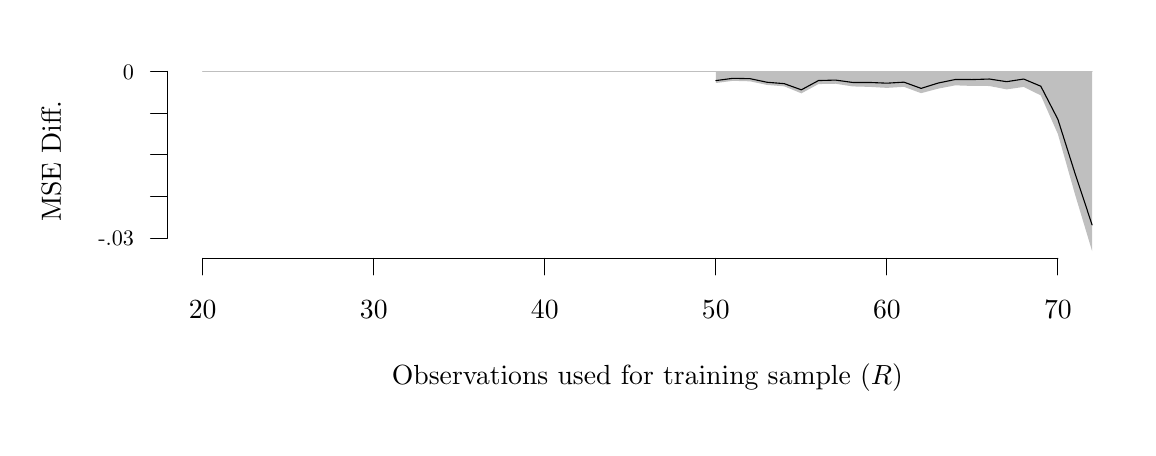
\begin{tikzpicture}[x=1pt,y=1pt]
\definecolor[named]{fillColor}{rgb}{1.00,1.00,1.00}
\path[use as bounding box,fill=fillColor,fill opacity=0.00] (0,0) rectangle (397.48,144.54);
\begin{scope}
\path[clip] ( 50.40, 61.20) rectangle (397.48,131.34);
\definecolor[named]{drawColor}{rgb}{1.00,1.00,1.00}

\path[draw=drawColor,line width= 0.3pt,line join=round,line cap=round] (248.66,124.54) --
	(254.84,125.33) --
	(261.02,125.15) --
	(267.20,123.84) --
	(273.38,123.35) --
	(279.57,120.81) --
	(285.75,124.16) --
	(291.93,124.28) --
	(298.11,123.31) --
	(304.29,123.14) --
	(310.47,122.78) --
	(316.65,123.16) --
	(322.83,120.87) --
	(329.01,122.51) --
	(335.19,123.70) --
	(341.37,123.48) --
	(347.55,123.46) --
	(353.73,122.23) --
	(359.91,123.13) --
	(366.09,120.07) --
	(372.27,106.08) --
	(378.45, 84.32) --
	(384.63, 63.80);

\path[draw=drawColor,line width= 0.3pt,line join=round,line cap=round] (248.66,125.42) --
	(254.84,126.24) --
	(261.02,126.11) --
	(267.20,124.81) --
	(273.38,124.31) --
	(279.57,122.08) --
	(285.75,125.43) --
	(291.93,125.60) --
	(298.11,124.74) --
	(304.29,124.74) --
	(310.47,124.48) --
	(316.65,124.85) --
	(322.83,122.60) --
	(329.01,124.53) --
	(335.19,125.81) --
	(341.37,125.79) --
	(347.55,125.98) --
	(353.73,125.02) --
	(359.91,125.98) --
	(366.09,123.38) --
	(372.27,111.40) --
	(378.45, 91.89) --
	(384.63, 73.27);

\path[draw=drawColor,line width= 0.3pt,line join=round,line cap=round] ( 63.25,128.74) --
	( 69.44,128.74) --
	( 75.62,128.74) --
	( 81.80,128.74) --
	( 87.98,128.74) --
	( 94.16,128.74) --
	(100.34,128.74) --
	(106.52,128.74) --
	(112.70,128.74) --
	(118.88,128.74) --
	(125.06,128.74) --
	(131.24,128.74) --
	(137.42,128.74) --
	(143.60,128.74) --
	(149.78,128.74) --
	(155.96,128.74) --
	(162.14,128.74) --
	(168.32,128.74) --
	(174.50,128.74) --
	(180.68,128.74) --
	(186.86,128.74) --
	(193.04,128.74) --
	(199.22,128.74) --
	(205.40,128.74) --
	(211.58,128.74) --
	(217.76,128.74) --
	(223.94,128.74) --
	(230.12,128.74) --
	(236.30,128.74) --
	(242.48,128.74) --
	(248.66,128.74) --
	(254.84,128.74) --
	(261.02,128.74) --
	(267.20,128.74) --
	(273.38,128.74) --
	(279.57,128.74) --
	(285.75,128.74) --
	(291.93,128.74) --
	(298.11,128.74) --
	(304.29,128.74) --
	(310.47,128.74) --
	(316.65,128.74) --
	(322.83,128.74) --
	(329.01,128.74) --
	(335.19,128.74) --
	(341.37,128.74) --
	(347.55,128.74) --
	(353.73,128.74) --
	(359.91,128.74) --
	(366.09,128.74) --
	(372.27,128.74) --
	(378.45,128.74) --
	(384.63,128.74);
\end{scope}
\begin{scope}
\path[clip] (  0.00,  0.00) rectangle (397.48,144.54);
\definecolor[named]{drawColor}{rgb}{0.00,0.00,0.00}

\node[text=drawColor,anchor=base,inner sep=0pt, outer sep=0pt, scale=  1.00] at (223.94, 15.60) {Observations used for training sample ($R$)};

\node[text=drawColor,rotate= 90.00,anchor=base,inner sep=0pt, outer sep=0pt, scale=  1.00] at ( 12.00, 96.27) {MSE Diff.};
\end{scope}
\begin{scope}
\path[clip] (  0.00,  0.00) rectangle (397.48,144.54);
\definecolor[named]{drawColor}{rgb}{0.00,0.00,0.00}

\path[draw=drawColor,line width= 0.4pt,line join=round,line cap=round] ( 63.25, 61.20) -- (372.27, 61.20);

\path[draw=drawColor,line width= 0.4pt,line join=round,line cap=round] ( 63.25, 61.20) -- ( 63.25, 55.20);

\path[draw=drawColor,line width= 0.4pt,line join=round,line cap=round] (125.06, 61.20) -- (125.06, 55.20);

\path[draw=drawColor,line width= 0.4pt,line join=round,line cap=round] (186.86, 61.20) -- (186.86, 55.20);

\path[draw=drawColor,line width= 0.4pt,line join=round,line cap=round] (248.66, 61.20) -- (248.66, 55.20);

\path[draw=drawColor,line width= 0.4pt,line join=round,line cap=round] (310.47, 61.20) -- (310.47, 55.20);

\path[draw=drawColor,line width= 0.4pt,line join=round,line cap=round] (372.27, 61.20) -- (372.27, 55.20);

\node[text=drawColor,anchor=base,inner sep=0pt, outer sep=0pt, scale=  1.00] at ( 63.25, 39.60) {20};

\node[text=drawColor,anchor=base,inner sep=0pt, outer sep=0pt, scale=  1.00] at (125.06, 39.60) {30};

\node[text=drawColor,anchor=base,inner sep=0pt, outer sep=0pt, scale=  1.00] at (186.86, 39.60) {40};

\node[text=drawColor,anchor=base,inner sep=0pt, outer sep=0pt, scale=  1.00] at (248.66, 39.60) {50};

\node[text=drawColor,anchor=base,inner sep=0pt, outer sep=0pt, scale=  1.00] at (310.47, 39.60) {60};

\node[text=drawColor,anchor=base,inner sep=0pt, outer sep=0pt, scale=  1.00] at (372.27, 39.60) {70};
\end{scope}
\begin{scope}
\path[clip] ( 50.40, 61.20) rectangle (397.48,131.34);
\definecolor[named]{fillColor}{rgb}{0.75,0.75,0.75}

\path[fill=fillColor] (248.66,128.74) --
	(248.66,124.54) --
	(254.84,125.33) --
	(261.02,125.15) --
	(267.20,123.84) --
	(273.38,123.35) --
	(279.57,120.81) --
	(285.75,124.16) --
	(291.93,124.28) --
	(298.11,123.31) --
	(304.29,123.14) --
	(310.47,122.78) --
	(316.65,123.16) --
	(322.83,120.87) --
	(329.01,122.51) --
	(335.19,123.70) --
	(341.37,123.48) --
	(347.55,123.46) --
	(353.73,122.23) --
	(359.91,123.13) --
	(366.09,120.07) --
	(372.27,106.08) --
	(378.45, 84.32) --
	(384.63, 63.80) --
	(384.63,128.74) --
	cycle;
\definecolor[named]{drawColor}{rgb}{0.75,0.75,0.75}

\path[draw=drawColor,line width= 0.4pt,line join=round,line cap=round] ( 63.25,128.74) --
	(384.63,128.74);
\definecolor[named]{drawColor}{rgb}{0.00,0.00,0.00}

\path[draw=drawColor,line width= 0.4pt,line join=round,line cap=round] (248.66,125.42) --
	(254.84,126.24) --
	(261.02,126.11) --
	(267.20,124.81) --
	(273.38,124.31) --
	(279.57,122.08) --
	(285.75,125.43) --
	(291.93,125.60) --
	(298.11,124.74) --
	(304.29,124.74) --
	(310.47,124.48) --
	(316.65,124.85) --
	(322.83,122.60) --
	(329.01,124.53) --
	(335.19,125.81) --
	(341.37,125.79) --
	(347.55,125.98) --
	(353.73,125.02) --
	(359.91,125.98) --
	(366.09,123.38) --
	(372.27,111.40) --
	(378.45, 91.89) --
	(384.63, 73.27);
\end{scope}
\begin{scope}
\path[clip] (  0.00,  0.00) rectangle (397.48,144.54);
\definecolor[named]{drawColor}{rgb}{0.00,0.00,0.00}

\path[draw=drawColor,line width= 0.4pt,line join=round,line cap=round] ( 50.40, 68.44) -- ( 50.40,128.74);

\path[draw=drawColor,line width= 0.4pt,line join=round,line cap=round] ( 50.40, 68.44) -- ( 44.40, 68.44);

\path[draw=drawColor,line width= 0.4pt,line join=round,line cap=round] ( 50.40, 83.51) -- ( 44.40, 83.51);

\path[draw=drawColor,line width= 0.4pt,line join=round,line cap=round] ( 50.40, 98.59) -- ( 44.40, 98.59);

\path[draw=drawColor,line width= 0.4pt,line join=round,line cap=round] ( 50.40,113.67) -- ( 44.40,113.67);

\path[draw=drawColor,line width= 0.4pt,line join=round,line cap=round] ( 50.40,128.74) -- ( 44.40,128.74);

\node[text=drawColor,anchor=base east,inner sep=0pt, outer sep=0pt, scale=  0.80] at ( 38.40, 65.68) {-.03};

\node[text=drawColor,anchor=base east,inner sep=0pt, outer sep=0pt, scale=  0.80] at ( 38.40,125.99) {0};
\end{scope}
\end{tikzpicture}

\caption{OOS difference in the MSE
  of the prevailing mean benchmark and the kitchen sink model as a
  function of the test sample size, $R$.  Both models forecast the
  equity premium using annual data from 1928--2008.  The solid line
  gives the OOS average, and the shaded region indicates the
  one-sided 95\% confidence interval implied by the 
  DMW test.  The bottom panel is a detailed view of the top
  panel for $R \geq 50$.}
\label{fig:empirics2}
\end{figure}

\begin{figure}
\centering
\large{OOS MSE of Individual Forecasts of Equity Premium}
% Created by tikzDevice version 0.6.2-92-0ad2792 on 2014-03-27 04:41:27
% !TEX encoding = UTF-8 Unicode
\begin{tikzpicture}[x=1pt,y=1pt]
\definecolor[named]{fillColor}{rgb}{1.00,1.00,1.00}
\path[use as bounding box,fill=fillColor,fill opacity=0.00] (0,0) rectangle (397.48,144.54);
\begin{scope}
\path[clip] ( 50.40, 61.20) rectangle (397.48,131.34);
\definecolor[named]{drawColor}{rgb}{1.00,1.00,1.00}

\path[draw=drawColor,line width= 0.3pt,line join=round,line cap=round] ( 63.25,128.74) --
	( 69.44,113.58) --
	( 75.62,116.70) --
	( 81.80,101.94) --
	( 87.98,102.92) --
	( 94.16,109.79) --
	(100.34,103.33) --
	(106.52,117.62) --
	(112.70,122.31) --
	(118.88,123.05) --
	(125.06,107.38) --
	(131.24,103.26) --
	(137.42,108.90) --
	(143.60, 81.56) --
	(149.78, 73.07) --
	(155.96, 70.30) --
	(162.14, 68.61) --
	(168.32, 68.52) --
	(174.50, 68.01) --
	(180.68, 66.99) --
	(186.86, 67.19) --
	(193.04, 68.04) --
	(199.22, 65.70) --
	(205.40, 65.82) --
	(211.58, 65.23) --
	(217.76, 65.25) --
	(223.94, 65.20) --
	(230.12, 65.91) --
	(236.30, 65.56) --
	(242.48, 65.28) --
	(248.66, 65.84) --
	(254.84, 65.68) --
	(261.02, 65.76) --
	(267.20, 65.83) --
	(273.38, 65.88) --
	(279.57, 64.78) --
	(285.75, 64.82) --
	(291.93, 64.59) --
	(298.11, 64.52) --
	(304.29, 64.56) --
	(310.47, 64.63) --
	(316.65, 64.48) --
	(322.83, 64.47) --
	(329.01, 64.52) --
	(335.19, 64.47) --
	(341.37, 64.51) --
	(347.55, 64.52) --
	(353.73, 64.57) --
	(359.91, 64.47) --
	(366.09, 64.51) --
	(372.27, 64.63) --
	(378.45, 64.81) --
	(384.63, 65.01);

\path[draw=drawColor,line width= 0.3pt,line join=round,line cap=round] ( 63.25, 63.80) --
	( 69.44, 63.80) --
	( 75.62, 63.80) --
	( 81.80, 63.80) --
	( 87.98, 63.80) --
	( 94.16, 63.80) --
	(100.34, 63.80) --
	(106.52, 63.80) --
	(112.70, 63.80) --
	(118.88, 63.80) --
	(125.06, 63.80) --
	(131.24, 63.80) --
	(137.42, 63.80) --
	(143.60, 63.80) --
	(149.78, 63.80) --
	(155.96, 63.80) --
	(162.14, 63.80) --
	(168.32, 63.80) --
	(174.50, 63.80) --
	(180.68, 63.80) --
	(186.86, 63.80) --
	(193.04, 63.80) --
	(199.22, 63.80) --
	(205.40, 63.80) --
	(211.58, 63.80) --
	(217.76, 63.80) --
	(223.94, 63.80) --
	(230.12, 63.80) --
	(236.30, 63.80) --
	(242.48, 63.80) --
	(248.66, 63.80) --
	(254.84, 63.80) --
	(261.02, 63.80) --
	(267.20, 63.80) --
	(273.38, 63.80) --
	(279.57, 63.80) --
	(285.75, 63.80) --
	(291.93, 63.80) --
	(298.11, 63.80) --
	(304.29, 63.80) --
	(310.47, 63.80) --
	(316.65, 63.80) --
	(322.83, 63.80) --
	(329.01, 63.80) --
	(335.19, 63.80) --
	(341.37, 63.80) --
	(347.55, 63.80) --
	(353.73, 63.80) --
	(359.91, 63.80) --
	(366.09, 63.80) --
	(372.27, 63.80) --
	(378.45, 63.80) --
	(384.63, 63.80);
\end{scope}
\begin{scope}
\path[clip] (  0.00,  0.00) rectangle (397.48,144.54);
\definecolor[named]{drawColor}{rgb}{0.00,0.00,0.00}

\node[text=drawColor,rotate= 90.00,anchor=base,inner sep=0pt, outer sep=0pt, scale=  1.00] at ( 12.00, 96.27) {Full model};
\end{scope}
\begin{scope}
\path[clip] (  0.00,  0.00) rectangle (397.48,144.54);
\definecolor[named]{drawColor}{rgb}{0.00,0.00,0.00}

\path[draw=drawColor,line width= 0.4pt,line join=round,line cap=round] ( 63.25, 61.20) -- (372.27, 61.20);

\path[draw=drawColor,line width= 0.4pt,line join=round,line cap=round] ( 63.25, 61.20) -- ( 63.25, 55.20);

\path[draw=drawColor,line width= 0.4pt,line join=round,line cap=round] (125.06, 61.20) -- (125.06, 55.20);

\path[draw=drawColor,line width= 0.4pt,line join=round,line cap=round] (186.86, 61.20) -- (186.86, 55.20);

\path[draw=drawColor,line width= 0.4pt,line join=round,line cap=round] (248.66, 61.20) -- (248.66, 55.20);

\path[draw=drawColor,line width= 0.4pt,line join=round,line cap=round] (310.47, 61.20) -- (310.47, 55.20);

\path[draw=drawColor,line width= 0.4pt,line join=round,line cap=round] (372.27, 61.20) -- (372.27, 55.20);

\node[text=drawColor,anchor=base,inner sep=0pt, outer sep=0pt, scale=  1.00] at ( 63.25, 39.60) {20};

\node[text=drawColor,anchor=base,inner sep=0pt, outer sep=0pt, scale=  1.00] at (125.06, 39.60) {30};

\node[text=drawColor,anchor=base,inner sep=0pt, outer sep=0pt, scale=  1.00] at (186.86, 39.60) {40};

\node[text=drawColor,anchor=base,inner sep=0pt, outer sep=0pt, scale=  1.00] at (248.66, 39.60) {50};

\node[text=drawColor,anchor=base,inner sep=0pt, outer sep=0pt, scale=  1.00] at (310.47, 39.60) {60};

\node[text=drawColor,anchor=base,inner sep=0pt, outer sep=0pt, scale=  1.00] at (372.27, 39.60) {70};
\end{scope}
\begin{scope}
\path[clip] ( 50.40, 61.20) rectangle (397.48,131.34);
\definecolor[named]{drawColor}{rgb}{0.00,0.00,0.00}

\path[draw=drawColor,line width= 0.4pt,line join=round,line cap=round] ( 63.25,128.74) --
	( 69.44,113.58) --
	( 75.62,116.70) --
	( 81.80,101.94) --
	( 87.98,102.92) --
	( 94.16,109.79) --
	(100.34,103.33) --
	(106.52,117.62) --
	(112.70,122.31) --
	(118.88,123.05) --
	(125.06,107.38) --
	(131.24,103.26) --
	(137.42,108.90) --
	(143.60, 81.56) --
	(149.78, 73.07) --
	(155.96, 70.30) --
	(162.14, 68.61) --
	(168.32, 68.52) --
	(174.50, 68.01) --
	(180.68, 66.99) --
	(186.86, 67.19) --
	(193.04, 68.04) --
	(199.22, 65.70) --
	(205.40, 65.82) --
	(211.58, 65.23) --
	(217.76, 65.25) --
	(223.94, 65.20) --
	(230.12, 65.91) --
	(236.30, 65.56) --
	(242.48, 65.28) --
	(248.66, 65.84) --
	(254.84, 65.68) --
	(261.02, 65.76) --
	(267.20, 65.83) --
	(273.38, 65.88) --
	(279.57, 64.78) --
	(285.75, 64.82) --
	(291.93, 64.59) --
	(298.11, 64.52) --
	(304.29, 64.56) --
	(310.47, 64.63) --
	(316.65, 64.48) --
	(322.83, 64.47) --
	(329.01, 64.52) --
	(335.19, 64.47) --
	(341.37, 64.51) --
	(347.55, 64.52) --
	(353.73, 64.57) --
	(359.91, 64.47) --
	(366.09, 64.51) --
	(372.27, 64.63) --
	(378.45, 64.81) --
	(384.63, 65.01);
\end{scope}
\begin{scope}
\path[clip] (  0.00,  0.00) rectangle (397.48,144.54);
\definecolor[named]{drawColor}{rgb}{0.00,0.00,0.00}

\path[draw=drawColor,line width= 0.4pt,line join=round,line cap=round] ( 50.40, 63.80) -- ( 50.40,119.62);

\path[draw=drawColor,line width= 0.4pt,line join=round,line cap=round] ( 50.40, 63.80) -- ( 44.40, 63.80);

\path[draw=drawColor,line width= 0.4pt,line join=round,line cap=round] ( 50.40, 77.75) -- ( 44.40, 77.75);

\path[draw=drawColor,line width= 0.4pt,line join=round,line cap=round] ( 50.40, 91.71) -- ( 44.40, 91.71);

\path[draw=drawColor,line width= 0.4pt,line join=round,line cap=round] ( 50.40,105.66) -- ( 44.40,105.66);

\path[draw=drawColor,line width= 0.4pt,line join=round,line cap=round] ( 50.40,119.62) -- ( 44.40,119.62);

\node[text=drawColor,anchor=base east,inner sep=0pt, outer sep=0pt, scale=  0.80] at ( 38.40, 61.04) {0};

\node[text=drawColor,anchor=base east,inner sep=0pt, outer sep=0pt, scale=  0.80] at ( 38.40, 75.00) {1};

\node[text=drawColor,anchor=base east,inner sep=0pt, outer sep=0pt, scale=  0.80] at ( 38.40, 88.95) {2};

\node[text=drawColor,anchor=base east,inner sep=0pt, outer sep=0pt, scale=  0.80] at ( 38.40,102.91) {3};

\node[text=drawColor,anchor=base east,inner sep=0pt, outer sep=0pt, scale=  0.80] at ( 38.40,116.86) {4};
\end{scope}
\end{tikzpicture}

% Created by tikzDevice version 0.6.2-92-0ad2792 on 2014-03-27 04:41:27
% !TEX encoding = UTF-8 Unicode
\begin{tikzpicture}[x=1pt,y=1pt]
\definecolor[named]{fillColor}{rgb}{1.00,1.00,1.00}
\path[use as bounding box,fill=fillColor,fill opacity=0.00] (0,0) rectangle (397.48,144.54);
\begin{scope}
\path[clip] ( 50.40, 61.20) rectangle (397.48,131.34);
\definecolor[named]{drawColor}{rgb}{1.00,1.00,1.00}

\path[draw=drawColor,line width= 0.3pt,line join=round,line cap=round] ( 63.25, 97.34) --
	( 69.44, 97.88) --
	( 75.62, 98.01) --
	( 81.80, 97.62) --
	( 87.98, 97.87) --
	( 94.16, 98.41) --
	(100.34, 98.76) --
	(106.52, 97.50) --
	(112.70, 97.95) --
	(118.88, 98.43) --
	(125.06, 97.50) --
	(131.24, 97.26) --
	(137.42, 97.93) --
	(143.60, 98.08) --
	(149.78, 98.74) --
	(155.96, 97.99) --
	(162.14, 98.74) --
	(168.32, 99.59) --
	(174.50,100.40) --
	(180.68, 99.28) --
	(186.86,100.08) --
	(193.04,100.89) --
	(199.22, 99.90) --
	(205.40,100.40) --
	(211.58,101.38) --
	(217.76,102.37) --
	(223.94,100.30) --
	(230.12, 94.81) --
	(236.30, 94.33) --
	(242.48, 94.91) --
	(248.66, 94.58) --
	(254.84, 95.42) --
	(261.02, 96.47) --
	(267.20, 97.16) --
	(273.38, 95.89) --
	(279.57, 97.03) --
	(285.75, 98.12) --
	(291.93, 99.14) --
	(298.11, 99.59) --
	(304.29,101.00) --
	(310.47,102.50) --
	(316.65,104.29) --
	(322.83,105.29) --
	(329.01,105.81) --
	(335.19,106.66) --
	(341.37,109.14) --
	(347.55,111.98) --
	(353.73,114.58) --
	(359.91,114.85) --
	(366.09,118.06) --
	(372.27,119.90) --
	(378.45,123.28) --
	(384.63,128.74);

\path[draw=drawColor,line width= 0.3pt,line join=round,line cap=round] ( 63.25, 63.80) --
	( 69.44, 63.80) --
	( 75.62, 63.80) --
	( 81.80, 63.80) --
	( 87.98, 63.80) --
	( 94.16, 63.80) --
	(100.34, 63.80) --
	(106.52, 63.80) --
	(112.70, 63.80) --
	(118.88, 63.80) --
	(125.06, 63.80) --
	(131.24, 63.80) --
	(137.42, 63.80) --
	(143.60, 63.80) --
	(149.78, 63.80) --
	(155.96, 63.80) --
	(162.14, 63.80) --
	(168.32, 63.80) --
	(174.50, 63.80) --
	(180.68, 63.80) --
	(186.86, 63.80) --
	(193.04, 63.80) --
	(199.22, 63.80) --
	(205.40, 63.80) --
	(211.58, 63.80) --
	(217.76, 63.80) --
	(223.94, 63.80) --
	(230.12, 63.80) --
	(236.30, 63.80) --
	(242.48, 63.80) --
	(248.66, 63.80) --
	(254.84, 63.80) --
	(261.02, 63.80) --
	(267.20, 63.80) --
	(273.38, 63.80) --
	(279.57, 63.80) --
	(285.75, 63.80) --
	(291.93, 63.80) --
	(298.11, 63.80) --
	(304.29, 63.80) --
	(310.47, 63.80) --
	(316.65, 63.80) --
	(322.83, 63.80) --
	(329.01, 63.80) --
	(335.19, 63.80) --
	(341.37, 63.80) --
	(347.55, 63.80) --
	(353.73, 63.80) --
	(359.91, 63.80) --
	(366.09, 63.80) --
	(372.27, 63.80) --
	(378.45, 63.80) --
	(384.63, 63.80);
\end{scope}
\begin{scope}
\path[clip] (  0.00,  0.00) rectangle (397.48,144.54);
\definecolor[named]{drawColor}{rgb}{0.00,0.00,0.00}

\node[text=drawColor,anchor=base,inner sep=0pt, outer sep=0pt, scale=  1.00] at (223.94, 15.60) {Observations used for training sample ($R$)};

\node[text=drawColor,rotate= 90.00,anchor=base,inner sep=0pt, outer sep=0pt, scale=  1.00] at ( 12.00, 96.27) {Benchmark};
\end{scope}
\begin{scope}
\path[clip] (  0.00,  0.00) rectangle (397.48,144.54);
\definecolor[named]{drawColor}{rgb}{0.00,0.00,0.00}

\path[draw=drawColor,line width= 0.4pt,line join=round,line cap=round] ( 63.25, 61.20) -- (372.27, 61.20);

\path[draw=drawColor,line width= 0.4pt,line join=round,line cap=round] ( 63.25, 61.20) -- ( 63.25, 55.20);

\path[draw=drawColor,line width= 0.4pt,line join=round,line cap=round] (125.06, 61.20) -- (125.06, 55.20);

\path[draw=drawColor,line width= 0.4pt,line join=round,line cap=round] (186.86, 61.20) -- (186.86, 55.20);

\path[draw=drawColor,line width= 0.4pt,line join=round,line cap=round] (248.66, 61.20) -- (248.66, 55.20);

\path[draw=drawColor,line width= 0.4pt,line join=round,line cap=round] (310.47, 61.20) -- (310.47, 55.20);

\path[draw=drawColor,line width= 0.4pt,line join=round,line cap=round] (372.27, 61.20) -- (372.27, 55.20);

\node[text=drawColor,anchor=base,inner sep=0pt, outer sep=0pt, scale=  1.00] at ( 63.25, 39.60) {20};

\node[text=drawColor,anchor=base,inner sep=0pt, outer sep=0pt, scale=  1.00] at (125.06, 39.60) {30};

\node[text=drawColor,anchor=base,inner sep=0pt, outer sep=0pt, scale=  1.00] at (186.86, 39.60) {40};

\node[text=drawColor,anchor=base,inner sep=0pt, outer sep=0pt, scale=  1.00] at (248.66, 39.60) {50};

\node[text=drawColor,anchor=base,inner sep=0pt, outer sep=0pt, scale=  1.00] at (310.47, 39.60) {60};

\node[text=drawColor,anchor=base,inner sep=0pt, outer sep=0pt, scale=  1.00] at (372.27, 39.60) {70};
\end{scope}
\begin{scope}
\path[clip] ( 50.40, 61.20) rectangle (397.48,131.34);
\definecolor[named]{drawColor}{rgb}{0.00,0.00,0.00}

\path[draw=drawColor,line width= 0.4pt,line join=round,line cap=round] ( 63.25, 97.34) --
	( 69.44, 97.88) --
	( 75.62, 98.01) --
	( 81.80, 97.62) --
	( 87.98, 97.87) --
	( 94.16, 98.41) --
	(100.34, 98.76) --
	(106.52, 97.50) --
	(112.70, 97.95) --
	(118.88, 98.43) --
	(125.06, 97.50) --
	(131.24, 97.26) --
	(137.42, 97.93) --
	(143.60, 98.08) --
	(149.78, 98.74) --
	(155.96, 97.99) --
	(162.14, 98.74) --
	(168.32, 99.59) --
	(174.50,100.40) --
	(180.68, 99.28) --
	(186.86,100.08) --
	(193.04,100.89) --
	(199.22, 99.90) --
	(205.40,100.40) --
	(211.58,101.38) --
	(217.76,102.37) --
	(223.94,100.30) --
	(230.12, 94.81) --
	(236.30, 94.33) --
	(242.48, 94.91) --
	(248.66, 94.58) --
	(254.84, 95.42) --
	(261.02, 96.47) --
	(267.20, 97.16) --
	(273.38, 95.89) --
	(279.57, 97.03) --
	(285.75, 98.12) --
	(291.93, 99.14) --
	(298.11, 99.59) --
	(304.29,101.00) --
	(310.47,102.50) --
	(316.65,104.29) --
	(322.83,105.29) --
	(329.01,105.81) --
	(335.19,106.66) --
	(341.37,109.14) --
	(347.55,111.98) --
	(353.73,114.58) --
	(359.91,114.85) --
	(366.09,118.06) --
	(372.27,119.90) --
	(378.45,123.28) --
	(384.63,128.74);
\end{scope}
\begin{scope}
\path[clip] (  0.00,  0.00) rectangle (397.48,144.54);
\definecolor[named]{drawColor}{rgb}{0.00,0.00,0.00}

\path[draw=drawColor,line width= 0.4pt,line join=round,line cap=round] ( 50.40, 63.80) -- ( 50.40,122.39);

\path[draw=drawColor,line width= 0.4pt,line join=round,line cap=round] ( 50.40, 63.80) -- ( 44.40, 63.80);

\path[draw=drawColor,line width= 0.4pt,line join=round,line cap=round] ( 50.40, 75.52) -- ( 44.40, 75.52);

\path[draw=drawColor,line width= 0.4pt,line join=round,line cap=round] ( 50.40, 87.23) -- ( 44.40, 87.23);

\path[draw=drawColor,line width= 0.4pt,line join=round,line cap=round] ( 50.40, 98.95) -- ( 44.40, 98.95);

\path[draw=drawColor,line width= 0.4pt,line join=round,line cap=round] ( 50.40,110.67) -- ( 44.40,110.67);

\path[draw=drawColor,line width= 0.4pt,line join=round,line cap=round] ( 50.40,122.39) -- ( 44.40,122.39);

\node[text=drawColor,anchor=base east,inner sep=0pt, outer sep=0pt, scale=  0.80] at ( 38.40, 61.04) {0};

\node[text=drawColor,anchor=base east,inner sep=0pt, outer sep=0pt, scale=  0.80] at ( 38.40,119.63) {0.05};
\end{scope}
\end{tikzpicture}

\caption{OOS MSE of the Prevailing Mean (PM) and
    Kitchen Sink (KS) models for equity premium prediction as
    a function of the size of the training sample, $R$.  Please note
    that the vertical scales are different in the two plots.}
\label{fig:empirics3}
\end{figure}

\end{document}

%%% Local Variables:
%%% mode: latex
%%% TeX-master: "paper"
%%% End:

% LocalWords:  McCracken's kilian anatolyev rossi REStud JAppliedEconometrics
% LocalWords:  goyal welch rfs reputational calhoun Berbee's mixingales Rt tS
% LocalWords:  Heteroskedasticity Autocorrelation Tt iT th berbee iS de dx ixz
% LocalWords:  DMW mcleish Rs eq ftestreject lightgray veclen RSQLite zeileis
% LocalWords:  heteroskedasticity hothorn RNews JStatSoftware harrell campbell
% LocalWords:  thompson bivariate Welch's multicollinearity Newey newey tw vw
% LocalWords:  merlevede cltvar dR Scwarz davidson indices lrrrr waldtest Df jt
% LocalWords:  dmw McCracken MSE OLS mse inoue huber elemstatlearning efron sw
% LocalWords:  anova akritas jong normalpart coefpart Jong's rproject rsqlite
% LocalWords:  unrestrictive datasets Heyde's ib oos Mcc MeR StW InK DiM CCS lm
% LocalWords:  ClM CoS ClW GiW GiR GoW Cla HTF Efr BoB AkA AkP DeD Mcl Dej Rde
% LocalWords:  Sar Zeh Zei Har CaT NeW MeP HaH AllRefs Diebold jel Whi RoW brc
% LocalWords:  overrejection overreject fpe JoD iR PeT Giacomini WN Wishart T'V
% LocalWords:  premultiply const overrejects overrejecting BWB Gia Schwarz HHK
% LocalWords:  Haf Anatolyev's nonstochastic T'X Sweave tikzDevice pgfSweave

